%% Hello emacs, this is -*- latex -*-
\typeout{ ====================================================================}
\typeout{ This is file main.tex, created at 23-Jan-2004 }
\typeout{ Maintained by Andre DOS ANJOS <Andre.dos.Anjos@cern.ch> }
\typeout{ ====================================================================}

\documentclass[a4paper,12pt]{report}

%% -----------------------------------------
%% Lista de Pacotes que você deverá precisar
%% -----------------------------------------
\usepackage[french,english,portuges]{babel} % Para hifenação automática.
\usepackage[T1]{fontenc} % Para a hifenação de palavras acentuadas
\usepackage[utf8]{inputenc} % Para tradução automática de acentos.
\usepackage{indentfirst}
\usepackage{tocbibind} % Para a inclusão de bibliografia e índices na ToC
\renewcommand{\tocbibname}{Referências Bibliográficas}

% André DOS ANJOS <Andre.dos.Anjos@cern.ch>
% $Id: mycolor.tex,v 1.1 2002/04/01 19:44:54 andre Exp $

% Entries that are specific to colors
%% Estes comandos aqui definem novas cores. Para usá-las, você tem que
%% incluir no seu fonte, o pacote 'color'
\usepackage{color}
\definecolor{brightred}{rgb}{1,0,0}
\definecolor{red}{rgb}{0.75,0,0}
\definecolor{darkred}{rgb}{0.5,0,0}

\definecolor{brightgreen}{rgb}{0,0.75,0}
\definecolor{green}{rgb}{0,0.5,0}
\definecolor{darkgreen}{rgb}{0,0,0.25}

\definecolor{brightblue}{rgb}{0,0,1}
\definecolor{blue}{rgb}{0,0,0.75}
\definecolor{darkblue}{rgb}{0,0,0.5}
 % Para descrever cores.
% Dear emacs, this is -*- latex -*-
% Andr� DOS ANJOS <Andre.dos.Anjos@cern.ch>
% $Id: ifpdf.tex,v 1.1 2002/04/01 19:44:54 andre Exp $

% Declares the \ifpdf command

\newif\ifpdf
\ifx\pdfoutput\undefined
    \pdffalse          % N�o estamos rodando PDFLaTeX
\else
    \pdfoutput=1       % N�s estamos rodando PDFLaTeX
    \pdftrue
\fi

 % Para a próxima seleção.
\ifpdf % Gráficos, thumbnails e hiper-referências
% André DOS ANJOS <Andre.dos.Anjos@cern.ch>
% $Id: pdfheader.tex,v 1.1 2002/04/01 19:44:54 andre Exp $

% Entries that are specific to process the document with PDFLATEX

% Ligações coloridas
%% \usepackage[pdftex,%
%% 	    colorlinks=true,%
%%             urlcolor=blue,% \href{...}{...}
%%             anchorcolor=brightblue,%
%%             filecolor=green,% \href*{...}
%%             linkcolor=red,% \ref{...} and \pageref{...}
%%             menucolor=darkblue,%
%%             citecolor=darkgreen,%
%%             pdftitle={Tese de Doutorado de André Rabello dos Anjos},%
%%             pdfauthor={Andre Rabello dos Anjos <Andre.dos.Anjos@cern.ch>},%
%%             pdfsubject={Tese},%
%%             pdfkeywords={tese doutorado andre rabello anjos},%
%%             pagebackref,%
%%             pdfpagemode=None,%
%%             bookmarksopen=true]{hyperref}

% Ligações em preto e branco para impressão
\usepackage[pdftex,%
    	    colorlinks=true,%
            urlcolor=black,% \href{...}{...}
            anchorcolor=black,%
            filecolor=black,% \href*{...}
            linkcolor=black,% \ref{...} and \pageref{...}
            menucolor=black,%
            citecolor=black,%
            pdftitle={Tese de Doutorado de Andre Rabello dos Anjos},%
            pdfauthor={Andre DOS ANJOS <Andre.dos.Anjos@cern.ch>},%
            pdfsubject={Tese},%
            pdfkeywords={tese doutorado andre rabello anjos},%
            pagebackref=false,% this enables the back reference at bibitems
            pdfpagemode=None,%
            bookmarksopen=true]{hyperref}
\pdfcompresslevel=9
\usepackage[pdftex]{graphicx}
\DeclareGraphicsExtensions{.pdf,.png,.jpg,.mps}	% modify the preferences
%%\usepackage{thumbpdf}
%%\usepackage{palatino} % try to get closer to adobe tools output


\else
% André DOS ANJOS <Andre.dos.Anjos@cern.ch>
% $Id: texheader.tex,v 1.1 2002/04/01 19:44:54 andre Exp $

% Entries that are specific to process the document with simple LATEX

\usepackage{graphicx}
\usepackage[colorlinks=true,%
            urlcolor=blue,% \href{...}{...}
            anchorcolor=brightblue,
            filecolor=green,% \href*{...}
            linkcolor=red,% \ref{...} and \pageref{...}
            menucolor=darkblue,%
            citecolor=brightgreen]{hyperref}

\fi
\graphicspath{{figures/}} % Aonde encontrar as figuras...
\usepackage{rotating} % para rotacionar alguns flutuantes
\usepackage{tabularx} % para tabelas mais legais

%\usepackage[T1]{fontenc} % Para fontes mais nítidas
\usepackage[hmargin=3.0cm,vmargin=2.5cm]{geometry} % Para mais espaço no texto
%% Aumenta espaçamento para 1.5 ao invés de 1.2 para ficarmos de acordo com a
%% norma COPE
\renewcommand{\baselinestretch}{1.5}

%% --------------------------
%% Ajustando a saída HTML
%% --------------------------
%\usepackage{html} % Para usar os comandos pre-definidos por latex2html

%% --------------------------
%% Lista de Pacotes Opcionais (descomente o que for preciso)
%% --------------------------
\usepackage{amssymb} % Para os símbolos matemáticos. Coloque antes de amsmath
\usepackage{amsmath} % Para as fórmulas e ambientes.
\usepackage{multirow} % Para ter múltiplas linhas por coluna
\usepackage{hhline} % Para linhas mais interessantes em artigos
\usepackage{alltt} % Para entrada verbatim com comandos LaTeX

% Algumas coisas já definidas, você deverá ter o fonte comandos.tex no
% diretório atual para poder usar estes comandos.
% $Id: comandos.tex,v 1.3 2002/04/01 19:43:59 andre Exp $

% Este fonte LaTeX deve ser incluído com um \input{} em outro fonte LaTeX.
% Ele consiste de novos comandos que facilitam certas atividades quando se
% está escrevendo em LaTeX.

%% Mudança de linguagem com o Babel. O pacote 'babel' deve ser usado.
\newcommand{\eng}[1]{\foreignlanguage{english}{\textit{#1\/}}}
\newcommand{\fr}[1]{\foreignlanguage{french}{\textit{#1\/}}}

%% Alguns atalhos
\newcommand{\eiro}{$^{\underline{o}}$} % Desenha o 'o.' do 1o.
\newcommand{\eira}{$^{\underline{a}}$} % Desenha o 'a.' de 1a.
\newcommand{\expo}[2]{$#1^{#2}\/$} % exponencia o 1o. arg com o 2o.
\newcommand{\raw}[1]{\texttt{#1}} % Vai para modo truetype (raw text)
\newcommand{\rottext}[1]{\begin{sideways}#1\end{sideways}} % rotate 90 degress

%% Mais atalhos para índices remissivos e glossários
\newcommand{\idx}[1]{#1\index{#1}}
\newcommand{\idxeng}[1]{\eng{#1}\index{#1}}
\newcommand{\idxfr}[1]{\fr{#1}\index{#1}}

%% Atalhos
\newcommand{\etem}{\ensuremath{\text{E}^{\text{e.m.}}_{T_{3\times7}}}}
\newcommand{\ethad}{\ensuremath{\text{E}^{\text{HAD-1}}_{T_{0,2\times0,2}}}}
\newcommand{\rcore}{\ensuremath{\text{R}^{3\times7/7\times7}_{\text{e.m.}_{2}}}}
\newcommand{\eratio}{\ensuremath{\text{R}^{\text{2-máximos}}_{\text{e.m.}_{1}}}}
\newcommand{\ep}{\ensuremath{\eta\times\phi}}
\newcommand{\prot}[1]{\protect\acrsh{#1}}

%% Selecione aqui o que você deseja incluir na próxima
%% impressão.

%% Parte introdutória
%\includeonly{rosto, ficha, dedicatoria, resumo, conteudo, introducao}

%% capítulo de interesse
%%\includeonly{introducao}

%% Tudo
%\includeonly{rosto, ficha, dedicatoria, resumo, conteudo, introducao,%
%fisica, atlas, trigger, baseline, neural, implement, futuro,%
%coord-atlas, neuralringer, published}

%% Defesa de Tema 14 de julho de 2004
%% Defesa de Tese 14 de dezembro de 2006

%% Hello emacs, this is -*- latex -*-
\typeout{ ====================================================================}
\typeout{ This is file title.tex, created at 29-Jun-2004 }
\typeout{ Maintained by Andre Rabello dos Anjos <Andre.dos.Anjos@cern.ch> }
\typeout{ ====================================================================}

\title{Sistema Online de Filtragem em um Ambiente com Alta Taxa de Eventos}
\author{Andr� Rabello dos Anjos (\texttt{Andre.dos.Anjos@cern.ch}) \\
	Orientador: Jos� Manoel de Seixas (\texttt{seixas@lps.ufrj.br})}

\typeout{ *************** End of file title.tex *************** }

%\includeonly{conteudo, introducao, fisica, atlas, trigger, baseline, neural,
%implement, futuro, coord-atlas, neuralringer, published}

%\includeonly{trigger, baseline, neural, implement, neuralringer}
\includeonly{futuro, published}

%\includeonly{baseline,neuralringer}
%\includeonly{introducao}

%% Preparando o índice remissivo, que é opcional
%%\usepackage{makeidx}
%%\makeindex

% O início do documento para o LaTeX2e
\begin{document}

\maketitle

% Começamos com a página de título
\begin{titlepage}
\begin{center}
{ SISTEMA ONLINE DE FILTRAGEM EM UM AMBIENTE COM ALTA TAXA DE EVENTOS }

\vspace*{1.0cm}
{André Rabello dos Anjos}
\end{center}
\vspace*{1.0cm}

{ \noindent 
TESE~~ SUBMETIDA~ AO~ CORPO DOCENTE~~ DA~ COORDENAÇÃO~ DOS
PROGRAMAS DE PÓS-GRADUAÇÃO DE ENGENHARIA DA \mbox{UNIVERSIDADE} FEDERAL~~ DO~
RIO~ DE~ JANEIRO~ COMO~ PARTE~ DOS~ REQUISITOS \mbox{NECESSÁRIOS} PARA A
OBTENÇÃO DO GRAU DE DOUTOR EM CIÊNCIAS EM ENGENHARIA ELÉTRICA. }  \\

\noindent Aprovada por:
\vspace{1.0cm} % nao tinha

\begin{flushright}
\parbox{10cm}
{
\begin{center}

\rule{10cm}{.02cm} \\
Prof. José Manoel de Seixas, D.Sc.
\vspace{.20in}

\rule{10cm}{.02cm} \\
Prof. Fernando Mendes de Azevedo, D.Sc.
\vspace{.20in}

\rule{10cm}{.02cm} \\
Prof$^a$. Márcia Begalli, Ph.D.
\vspace{.20in}

\rule{10cm}{.02cm} \\
Prof. Luiz Wagner Pereira Biscainho, D.Sc.
\vspace{.20in}

\rule{10cm}{.02cm} \\
Prof. Marcello Luiz Rodrigues de Campos, Ph.D.
\vspace{.20in}

\rule{10cm}{.02cm} \\
Dr. Denis Oliveira Damazio, D.Sc.
\vspace{.20in}

\end{center}
}
\end{flushright}
\vspace{-.5cm}

\vfill
\begin{center}
RIO DE JANEIRO, RJ - BRASIL \\
DEZEMBRO DE 2006
\end{center}

\end{titlepage}


% A numeração aqui começa à partir de 2, em
% romano. A ficha catalográfica é obrigatória!
\pagenumbering{roman} \setcounter{page}{2}
% Esta é a ficha catalográfica da COPPE, como apresentado
% em suas normas de tese.

%% Define um ambiente para a ficha bibliográfica
\newenvironment{ficha}{%
  \newlength{\largura}% calcula a largura de 40 colunas verbatim (36...)
\settowidth{\largura}{\ttfamily aaaaaaaaaaaaaaaaaaaaaaaaaaaaaaaaaaa}%
\begin{center}%
\begin{minipage}{\largura}%
\newlength{\saveparid}% cria um repositório
\setlength{\saveparid}{\parindent}% guarda o valor default
\setlength{\parindent}{0.6cm}}%
{%
\setlength{\parindent}{\saveparid}% restaura o valor default
\end{minipage}%
\end{center}}

% centraliza verticalmente
\vspace*{\fill}{
\begin{ficha}
\noindent
ANJOS, ANDRÉ RABELLO DOS

Sistema Online de Filtragem em um Ambiente com Alta Taxa de Eventos
[Rio de Janeiro] 2006

%% O primeiro número, romanos, indica o número de páginas até a primeira
%% página em número arábico (equivale ao capítulo 1 na maior parte dos 
%% casos. O segundo número equivale ao número de páginas em arábico.
XXIV, 315 p. 29,7 cm
(COPPE/UFRJ, D.Sc., Engenharia Elétrica, 2006)

Tese - Universidade Federal do Rio de Janeiro, COPPE

\noindent
1.~Redes Neurais 2.~Física de Altas Energias~ 3.~Calorimetria
4.~Processamento Rápido~ 5.~Processamento Distribuído

I.~COPPE/UFRJ \hspace{.5cm} II.~Título (série)
\end{ficha}
}
\vfill

\clearpage


% Agradecimentos e dedicatórias
%% Escreva aqui sua dedicatória e/ou agradecimentos

%% Define um ambiente para as dedicatórias e agradecimentos
\newenvironment{dedicate}[2]{%
\begin{flushright}%
\begin{minipage}{#1}%
\begin{center}
#2
\end{center}
\setlength{\saveparid}{\parindent}% guarda o valor default
\setlength{\parindent}{0.6cm}}%
{%
\setlength{\parindent}{\saveparid}% restaura o valor default
\end{minipage}%
\end{flushright}}

\vspace*{\fill}{
\begin{dedicate}{0.5\textwidth}{}
\hspace{0.8cm}Ao \textbf{grande} amor de minha vida, Aninha: você é a minha luz.
\end{dedicate}}

\clearpage
% Agradecimentos

\vspace*{\fill}{
\begin{dedicate}{0.7\textwidth}{Agradecimentos:}
\hspace{0.8cm}Em especial, a meu amor, Aninha, que suportou a minha ausência
nestes longos meses que passamos afastados por causa deste trabalho. À minha
super-mãe Léa, que nunca pára de me apoiar, te amo. Aos meus irmãos Guga e Vá,
pela amizade eterna que nutrimos uns pelos outros. Ao meu pai, por seu bom
humor de sempre e nossos almoços aos sábados. À Ira, nossa sempre-amiga e
mãe. Aos meus pais postiços, Dedé e Sidney, pela filha e pelo carinho de
sempre. A meu amigo e mestre Seixas, pelas incontáveis discussões e por me
guiar, sempre no melhor dos caminhos.
\end{dedicate}}


% Os resumos
%% Define um ambiente para o resumo, mais compacto e que dá mais texto
\newenvironment{summary}[1]{%
\begin{minipage}{\linewidth}%
\newcommand{\saveparameter}{\baselinestretch}% guarda o valor default
\renewcommand{\baselinestretch}{#1}%
\normalsize}%
{%
\renewcommand{\baselinestretch}{\saveparameter}% restaura o valor default
\end{minipage}%
}

\noindent
Resumo da Tese apresentada à COPPE/UFRJ como parte dos requisitos necessários
para a obtenção do grau de Doutor em Ciências (D.Sc.)

\vspace{1.5cm}

\begin{center}
SISTEMA ONLINE DE FILTRAGEM EM UM AMBIENTE COM ALTA TAXA DE EVENTOS
\vspace{1cm}

André Rabello dos Anjos
\vspace{1cm}

Julho/2004
\end{center}
\vspace{1.5cm}

\noindent
Orientador: José Manoel de Seixas
\vspace{1.5cm}

\noindent
Programa: Engenharia Elétrica
\vspace{2cm}

\begin{summary}{1.2}
O experimento ATLAS no CERN, Suíça, contará com um Sistema de Filtragem que
deverá separar a Física ordinária dos eventos que possam representar
decaimentos do raro bóson de Higgs. O Segundo Nível deste Sistema de
Filtragem, em específico, será constituído de cerca de 1.000 computadores
ligados em rede, processando cada um evento completo aprovado pelo Primeiro
Nível. Cada evento terá em média 10 milissegundos para ser processado.  Neste
nível, operará um conjunto de algoritmos descritos em \eng{software} que
executará a seleção de eventos. Dentre esses, algoritmos de discriminação
elétron/jato têm papel fundamental na eficiência da aquisição de dados, uma
vez que a ocorrência de elétrons pode representar a Física de interesse. Neste
trabalho apresentamos resultados obtidos para sistemas de discriminação mais
eficientes, baseados em redes neurais artificiais e um sistema de compactação
de dados que se beneficia do perfil de deposição energético de elétrons e
jatos com calorímetros para alcançar melhor eficiência de classificação. Os
resultados sugerem que a utilização de ferramentas de processamento de sinais
como a Análise de Componentes Principais e Componentes Independentes, poderá
melhorar ainda mais a qualidade da análise executada neste nível de filtragem.
\end{summary}

\clearpage

\noindent
Abstract of Thesis presented to COPPE/UFRJ as a partial fulfillment of the
\linebreak requirements for the degree of Doctor of Science (D.Sc.)

\vspace{1.5cm}

\begin{center}
ONLINE TRIGGER SYSTEM FOR A HIGH EVENT RATE ENVIRONMENT 
\vspace{1cm}

André Rabello dos Anjos
\vspace{1cm}

July/2004
\end{center}
\vspace{2cm}

\noindent
Advisor: José Manoel de Seixas
\vspace{2cm}

\noindent
Department: Electrical Enginnering
\vspace{2cm}

\begin{summary}{1.2}
(esta tradução já não condiz com o texto original em português...)
The ATLAS experiment at CERN, Switzerland, will count on a Trigger System that
separates the ordinary Physics from that which represents decays of the rare
Higgs boson. This system was initially designed to operate in 3 levels
cascade-conneted, with higher complexity, detection quality and operation time
per event. The Second Level Trigger, specifically, will be made out of 1,000
commodity computers interconnected forming a network, processing each a full
single event approved by the First Level. Each event shall have an averaged
processing time of 10 miliseconds.

At the second level of this system, operates a set of algorithms described in
software, that will execute the event selection. Among those, electron/jet
discriminators play a fundamental role for the overall efficiency, since
electrons may represent interesting Physics. This work presents results
obtained for more efficient discriminating systems, based on artificial neural
networks. The results suggest that the use of signal processing tools like
Principal Component Analysis or Independent Components may improve even more
the analysis quality executed at this trigger level.
\end{summary}


% Aqui você poderá anexar a lista de
% conteúdos, lista de figuras e tabelas
% do documento. 
\tableofcontents
\clearpage
\listoffigures
\clearpage
\listoftables
\clearpage
\printglossary
\clearpage



% Normalmente, eu uso o arquivo principal somente para os detalhes de
% apresentação, deixando o conteúdo em arquivos isolados. Se você quiser
% fazer o mesmo, descomente as linhas abaixo e troque o nome dos arquivos
% contendo as seções ou capítulos. Lembre-se, o processador LaTeX vai
% procurar seus arquivos em arquivo.tex se você fizer \input{arquivo}

\pagenumbering{arabic}
%% Hello emacs, this is -*- latex -*-
\typeout{ ====================================================================}
\typeout{ This is file prefacio.tex, created at 13-Jun-2004 }
\typeout{ Maintained by Andre Rabello dos Anjos <Andre.dos.Anjos@cern.ch> }
\typeout{ ====================================================================}

\chapter{Introdução}
%%\addcontentsline{toc}{chapter}{\numberline{}Pref\'acio}

Sistemas eletrônicos de aquisição de dados são comumente empregados em muitos
campos da engenharia. Exemplos podem ser encontrados na captura de áudio,
vídeo, sinais de satélite, rádio, biológicos e cartográficos dentre
outros. Estes sistemas estão normalmente acoplados à sistemas de deteção, que
buscam pela informação de interesse normalmente embebida em ruído, que deve
ser desconsiderado.

Atualmente, em vários dos problemas, o sistema de deteção de sinais é bastante
complexo, impingindo complexidades também ao sistema de aquisição de dados. O
sistema de deteção captando o sinal de interesse pode estar distribuído em
múltiplas localidades ou requisitar uma velocidade de processamento que torne
impraticável a utilização direta dos produtos disponíveis no mercado. Nestes
casos, é comum também distribuir o sistema de aquisição, combinando-o
posteriormente através módulos de processamento centralizados.

Dependendo do domínio do problema, o sinal adquirido deve ser registrado em
mídia permanente. Em muitos dos casos, porém, nem todos os sinais coletados
são suficientemente interessantes para que sejam registrados. Nestas
situações, sistemas de filtragem \eng{online} podem ser empregados para
disparar o processo de gravação no momento em que se disponibilizam os sinais
de interesse. Da mesma forma, dependendo do sistema de deteção e aquisição,
estes sistemas podem ter que enfrentar parâmetros de operação bastante
rigorosos. O volume dos dados a ser discriminado poderá ser grande o
suficiente, ou ocorrer em intervalos de tempo curtos o suficiente, que exijam
a distribuição do processamento também no sistema de filtragem.

O processo de discriminação empregado no sistema de filtragem está diretamente
relacionado aos dados sendo adquiridos: os sinais interessantes podem ser
identificáveis através de operações simples sobre sinal coletado ou poderão
exigir um pré-processamento para que seja extraído um conjunto de parâmetros
que simplifiquem o processo de classificação. Nestes casos, é comum empregar
compressão ou compactação dos sinais de entrada do sistema de filtragem para
que se reduza a dimensionalidade do espaço de dados a ser analisado. A
informação a cada análise poderá ainda estar segmentada, o que traz
complexidade adicional ao sistema de processamento de dados. Após a
compactação, compressão ou ambos, é possível que o problema ainda se encontre
em um espaço com dimensionalidade bastante elevada. 

Em situações deste gênero, a classificação exigirá técnicas avançadas para a
identificação dos sinais. Redes Neurais Artificiais vem sendo utilizadas em
muitos problemas nesta área, tanto como forma de compressão dos sinais de
entrada como classificadores, atingindo excelentes níveis de classificação
para igualmente ótimos patamares de desempenho. Redes Neurais são mecanismos
de simples implementação e possuem eficiência comprovada em vários domínios
distintos.

Neste trabalho, apresenta-se uma aplicação onde todos os níveis de
complexidade descritos anteriormente serão exigidos. Neste caso, o sistema de
deteção produzirá eventos em pulsos separados por 25 nanossegundos, a massa de
dados a cada evento estará na ordem de alguns \eng{megabytes} e, a taxa de
eventos de interesse será de apenas alguns para dezenas de milhões.

\section{Motivação}

Experimentos em Física de Altas Energias procuram por confirmações
experimentais dos modelos propostos nos estudos teóricos. Laboratórios deste
domínio da Física contam com um sistema de colisão, que provoca o aparecimento
da física de interesse, associado a complexos sistemas de deteção, que
registram a evolução no tempo de cada evento produzido. Naturalmente
envolvidos no processo de deteção, encontram-se sistemas eletrônicos que
automatizam a busca, registro e análise dos resultados obtidos.

Dada a natureza complexa e rara dos fenômenos estudados em muitos destes
experimentos, a física de interesse está normalmente submersa em uma
gigantesca massa de eventos que representam ora ruído, provocados pelo mal
funcionamento dos sistemas de deteção e colisão, ora eventos ordinários, já
bastante estudados no passado. Em específico, em experimentos que buscam a
confirmação de canais físicos em patamares energéticos elevados, de alguns
gigaelétron-volts para cima, a taxa de eventos que representa canais
desinteressantes contra a de eventos que possam interessar pode estar na faixa
de 10$^6$ para 1. Desta forma, os eventos de interesse aparecem escondidos no
meio de milhões de outros eventos ordinários, ou que representam apenas
ruído. Ademais, para que se consiga apreciar a Física de interesse, milhões de
eventos são gerados por base de tempo para que se colete estatística
suficiente para a comprovação do canal estudado. O volume de dados associados
a cada evento vem aumentando, junto com a ambição dos experimentos. Novos
sistemas de deteção exigem alguns \eng{megabytes} para cada evento registrado,
o que representa uma dificuldade extra na realização destes experimentos.

Para resolver este problema, introduzem-se sistemas eletrônicos de filtragem
que podem selecionar, de forma \eng{online}, os eventos de interesse dos
eventos que representam ruído ou física ordinária. Estes sistemas são por
vezes tão complexos quanto os detetores do experimento e contam com soluções
elegantes para os diversos problemas de transmissão e seleção de
dados. Soluções atuais empregam forte paralelização e técnicas modernas de
processamento de sinais para responder às demandas destes experimentos.

Redes Neurais Artificiais vem sendo empregadas como solução em sistemas de
filtragem em vários experimentos. Dada a forte segmentação dos dados nos
detetores, os sistemas neurais conseguem compactar e extrair as informações
vitais para a discriminação dos dados, mantendo não só a alta qualidade de
classificação como também excelentes níveis de desempenho.

\section{O experimento ATLAS e o bóson de Higgs}

A deteção do bóson de Higgs é um dos grandes expoentes da Física de Altas
Energias atual. Esta partícula, se existir, possui uma massa bastante elevada
(centenas de gigaelétron-volts) e se apresenta como um canal bastante raro e
de difícil reprodução laboratorial. A descoberta desta partícula confirmará
mais uma vez o Modelo Padrão, já bastante testado, inicialmente proposto em
1954.

O CERN, na Suíça, é o local onde está sendo desenvolvido o experimento ATLAS,
que pretende investigar a rara física do bóson de Higgs. O experimento
utilizará colisões próton-próton, numa taxa de 40 milhões por segundo para
conseguir obter alguns destes bósons por dia de operação. As colisões serão
providas pelo Grande Colisionador de Hádrons (do inglês \eng{Large Hadron
Collider}, LHC), que será, quando estiver operacional, o mais potente no
mundo, podendo colidir prótons com 14 TeV no centro de massa.

Uma vez que cada evento no ATLAS consumirá cerca de 1,5 \eng{megabytes} de
espaço em memória, um dos problemas do projeto e construção do experimento
está na articulação de um sistema de filtragem de eventos que seja capaz de
fazer uma seleção \eng{online} dos eventos que representem a Física de
interesse.

O Sistema de Filtragem do ATLAS foi inicialmente projetado para operar em três
níveis conectados em cascata com complexidade, qualidade de deteção e tempo de
operação por evento, crescentes. O Segundo Nível de Filtragem (LVL2), em
específico, será constituído de cerca de 1.000 unidades de processamento
ligadas em rede, processando cada um evento completo aprovado pelo Primeiro
Nível (LVL1). Cada evento terá, em média, aproximadamente 10 milissegundos
para ser processado.

O LVL2 coordena um conjunto de algoritmos descritos em \eng{software} que
executa a seleção de eventos. Dentre esses, algoritmos de discriminação
elétron/jato têm papel fundamental na eficiência da aquisição de dados, uma
vez que a ocorrência de elétrons pode representar a Física de interesse. Neste
caso, elétrons representam o sinal de interesse a ser detetado. Estima-se que,
a cada 25.000 candidatos à elétrons definidos pelo LVL1, apenas 1 será
verdadeiramente um elétron. Cabe ao LVL2 a redução deste ruído de fundo na
deteção de elétrons.

A informação para a deteção pode ser obtida do sistema de leitura do detetor
usando-se as primitivas do complexo \eng{software} de base do sistema de
filtragem, disponível em cada unidade de processamento dentro do LVL2. Os
dados para cada candidato à elétron são formados por células de deteção
segmentadas tanto da direção de penetração da partícula, quanto no plano de
interseção. Este sistema forma uma malha de elementos que contém amostras da
energia de interação do objeto com o sistema de deteção, ao longo de sua
trajetória. No total, cada objeto a ser avaliado pelo LVL2, disporá de cerca
de 1.300 células de deteção.

O processo de discriminação é dividido em duas etapas bem definidas: a
extração de características ou pré-processamento e a deteção propriamente
dita. A extração de características visa a compactação do sinal a ser detetado
de forma que se realcem as propriedades necessárias a deteção e reduza-se o
espaço de entrada. A deteção propriamente dita, neste caso, deverá ser simples
e robusta de forma que o canal de interesse se exprima claramente mesmo que
embebido no rúido de fundo. 

\section{Sobre as origens deste trabalho}

Este trabalho teve seu início em 1995 com o Projeto Final de gradução
``Sistema de classificação baseado em uma máquina com sistema distribuído'',
por este autor, apresentado em setembro de 1997. O experimento ainda estava
sendo desenvolvido e havia pouca ou quase nenhuma informação disponível do
sistema de deteção, que provê os dados para a deteção das
partículas. Tampouco, do Sistema de Filtragem, que estava em vias de
desenvolvimento. A arquitetura final deste sistema ainda não havia sido
escolhida.

Com base nas escolhas disponíveis na época, desenvolveu-se um sistema de
filtragem para o LVL2 baseado em um processamento distribuído, comandado por
um nó central de processamento, chamado Supervisor. As unidades de
processamento ou nós-escravos eram pré-carregadas com um sistema de deteção
neural. Estes nós analisavam os dados de cada evento atribuído pelo Supervisor
e distingüia, \eng{online}, se o evento era interessante e deveria ser
aprovado por este nível de filtragem. No conjunto de dados disponível na
época, as características (após compactação) de cada objeto analisado já
haviam sido calculadas e portanto o sistema desenvolvido limitava-se ao papel
de \textit{deteção propriamente dita}, como colocado anteriormente.

Neste caso, o Supervisor alocava, em \eng{round-robin}, os eventos a cada uma
das unidades de processamento, que utilizavam o sistema neural para avaliar as
características de um objeto, determinando se o evento deveria ser aprovado ou
rejeitado. A resposta era enviada de volta ao Supervisor, que simplesmente a
registrava em um arquivo de saída. No final do processamento, a saída
registrada pelo Supervisor era comparada aos valores obtidos com um programa
\eng{offline} para que se determinasse se o sistema estava operando
corretamente.

Este modelo foi implementado em um máquina como 16 nós de processamento tipo
\eng{INMOS Transputer T-9000@40~MHz}, da companhia Telmat. Estes nós eram assim
chamados pois cada um continha uma unidade rápida de processamento acoplada
uma interface de rede especializada, com 4 canais independentes de
comunicação. O formato da interconexão entre os nós era configurável e foi
adapatado ao problema da distribuição dos dados entre o Supervisor e as
Unidades de Processamento. Para executar o \eng{boot} desta máquina, a
configuração de interconexão era carregada através de um sistema hospedeiro,
em seguida um \eng{micro-kernel} e, por final, um programa a ser
executado. Este programa podia ser codificado em C e compilado em um PC de
forma cruzada, para que fosse executado nos \eng{transputers}.

Para esta implementação, o menor tempo de processamento para cada evento foi
390 microssegundos. O sistema de distribuição de eventos em
\eng{round-robin} garantia que 9 dos 15 nós de processamento estaria
executando uma tarefa dada um instante tempo, o que era apenas sub-ótimo tendo
em vistas as capacidades da máquina.

Com o passar dos anos, os diversos sistemas de deteção do experimento
começaram a se definir de forma mais concreta e os programas de simulação de
eventos físicos a ganhar detalhes e se aproximar, cada vez mais, de sua forma
atual. De posse de dados simulados de calorimetria relativos ao processamento
no LVL2, desenvolveu-se, de 1999 a 2000, o trabalho que culminou na
dissertação de mestrado entitulada ``Sistema neuronal rápido de decisão
baseado em calorimetria de altas energias''.

Os dados disponíveis nesta época representavam cerca de 270 elétrons e 3600
jatos simulados através de interações simples com o detetor. O conjunto de
dados foi obtido à partir de uma simulação primitiva do sistema de deteção do
ATLAS e não continha diversos dos elementos que estarão presentes no sistema
de deteção final, tais como efeitos de ruído, empilhamento, variação de
granularidade e variação de energia.

A partir deste conjunto de dados, desenvolveu-se um sistema de discriminação
neural que pudesse operar dentro do Segundo Nível de Filtragem do ATLAS. Este
discriminador utilizava um pré-processamento em forma de anéis que se
aproveita do padrão de interação de elétrons com o detetor. Ao invés de
compactar o sinal da interação de elétrons com o detetor formando apenas 4
variáveis, como sugeria o sistema empregado no CERN àquela época, 58 variáveis
(anéis) eram produzidas. Um sistema de normalização simplificado, baseado na
energia total do objeto, foi empregado de forma que se removesse qualquer
polarização provocada pelas pequenas variações de energia total observadas nos
dados.

O resultado da extração de anéis, normalizado, era utilizado como entrada para
uma detetor neural com 58 neurônios de entrada, 5 neurônios na camada
escondida e apenas uma saída que indicava se o objeto na entrada era um
elétron ou não. A rede neural era treinada de forma supervisionada,
utilizando-se metade do conjunto de dados disponível. Neste caso, obteve-se
95\% de eficiência na deteção de jatos contra 97\% para a deteção de
elétrons. Este resultado foi comparado com uma análise simplificada do sistema
de deteção desenvolvido no CERN, que apontava uma capacidade de discriminação
de 95\% para elétrons para um falso-alarme de 11,6\% para jatos.

Uma análise baseada no impacto de cada um dos 58 anéis na saída da rede neural
(análise de relevância) revelou que era possível utilizar apenas 20 dos 58
anéis iniciais para uma deteção marginalmente inferior apenas àquela
utilizando todos os anéis, mas ainda muito superior à análise proposta no
CERN. Uma implementação simplificada do algoritmo foi executada, indicando a
possibilidade de ser utilizado no LVL2.

Atualmente dispõe-se de um sistema muito mais elaborado para a simulação do
detetor ATLAS, e das colisões que acontecerão quando o acelerador for
finalmente ligado, em meados de 2008. Dentre os novos elementos presentes, se
encontram:

\begin{itemize}
\item Dimensão flutuante para os dados utilizados para a deteção. No caso do
estudo para a dissertação de mestrado, limitou-se o escopo da análise a dados
com granularidade constante. Uma simulação muito mais realística do sistema de
deteção do ATLAS está presente na nova massa de dados;

\item Introdução de ruído relativo ao sistema de deteção. Este efeito não
estava presente nos dados obtidos anteriormente, mas estará certamente
presente quando o experimento estiver operacional. A adição de ruído aos
sistemas de deteção diminui a acuidade das medidas introduzindo uma
perturbação não desprezível aos algoritmos de deteção;

\item Um volume maior de dados está disponível para este trabalho, o que
possibilita uma análise muito mais detalhada e acurada do problema de deteção
elétron/jato. Enquanto que para os trabalhos anteriores dispunha-se de uma
massa muito limitada de dados, para este trabalho dispõe-se de aproximadamente
30.000 objetos (cerca de 22.500 elétrons e 7.500 jatos) para análise, o que
diminui a margem para possíveis erros estatísticos introduzidos por uma
análise sobre um conjunto de dados limitado;

\item A infrastrutura de suporte para o sistema de filtragem está
disponível. Todos os resultados, tanto de desempenho físico quanto velocidade
de processamento devem ser mencionados com relação a uma implementação
compatível e estável dentro deste ambiente. Desta forma é possível fazer o
sistema de deteção operar tal qual um algoritmo de deteção operaria no sistema
de filtragem e comparar seu desempenho tendo em vistas todos os parâmetros
funcionais deste complexo ambiente;

\item O algoritmo empregado atualmente no CERN está também disponível em um
formato em que seja possível uma comparação direta em termos de eficiência e
desempenho com um sistema alternativo. De posse dos resultados de cada um dos
algoritmos é possível conduzir uma análise mais detalhada das diferenças entre
os dois sistemas.
\end{itemize}

\section{A contribuição deste trabalho}

Enquanto que durante os estudos que culminaram na dissertação de mestrado
indicada anteriormente tenham sido baseados em uma massa de dados menos
realística com relação às condições finais do experimento, desenvolveu-se a
base de um sistema de deteção bastante eficaz que foi re-utilizado neste
trabalho para propor um sistema completo de discriminação elétron/jato que
atendesse a todos os pré-requisitos do complexo sistema de filtragem do
ATLAS. Neste duro ambiente, os recursos computacionais são extremamente
limitados, pois cada evento no LVL2 deve ser executado em média, em um tempo
inferior a 10~milissegundos. Este tempo de processamento encompassa tanto o
acesso aos dados localizados do outro lado de uma rede Ethernet, no sistema de
leitura do detetor, quanto o processamento dos dados em si, incluindo o
pré-processamento dos elementos de deteção (calibração e organização dos
dados), a extração de características e a deteção propriamente dita. Múltiplos
algoritmos serão executados neste espaço de tempo, caso o evento seja aprovado
e, portanto, o tempo disponível para cada algoritmo é normalmente definido
como ``o menor possível''. O sistema deve ainda ser programado em uma
linguagem de alto-nível (C++), o que torna o problema ainda mais complexo,
tendo em vistas os tempos de processamento-alvos.

O trabalho foi desenvolvido tanto CERN e na UFRJ, no contexto da colaboração
internacional entre estes dois centros de pesquisa. Dentro desta colaboração,
contribuiu-se com o desenvolvimento e construção de boa parte do Segundo Nível
de Filtragem e sua infrastrutura. Dentre as contribuições mais significativas,
podemos destacar:

\begin{enumerate}
\item Desenvolvimento e aplicação da Unidade Central de Processamento no
LVL2, a L2PU;
\item Desenvolvimento e aplicação da biblioteca global de formatação de dados
do ATLAS (\eng{eformat});
\item Desenvolvimento e aplicação do \eng{Pseudo} Sistema de Leitura (PROS);
\item Desenvolvimento e aplicação de uma biblioteca para rápido acesso e
processamento de dados de calorimetria;
\item Desenvolvimento e aplicação da camada de \eng{software} que combina a
L2PU e a suíte de processamento \eng{offline} Athena;
\item Medidas de desempenho do sistema de filtragem para diferentes cenários,
com ou sem a utilização de algoritmos de discriminação.
\end{enumerate}

O sistema de deteção propriamente dito foi desenvolvido em seguida. Para tal,
utilizou-se o conjunto de dados de perfil complexo descrito anteriormente. Com
base nesta massa, conduziu-se uma análise detalhada do comportamento dos
algoritmos de extração de características (compactação da informação de
entrada) e de deteção propriamente dita, atualmente empregado no LVL2 para a
análise elétron/jato. Este algoritmo de compactação e deteção é baseado no
conhecimento especialista, que determina variáveis altamente discriminantes
tendo por base a Física de interesse que se deseja observar.

Nesta análise, e levando-se em conta a massa de dados disponível,
determinou-se a eficiência de discriminação em 91,85\% para elétrons para um
falso-alarme de 10,19\% em jatos. Uma análise mais apurada das variáveis
produzidas por este sistema indica que as variáveis especialistas são
altamente descorrelacionadas e altamente relevantes à deteção. Com base no
valor canônico de deteção observado com a análise do sistema atual de
discriminação, desenvolve-se um detetor neural para as variáveis
especialistas. Este detetor neural tem um resultado equivalente ao sistema de
deteção atualmente empregado no ATLAS. Uma análise de componentes
independentes também mostra que as variáveis usadas para discriminação são,
praticamente, ortogonais entre si.

Conduz-se então uma análise baseada no pré-processamento em anéis. Para esta
análise, um novo sistema de mapeamento das informações do detetor em anéis foi
elaborado, levando-se em consideração dois aspectos que ainda não haviam sido
abordados: a problemática dos dados faltantes e a introdução de ruído
proveniente da eletrônica. Com base neste pré-processamento, 100 variáveis
correspondentes aos anéis são extraídas de cada objeto a ser analisado. Um
detetor neural é elaborado para a fase de deteção propriamente dita,
levando-se em consideração uma otimização do espaço de parâmetros para seu
treinamento. Este novo sistema obtém uma eficiência de classificação de
elétrons de $96,55$\% contra apenas $3,12$\% de falso-alarme. Uma análise de
relevância baseada das variáveis de entrada (anéis) ao detetor neural é
conduzida tendo em vistas seu poder discriminante ao invés de baseado em
variações do erro médio quadrático, como em trabalhos anteriores.

Finalmente, e para que possa ser operado dentro do sistema de filtragem do
ATLAS, descreve-se uma implementação completamente compatível com a atual
infra-estrutura. Testes de performance e exatidão são conduzidos em várias
plataformas, donde se conclui que o sistema baseado em anelamento e deteção
neural seja viável para implementação no segundo nível de filtragem do
experimento. Enquanto o sistema atual empregado no CERN consome cerca de 3,64
milissegundos para ser executado, o sistema baseado na extração em anéis e
deteção neural, mais que 3 vezes mais eficiente na rejeição de
falsos-positivos, é executado em 3,8 milissegundos dentro da mesma
infraestrutura de base, apenas cerca de 150 microssegundos de diferença em
média.

\section{Organização do Texto}

O Capítulo~\ref{chap:introducao} traz uma visão geral da Física de Partículas
atual. Este capítulo inicia-se sumarizando fatos histórios que culminaram na
formulação do Modelo Padrão para a descrição das interações sub-atômicas. Em
seguida, é feita uma revisão das técnicas de aceleração e deteção de
partículas mais comuns em experimentos nesta área. Na
Seção~\ref{sec:calorimetria} descrevem-se detetores conhecidos como 
\textit{calorímetros} em maiores detalhes. Aqui, discutem-se as partículas de
interesse para o trabalho e a forma como interagem com este tipo de detetor. O
capítulo termina introduzindo noções gerais sobre os sistemas de filtragem que
equipam os experimentos modernos.

O Capítulo~\ref{chap:atlas} narra especificidades do experimento ATLAS, que
investigará a Física do bóson de Higgs. O capítulo é encabeçado por um breve
histório do CERN, adentrando por detalhes operacionais do experimento e do
colisionador LHC, que gerará as interações próton-próton necessárias. A
Seção~\ref{sec:atlas-calo} traz um resumo das características operacionais dos
Calorímetros do ATLAS e um conjunto de referências para maiores detalhes.

O Sistema de Filtragem do ATLAS é introduzido no
Capítulo~\ref{chap:trigger}. Este capítulo descreve todos os sub-sistemas que
compõem o Sistema de Filtragem do experimento, desde o Primeiro Nível de
Filtragem até chegar à gravação de um evento selecionado em mídia
permanente. É neste ambiente que são executados os algoritmos de filtragem
abordados neste trabalho. O Segundo Nível de Filtragem é detalhado a partir da
Seção~\ref{sec:lvl2arch}. Resultados obtidos durante simulações do
comportamento desta parte do sistema são apresentados na
Seção~\ref{sec:lvl2work}. O final deste capítulo é dedicado ao ambiente de
processamento de dados Athena e sua interação com o Sistema de Filtragem do
ATLAS. Neste capítulo descreve-se em detalhes os componentes de infraestrutura
produzidos no contexto da colaboração entre o CERN e a UFRJ.

%\textit{[ Faltando material relativo à re-organização dos capítulos 5, 6 (e futuro) 7 ]}

O Capítulo~\ref{chap:conclusions} traz uma conclusão dos estudos realizados
até o momento presente e apresenta extensões de estudo para este trabalho.

Para a melhor compreensão dos termos utilizados na descrição da geometria dos
objetos estudados neste trabalho, o Apêndice~\ref{ap:coord} introduz o sistema
de coordenadas do ATLAS. O Apêndice~\ref{ap:published} traz um resumo da
produção científica no período e projetos que integram o corpo deste estudo. O
Apêndice~\ref{ap:framework} sumariza os detalhes de implementação do
pacote de \eng{software} \texttt{Neuralringer}, utilizado para as medidas de
eficiência, relevância e que foi transplantado para operação dentro do sistema
de filtragem do experimento.

\typeout{ *************** End of file prefacio.tex *************** }

%% Hello emacs, this is -*- latex -*-
\typeout{ ====================================================================}
\typeout{ This is file introducao.tex, created at 01-Feb-2004 }
\typeout{ Maintained by Andre DOS ANJOS <Andre.dos.Anjos@cern.ch> }
\typeout{ ====================================================================}

\chapter{A Física de Altas Energias}
\label{chap:introducao}

\idx{Física de Partículas} ou \idx{Física de Altas Energias} (do inglês,
\idxeng{High Energy Physics}, comumente abreviado por \eng{HEP}) denomina o
ramo da física que estuda a matéria considerando-se sua característica
sub-atômica, formada por partículas sub-atômicas como elétrons, quarks e
prótons.

Neste capítulo, introduzimos seus conceitos fundamentais, iniciando com um
breve histórico desta área. O material desta seção encontra-se detalhado em
\cite{partadv}.

%% Advocate: necessário para o leitor entender porquê fala-se que o CERN é
%% o topo de gama neste campo!

\section{Um Pouco de História}

Desde a Antiguidade, as pessoas têm buscado entender o comportamento da
matéria: \textit{- Por que objetos soltos no espaço caem no chão?}, \textit{-
Por que materiais diferentes têm propriedades diferentes?}, e assim por
diante. Outros mistérios incluem a característica do próprio universo onde
habitamos e o comportamento dos corpos celestes. Muitas teorias foram
propostas desde então, a maior parte errada, embora este seja um efeito
colateral da empreitada científica. As teorias físicas na Antiguidade eram
baseadas somente em termos filosóficos e raramente verificadas por testes
experimentais sistemáticos.

Já no início do século XVII, Kepler formulou um modelo do sistema solar
baseado em cinco sólidos platônicos, em uma tentativa de explicar por que as
órbitas dos planetas tinham os tamanhos relativos observados. Seu acesso às
observações acuradas realizadas por outro cientista da época o capacitou
a determinar que seu modelo estava inconsistente com as órbitas
observadas. Depois de um esforço heróico de 7 anos, Kepler concluiu que os
planetas não descrevem uma órbita circular, mas elíptica, tendo o Sol em um de
seus focos. Kepler também sugeriu que uma ``força'' emanada do Sol afastaria
os planetas de suas órbitas naturais, levando-os a perseguir uma órbita
elíptica.

Durante este mesmo século, Galileu fez uso, pela primeira vez, de um
experimento tendo por base o comportamento sub-atômico dos materiais, para
validar suas teorias. O uso do experimento por Galileu e sua insistência de
que os resultados observados terão sempre que anteceder os resultados teóricos
eliminaram a aceitação de ``dogmas'' e fizeram nascer uma nova era, onde as
idéias científicas eram abertamente discutidas e rigorosamente testadas.

Dentre outros grandes momentos, em 1687, \idx{Isaac Newton} publicou o
\eng{Principia Mathematica}, detalhando dois compreensivos e bem sucedidos
modelos físicos: a lei do movimento, de onde parte a mecânica clássica; e a
lei da gravidade, que descreve esta força fundamental. Ambas as teorias
concordavam bastante bem com experimentos executados na época. A mecânica
clássica foi exaustivamente estendida por vários outros cientistas, que
produziram novas formulações, princípios e resultados.

O início do século XX iniciou uma revolução na Física. As aclamadas teorias
newtonianas mostraram-se incorretas em várias circunstâncias. Não somente a
\idx{Mecânica Quântica} mostrou que as leis do movimento não se confirmavam em
pequenas escalas como, o que foi ainda mais inquietante, a relatividade geral
mostrou que a relação fixa do espaço-tempo, do qual a mecânica newtoniana e a
relatividade especial dependiam, não poderia existir.

Em 1904, Thomson propôs o primeiro modelo atômico, conhecido como
\idx{``Pudim de Ameixas''}\footnote{A existência do átomo tinha sido proposta
em 1808 por Dalton.}. Já em 1905, apenas um ano depois, Einstein formulou a
``Teoria de Relatividade Especial'', unificando espaço e tempo em uma entidade
singular, chamada de espaço-tempo. Em 1915, o próprio estendeu sua teoria de
relatividade especial com a ``Teoria de Relatividade Geral'', substituindo a
lei newtoniana sobre a gravidade. As teorias de Newton e Einstein concordam
para regimes de pouca massa e energia.

Ainda em 1911, Rutherford descobriu a existência de um \idx{núcleo atômico}
compacto, consistindo de cargas positivas chamadas de \idx{prótons}. Para tal,
utilizou-se de um feixe de partículas alfa, emitido por uma fonte radioativa,
uma folha de ouro e um simples sistema de detetores feito de Sulfeto de Zinco
para testar sua teoria \cite{halliday}. As partículas alfa, ao baterem no
detetor, marcavam-no (veja a configuração do experimento de Rutherford na
Figura~\ref{fig:rutherford}). Embora não pudesse ver o que ocorria no mundo
sub-atômico, Rutherford podia teorizar, testar sua hipótese e então analisar
os dados experimentais para verificar se seus cálculos estavam corretos. A
única teoria cabível, após seus experimentos, é que o átomo teria que ser
composto por um núcleo compacto e positivo e uma periferia negativamente
carregada de partículas mais leves e menores que aquelas no núcleo.

\begin{figure}
\begin{center}
\includegraphics[scale=0.9,angle=-90]{rutherford}
\end{center}
\caption[O \eng{setup} de Rutherford.]{A configuração do experimento de
Rutherford para a constatação de que o núcleo atômico era denso e
positivo. Extraída de \cite{partadv}.}
\label{fig:rutherford}
\end{figure}

Os \idx{nêutrons}, os constituintes nucleares de carga neutra, foram
descobertos em 1932 por Chadwick. Planck e Bohr entre outros físicos
desenvolveram as teorias quânticas para explicar várias anomalias
experimentais, introduzindo o conceito de níveis (ou \idxeng{quanta}) de
energia. Em 1925, Heisenberg e Schrödinger formularam a \idx{Mecânica
Quântica}, que sintetizou o formalismo matemático que substituiu a dinâmica de
Newton. Nesta área, os resultados de medidas físicas são de natureza
inerentemente probabilística. A teoria modela o cálculo destas probabilidades
e, de forma bem-sucedida, descreve o comportamento da matéria em pequenas
escalas.

A mecânica quântica tam\-bém fornece ferramentas te\-ó\-ri\-cas para a
fí\-si\-ca de ma\-té\-ria condensada, que estuda o comportamento físico de
sólidos e líquidos, incluindo fenômenos de cristalização, semi-condutividade e
super-condutividade.

A \idx{Teoria Quântica dos Campos} foi formulada para estender a mecânica
quântica fazendo-a consistente com a relatividade especial, atingindo sua
forma moderna no final dos anos 40 com o trabalho de Feynman, Schwinger,
Tomonaga e Dyson. Eles formularam a \idx{Eletrodinâmica Quântica}, que
descreve a interação eletromagnética.

A teoria quântica dos campos fornece o ferramental de fundo para a fí\-si\-ca
de par\-tí\-cu\-las moderna, que estuda primordialmente as forças elementares
entre as partículas. Em 1954, Yang e Mills desenvolveram uma classe de teorias
de Gauge, introduzindo o \idx{Modelo Atômico Padrão} ou simplesmente
\idx{Modelo Padrão}, que foi completado nos anos 70. O Modelo Padrão descreve
de forma bem-sucedida quase todas as partículas elementares observadas até
hoje e abrange as \idx{forças fundamentais} ``forte'', ``fraca'' e
``eletromagnética'' assim como as partículas de que se compõe toda a matéria
conhecida. O Modelo Padrão não é, no entanto, uma teoria fundamental de todas
a interações existentes na natureza, primariamente por não descrever a
gravidade.

\section{Física de Partículas Moderna}

Embora de grande sucesso, modelando resultados encontrados
ex\-pe\-ri\-men\-tal\-men\-te, o Modelo Pa\-drão nunca foi aceito como uma
teoria completa de física fundamental. Isto acontece por causa de dois
aspectos:

\begin{enumerate}
\item O modelo contém 19 parâmetros livres, como a massa das partículas, que
  precisam ser determinados experimentalmente (e mais outros 10 para massas de
  neutrinos). Estes parâmetros não podem ser calculados independentemente;

\item O modelo não descreve a interação gravitacional;
\end{enumerate}

Desde a finalização do Modelo Padrão, muitos esforços foram travados para
resolver ambos os pontos. Um deles é conhecido como a \idx{Grande Unificação},
do qual muitos aspectos estão bastante longe de serem observados em
laboratório. O bóson de Higgs\index{bóson de Higgs}, que é previsto pelo
modelo padrão, ainda não foi observado até os dias de hoje. Alguns
experimentos, dentre os quais o experimento \idx{ATLAS} (do inglês, \eng{A
Toroidal LHC Apparatus}) no \idx{CERN}, Suíça, estão sendo construídos para o
estudo desta física.

\subsection{Aceleradores e Detetores}

De forma similar ao que fez Rutherford, os físicos atuais usam um feixe de
partículas aceleradas para recriar em laboratório condições que permitam o
estudo das interações sub-atômicas que se deseja averiguar. Estes feixes podem
colidir com um alvo fixo ou com um outro feixe de partículas, que é acelerado
em direção contrária ao feixe primário. Para visualizar eletronicamente os
sub-produtos de tais interações físicas, utilizam-se múltiplos detetores.

A aceleração das partículas resolve dois problemas que os físicos de hoje
encontram em seus experimentos:

\begin{enumerate}
\item Comprimento de Onda - O comprimento de onda determina a acurácia do que
é possível observar \cite{partadv}.

Uma vez que as par\-tí\-culas tam\-bém apresentam caracte\-rís\-ticas de onda,
não é pos\-sí\-vel obter uma medida acurada usando-se partículas comuns, como
um e\-lé\-tron, na observação de partículas muito pequenas. Um elétron não
serve nem mesmo para observar outro elétron. A aceleração da partícula, no
entanto, aumenta seu momento, diminuindo\footnote{O comprimento de onda
($\lambda$) e o momento ($p$) de um corpo são inversamente proporcionais -
$p=h/\lambda$.} seu comprimento de onda e permitindo que medidas acuradas
possam ser tomadas, usando-se partículas maiores, como léptons.

\item Energia Cinética - Deseja-se, nos experimentos modernos, que o impacto
seja o mais aniquilador possível. Isto é interessante, pois ao se aniquilar
matéria, liberando muita energia, partículas mais massivas e menos estáveis são
geradas. Ao se acelerar uma partícula, aumenta-se sua energia cinética,
tornando a colisão com o alvo mais eficiente.
\end{enumerate}

\subsection{A Aceleração das Partículas}

A aceleração de partículas \index{aceleração de partículas} é um processo
bastante simples: inicialmente devem-se escolher partículas eletricamente
carregadas para um experimento - e\-lé\-trons, pró\-tons ou íons são
utilizados normalmente. As par\-tí\-culas eletricamente carregadas são
posicionadas no interior de um túnel e aceleradas por pulsos
eletromagnéticos\index{pulsos eletromagnéticos} (e.m). A
Figura~\ref{fig:acelera} exemplifica como elétrons possam ser acelerados: as
ondas e.m. aceleram as partículas, pois elementos eletricamente carregados
adquirem força (aceleração) quando envoltos por um campo eletromagnético.

\begin{figure}
\begin{center}
\includegraphics[scale=0.7]{static-wave}
\end{center}
\caption[A aceleração de partículas.]{A aceleração de partículas eletricamente
carregadas usando-se de pulsos e.m.. Extraído de \cite{partadv}.}
\label{fig:acelera}
\end{figure}

Os aceleradores podem ter dois formatos\index{acelerador!tipos}: linear e
circular. Num acelerador linear\index{acelerador!linear}, as partículas são
injetadas em uma extremidade e percorrem uma reta até que colidam com outras
partículas ou com um alvo fixo. A outra possibilidade é ter um acelerador
circular ou
síncrotron\index{acelerador!circular}\index{acelerador!síncrotron|see{acelerador
circular}}. Num acelerador circular, as partículas são injetadas em um ponto
do anel de aceleração e lá permanecem até que tenham adquirido velocidade
suficiente ao experimento a que se destinam. A aceleração circular exige que
ímãs poderosos curvem a trajetória das partículas injetadas. Aceleradores
circulares também permitem que vários experimentos sejam conduzidos em pontos
de sua circunferência, de forma simultânea.

\subsection{Deteção: Vendo o que ocorreu a\-pós a coli\-são}

Depois de um acelerador ter ``bombeado''\ energia suficiente para suas
par\-tí\-culas, estas são colocadas em rota de colisão com um alvo fixo ou,
então, com as partículas de um outro feixe acelerado. Cada uma dessas colisões
forma um \emph{evento} físico. O objetivo dos físicos é isolar cada evento,
coletar dados a seu respeito e verificar se o processo do qual a partícula
participou está de acordo com a teoria que está sendo testada no experimento
em questão.

A análise de cada evento pode ser bastante complexa, já que muitas
subpar\-tí\-cu\-las podem ser produzidas. A maioria dessas partículas têm
tempo de vida tão curto que viajam por distâncias extremamente curtas, antes
de decaírem em outras partículas, sem deixarem pistas detetáveis.

Para procurar esses vários objetos e os produtos de seus decaimentos, os
físicos projetam detetores com multi-componentes, que testam diferentes
aspectos de um evento \cite{d0, cms, atlas-tp, booth}. Cada componente de um
detetor moderno é usado para medir vários parâmetros das partículas
provenientes de um evento, e/ou distinguir os diferentes tipos de objetos
gerados.  Quando todos esses componentes funcionam juntos para detetar um
evento, partículas individuais podem ser distinguidas da multidão para efeito
de análise e o evento original pode ser reconstruído.

Seguindo cada evento, os sistemas de processamento coletam e interpretam a
vasta quantidade de dados dos detetores e apresentam os resultados extrapolados
aos físicos.

Os físicos interessam-se pelos eventos que ocorrem durante ou mesmo depois da
colisão das partículas. Por essa razão, colocam detetores em regiões nas quais
os objetos resultantes daquela interação passarão. Os detetores são construídos
de diferentes maneiras, dependendo do tipo de colisão analisada:

\begin{description}
\item[Alvo fixo] Num experimento envolvendo um alvo fixo, as partículas
produzidas geralmente projetam-se para a frente; por isso, os detetores são na
forma de cones e são colocados ao longo da direção do feixe;

\item[Feixes de colisão] Durante um experimento envolvendo feixes em
co\-li\-são, as par\-tí\-cu\-las são espalhadas em todas as direções; assim, o
detetor mais adequado é esférico ou, mais comumente, cilíndrico.
\end{description}

\subsubsection{Composição dos Detetores}

Os detetores modernos são feitos de peças distintas, que testam diferentes
aspectos de um evento. Esses vários componentes são organizados de tal maneira
que os físicos possam obter o máximo de informação sobre as partículas geradas
durante um evento. A Figura~\ref{fig:modern-detect} mostra um diagrama
esquemático de um pequeno detetor cilíndrico moderno. Uma figura humana é
mostrada em escala, indicando as grandes proporções dos detetores típicos em
Física de Altas Energias.

\begin{figure}
\begin{center}
\includegraphics[scale=0.7]{modern_detect}
\end{center}
\caption{O diagrama de um detetor cilíndrico moderno. Extraído de \cite{partadv}.}
\label{fig:modern-detect}
\end{figure}

Na Figura~\ref{fig:modern-detect}, é possível observar que um detetor moderno
é composto, basicamente, de 4 sub-detetores principais. O primeiro detetor, de
dentro para fora (tomando o feixe de partículas como origem), tem a função de
determinar a rota e curvatura de partículas, por isto é chamado de detetor de
trajetória, arrasto ou, mais comumente, traços. A curvatura das partículas
sobre o campo magnético a que são expostas no detetor dá informações sobre a
carga da partícula e seu momento. O segundo detetor é chamado calorímetro
eletromagnético (e.m.), e tem a função de determinar a energia total de
elétrons, pósitrons e fótons (raios $\gamma$). Estas partículas interagem com
este detetor, originando chuveiros compostos de outros elétrons, pósitrons e
fótons. O terceiro detetor, o calorímetro hadrônico, mede a energia total de
chuveiros originados por hádrons (prótons, nêutrons ou mésons). No caso de
partículas hadrônicas, este chuveiro é mais largo e profundo que o equivalente
para partículas como elétrons e fótons. O quarto detetor é um detetor de
múons. Somente estas partículas e neutrinos escapam dos outros sistemas de
deteção. Neutrinos, infelizmente, nem por este último são detetados. Sua massa
pode ser estimada, no entanto, através da energia faltante no evento
\cite{atlas-tp}. A Figura~\ref{fig:decay} mostra como alguns tipos de
partículas interagem com estes detetores. Fótons, por exemplo, têm carga nula
e não são detetados pelos detetores de traços, mas interagem com os
calorímetros e.m.. Elétrons e pósitrons interagem tanto com os detetores de
traços quanto com o calorímetro e.m., desenvolvendo cascata e.m. neste
último. Prótons são detetáveis pelos detetores de traços, mas desenvolvem
cascata somente nos calorímetros hadrônicos. Nêutrons somente desenvolvem
cascata nos detetores hadrônicos.

\begin{figure}
\begin{center}
\includegraphics[scale=0.6]{decay_chart}
\end{center}
\caption{A interação de partículas com os detetores modernos. Extraído de
\cite{partadv}.} 
\label{fig:decay}
\end{figure}

\section{Calorimetria Moderna}
\index{Calorimetria}
\label{sec:calorimetria}

\idx{Calorímetros} são detetores compostos utilizando a absorção
total de partículas para medir a energia e a posição de partículas e
jatos. Durante o processo de absorção, chuveiros são gerados por cascatas de
interações. Durante a formação do chuveiro, eventualmente, a maior parte da
massa da partícula será convertida em radiação ionizante, o que explica o nome
deste tipo de detetor. É claro, nenhuma temperatura é medida, mas as
características de interação com a matéria (e.g. excitação atômica, ionização)
são utilizadas para gerar um efeito detetável, através de partículas
carregadas. A calorimetria é também uma forma de detetar e medir partículas
neutras entre as secundárias produzidas em uma colisão de altas energias
\cite{bock:detector}.

Estes detetores são normalmente construídos tendo por base diferentes
sub-detetores e têm seu desempenho otimizado para as diferentes partículas que
incidirão sobre seu corpo. Cada sub-detetor de um calorímetro é por sua vez
formado por múltiplas células de deteção, que medem a energia das partículas
que interagem por seu volume. As células são alinhadas para formar torres
tipicamente na direção de incidência. A análise da energia depositada nas
células e torres permite medir o perfil lateral e longitudinal das cascatas, e
daí sua geometria ser otimizada para este propósito.

Tipicamente, \idx{partículas eletromagnéticas} incidentes (i.e. elétrons e
fótons) são completamente absorvidos em calorímetros eletromagnéticos, a
primeira das camadas de calorímetros compostos. Sua construção aproveita-se da
geometria de chuveiros eletromagnéticos, que são compactos e curtos, para
medir a energia e posição com precisão ótima para as partículas, que
incluem $\pi^{0}$'s que decaem eletromagneticamente.

\idx{Hádrons} incidentes (prótons, nêutrons, etc.), diferentemente,
podem começar sua interação no calorímetro eletromagnético, mas quase sempre
só serão completamente absorvidos em camadas posteriores, i.e. em
\idx{calorímetros hadrônicos}, construídos exatamente para conterem estes
chuveiros. Chuveiros hadrônicos têm formato bastante diversificado.

A qualidade da discriminação entre chuveiros eletromagnéticos e hadrônicos é
um critério importante para um calorímetro. É importante conter chuveiros
eletromagnéticos em um espaço mais curto, sem que se inicie um grande número
de chuveiros hadrônicos.

Calorímetros também provêem assinaturas para partículas que não são absorvidas:
\idx{múons} e \idx{neutrinos}. Múons não formam chuveiro na matéria, mas sua
carga deixa um sinal de ionização, que pode ser identificado em um calorímetro
se a partícula está suficientemente isolada (e a eletrônica associada
permitir), e ser associado a um traço detetado nos detetores de traço e/ou no
detetor de múons. Neutrinos, por outro lado, não deixam sinais em um
calorímetro, mas sua existência pode ser, algumas vezes, inferida através do
princípio da conservação de energia: num calorímetro hermeticamente fechado,
ao menos um neutrino suficientemente energético ou grupo de neutrinos pode ser
observado tomando-se a soma vetorial de todos os outros momentos medidos, e a
soma da energia observada em cada célula do calorímetro. A precisão de tais
métodos, usualmente limitada à direção transversal, requer um vazamento mínimo
de energia em todas as direções e daí o desafio para o projeto de calorímetros
na prática.

\subsection{Tipos de Calorímetros}

Quanto à construção, é possível se distinguir os seguintes tipos de
calorímetro \cite{bock:detector, hadcal}:

\begin{itemize}
  \item \textbf{Homogêneos:}\index{Calorímetro!Homogêneo} Em calorímetros
  deste tipo, as funções de absorção e geração e leitura de sinais são
  combinadas em um único tipo de material. Estes materiais são quase que
  exclusivamente usados para calorímetros eletromagnéticos, por exemplo
  cristais (vidros dopados com chumbo), materiais compostos ou gases nobres em
  estado líquido;

  \item \textbf{Heterogêneos:}\index{Calorímetro!Heterogêneo} Tam\-bém
  conhecidos como \idx{ca\-lo\-rí\-me\-tros de amostragem}. Neste tipo de
  detetor, as fun\-ções de ab\-sor\-ção de energia e leitura do sinal são
  separadas. Isto permite uma escolha ótima do material de absorção, e
  liberdade no tratamento do sinal. Calorímetros heterogêneos são, em sua
  maior parte, construídos como sanduíches (e.g. chumbo, aço e ferro),
  alternando estes materiais com camadas de material ativo (e.g. cintiladores
  líquidos, sólidos ou contadores proporcionais). Somente parte da energia do
  chuveiro absorvida pelo material ativo é medida. Calorímetros hadrônicos,
  necessitando de uma profundidade considerável e largura para criar e
  absorver os chuveiros, são necessariamente deste tipo (veja a
  Seção\ref{sec:calohad}).

  Ainda que o desempenho não dependa fortemente da orientação, a espessura não
  pode variar em demasiado para assegurar uma resolução independente da
  direção e da posição dos chuveiros.
\end{itemize}

A calorimetria moderna é a arte de escolher entre duas restrições
conflitantes; a principal é normalmente formulada em termos da resolução em
energia, coodernadas espaciais, capacidade de filtragem, resistência à
radiação dos materiais usados, e parâmetros eletrônicos como a faixa de
operação e a extração de sinais. Na maior parte dos casos, o custo final de
produção, a segunda restrição, é o parâmetro mais limitante. O número de
soluções em calorimetria é maior para calorímetros do que para detetores de
traços, e soluções bastante engenhosas foram encontradas nos últimos 15 anos
\cite{hadcal}.

\subsection{A Física da Calorimetria}

A acurácia das medidas de energia em calorímetros aumenta com o aumento da
energia de partículas incidentes \cite{hadcal}, de acordo com a fórmula
empírica:

\begin{equation}
  \frac{\sigma_{E}}{E} \approx \frac{a}{\sqrt{E}} + b
\end{equation}

Onde $E$ é a energia da partícula incidente e $\sigma_{E}$ representa o desvio
padrão da medida de energia e $a$ e $b$ são constantes que dependem do tipo de
detetor, e.g. sua espessura e características das camadas ativas e passivas.

\subsubsection{Calorimetria eletromagnética}
\index{Calorimetria!eletromagnética}

Partículas eletromagnéticas perdem energia através de dois processos durante a
interação com calorímetros:

\begin{itemize}
\item {\bf radiação:} através do fenômeno conhecido como
  \idxeng{Bremsstrahlung}, onde a partícula incidente muda de rota, perdendo
  energia e gerando um fóton. Este fóton seguirá um caminho de interação
  independente do elétron original, possivelmente através de espalhamento
  Compton, efeito foto-elétrico ou produção de pares elétron-pósitron,
  dependendo diretamente da energia com o qual foi gerado. Os elétrons
  remanescentes deste processo, se tiverem energia, poderão repetir este
  processo até que as partículas formadas não possam mais irradiar. Esta
  energia limite é conhecida como \idx{Energia Crítica} ($\varepsilon_{c}$) e
  depende do número atômico (Z) do material por onde se desenvolve a cascata
  eletromagnética. Valores típicos de $\varepsilon_{c}$ estão na faixa de
  dezenas de MeV (exemplo: $\varepsilon_{c}(Cu) = 25$ MeV). Quanto maior o
  número atômico, maiores as chances de perda por radiação\cite{knoll, leo}.

\item {\bf ionização:} interagindo com os elétrons do material em que viaja a
  partícula, ionizando-o e desta forma perdendo energia.
\end{itemize}

Por estas razões, chuveiros eletromagnéticos são curtos e bem contidos em
calorímetros pouco espessos. A cascata desenvolve-se a partir do eixo de
penetração da par\-tí\-cu\-la, de forma aproximadamente isotrópica, num espaço
de tempo extremamente curto, na ordem de centenas de picossegundos.

A Figura~\ref{fig:cms-ecal} mostra um diagrama esquemático em três dimensões
da seção eletromagnética do calorímetro do experimento \idx{CMS} (do inglês
\idxeng{Compact Muon Solenoid}) no CERN, Suíça. Este calorímetro em formato
cilíndrico é feito de cristais compostos. Na cavidade central deste aparato
encaixam-se os detetores de traço do experimento. A segmentação do detetor é
indispensável para a localização de objetos no espaço.

\begin{figure}
\begin{center}
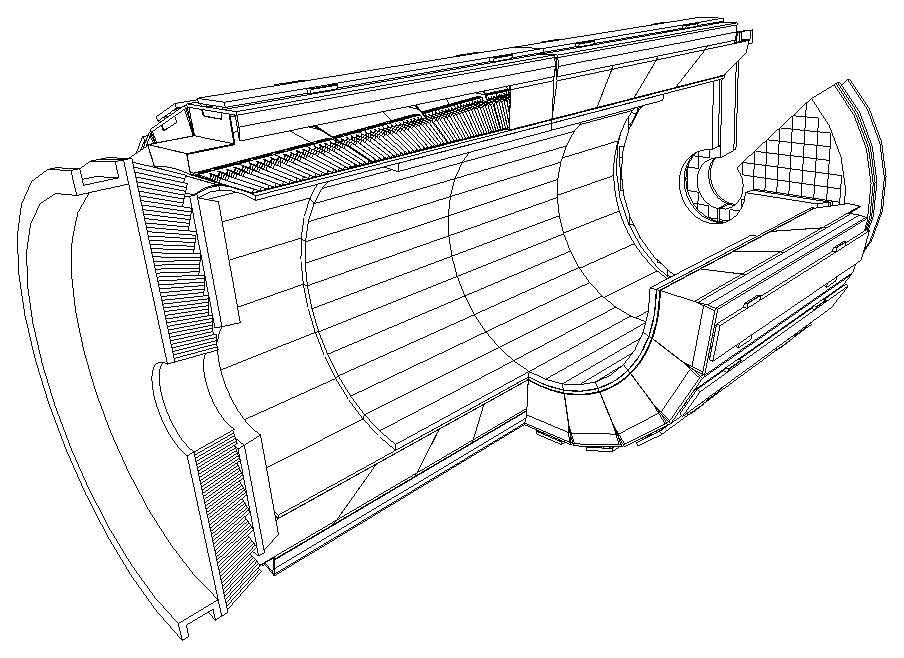
\includegraphics[scale=0.8]{cms-ecal}
\end{center}
\caption{Diagrama da seção eletromagnética do calorímetro do experimento CMS.}
\label{fig:cms-ecal}
\end{figure}

\subsubsection{Calorimetria hadrônica}
\index{Calorimetria!hadrônica}
\label{sec:calohad}

O chuveiro hadrônico é dominado por uma sucessão de interações inelásticas
deste tipo. Em altas energias, estas são caracterizadas pela produção de
partículas múltiplas e pela emissão de partículas originárias de decaimentos
nucleares do material excitado. Devido a freqüente geração de $\pi^{0}$'s
(diz-se ``pi-zeros'', ou seja, píons que não possuem carga elétrica),
chuveiros hadrônicos têm também componentes eletromagnéticas.

Quando um hádron altamente ener\-gé\-tico penetra num bloco de ma\-té\-ria,
ele, em algum ponto, interagi\-rá com algum nú\-cleo atômico. Neste processo,
mésons são usualmente gerados (píons, káons, etc.). Outra fração da energia
inicial da partícula é transferida para o núcleo com o qual o hádron
interagiu. Este núcleo excitado liberará esta energia emitindo um certo
nú\-mero de nú\-cleons (prótons ou nêutrons) e num estado posterior,
$\gamma$'s de baixa energia, perdendo sua energia cinética por ionização. As
partículas produzidas nesta reação (mésons, núcleons e $\gamma$'s), por sua
vez, podem perder sua energia cinética por ionização ou induzir novas reações
formando uma cascata ou chuveiro \cite{hadcal}.

Limites intrínsecos na resolução em energia de calorímetros hadrônicos são
\cite{hadcal}:

\begin{itemize}
  \item Uma componente $\pi^{0}$, flutuante dentre os chuveiros secundários, que
  interaja eletromagneticamente sem qualquer outra interação nuclear ($\pi^{0}
  \rightarrow \gamma\gamma$). A fração de $\pi^{0}$'s é dada por
  $\frac{\pi^{0}}{all} \approx 0,10 \log{E}$, $E$ em GeV. Chuveiros hadrônicos
  podem desenvolver uma componente eletromagnética dominante;

\item Uma boa parte da energia disponível é convertida em excitação e quebra
  de núcleos atômicos. Somente uma pequena fração desta energia aparecerá como
  sinal detetável, havendo largas flutuações evento-a-evento. Estas flutuações
  podem ser compensadas com a boa escolha dos materiais ativos e absorvedores
  do detetor;

\item Uma fração considerável da energia da partícula incidente é despendida
  em reações que não resultarão em sinal observável, tais como vazamento de
  energia em várias formas (evaporação ou quebra nuclear, excitação nuclear,
  etc.).
\end{itemize}

De forma contrária a chuveiros eletromagnéticos, que se desenvolvem num curto
espaço de tempo, chuveiros hadrônicos são caracterizada por diferentes escalas
de tempo. Os fenômenos mais lentos podem durar de centenas de nanossegundos a
um microssegundo.

Sumarizando:

\begin{enumerate}
\item Calorímetros são sensíveis a partículas neutras e carregadas;

\item Devido a diferenças na forma de deposição de energia das partículas, a
identificação de partículas com alta eficiência pode ser atingida usando-se
calorímetros;

\item Quanto maior a energia da partícula, mais acurado é o resultado. Isto não
acontece com outros tipos de detetores;

\item Para conter o desenvolvimento de cascatas dos objetos a serem medidos, a
profundidade dos calorímetros aumenta logaritmicamente com a energia, o que
permite o projeto de detetores mais compactos;

\item Não precisam de campos magnéticos (como os detetores de traços);

\item Podem ser segmentados, o que permite acurada medida da energia e a
visualização da tra\-je\-tó\-ria das par\-tí\-cu\-las;

\item Resposta rápida (melhor que 50 ns) pode ser atingida, o que é importante
num ambiente com alta taxa de eventos;

\item A informação de energia pode ser usada para filtrar eventos interessantes
com alta seletividade;
\end{enumerate}

\section{Sistemas de Filtragem}
\index{Sistemas de Filtragem}
\label{sec:trigger}

Os sinais detetados por calorimetria são normalmente utilizados como fonte de
discriminação rápida de eventos interessantes em experimentos modernos. Um
Sistema de Filtragem, ou \idxeng{Trigger}, é um conjunto de dispositivos,
normalmente uma combinação de componentes eletrônicos e computadores, provendo
um sinal rápido quando a física interessante acontece
\cite{bock:detector, cms-trigger, d0-trigger, d0-trigger2, hlt-tdr,
trig-review}. Tipicamente, um sistema de filtragem está associado a
experimentos com detetores e seus sinais ativam o sistema de gravação de
eventos para registrar parte ou a totalidade dos impulsos captados em mídia
permanente. As condições que levam o sistema de filtragem a produzir o sinal
de aceitação são comumente chamadas de
\idx{assinaturas do evento}. As condições podem ser tão simples quanto
identificar um traço gerado por uma partícula carregada passando por
cintiladores durante um período de tempo, ou tão complexos quanto o critério
de massa efetiva entre léptons identificados que devam satisfazer colisões de
altas energias.

Em muitos experimentos, a aquisição de dados, através do \idx{tempo morto} que
causa, é um fator crítico determinante, que limita as estatísticas e o
potencial físico. Um sistema de filtragem eficaz é então o ponto-chave para a
transmissão de dados que têm alta probabilidade de conter física de interesse
e rejeição, com base nas possibilidades de deteção, de todos ou da maioria dos
eventos que representem física ordinária e trivial. Claramente, não somente a
eletrônica e informática do sistema de filtragem são necessárias ao trabalho,
mas também os dados carregados pelo sistema de leitura do detetor, que provêem
as informações que serão averiguadas pelo primeiro.

Dependendo do acelerador utilizado, sistemas de filtragem podem ser chaveados
(e.g. por pacotes de partículas chegando ao ponto de colisão) ou
permanentemente ativados (como para o estudo de raios cósmicos). As
implementações podem ser síncronas ou operar em tempo real, ou ainda
se comporem de vários circuitos assíncronos operando paralelamente,
respeitando uma unidade de controle central (que também tem a função de
ressincronizar o sistema como um todo). As implementações nos dias de hoje, vão
desde simples portas E/OU até \idxeng{Field-Programmable Gate Arrays} ou
\idx{FPGA}'s. Os tempos de retardo dependem do volume dos dados a serem
analisados (e comumente da ocupação de recursos de processamento a que se
destinam). Algoritmos de filtragem também podem ter seu desempenho variando no
tempo, já que dependem da complexidade dos objetos em análise.

Em grandes experimentos, sistemas de filtragem são implementados em múltiplos
níveis, tipicamente consistindo de um primeiro nível síncrono, que identifica
candidatos a partir de um subconjunto dos dados colhidos pelos detetores,
reduzindo a taxa de eventos por algum fator. Subseqüentemente, os dados são
digitalmente transmitidos para \idx{bancos de memória} (do inglês
\idxeng{buffers}) e para um segundo nível de filtragem, normalmente assíncrono,
onde algoritmos mais complexos, baseados em um conjunto de dados mais
completo, conseguem reduzir novamente a taxa de eventos. Eventualmente,
depois de uma terceira ou quarta iteração, o evento é gravado em mídia
permanente.

\subsection{Sistemas de filtragem em experimentos modernos}

Um experimento em Física de Altas Energias como o DZERO \cite{d0}, localizado
no FermiLab, próximo a Chicago nos Estados Unidos, é um exemplo de um
experimento com um sistema de filtragem moderno. O cruzamento de pacotes de
prótons e anti-prótons que geram as colisões a serem estudadas ocorrem numa
taxa de 2,5 MHz (ou seja, 2,5 milhões de colisões por segundo). Cada colisão
poderá produzir um evento que possui 0,25 \eng{megabytes} em dados. Se a taxa
total fosse escrita em fitas magnéticas\footnote{Este tipo de tecnologia ainda
é atualmente utilizado para a armazenagem de grandes quantidades de dados ($>
10^{2} Terabytes$).}, assumindo um custo de 40 centavos de dólar por
\eng{Gigabyte}, o custo total seria de 10,5 milhões de dólares por ano. No 
entanto, a maior parte das colisões de pacotes contém interações elásticas ou
até mesmo nulas. Para tirar proveito desta natureza, o experimento DZERO
emprega um sistema de filtragem em múltiplos níveis para reduzir a taxa de
eventos registrada a 50 Hz, implicando em um custo aproximado de 75.000
dólares por ano em fitas magnéticas.

É claro que a economia em fitas magnéticas não é a única razão da existência
de um sistema de filtragem. Planejar e projetar um sistema de aquisição de
dados com uma taxa de dados de 600 \eng{gigabytes} por segundo seria
proibitivo economicamente, especialmente considerando-se o valor relativo dos
dados coletados. Os atuais programas de reconstrução de eventos também
consomem grande poder de processamento e, se a entrada puder ser sensivelmente
reduzida em volume, menor a quantidade de recursos computacionais serão
necessários para a análise \eng{offline}.

O enfoque usado para projetar e implementar um sistema de filtragem depende
fortemente do domínio do problema. Um experimento moderno em Física de Altas
Energias deve estar apto a responder a um novo evento, em geral, a cada
dezena ou dezenas de nanossegundos. O \idx{tamanho do evento} para grandes
experimentos (veja a Figura~\ref{fig:eventsize}) também tende a ser grande,
chegando a alguns \eng{megabyte} por evento em alguns dos experimentos do
\idx{LHC} (\idxeng{Large Hadron Collider}).

\begin{figure}
\begin{center}
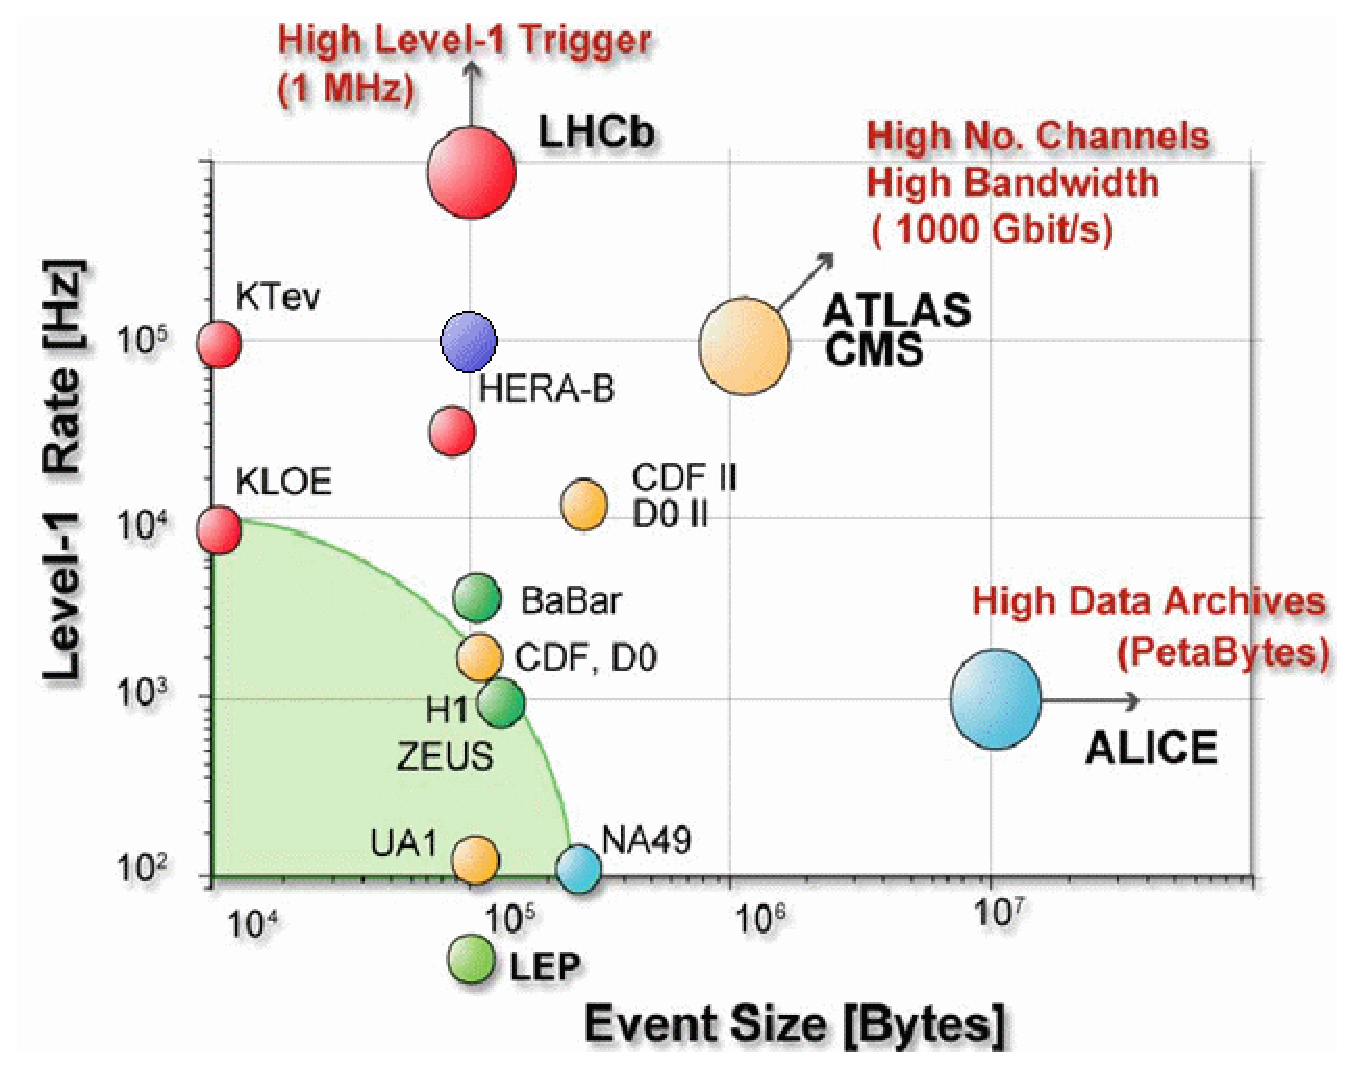
\includegraphics[scale=0.6]{eventsize}
\end{center}
\caption{O tamanho do evento \eng{versus} a taxa de produção em experimentos
atuais. Extraído de \cite{trig-review}.}
\label{fig:eventsize}
\end{figure}

Experimentos modernos usam um sistema de filtragem dividido em múltiplos
níveis para endereçar o problema das taxas de entrada. Os níveis mais baixos
implementam algoritmos simples e rápidos, normalmente usando FPGA's e
\eng{hardware} personalizado, que rejeitem os processos (\eng{background})
mais simples e abundantes. Os níveis mais altos são progressivamente mais
sofisticados e também requerem mais tempo para atingir níveis de rejeição
aceitáveis. Ademais, carregando uma menor quantidade ou melhor qualidade de
dados nos níveis iniciais de filtragem, estes experimentos conseguem reduzir o
fluxo de informação no sistema de leitura: tão logo um evento seja rejeitado,
seus dados são descartados.

Classicamente, o nível em \eng{hardware} é chamado de \idx{Primeiro Nível}. O
seguinte, composto de partes personalizadas em \eng{hardware} e computadores,
é chamado de \idx{Segundo Nível}. O último estágio, chamado de
\idx{Terceiro Nível}, composto normalmente de redes de computadores
tipo PC, realiza a classificação final. Comumente o segundo e terceiro níveis
de filtragem são conhecidos como \idx{Filtros de Alto Nível} ou
\idxeng{High-Level Triggers}, \idx{HLT}.

%% Hello emacs, this is -*- latex -*-
\typeout{ ====================================================================}
\typeout{ This is file atlas.tex, created at 13-Feb-2004 }
\typeout{ Maintained by Andre Rabello dos Anjos <Andre.dos.Anjos@cern.ch> }
\typeout{ ====================================================================}

\chapter{O Experimento ATLAS}
\label{chap:atlas}


%% Hello emacs, this is -*- latex -*-
\typeout{ ====================================================================}
\typeout{ This is file trigger.tex, created at 28-Feb-2004 }
\typeout{ Maintained by Andre dos Anjos <Andre.dos.Anjos@cern.ch> }
\typeout{ ====================================================================}

\chapter{O Sistema de Filtragem e Aquisi��o de dados do ATLAS}
\label{chap:trigger}

O \idx{sistema de filtragem} do experimento ATLAS tem o encargo de separar, em
tempo real, f�sica considerada ordin�ria para o experimento da rara f�sica de
interesse. A taxa de eventos produzida pelo LHC � da ordem 40 milh�es por
segundo, ou 40 MHz em bateladas que durar�o cerca de 10 horas (este per�odo �
comumente referido como \eng{run}). Cada evento poder� produzir uma colis�o
favor�vel a f�sica de interesse, embora a grande maioria, mais de 99,9999\%,
represente f�sica j� bastante estudada em experimentos anteriores ainda que a
luminosidade do sistema seja t�o elevada. Ademais, cada evento detetado pelo
ATLAS produzir� cerca de 1,5 Megabytes em dados, o que torna o problema da
filtragem bastante dif�cil, j� que o fluxo de dados que deve ser analisado por
base de tempo est� acima da capacidade de qualquer tecnologia de transporte
(de dados) atual.

Para o experimento ATLAS, o sistema de filtragem ser� constru�do em 3 n�veis
seq��nciais (veja a Figura~\ref{fig:trigger-sketch}). Cada n�vel que sucede
refina a decis�o do n�vel anterior atrav�s da aquisi��o de mais dados do
sistema de dete��o. O \idx{Primeiro N�vel} de filtragem (do ingl�s
\idxeng{First-Level Trigger}, L1) dever� reduzir a taxa de eventos do LHC para
cerca de 100 kHz apenas, atrav�s de t�cnicas simples de filtragem codificadas
em hardware personalizado. O \idx{Segundo N�vel} de filtragem (do ingl�s
\idxeng{Second-Level Trigger}, L2) reduzir� a taxa de sa�da do L1 para
aproximadamente 1 kHz utlizando aplica��es codificadas em software em
computadores do tipo PC. O \idx{Terceiro N�vel} de filtragem ou
\idx{Filtro de Eventos} (do ingl�s \idxeng{Event Filter}, EF) estar� baseado
na mesma tecnologia escolhida para o L2, reduzindo a taxa de entrada de
eventos para aproximadamente 100 Hz atrav�s de algoritmos de filtragem mais
eficientes por�m com menor desempenho.

\begin{figure}
\begin{center}
\includegraphics[angle=-90,scale=0.8]{trigger-sketch}
\end{center}
\caption{Vis�o funcional simplificada do sistema de filtragem do experimento
ATLAS.} 
\label{fig:trigger-sketch}
\end{figure}

\section{O Primeiro N�vel de Filtragem}

O Primeiro N�vel de Filtragem (L1) realiza uma sele��o inicial de candidatos �
f�sica de interesse baseado em informa��es com segmenta��o reduzida de um
subconjunto dos detetores do ATLAS, os calor�metros e o detetores de m�ons
\cite{l1-tdr}. M�ons com altos valores de \idx{momento transverso} ($p_T$) s�o
identificados � partir das c�maras de trigger conectadas ao Spectr�metro de
M�ons (veja a Se��o~\ref{sec:atlas-muon}) na regi�o do barril e da tampa. As
sele��es baseadas em calorimetria utilizam uma segmenta��o reduzida das se��es
e.m. e hadr�nica, no barril e na tampa. Os objetos procurados usando-se
calor�metros no L1 s�o el�trons com altos valores de $p_T$ e f�tons, jatos,
taus decaindo em cascatas hadr�nicas, grandes quantidades de energia faltante
ou energia transversa total. No caso da sele��o de el�trons e f�tons ou
h�drons e taus, isolamento em energia pode ser requisitado.

Para gerar os sinais de filtragem necess�rios ao L1, o sistema de leitura de
dados dos calor�metros � equipado com somadores r�pidos que aglomeram o sinal
de 1 ou mais c�lulas destes detetores para gerar macroc�lulas de filtragem
denominadas \idx{torres de filtragem} (do ingl�s \idxeng{Trigger Towers},
TT). O sistema de m�ons tamb�m possuem circuitos equivalentes que determinam a
ocorr�ncia de tra�os com altos valores de $p_T$. 

Os eventos selecionados pelo L1 s�o lidos pela eletr�nica prim�ria dos
detetores por \eng{drivers} denominados \idxeng{ReadOut Drivers} ou
\idx{ROD}'s. Cerca de 1.600 ROD's ser�o necess�rios para ler todos os dados do
detetor, ou seja, aproximadamente $10^7$ canais independentes. V�rios canais
de leitura s�o multiplexados em cada ROD. Bancos de mem�ria prim�rios,
chamados de \idxeng{derandomizers} garante um fluxo cont�nuo dos dados aos
ROD's apesar da irregularidade da aceita��o de eventos proporcionado pelo L1.

Os dados completos de eventos selecionados s�o guardados em bancos de mem�ria
denominados \idxeng{ReadOut Buffers} (ROB's) at� que o evento seja rejeitado
pelo L2 ou, no caso de ser aceito por este n�vel, at� que os dados sejam
transferidos para o terceiro n�vel de filtragem (EF). O processo de mover os
dados dos ROB's para of EF � chamado de \idx{constru��o do evento} (do ingl�s,
\idxeng{Event Building}, EB). Enquanto at� a fase de constru��o do evento os
dados est�o segmentados em ROB's, ap�s esta etapa o evento completo estar�
guardado em um �nico banco de mem�ria e acess�vel a um processador do EF.

\paragraph{Regi�es de Interesse} Al�m do disparo dado pelo L1 � eletr�nica de
leitura, este n�vel de filtragem deve enviar ao L2 um mapa dos objetos de
interesse encontrados no detetor durante a avalia��o do evento. Este mapa
indica, na precis�o do L1, as \idx{regi�es de interesse} no detetor (do ingl�s
\idxeng{Region of Interest}, RoI) que contribu�ram para a sele��o, os tipos
de objetos encontrados e o valor m�nimo (\eng{threshold}) de $p_T$ que
satisfazem. Informa��es de RoI's secund�rias (que n�o contribu�ram para a
decis�o do L1, mas que excitaram notavelmente o detetor) tamb�m podem ser
transmitidas ao L2, provendo uma maior capacidade de decis�o a este n�vel.

A Figura~\ref{fig:l1-context} mostra um diagrama do tipo ``caixa-preta''
indicando os sinais de entrada e sa�da do L1. A este sistema s�o injetados os
sinais provenientes da eletr�nica de leitura, dos sistemas de filtragem
diretamente acoplados aos detetores e do LHC (\eng{clock} de 40 MHz) e
colhidos sinais que s�o encaminhados para o L2, para a eletr�nica de aquisi��o
e para o sistema de monitora��o central.

\begin{figure}
\begin{center}
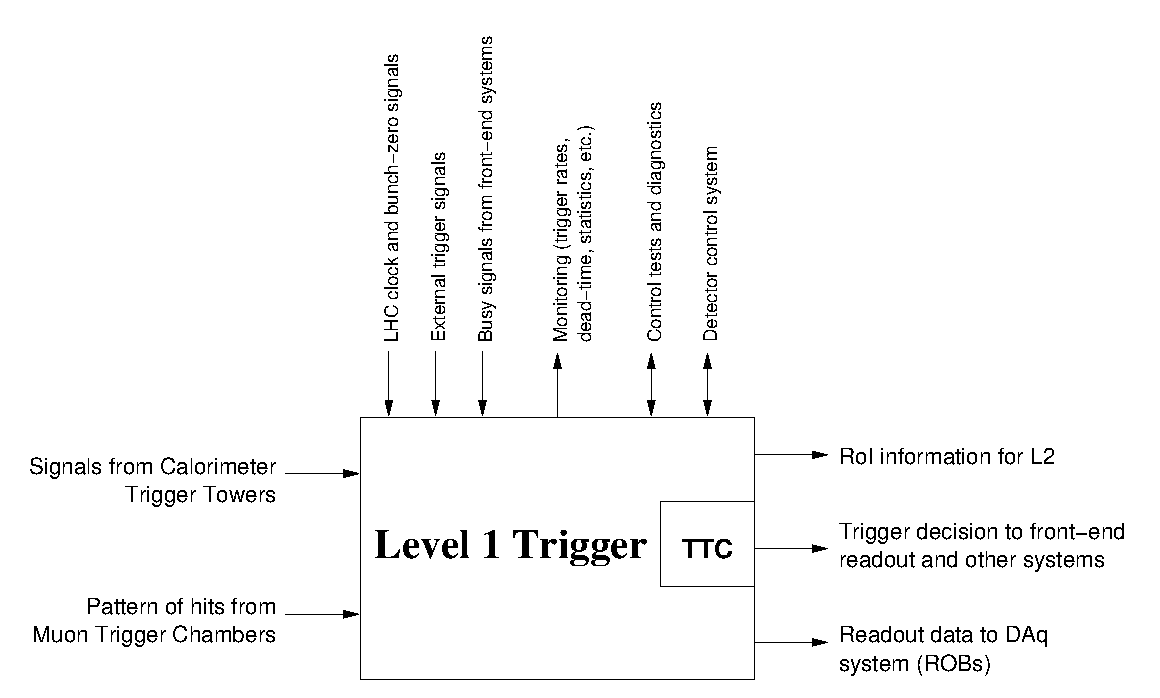
\includegraphics[scale=0.75,angle=-90]{l1-blackbox}
\end{center}
\caption{Diagrama simplificado dos sinais de entrada e sa�da do L1.}
\label{fig:l1-context}
\end{figure}

A Figura~\ref{fig:l1-functional} mostra um diagrama funcional simplificado do
L1. Nesta figura � poss�vel identificar processadores espec�ficos para os
sinais provenientes dos detetores. Um \idx{processador central de filtragem}
(marcado na figura como \idxeng{Central Trigger Processor}) � respons�vel pela
decis�o final e pela emiss�o do sinal para o L2 e para o sistema de
distribui��o de tempo, disparo e controle (indicado como \idxeng{Timming,
Trigger and Control distribution}, ou TTC), que gera finalmente o sinal para a
leitura dos dados do detetor. Dentre os componentes do TTC est� o
\idx{construtor de RoI's} (do ingl�s \idxeng{RoI Builder}, RoIB) que monta o
mapa de RoI's destacada pelo L1 e comunica, atrav�s de uma conex�o serial
r�pida tipo S-Link, estes dados ao L2.

\begin{figure}
\begin{center}
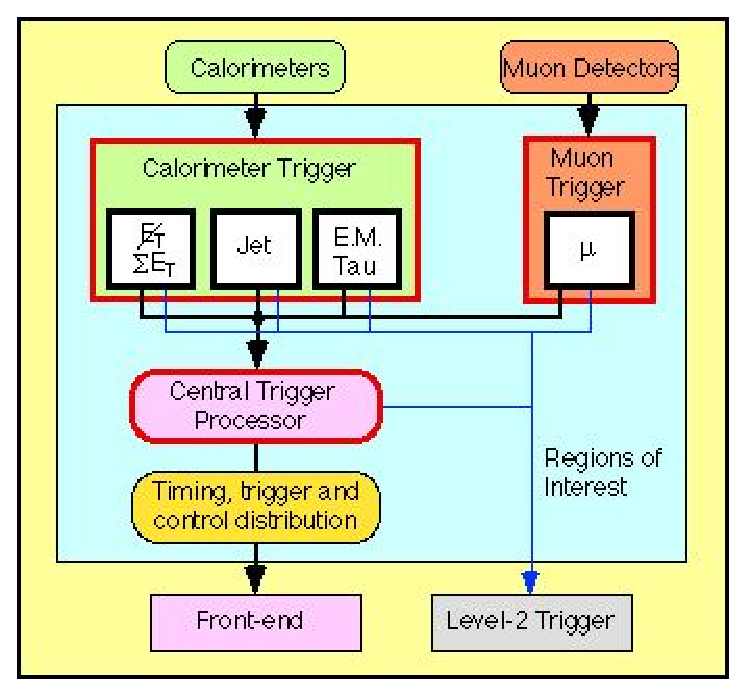
\includegraphics[scale=0.8]{l1-functional}
\end{center}
\caption{Diagrama em blocos indicando as principais fun��es do L1.}
\label{fig:l1-functional}
\end{figure}

\section{Os Altos N�veis de Filtragem e Aquisi��o de Dados}
\label{sec:hlt-daq}

O \idx{sistema de aquisi��o de dados} do ATLAS (do ingl�s \idxeng{Data
Acquisition System}, \idx{DAQ}) � composto pelos componentes que est�o
encarregados da transmiss�o e manipula��o dos dados produzidos pelo detetor. O
DAQ trabalha em coopera��o com os diversos n�veis de filtragem no experimento
de forma a garantir a corre��o dos dados transmitidos e a minimiza��o do
tempo-morto despendido na transfer�ncia de informa��o do sistema. A cadeia de
opera��o do DAQ � iniciada por um disparo do L1 para a leitura de dados
executada nos ROD's. Cada ROD � ligado, atrav�s de uma conex�o
S-Link\footnote{Conex�o ponto-a-ponto com taxa m�xima de transfer�ncia de 160
megabits por segundo.}, a somente um ROB. Cada ROB pode receber dados de um ou
no m�ximo 3 ROD's, dependendo da configura��o final do experimento.

Cabe aos \idx{Altos N�veis de Filtragem} (do ingl�s \idxeng{High-Level
Triggers}, \idx{HLT}), analisando de forma �tima os dados presentes nos ROB's,
decidir, disparando mais uma vez o DAQ sobre o futuro de cada evento aceito
pelo L1. O conjunto HLT/DAQ funcionar� harmoniosamente sobre uma mesma base
computacional e utilizando o mesmo conjunto de ferramentas para a codifica��o,
an�lise e depura��o de problemas que possam ocorrer. Por esta raz�o, o HLT/DAQ
� considerado um macro-sistema do experimento. O sistema HLT/DAQ pode ser
subdividido em 4 partes:

\begin{itemize}
\item \textbf{\idx{fluxo de dados} ou \idxeng{Dataflow}}: este sistema �
respons�vel por receber os dados do detetor, servir um subconjunto destes
dados ao HLT e transportar os dados de eventos selecionados em �ltima
inst�ncia para armazenagem em m�dia permanente;

\item \textbf{\idx{filtros de alto n�vel} ou \idx{HLT}}: s�o respons�veis pela
sele��o de eventos ap�s o L1, envolvendo a redu��o da taxa de eventos e a
classifica��o de todos os eventos aceitos;

\item \textbf{\idxeng{online}}: � respons�vel por todos os aspectos de
opera��o e controle durante a aquisi��o de dados do experimento e durante
\eng{runs} de teste e calibra��o;

\item \textbf{\idx{sistema de controle do detetor} ou \idxeng{Detector Control
System}, \idx{DCS}}: respons�vel pela opera��o coerente e segura (no que tange
radia��o, controle de altas tens�es, etc.) do detetor ATLAS e pelo
interfaceamento com sistemas externos e servi�os incluindo o acelerador LHC.
\end{itemize}

\typeout{ *************** End of file trigger.tex *************** }

%% Hello emacs, this is -*- latex -*-
\typeout{ ====================================================================}
\typeout{ This is file baseline.tex, created at 18-Aug-2006 }
\typeout{ Maintained by Andre Anjos <Andre.dos.Anjos@cern.ch> }
\typeout{ ====================================================================}

\chapter{Filtragem baseada em calorimetria no experimento ATLAS}
\label{chap:baseline}

Sistemas de calorimetria são habitualmente construídos com forma e leitura
segmentada de maneira que possam ser usados diretamente na dete\-ção de
par\-tí\-culas. Isto é possível uma vez que muitos processos interessantes são
distinguíveis pela forma com que depositam energia à medida que interagem com
estes detetores, tanto de forma radial quanto longitudinal
\cite{wigmans-book}. Cada segmento ou célula de um calorímetro contém a
informação de energia depositada por uma par\-tí\-cula ou conjunto de
par\-tí\-culas que interagiu com o detetor naquela área espe\-cí\-fica. A
seg\-men\-ta\-ção destes instrumentos dependerá da Física do experimento e
também, normalmente, do eixo de dispersão das partículas de interesse.

Algoritmos de dete\-ção são normalmente concebidos por especialistas em
Calorimetria que compreendam os diferentes perfis de intera\-ção para a
Fí\-sica de interesse. O primeiro passo é definir um processo de redu\-ção de
dimensionalidade, de acordo com os processos que se deseja detetar, ainda que
levando-se em consideração à velocidade requerida na deteção. Quanto menor o
tempo disponível à deteção, maior a compressão a ser realizada de forma a
simplificar este processo. Este pré-processamento para a compressão dos dados
ou Extração de Características (do inglês, \eng{Feature Extraction} ou FEx) é,
em geral, feito com perda de informação do perfil de deposição, mas de forma a
manter as principais características do objeto que se deseja detetar. Em
seguida, tendo por base simulações ou dados reais da Física de interesse,
define-se um conjunto de cortes por métodos com conhecimento da informação
\eng{a priori} que maximizem a probabilidade de deteção das partículas
interessantes.

O Sistema de Filtragem \eng{online} do experimento ATLAS deverá prover uma
seleção de eventos muito eficiente e desprovida de tendências, mantendo o
potencial de descoberta do detetor. Deve ser extremamente flexível, de forma a
operar no ambiente desafiador do LHC, com até 23 colisões inelásticas por
interação, 14~TeV de energia no centro de massa e apenas 25~ns (40~MHz) entre
colisões sucessivas. Além disso, deve prover critérios de seleção robustos e,
onde possível, redundantes. É altamente desejável a rejeição de canais
ruidosos, não interessantes ou falsos o mais rápido possível, de forma a
otimizar o uso dos recursos computacionais disponíveis.

Para trazer uma eficiência compatível com este árduo ambiente, o Sistema de
Filtragem fará uso de um enfoque baseado na \textbf{inclusão} para a seleção
\eng{online}, garantindo assim um conjunto de \eng{triggers} ótimo para a nova
Física. O critério da inclusão tem por objetivo selecionar um conjunto de
fenômenos físicos baseados em características comuns entre eles, que ainda
sejam claramente distinguíveis dentro do ruidoso ambiente produzido pelo
acelerador. Com este objetivo, o Sistema de Filtragem estará sendo disparado
para eventos que contenham assinaturas baseadas em objetos simples ou duplos
com alto valor de momento transverso. Neste contexto, objetos com alto valor
de momento transverso são, entre outros, \eng{léptons} com carga e com momento
transverso acima de $\sim$10 GeV \cite{hlt-tdr}.

Neste capítulo, fazemos uma análise do processo de filtragem de elétrons a ser
conduzido no Sistema de Filtragem do experimento ATLAS. Como em muitos outros
experimentos em Física de Altas Energias \cite{abolins-calor-2000,
monteiro-calor-1999}, este sistema é seccionado em níveis que realizam o
processo de filtragem em passos com complexidade e tempo de execução
crescentes. O primeiro dos níveis é normalmente implementado em
\eng{hardware}, para atender as demandas de tempo do feixe, enquanto que os
demais em \eng{software}, maximizando a flexibilidade. Em particular, atenção
será dada à definição do funcionamento do Primeiro e Nível de Filtragem (LVL1)
com relação a deteção de elétrons e, em seguida, o sistema desenvolvido
atualmente para o LVL2. Finalmente, uma caracterização dos dados disponíveis
segundo as premissas desenvolvidas neste capítulo é estabelecida como base de
comparação ao restando do trabalho.

\section{Objetos de interesse e RoI's}

Foi visto no Capítulo~\ref{chap:trigger} que o Primeiro Nível de Filtragem do
ATLAS define, para objetos encontrados seja nos Calorímetros ou nos Detetores
de Múons, regiões de interesse onde objetos relevantes tenham sido
observados. Para cada objeto interessante, a região aproximada de interação do
objeto com o detetor é anotada e repassada aos demais níveis de filtragem, no
caso da aprovação do evento pelo LVL1. Este processo define as Regiões de
Interesse ou RoI's, que guiarão o processo de seleção nos Altos Níveis de
Filtragem (do inglês, \eng{High-Level Triggers} ou HLT).

De fato, dadas as condições do feixe provido pelo LHC, múltiplos objetos
poderão ser detetados a cada evento. Porém, quando um ou mais objetos
detetados ativam a aceitação do evento, o LVL1 marca o dado de forma especial,
distinguindo este objeto como primário, em contraste com aqueles que também
foram detetados, mas não fizeram objeto da aceitação deste nível de
filtragem. O processo de deteção no LVL2 começa por uma confirmação dos
objetos primários detetados pelo LVL1, utilizando-se da granularidade
completada do detetor ao redor da RoI. Em seguida, o processo de filtragem
poderá, eventualmente, ser refinado ainda neste nível de filtragem ou mais a
frente, no EF, complementando-se a análise com base em RoIs secundárias. Este
sistema de filtragem \eng{online} baseado em RoIs é um elemento de
diferenciação do experimento ATLAS \cite{atlas-tp}, sendo esta a primeira vez
que é implementado em um ambiente em Física de Altas Energias.

A Tabela~\ref{tab:l1-rates} apresenta as taxas (simuladas) para as diferentes
assinaturas de interesse, ou conjuntos de objetos primários, que serão
entregues pelo LVL1~\cite{hlt-tdr} ao HLT, encabeçados pelo LVL2, para a
luminosidade inicial de $2\times10^{33}cm^{-2}s^{-1}$. Este valor de
luminosidade está cerca de uma ordem de magnitude abaixo do valor final de
operação do LHC, de $\approx 10^{34}cm^{-2}s^{-1}$. Com o aumento da
luminosidade do feixe, a relação entre as taxas ou até o tipo das assinaturas
nesta tabela sofrerá alterações tendo em vista a mudança na probabilidade de
ocorrência de fenômenos mais raros.

\begin{table}
\caption{Taxas de saídas para as assinaturas reconhecidas pelo LVL1,
para a luminosidade de pico inicial de $2\times10^{33}cm^{-2}s^{-1}$. Dados
baseados em uma simulação do LVL1.}
\label{tab:l1-rates}
\begin{center}
\begin{sideways}
\begin{tabular}{|l|l|r|}
\hline
\textbf{Assinatura do LVL1} & \textbf{Codinome} & \textbf{Taxa (kHz)} \\ \hline
e.m., 25 GeV, com isolamento & \texttt{EM25i} & 12 \\ \hline
2 $\times$ e.m., 15 GeV, com isolamento & \texttt{2EM15i} & 4 \\ \hline
Múon, 20 GeV & \texttt{MU20} & 0.8 \\ \hline
2 $\times$ múon, 6 GeV & \texttt{2MU6} & 0.2 \\ \hline
Jato, 200 GeV & \texttt{J200} & 0.2 \\ \hline
3 $\times$ jato, 90 GeV & \texttt{3J90} & 0.2 \\ \hline
4 $\times$ jato, 65 GeV & \texttt{4J65} & 0.2 \\ \hline
Jato, 60 GeV $+$ \textit{Missing Energy}, 60 GeV & \texttt{J60} $+$
\texttt{XE60} & 0.4 \\ \hline
$\tau$, 25 GeV, com isolamento $+$ \textit{Missing Energy}, 30 GeV &
\texttt{TAU25i} $+$ \texttt{XE30} & 2 \\
\hline
Múon, 10 GeV $+$ e.m., 15 GeV, com isolamento & \texttt{MU10} $+$ \texttt{EM15i} & 0.1 \\ \hline
Outros disparos (pré-escalonados, aleatórios, calibração, monitoração) & -- & 5 \\
\hline
Total & -- & $\sim$25 \\ \hline
\end{tabular}
\end{sideways}
\end{center}
\end{table}

Nota-se que, aproximadamente, 16 dos 25 kHz (i.e. $\sim$65\% das assinaturas)
entregues pelo LVL1 conterão objetos tipo e.m.. Estes objetos são assim
classificados por representarem elétrons \textbf{ou} fótons, que interagem com
os detetores a partir de interações eletromagnéticas em vez das componentes
hadrônicas presentes em outros casos. Em algumas das assinaturas, exige-se que
o objeto seja \emph{isolado}. Isto quer dizer que a quantidade de energia no
centro do objeto deverá manter uma razão mínima com relação a energia
depositada em sua periferia, como ficará claro mais a frente.

\section{Análise do sistema de filtragem com relação à Física}

A Figura~\ref{fig:trigger-physics} apresenta um diagrama esquemático que
despreza as interfaces em \eng{hardware} propostas pela construção do Sistema
de Filtragem e tenta enfocar melhor o problema do ponto de vista da análise
dos canais físicos. De cima para baixo, indica-se o tráfego de mensagens até a
completa aceitação de um evento por parte do Sistema de Filtragem.

\begin{figure}
\begin{center}
\includegraphics[scale=0.9]{trigger-physics}
\end{center}
\caption{Diagrama esquemático do Sistema de Filtragem do Experimento ATLAS
segundo suas funções de filtragem.}
\label{fig:trigger-physics}
\end{figure}

O processamento começa à medida que o LVL1 recebe o sinal do LHC acusando o
iminente cruzamento de pacotes (do inglês \eng{Bunch Crossing}) no ponto de
impacto (mensagem \ding{182}). Uma janela de aquisição de alguns nanossegundos
fará com que o Sistema de Leitura do LVL1 registre o evento (mensagem
\ding{183}). Os sistemas de pré-processamento são ativados em seguida.

No caso dos Calorímetros, somadores rápidos \cite{seixas:adder} agrupam as
informações das células dos calorímetros e.m. e hadrônicos, formando, para
cada seção, uma matriz de dados com granularidade reduzida
\cite{l1-tdr}. Estas macro-células ou ``torres'' de filtragem (do inglês,
\eng{Trigger Towers}, ou TT) agrupam os dados formando elementos com tamanho
igual a $0,1\times0,1$ no plano $\eta\times\phi$. Estes dois planos com
granularidade minimizada são varridos pelos diversos processadores do LVL1 e
os objetos de interesse, ou seja RoI's, localizados no detetor. Um processo
análogo é conduzido tendo por base os detetores de múons, com o objetivo de
encontrar objetos deste tipo (mensagem \ding{184}).

No final do processamento pelo LVL1, rapidamente depois da colisão, e no caso
de tratar de um evento interessante, uma mensagem contendo a localização dos
objetos encontrados por este nível de filtragem e variáveis indicando as
assinaturas pelo qual o evento foi aprovado, é repassada ao LVL2
(mensagem \ding{185}). Esta mensagem é chamada de Resultado do LVL1 (do inglês
\eng{LVL1 Result}) ou L1R, como visto na Seção~\ref{sec:lvl2arch}. Nota-se que
o L1R pode conter múltiplas assinaturas em um único evento, no caso deste
conter elementos que confirmem mais de uma das linhas da
Tabela~\ref{tab:l1-rates}. Ademais, múltiplas RoI's secundárias podem estar
presentes na lista de objetos na mensagem. Em paralelo ao envio da mensagem em
direção ao LVL2, o LVL1 indica ao sistema de aquisição de dados (marcado na
figura como \eng{Read Out}) que carregue todos os dados do detetor em seus
\eng{buffers}.

O processamento no LVL2 é seqüencial. Ao receber um L1R, o Coordenador de
Execução do LVL2 (do inglês, \eng{Steering}) chamará um algoritmo de filtragem
para a confirmação do disparo do LVL1. O algoritmo em questão poderá
transferir, do sistema de leitura do detetor, a quantidade de dados que achar
necessária, ao redor da RoI, de forma a processá-la (mensagem \ding{186}). Se
não for possível rejeitar a assinatura do LVL1, o \eng{Steering} poderá chamar
mais e mais algoritmos até que o evento seja rejeitado ou definitivamente
aprovado ao Terceiro Nível de Filtragem ou Filtro de Eventos (do inglês
\eng{Event Filter} ou EF). Neste último caso, de forma equivalente à relação
entre o LVL1 e o LVL2, o LVL2 enviará um sumário indicando a razão da
aceitação do evento ao EF (mensagem \ding{187}). Este sumário contém valores
refinados de energia, momento e localização dos objetos explorados no contexto
LVL2. Analogamente ao resultado do LVL1, o resultado do LVL2 é chamado L2R (do
inglês {LVL2 Result}). Espera-se que o LVL2 atinja uma redução da taxa de
eventos de aproximadamente 25 vezes, de forma que o EF possa operar a uma taxa
de apenas alguns (1 ou 2)~kHz. O tempo médio de processamento para o LVL2 deve
estar na ordem dos 10~ms e para o EF, na ordem de alguns segundos, levando-se
em consideração o número de processadores disponíveis nestes níveis de
filtragem. No caso do evento ser aprovado pelo EF, é armazenado em mídia
permanente (mensagem
\ding{188}).

Os tempos de processamento-alvos representam a média de processamento por
evento. De fato, espera-se que eventos de interesse utilizem mais tempo de
processamento, enquanto que eventos pouco ou nada interessantes sejam
rapidamente descartados. Neste contexto, entende-se que, quanto menor o tempo
necessário e maior a qualidade da deteção dos diversos componentes do sistema
de filtragem, mais tempo computacional será despendido com a Física de
interesse e menos recursos com eventos que representem Física ordinária.

Diferentemente do LVL2, a análise no EF começa com 100\% dos dados do evento e
os resultados dos nível precedentes (L1R e L2R) já disponíveis na
memória. Neste nível de filtragem, correlações mais complexas podem ser feitas
entre as diferentes RoI's, e uma análise mais depurada do evento poderá ser
conduzida. Por exemplo, é possível fazer uso das RoI's secundárias para
atingir maior redução da taxa de eventos a serem registrados em mídia
permanente. Se aprovado, o evento é guardado, devidamente ``etiquetado'' e
repassado às fazendas (\eng{farms}) de processamento \eng{offline} para
posterior reconstrução.

\section{Deteção de elétrons baseada em calorimetria}
\label{sec:e-detection}

O \eng{trigger} de elétrons ou fótons para o ATLAS conterá forte contaminação
de jatos com componentes hadrônicas, que formam o ruído de fundo na deteção de
elétrons \cite{nevski-calor-1992}. Estima-se que o ruído de contaminação
original esteja na ordem de $10^6$. O LVL1 do ATLAS poderá excluir grande
parte dos jatos QCD, se as conversões hadrônicas forem importantes neste
objeto, e apenas observando a quantidade de energia hadrônica depositada na
seção de mesmo nome dos calorímetros, mas terá pouca eficiência em conversões
com menos componentes hadrônicas. Estima-se em
\cite{daqnote00-02}, que a cada 25.000 objetos do tipo e.m., aprovados pelo
LVL1, apenas 1 será um elétron ou fóton verdadeiro. Somente no LVL2, o Sistema
de Filtragem, disporá do tempo e da completa granularidade do detetor para
executar uma seleção mais criteriosa, refinando a decisão obtida no LVL1
\cite{hlt-tdr} (mas originalmente discutida em \cite{ellis-calor-1992}). O
algoritmo de calorimetria também refina a posição do objeto originalmente
determinada pelo LVL1, de forma que algoritmos de deteção de traços,
reconhecidamente menos eficientes, possam reduzir sua área de procura. Por
estas razões, a correta identificação de elétrons é de suma importância para o
experimento.

A Figura~\ref{fig:e-shower} mostra a interação de um elétron com um detetor de
traços (\eng{Cloud Chambers}) e absorvedores de chumbo. Nesta figura, é
possível observar a formação de um chuveiro de partículas que diverge,
aproximadamente de forma isotrópica, do eixo de penetração do elétron. No caso
de elétrons \cite{wigmans-book}, a dispersão é menor que no caso de jatos de
partículas, já que há uma grande probabilidade de espalhamento múltiplo (do
inglês \eng{Multiple Scattering}) causado pelas componentes hadrônicas do
conjunto de partículas. A distância de penetração é diretamente proporcional à
energia do objeto em análise \cite{leo, knoll}, ainda que, para os mesmos
valores energéticos, jatos tendam a penetrar mais profundamente nos
dispositivos.

\begin{figure}
\begin{center}
\includegraphics[scale=0.4]{e-cloud-chamber}
\end{center}
\caption{Interação de um elétron com um detetor de traços com absorvedores em
chumbo.} 
\label{fig:e-shower}
\end{figure}

%%CONSEGUIR FOTO DE UMA ROI COM O DÊNIS: ELECTRON, JET?

A deteção de elétrons beneficia-se deste conhecimento básico para
distingui-los de sua contaminação natural de jatos (e píons). Numa primeira
fase, chamada de Extração de Características, avalia-se, para uma região do
detetor, normalmente centralizada em um ponto pré-determinado, um conjunto de
valores que representem, o melhor possível, os perfis de deposição lateral (ou
radial) do objeto sendo estudado e sua penetração no aparato. Este processo
comprime\footnote{Para os fins deste trabalho define-se ``compressão'' ou
compactação a técnica pelo qual reduz-se a dimensionalidade de um sinal em um
espaço bem definido, preservando ou tentando preservar a informação relevante
que caracteriza este sinal de interesse. A transformação do espaço original
para o espaço ``comprimido'' é irreversível, salvo onde especificado.} a
informação de entrada, que normalmente possui dimensionalidade bastante
elevada (O(100)-O(1000)), para um conjunto pequeno (O(10)) de variáveis que
possam ser analisadas mais facilmente.

A questão da dimensionalidade da entrada está intimamente correlacionada com a
capacidade discriminatória do calorímetro. Quanto mais granular, maior
precisão pode ser obtida na definição de pontos de impacto e deteção de
partículas. O revés é o custo - detetores multi-segmentados são mais difíceis
e custosos de serem construídos.

No caso do experimento ATLAS (veja a Seção~\ref{sec:atlas-calo} para mais
detalhes), os calorímetros são segmentados em diversas camadas, e, camada a
camada, granularizados em células de deposição energética. A granularidade
varia camada a camada, pois cada uma delas possui um objetivo distinto de
emprego: as camadas iniciais têm por objetivo a discriminação de elétrons e
fótons e estimativa de posicionamento, as mais traseiras a deteção de
hádrons. As camadas da seção e.m. têm profundidade variante, sendo que a
segunda (EM2, a contar do zero, ou seja o pré-irradiador), tem a maior
profundidade de todas, ocupando mais de 80\% do volume total desta seção.

Para elétrons com valores energéticos até algumas dezenas de
gigaelétron-volts, espera-se que a maior parte da energia do objeto esteja
depositada nesta camada. A granularidade é bastante regular, tanto ao longo do
eixo $\eta$ quanto ao longo de $\phi$, como é possível observar na
Tabela~\ref{tab:lar}. Esta tabela também mostra o fator de compressão (ou
tamanho da torre de filtragem) $N_{\eta} \times N_{\phi}$ aplicado ao processo
de agrupamento necessário ao pré-processamento antes da análise feita pelo
LVL1.

A seção hadrônica do calorímetro é bastante menos granular. O tamanho padrão
da célula ($0,1\times0,1$ no espaço $\eta\times\phi$) foi otimizado para
detetar hádrons. Esta classe de partículas penetra mais profundamente na
matéria e desenvolve complexas cascatas ao longo da penetração, normalmente
pouco interessantes. Entretanto, devem estar contidas no espaço do detetor. O
agrupamento padrão (torre de filtragem) para o LVL1 é de $2\times2$ células.

A Figura~\ref{fig:e-jet-deposit} mostra histogramas da relação da deposição
energética na seção hadrônica e a energia total do objeto considerando-se uma
área $0,4\times0,4$ no plano $\eta\times\phi$. Os eventos considerados são
simulações de elétrons e jatos cobrindo um campo energético de algumas dezenas
de GeV até 90 GeV interagindo com os calorímetros do ATLAS. Os eventos
selecionados passaram uma simulação realística do LVL1 e portanto representam,
todos, eventos que seriam classificados como elétrons por este nível de
filtragem. Observa-se que para jatos há uma probabilidade maior de depósito na
seção hadrônica que na seção e.m..

\begin{figure}
\begin{center}
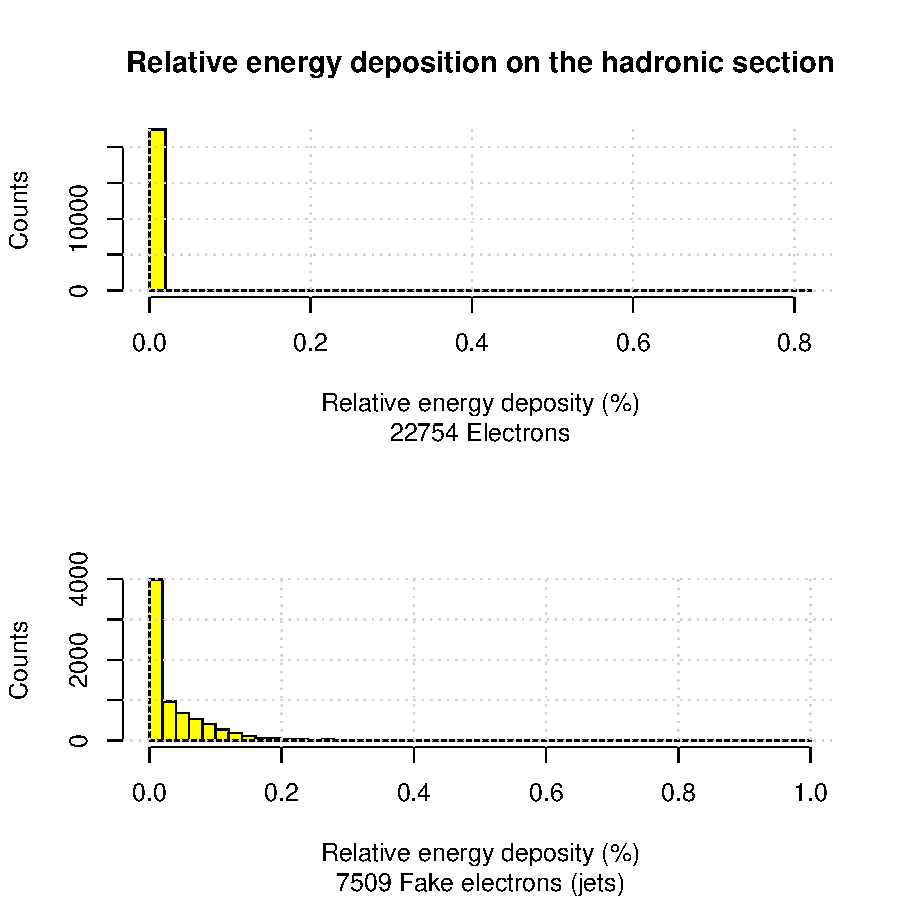
\includegraphics[scale=0.95]{em-had-percent}
\end{center}
\caption{Exemplo da relação de deposição energética na seção hadrônica e
energia total para elétrons (topo) e jatos (baixo).}
\label{fig:e-jet-deposit}
\end{figure}

Em seguida, aplica-se a discriminação da Física de interesse. Tipicamente
\cite{nevski-calor-1992, guida-calor-1992, palutan-calor-2000}, a deteção é
realizada por meio da definição de patamares de separação (também ditos
\emph{cortes}) com informação \emph{a priori}. Este trabalho é normalmente
realizado por um físico experiente, de acordo com os canais físicos de maior
interesse para o experimento.

%É importante salientar que o melhor classificador baseado em cortes com
%informação \emph{a priori} também pode ser atingido iterativamente através de
%utilização de discriminadores lineares \cite{haykin-adaptative}, opcionalmente
%com atribuição de pesos para cada classe de partículas, definindo importâncias
%diferentes aos diferentes tipos de objetos estudados.

\section{Deteção de elétrons no LVL2}
\label{sec:lvl2-detect-electron}

O LVL1 (Seção~\ref{sec:lvl1}) executa seu procedimento de filtragem procurando
elementos nos calorímetros e detetores de múons que obedeçam a certos
critérios de classificação. A Tabela~\ref{tab:l1-rates}, mostrada
anteriormente, indica os principais objetos de interesse. No caso de objetos
e.m. (elétrons e fótons), o algoritmo pode ser resumido da seguinte forma:

\begin{enumerate}
\item Os sinais analógicos provenientes das células do detetor são agrupados
em macro-células chamadas Torres de Filtragem (do inglês \eng{Trigger Towers},
TT). A taxa de agrupamento não é uniforme, mas, em geral, forma TT's com
$0,1\times0,1$ no plano $\eta\times\phi$ para a seção eletromagnética do
calorímetro e $0,2\times0,2$ na seção hadrônica;

\item Os sinais somados das TT's são disponibilizados para a
lógica de leitura do LVL1;

\item Processadores especializados (4 no total) cobrem diferentes áreas do
detetor e utilizam um algoritmo de agrupamento, baseado em uma janela
deslizante \cite{l1-tdr} cobrindo uma região de $4\times4$ TT's (16 no
total), aqui resumido:

\begin{enumerate}
\item Se o núcleo de $2\times2$ TT's contiver energia maior que a
periferia, para um determinado patamar programável, um candidato a RoI é
definido;

\item Em seguida, somam-se, duas a duas, as energias transversas das TT's do
núcleo de $2\times2$ TT's e utiliza-se a maior das somas em uma comparação com
um patamar de energia EM;

\item Caso passe este critério, a energia na periferia da RoI-candidata é
verificada para assegurar o isolamento do objeto; 

\item O último critério é o isolamento hadrônico, onde o LVL1 verifica se não
há grande depósito de energia (transversa) na seção hadrônica.
\end{enumerate}  

No caso de atender a todos os pré-requisitos, o objeto candidato é promovido a
uma RoI tipo e.m.. Este algoritmo está representado na
Figura~\ref{fig:l1-calo}.
\end{enumerate}

\begin{figure}
\begin{center}
\includegraphics[scale=0.78]{l1-calo}
\end{center}
\caption{Representação gráfica do algoritmo de deteção de objetos e.m. no LVL1.}
\label{fig:l1-calo}
\end{figure}

Os diversos sub-módulos do LVL1 irão detetar e pré-classificar os elementos de
interesse para jatos, múons e energia faltante. Em seguida:

\begin{enumerate}
\item Os objetos detetados e seus pontos \textbf{centrais} de impacto
estimados no plano $\eta\times\phi$, ou seja, as RoIs, são encaminhados ao
Processador Central do Sistema de Filtragem do LVL1 (do inglês \eng{Central
Trigger Processor}, CTP) e uma decisão é feita levando-se em consideração as
assinaturas de interesse e resultados dos processamentos de outros módulos
(jatos, energia faltante e múons). A decisão de aprovar um evento é tomada
baseando-se em RoI's de acordo com critérios de preferência estipulados \eng{a
priori}. As RoI's que são utilizadas para a decisão de aprovação são rotuladas
``primárias'' ao passo que as demais, ``secundárias'';

\item Um sumário do resultado e das RoI's encontradas, já rotuladas (primárias
e secundárias) é repassado, através do \eng{RoI Builder} ao LVL2.
\end{enumerate}

A primeira vez onde o evento será analisado tendo por base a granularidade
máxima do detetor é no Segundo Nível de Filtragem do experimento ATLAS. O
objetivo deste nível de filtragem, de uma forma geral, é a confirmação das
informações do LVL1 e eventual depuração e extensão. Aproveitando-se de toda a
granularidade disponibilizada pelo sistema de leitura do detetor, o LVL2
começa analisando o evento através das RoI's classificadas como primárias pelo
LVL1.

Ao receber as informações das RoI's o \eng{Steering} ativará o passo de
decodificação do resultado do LVL1 e, em seguida, selecionará a próxima fase
de análise, que dependerá diretamente do tipo das RoI's primárias do
evento. No caso de RoI's do tipo e.m., um algoritmo de deteção de elétrons (e
fótons) será ativado.

\section{Deteção de elétrons no LVL2 do ATLAS}
\label{sec:classic-detection}

Como discutido anteriormente, na Seção~\ref{sec:e-detection}, o processo de
deteção veloz baseado em calorimetria pode ser sub-dividido nas seguintes partes:

\begin{enumerate}
\item Compactação do sinal de entrada;
\item Deteção da Física de interesse baseada no espaço comprimido.
\end{enumerate}

Para o ATLAS, a fase de compactação irá mapear o espaço de entrada definido
pelas células da RoI sendo tratada em 4 variáveis com alto poder
discriminatório, baseado na percepção da Física de interesse e da contaminação
esperada. No caso de elétrons, espera-se que haja forte contaminação de jatos
com muitas componentes e.m.. Desta forma, a compactação da informação de entrada
tentará realçar informações como a dispersão do objeto na RoI ou a
profundidade de interação do objeto com as diversas camadas do detetor.

O nome do algoritmo usado para a FEx de RoI's primárias tipo e.m. é
\emph{T2Calo}, uma abreviação composta das palavras \eng{Trigger}, LVL2 e
Calorimetria. As variáveis extraídas do \eng{cluster} definido pela RoI do
LVL1, por este algoritmo, estão descritas a seguir. Cada uma destas variáveis
define uma etapa ou mais etapas do processamento do T2Calo que está
esquematizada nas figuras correspondentes:

\begin{enumerate}
\item \textbf{Energia do núcleo e.m.}, Figura~\ref{fig:t2calo-1}: O
primeiro passo do algoritmo é um refinamento do centro da RoI. Isto é feito
encontrando-se o pico de deposi\-ção ener\-gé\-tica na segunda camada da
se\-ção eletroma\-gné\-tica do calo\-rí\-metro, que é tam\-bém a mais profunda
desta se\-ção (veja uma discus\-são mais detalhada da geometria do detetor na
Seção~\ref{sec:atlas-calo}). O valor do centro da cé\-lula é tomado como uma
nova estimativa de posicionamento da RoI e será utilizado para os cál\-culos
seguintes.

Em seguida, ainda utilizando-se dos dados da segunda camada e.m., calcula-se a
soma dos valores de deposição energética numa região de tamanho
$\Delta_\eta=0,075\times\Delta_\phi=0,175$ e numa região de tamanho
$\Delta_\eta=0,175\times\Delta_\phi=0,175$, ao redor do centro de impacto
encontrado anteriormente. De posse destes valores, a primeira característica
será extraída:

\begin{equation}
\rcore \text{ ou } R_\text{core} = \frac{\text{Energia}^{e.m.2}_{\Delta_\eta=0,075\times\Delta_\phi=0,175}}{\text{Energia}^{e.m.2}_{\Delta_\eta=0,175\times\Delta_\phi=0,175}}
\end{equation}

Esta quantidade tenta estimar o espalhamento da cascata formada pelo
decaimento do objeto na RoI. No caso do objeto ser um jato, espera-se que a
cascata tenha um espalhamento maior que no caso de elétrons, resultando em um
valor menor que 1 para esta quantidade;

\begin{figure}
\begin{center}
\includegraphics[scale=0.725]{t2calo-1}
\end{center}
\caption{T2Calo, Etapa 1: Cálculo do centro refinado e deposições de
energia na segunda camada e.m., para regiões de tamanho
$\Delta_\eta=0,075\times\Delta_\phi=0,175$ e
$\Delta_\eta=0,175\times\Delta_\phi=0,175$.} 
\label{fig:t2calo-1}
\end{figure}

\item \textbf{Máximos na primeira camada e.m.}, Figura~\ref{fig:t2calo-2}: Os
dois maiores picos de energia na primeira camada da seção e.m. (denominados
$E_1$ e $E_2$ respectivamente) são detetados. De posse destes valores, a
segunda característica é extraída:

\begin{equation}
\eratio \text{ ou } E_\text{ratio} = \frac{E_1-E_2}{E_1+E_2}
\end{equation}

Uma vez que jatos de par\-tí\-culas interagem de forma mais espalhada do que
e\-lé\-trons, espera-se que, na primeira camada e.m., sejam observados vários
picos. Desta forma, se o objeto for um elétron (objeto único), espera-se que
$E_2=0$, já que a cascata de partículas que o elétron forma na sua interação
com o calorímetro é, tipicamente, bastante estreita. Assim sendo, para
elétrons, \eratio tenderá a 1. Para jatos, normalmente, \eratio\ será menor
que 1, já que $E_2 \neq 0$.

\begin{figure}
\begin{center}
\includegraphics[scale=0.8]{t2calo-2}
\end{center}
\caption{T2Calo, Etapa 2: Procura dos dois maiores picos na primeira camada e.m..}
\label{fig:t2calo-2}
\end{figure}

\item \textbf{Energia e.m.}, Figura~\ref{fig:t2calo-3}: Os valores parciais de
deposição energética para cada camada da seção e.m., numa região de
$\Delta_\eta=0,075\times\Delta_\phi=0,175$ ao redor do pico de deposição
energética na segunda camada, também são calculados. Destas somas parciais, a
terceira característica da RoI é calculada somando-se estes 4 valores. O valor
original calculado é dividido pelo $\cosh{|\eta|}$ para que obtenha-se a
energia transversa\footnote{O termo ``transverso'' neste contexto refere-se ao
feixe de partículas.} (projetada no plano $x \times y$ do detetor). Espera-se
que a energia de elétrons esteja totalmente contida nesta janela; por sua vez,
jatos devem apresentar uma fração menor de sua energia depositada nesta área;

\begin{figure}
\begin{center}
\includegraphics[scale=0.55]{t2calo-3}
\end{center}
\caption{T2Calo, Etapa 3: Cálculo dos somatórios parciais de energia por
camada, em uma área equivalente a $\Delta_\eta=0,075\times\Delta_\phi=0,175$.}
\label{fig:t2calo-3}
\end{figure}

\item \textbf{$\text{Energia
Hadrônica}_{\Delta_\eta=0,2\times\Delta_\phi=0,2}$}: Calcula-se a energia
total numa região $\Delta_\eta=0,2\times\Delta_\phi=0,2$, centrado no pico de
deposição energética na segunda camada e.m.. Este procedimento é executado
para cada camada na seção hadrônica, e depois uma somatório do total
transverso é executado. Para elétrons, a quantidade de energia depositada na
camada hadrônica deve ser próxima de zero, enquanto que, para jatos, espera-se
que seja diferente de zero.

\begin{figure}
\begin{center}
\includegraphics[scale=0.6]{t2calo-4}
\end{center}
\caption{T2Calo, Etapa 4: Valores parciais e somatório das energias, em uma
área equivalente a $0,2\times0,2$ no plano $\eta\times\phi$, para as camadas
da seção hadrônica.} 
\label{fig:t2calo-4}
\end{figure}

\end{enumerate}

O algoritmo de deteção propriamente dito segue a execução do T2Calo e é
chamado \emph{EGammaHypo}. Este algoritmo tem a função exclusiva de combinar
as informações disponibilizadas a partir do processo de extração de
características e tomar uma decisão simples baseada nas propriedades físicas
das partículas de interesse. A seqüência discriminatória empregada pelo
EGammaHypo está representada a seguir, em pseudo-código: 

\newcommand{\textbu}[1]{\textbf{\underline{#1}}}
\newcommand{\IF}[1]{\textbu{se} #1, \textbu{então}}
\newcommand{\RETURN}[1]{\\ \textbu{retornar} #1\textbf{;}}
\newcommand{\lumihi}{\ensuremath{10^{33} \text{cm}^{-2}\text{s}^{-1}}}

\begin{description}
\item[\ding{182}] \IF{$\rcore \lessapprox \text{corte}_{\rcore}$}
	\RETURN{\textbf{não é} elétron}

\item[\ding{183}] \IF{$\eratio \lessapprox \text{corte}_{\eratio}$}
	\RETURN{\textbf{não é} elétron}

\item[\ding{184}] \IF{$\etem \lessapprox \text{corte}_{\etem}$}
	\RETURN{\textbf{não é} elétron}

\item[\ding{185}] \IF{$\ethad \gtrapprox \text{corte}_{\ethad}$}
	\RETURN{\textbf{não é} elétron}

\end{description}

Se o objeto definido pelo LVL1 conseguir passar todos os critérios definidos
neste procedimento, é promovido a ``candidato à elétron'' dentro do LVL2. As
fases seguintes de discriminação tentarão encontrar um traço, com momento
equivalente a energia do \eng{cluster}, e uma nova rodada de hipóteses
confirmará (ou não) o possível elétron. A procura de traços nos detetores
internos é um procedimento tipicamente lento (na ordem de dezenas, dependendo
centenas de milissegundos \cite{hlt-tdr}), e deve ser evitada tanto quanto
possível. Por outro lado, deseja-se que o sistema de deteção preliminar,
baseado em calorimetria, seja o mais rápido possível, e mantenha bons níveis
de discriminação, como já discutido.

Uma das estratégias em consideração atualmente, pondera sobre a utilização dos
diversos estágios de hipótese de forma seqüencial, durante a extração de
característica. Neste caso, após interagir com a segunda camada e.m., o T2Calo
seria brevemente suspenso e a primeira das hipóteses verificada, criando
recursos para uma rejeição mais antecipada. Em seguida, os dados da RoI para a
primeira camada e.m. seriam carregados no processador, a segunda variável
seria calculada e mais uma rodada de decisão seria tomada. As próximas etapas
seriam a carga dos dados da terceira camada e.m. e do pré-irradiador,
seguindo-se da análise de dados na seção hadrônica.

\subsection{Ajuste fino para cada canal}

Para cada uma das assinaturas de interesse aprovadas pelo LVL1, o segundo
nível contará com algoritmos e sistemas de hipótese adequados àquela Física. É
interessante notar que, mesmo para os canais similares, e.g. (veja a
Tabela~\ref{tab:l1-rates}) \texttt{EM25i} e \texttt{EM15i}, os cortes impostos
pelo algoritmo de hipótese serão otimizados para estas categorias de energia.

%Neste trabalho estaremos comparando os diversos algoritmos de deteção
%utilizando um conjunto de eventos destinado ao estudo da discriminação
%elétron/jato no contexto da assinatura mais freqüente do experimento:
%\texttt{EM25i}.

\section{Caracterização do T2Calo e do EGammaHypo}
\label{sec:def-eghypo}

Para a caracterização de operação do T2Calo e do algoritmo de hipótese
associado, o EGammaHypo, os seguintes grupamentos de dados foram
considerados:

\begin{itemize}
\item Cerca de 23.000 elétrons simulados via Monte Carlo para o \eng{Data
Challenge} 1, no CERN, proveniente de interações tipo $H (130
\text{GeV})\rightarrow ZZ
\rightarrow 4e^-$ e $H (130 \text{GeV})\rightarrow ZZ \rightarrow 2e^- +
2\mu$. Os elétrons de cada evento simulado interagem com diferentes regiões do
detetor;
\item Cerca de 250.000 jatos-duplos, simulados via Monte Carlo (\eng{Pythia})
para o \eng{Data Challenge} 1, no CERN, com energia total, fixa em 25 GeV,
também interagindo com várias partes do detetor.
\end{itemize}

Nos dois casos, considerou-se simulações com ruído, proveniente da eletrônica,
e uma planta de detetor compatível com o que está sendo instalado atualmente
na caverna do experimento, provendo um ambiente bastante acurado dentro do que
é possível prever-se em termos de operação, mas ainda exeqüível para um
ambiente de simulação.

Esta massa original de dados foi submetida a uma simulação do LVL1, que
implementa o algoritmo discutido na Seção~\ref{sec:lvl2-detect-electron},
aceitando todos os eventos com objetos tipo EM com as seguintes
características:

\begin{itemize}
\item ao menos 10 GeV numa região de $2\times2$ torres de filtragem na seção
e.m.;
\item no máximo 4 GeV na região periférica ao núcleo de $2\times2$ torres de
filtragem; 
\item no máximo 2 GeV de depósito na seção hadrônica;
\item qualquer valor para o centro em $\phi$;
\item $\eta$ variando de $-2,5$ a $+2,5$;
\end{itemize}

Um total de cerca de 22.000 elétrons e 7.000 fazem parte da massa de dados
remanescente após a aplicação dos cortes acima. A
Figura~\ref{fig:transverse-energy} contém os histogramas de deposição
energética total transversa de elétrons e jatos, em uma janela de $0,4 \times
0,4$ no plano $\eta\times\phi$, considerando-se as duas seções do calorímetro
(e.m. e hadrônica). É possível distinguir um corte acentuado nas redondezas de
aproximadamente 10~GeV, que equivale à ação da simulação do LVL1, como
esperado. Para o histograma de jatos a média aproxima-se ao valor esperado de
25~GeV, exibindo um pico pronunciado ao redor deste valor. Como observa-se,
grande parte dos jatos encontram-se com valor de energia transversa entre 10 e
40~GeV, enquanto que para elétrons, a distribuição decai suavemente até
$\approx$ 91~GeV (aproximadamente a massa de repouso do bóson Z).
%Antes do corte, é possível distinguir uma cauda, se estendendo até a
%origem. Este fenômeno pode ser observado no LVL2 já que os valores de
%calibração de energia aplicados às células do calorímetro neste nível de
%filtragem não estão disponíveis ao nível de filtragem anterior.

% Interessante observar que isto poderá e deverá influenciar nos resultados
% disponíveis, mas o que deseja-se demonstrar é a técnica e não uma solução
% pronta para o problema.

\begin{figure}
\begin{center}
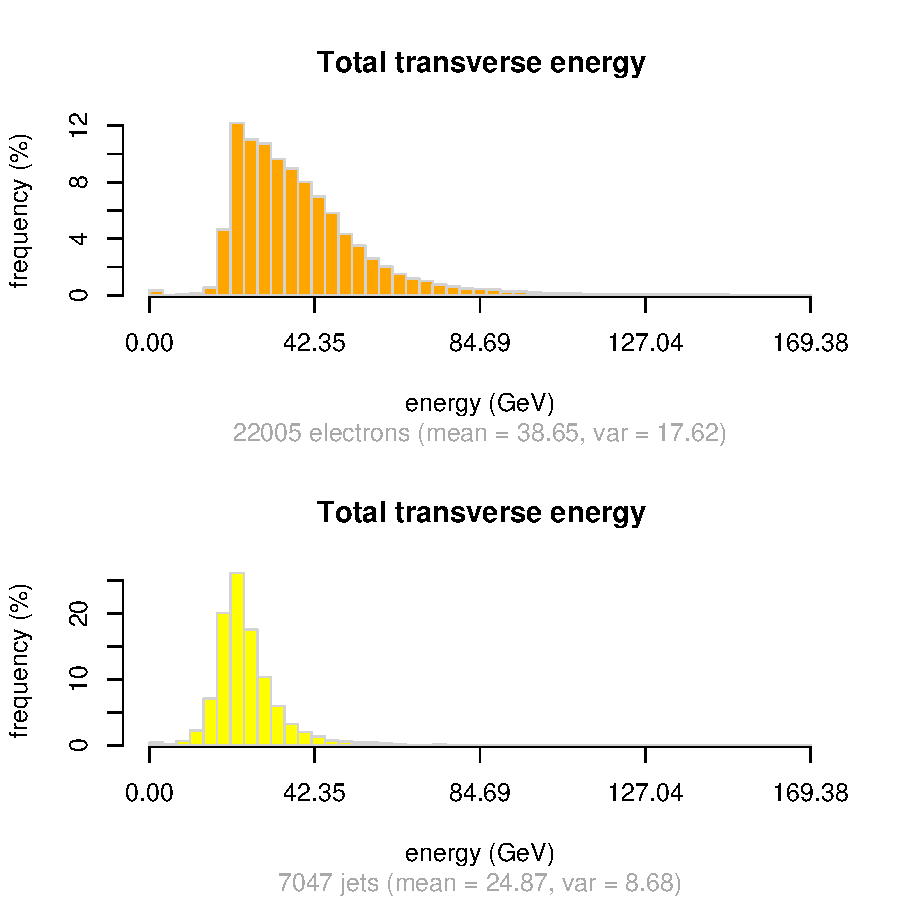
\includegraphics[scale=0.95]{transverse-energy}
\end{center}
\caption{A deposição total de energia em uma região $0,4 \times 0,4$ no plano
$\eta\times\phi$ para elétrons (em cima) e jatos (em baixo) para a massa de
dados disponível para o estudo.}
\label{fig:transverse-energy}
\end{figure}

As Figuras~\ref{fig:em-tenergy} e \ref{fig:had-tenergy} mostram histogramas da
energia transversa total por seção de calorimetria para e\-lé\-trons e
jatos. Nota-se que, para elétrons, quase 100\% da energia total do objeto é
retida na seção e.m., enquanto que, para jatos, observa-se algum vazamento de
energia na seção hadrônica. Embora o corte realizado pelo LVL1 tenha sido em
2~GeV para o vazamento de energia nesta seção, observa-se uma quantidade não
desprezível de eventos com energia hadrônica além deste valor. Por outro lado,
a energia total nesta seção decai rapidamente e assume-se que a existência
desta cauda esteja relacionada à (baixa) qualidade da calibração dos dados
utilizada no LVL1.

\begin{figure}
\begin{center}
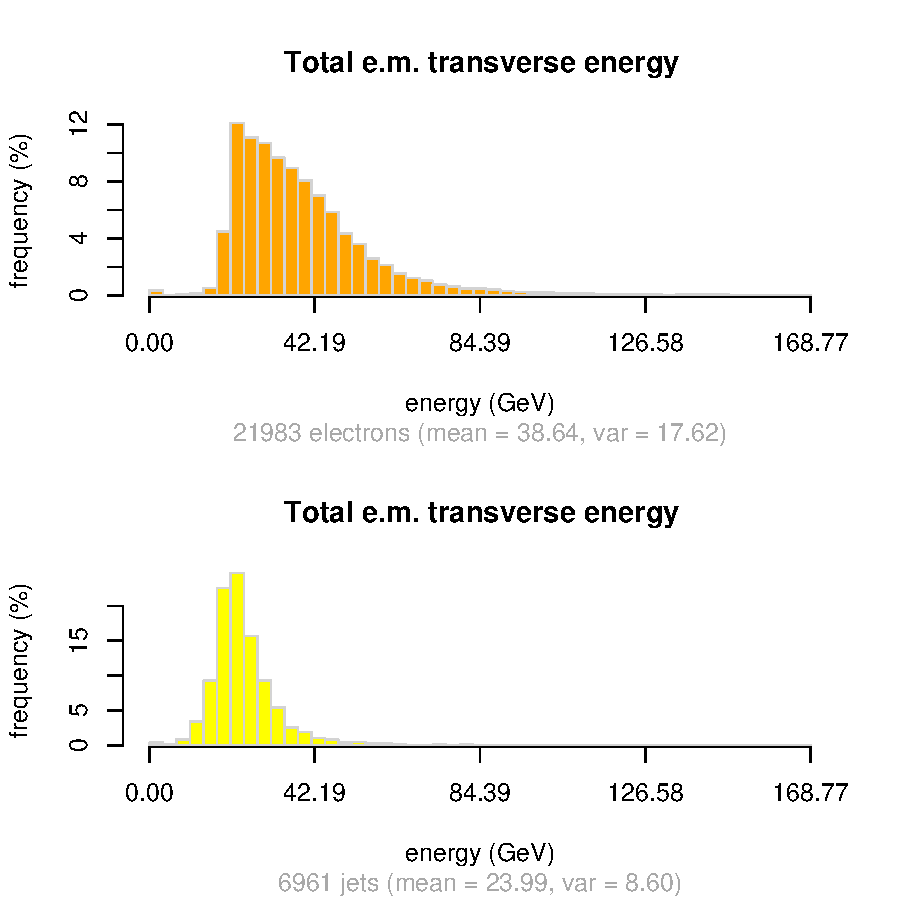
\includegraphics[scale=0.95]{em-tenergy}
\end{center}
\caption{A deposição total de energia na seção e.m. em uma região $0,4 \times
0,4$ no plano $\eta\times\phi$ para elétrons (em cima) e jatos (em baixo) para
a massa de dados disponível para o estudo. As contagens estão normalizadas.}
\label{fig:em-tenergy}
\end{figure}

\begin{figure}
\begin{center}
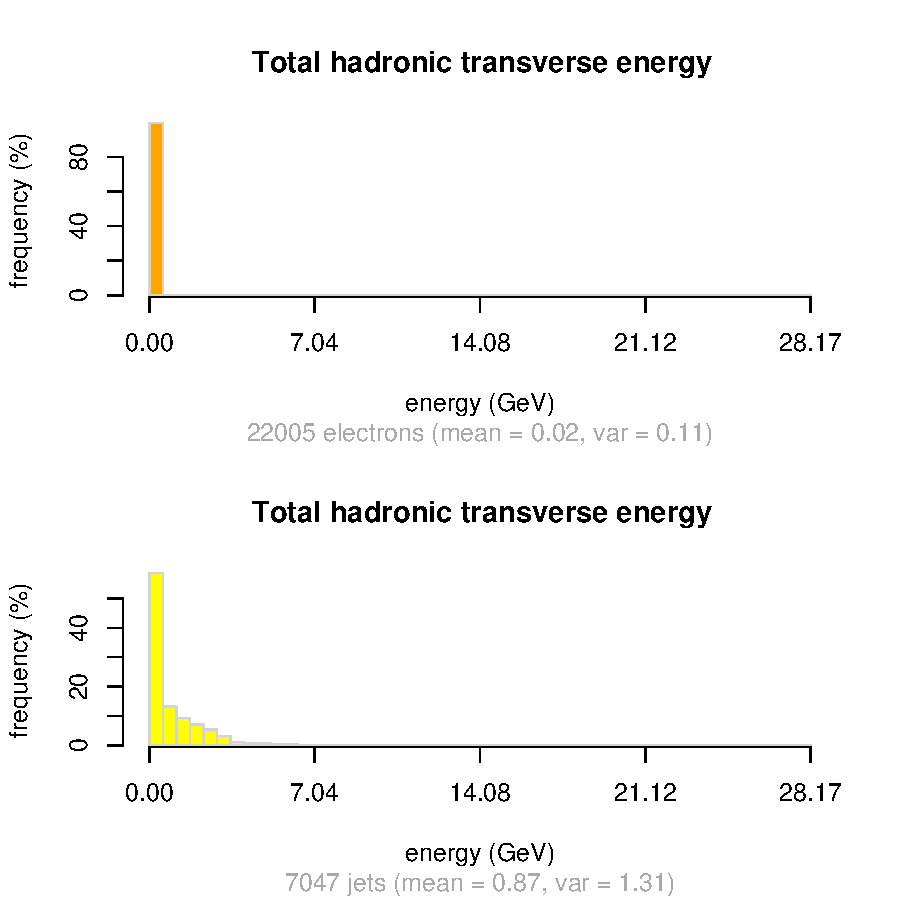
\includegraphics[scale=0.95]{had-tenergy}
\end{center}
\caption{A deposição total de energia na seção hadrônica em uma região $0,4 \times
0,4$ no plano $\eta\times\phi$ para elétrons (em cima) e jatos (em baixo) para
a massa de dados disponível para o estudo. As contagens estão normalizadas.}
\label{fig:had-tenergy}
\end{figure}

As Figuras~\ref{fig:rcore} e \ref{fig:eratio} mostram, respectivamente, a
fração \rcore e \eratio, tal como utilizada pelo EGammaHypo para definir a
eficiência de deteção de elétrons e jatos. Na Figura~\ref{fig:rcore},
observa-se que a distribuição para elétrons tem média bastante próxima a 1 e
baixíssima variância. Para jatos, a média é mais baixa e a distribuição
apresenta longa cauda em direção à origem. No caso da variável \eratio, que
tem por objetivo detetar picos de deposição energética na primeira camada
e.m., para elétrons observa-se um pico dominante em 1, ao passo que, para
jatos, há uma distribuição mais uniforme, indicando uma separabilidade
linear.

\begin{figure}
\begin{center}
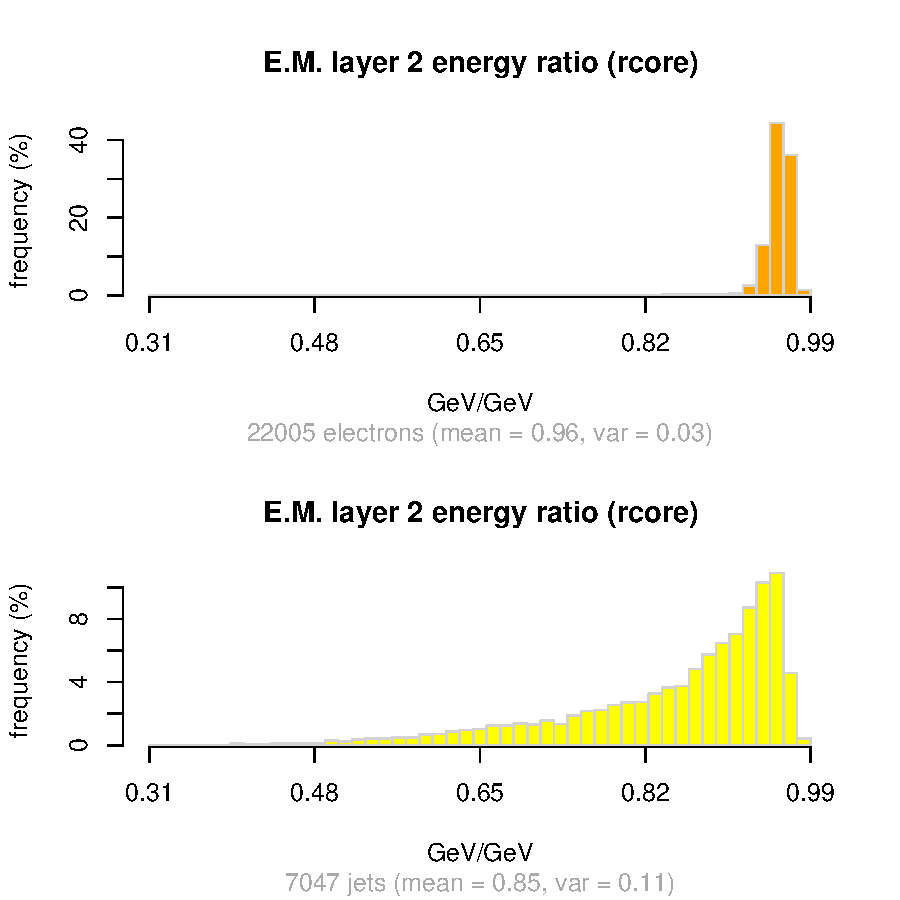
\includegraphics[scale=0.95]{rcore}
\end{center}
\caption{Distribuição da variável \rcore para elétrons (em cima) e jatos
(embaixo). As contagens estão normalizadas.}
\label{fig:rcore}
\end{figure}

\begin{figure}
\begin{center}
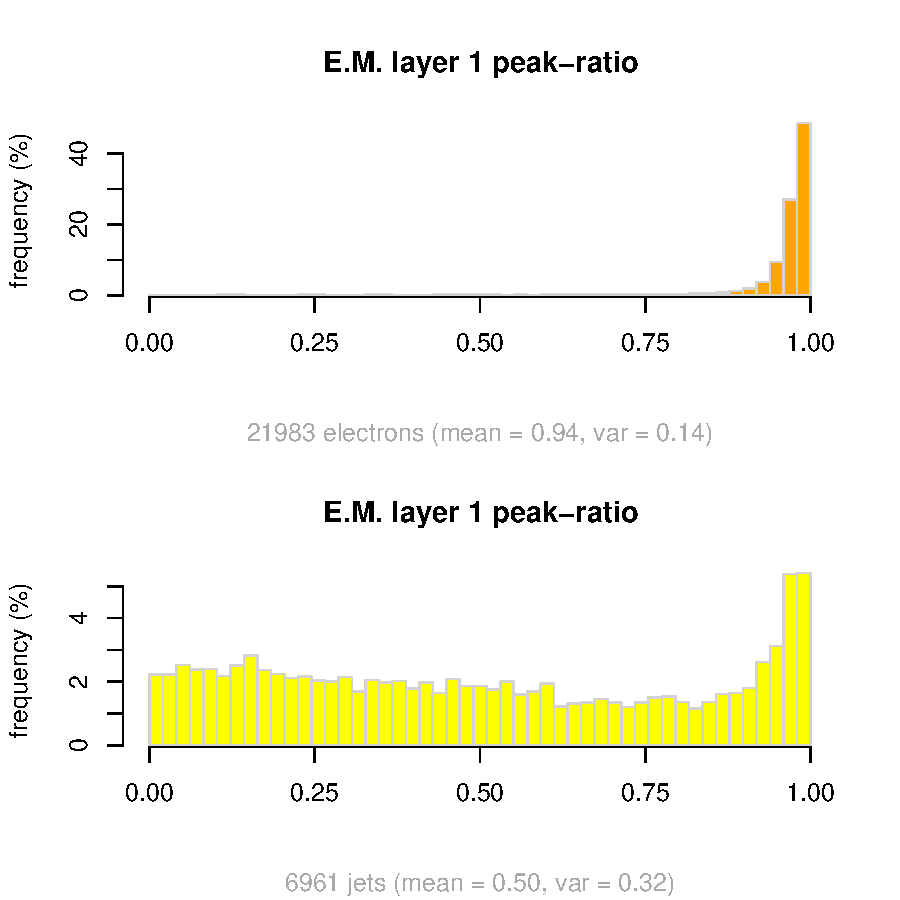
\includegraphics[scale=0.95]{eratio}
\end{center}
\caption{Distribuição da variável \eratio para elétrons (em cima) e jatos
(embaixo). As contagens estão normalizadas.}
\label{fig:eratio}
\end{figure}

As Figuras~\ref{fig:eta} e \ref{fig:phi} mostram histogramas para elétrons e
jatos dos centros refinados pelo T2Calo das RoI's em questão, tanto em relação
à variável $\eta$ quanto à variável $\phi$. É possível distinguir uma
uniformidade na distribuição em $\phi$ e uma tendência a concentração de
eventos nas proximidades de $\eta=0$, como é aguardado no experimento.

\begin{figure}
\begin{center}
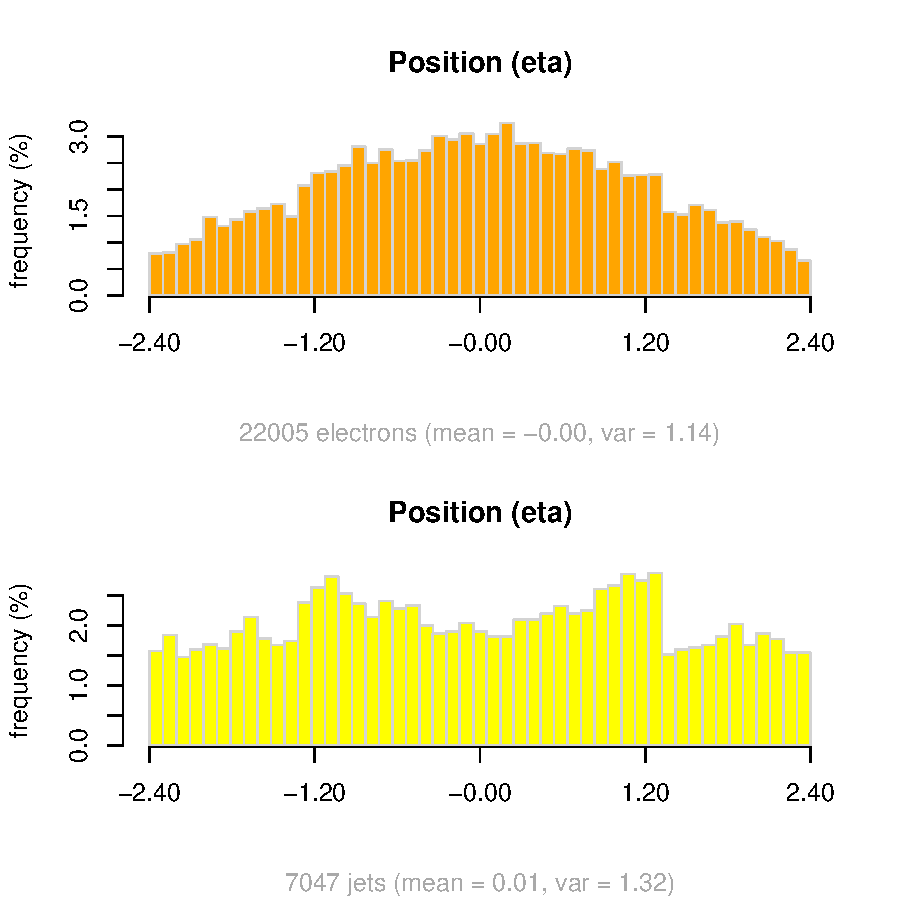
\includegraphics[scale=0.95]{eta}
\end{center}
\caption{Distribuição em $\eta$ dos centros refinados das RoI's para elétrons
(em cima) e jatos (embaixo). As contagens estão normalizadas.}
\label{fig:eta}
\end{figure}

\begin{figure}
\begin{center}
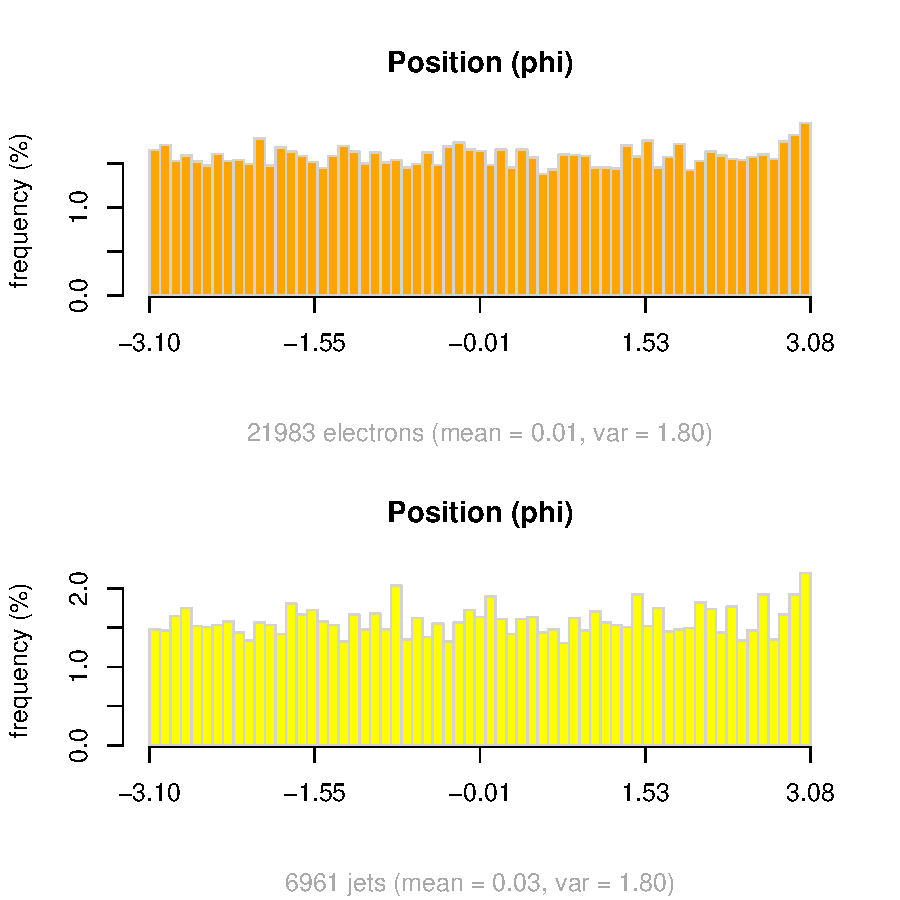
\includegraphics[scale=0.95]{phi}
\end{center}
\caption{Distribuição em $\phi$ dos centros refinados das RoI's para elétrons
(em cima) e jatos (embaixo). As contagens estão normalizadas.}
\label{fig:phi}
\end{figure}

Exceto por eventuais problemas na lógica de simulação (Monte Carlo) e
filtragem (pelo LVL1), estima-se que a massa de dados seja representativa do
problema da separação entre jatos e elétrons. Deve ser levado em consideração
que, para jatos, o pico ao redor de 25~GeV poderá introduzir imprecisões na
definição da capacidade de deteção de elétrons bastante energéticos, presentes
na massa de estudo. Sempre que possível, tentar-se-á levar estas restrições em
consideração.

\subsection{Deteção de elétrons com o EGammaHypo e sua otimização}
\label{sec:eghypo}

Para que a eficiência de deteção do algoritmo proposto pelo EGammaHypo seja
estimada, deve-se passar a massa de dados de estudo por um processo de
otimização que ajude o especialista a selecionar os patamares de corte que
definem o algoritmo, como exposto na Seção~\ref{sec:classic-detection}. Para
tal, dividiu-se o conjunto de dados em 2 metades com aproximadamente o mesmo
número de RoI's. A primeira metade será utilizada para o ``treinamento'' ou
otimização dos cortes, enquanto que a segunda será utilizada para o teste dos
cortes de forma que seja possível testar se, para uma massa de dados jamais
apresentada ao sistema, a eficiência de deteção está de acordo com aquela
encontrada durante a determinação dos cortes. Desta forma, saberemos se o
detetor está demasiado especializado nos dados presentes no conjunto de
treinamento ou pode ser utilizado \emph{genericamente} para a deteção de
elétrons e jatos.

O algoritmo de otimização não será exaustivo, varrendo todo o espaço de dados,
mas partirá de patamares pré-fixados em valores intuitivos e definirá uma
sub-área de variação por onde testará exaustivamente as combinações dos 4
cortes necessários, como é normalmente feito atualmente. Eis aqui os patamares
e passos de busca (ou \emph{possibilidades}) que utilizaremos:

\begin{enumerate}
\item Corte em \rcore: de 0,6 a 1,0, em passos de 0,01 (41 possibilidades);
\item Corte em \eratio: de 0,6 a 1,0, em passos de 0,01 (41 possibilidades);
\item Corte em \etem: de 5000 a 30000 MeV em passos de 500 MeV (51
possibilidades);
\item Corte em \ethad: de 0 a 4000 MeV em passos de 500 MeV (9
possibilidades). 
\end{enumerate}

Para cada corte, a totalidade da massa de dados de treinamento do método é
avaliada e as RoI's que \textit{sobrevivem} ao corte são levadas à próxima
etapa. As eficiências relativas e a quantidade de dados utilizadas para o
teste da fase seguinte são acumulados para posterior análise. Levando-se em
consideração o número de combinações dadas as possibilidades do problema de
otimização e considerando-se que a superfície de erro não possua um único
mínimo, há de se tentar $41 \times 41 \times 51 \times 9 = 771579$ diferentes
combinações, neste caso, antes de qualquer conclusão.

Está claro que uma varredura completa do espaço de parâmetros,
i.e. buscando-se todo o espaço de possibilidades ao invés dos sub-conjunto
utilizados, estaria fora de questão para uma utilização em condições que
possam variar em questão de horas, como é o caso do experimento ATLAS. Desta
forma, seria necessária uma antecipação para os cortes ou uma redução do
espaço de busca, permitindo uma otimização mais rápida. A utilização de
programas especialmente codificados para a tarefa também poderia diminuir o
tempo de teste, tornando o método mais atraente para uma utilização prática.

A Figura~\ref{fig:eghypo-best-sp-train} mostra os resultados da busca
exaustiva definida anteriormente. Esta figura de mérito, normalmente chamada
de \textit{Característica de Operação do Receptor} (do inglês,
\eng{Receiver Operating Characteristics}, ROC \cite{vantrees}), contém os
resultados de cada ponto de operação do algoritmo EGammaHypo. O eixo vertical
denota a eficiência na deteção do sinal de interesse (elétrons), enquanto o
eixo horizontal, a taxa de falso-alarme (erro em jatos) naquele ponto de
operação. A taxa de falso alarme é escalonada em 25~kHz, que é a taxa máxima
de ruído de fundo esperada. O valor do eixo horizontal portanto, denota a
quantidade de jatos que serão aprovados pelo LVL2, como elétrons e, portanto,
representa uma medida direta da taxa de eventos descarregados no Filtro de
Eventos.

Observa-se que, para o conjunto de intervalos testado, a massa de resultados
assume uma forma angular. Ao redor do ponto de flexão, na parte exterior da
massa de resultados, encontraremos as melhores relações de eficiência
\textit{versus} falso-alarme para este discriminador. O ponto destacado nesta
figura representa o conjunto de cortes que maximiza a multiplicação da soma
das eficiências de deteção pelo produto entre elas, ou seja:

\begin{equation}
SP = (\text{efic.}_{classe_1} + \text{efic.}_{classe_2}) \times
(\text{efic.}_{classe_1} \times \text{efic.}_{classe_2})
\label{eq:sp-product}
\end{equation}

O produto SP de um detetor para 2 classes de eventos apresenta um máximo
($=2,0$) quando a eficiência na deteção de ambas as classes é máximo
(i.e. $=1,0$), e um mínimo em $0$ quando a eficiência de deteção de
\textbf{qualquer} uma das duas classes de eventos é $0$. É interessante notar
que, para um determinado classificador, o valor do máximo da
Equação~\ref{eq:sp-product} indicará o ponto de inflexão da curva R.O.C.. Este
ponto determina a melhor relação de deteção entre as duas classes de eventos
para o classificador.

À medida que a curva R.O.C. se aproxima, em detrimento de uma melhora na
eficiência de deteção, do eixo vertical para $\text{Prob.}_\text{falso-alarme}
= 0$ e do eixo horizontal para $\text{Prob.}_\text{deteção} = 1,0$, o máximo
da Equação~\ref{eq:sp-product} aumentará. Por esta razão utilizar-se-á o valor
máximo produto SP de um detetor como uma figura de mérito de sua eficiência de
classificação.

No caso específico em análise, o ponto onde produto SP atinge seu máximo
determina uma eficiência de deteção de elétrons de 91,85\% contra 10,19\% de
falso alarme na deteção de jatos, ou 2,55 kHz, levando-se em consideração a
contaminação do canal de elétrons na saída do LVL1. O valor do produto SP no
ponto em questão é de $1,50$.

\begin{figure}
\begin{center}
\includegraphics[scale=0.98]{eghypo/eghypo-best-sp-train}
\end{center}
\caption{A curva ROC para 771.579 combinações de valores de corte para o
algoritmo EGammaHypo.}
\label{fig:eghypo-best-sp-train}
\end{figure}

Os seguintes valores de corte determinam o detetor marcado na
Figura~\ref{fig:eghypo-best-sp-train}:
\begin{enumerate}
\item \rcore: 0,93;
\item \eratio: 0,82;
\item \etem: 14.500 MeV;
\item \ethad: 500 MeV.
\end{enumerate}

Aplicando-se estes cortes ao conjunto de teste, de forma análoga, obtém-se
91,62 \% de eficiência na deteção de elétrons contra 10,45 \% de falso-alarme
($SP = 1,49$). Este resultado indica também que os dois sub-conjuntos de dados
(treino e teste) são estatisticamente semelhantes. Durante a busca exaustiva
deste resultado, acumularam-se os resultados de eficiência e falso-alarme
parciais entre operações de corte. Estes valores podem ser vistos na
Tabela~\ref{tab:eghypo-partials}. Como é possível avaliar, a partir desta
tabela, as variáveis \rcore e \eratio são as mais discriminatórias, deixando
passar apenas cerca de 30 \% e 45 \% dos jatos avaliados, respectivamente. O
corte em \etem não reduz a taxa de eventos, sendo praticamente irrelevante a
este processo de discriminação. Este comportamento é esperado, para a massa de
dados sendo avaliada, uma vez que os jatos disponíveis tem energia fixa em 25
GeV e que elétrons estão espalhados no espectro de energia. O vazamento de
energia na seção hadrônica (último corte), ainda conseguirá diminuir a taxa de
falso-alarme na saída do detetor.

%% COMENTÁRIO: SERIA BOM DIZER PORQUE O CORTE EM EM_ET NÃO É TÃO RELEVANTE...
%% IDÉIAS: ALTA CORRELAÇÃO COM RCORE E ERATIO => PCA?

\begin{table}
\caption{Valores parciais de deteção e falso-alarme para o detetor baseado no
algoritmo EGammaHypo.}
\label{tab:eghypo-partials}
\begin{center}
\begin{tabular}{|l|l|r|r|}
\hline
\textbf{Ordem} & \textbf{Variável} & \textbf{Eficiência (\%)} &
\textbf{Falso-alarme (\%)} \\ \hline
1 & \rcore & 96,4 & 30,5 \\ \hline
2 & \eratio & 95,7 & 43,6 \\ \hline
3 & \etem & 99,9 & \textbf{98,9} \\ \hline
4 & \ethad & 91.8 & 77.4 \\ \hline
\end{tabular}
\end{center}
\end{table}

As Figuras~\ref{fig:eghypo-eta-scan-test}, \ref{fig:eghypo-phi-scan-test} e
\ref{fig:eghypo-emet-scan-test} mostram os valores parciais de eficiência e
falso-alarme considerando-se uma divisão dos dados por $\eta$, $\phi$ e por
energia total transversa na seção e.m. dos calorímetros. No caso da varredura
em $\eta$, é possível notar que a eficiência de deteção do método apresenta
uma queda abrupta próximo ao vão entre a seção do barril e da tampa ($\eta
\approx 1,5$), o que é esperado devido a ausência de elementos de deteção
nesta área. Para a varredura em $\phi$, observa-se uma distribuição bastante
homogênea para a eficiência de deteção de elétrons e jatos, apesar da baixa
estatística para jatos em alguns intervalos em $\phi$ (muitos canais possuem
apenas 30 a 40 jatos, como é possível observar na
Figura~\ref{fig:transverse-energy}). A varredura por \etem indica que o método
é bastante robusto na deteção de elétrons, aumentando sua eficiência
suavemente com o valor de energia da RoI. Este comportamento é esperado pois
sabe-se que a resolução em energia de um calorímetro aumenta com a energia do
objeto \cite{wigmans-book} e, portanto, a capacidade discriminante do
sistema. Por outro lado, jatos mais energéticos tendem a penetrar ainda mais
no calorímetro, fazendo com que a deteção de elétrons se torne mais fácil. O
falso-alarme em jatos também aumenta com a energia do objeto analisado, embora
seja difícil estimar com precisão a qualidade do valor de falso-alarme
determinado, uma vez que a estatística para jatos acima de 50 GeV é
praticamente inexistente.

\begin{figure}
\begin{center}
%\includegraphics[angle=90,width=15cm,height=20cm]{eghypo-eta-scan-test}
\includegraphics[scale=0.98]{eghypo/eghypo-eta-scan-test}
\end{center}
\caption{Eficiência de deteção contra falso-alarme por $\eta$ para o conjunto
de testes utilizando o algoritmo EGammaHypo.}
\label{fig:eghypo-eta-scan-test}
\end{figure}

\begin{figure}
\begin{center}
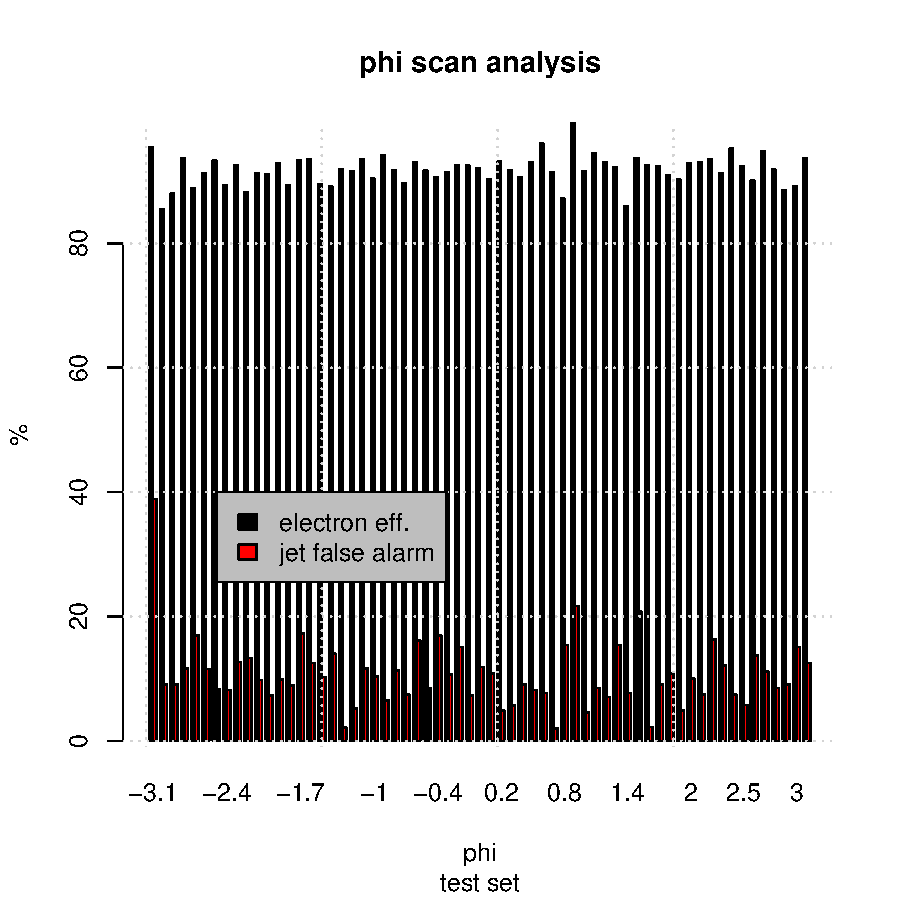
\includegraphics[scale=0.98]{eghypo/eghypo-phi-scan-test}
\end{center}
\caption{Eficiência de deteção contra falso-alarme por $\phi$ para o conjunto
de testes utilizando o algoritmo EGammaHypo.} 
\label{fig:eghypo-phi-scan-test}
\end{figure}

\begin{figure}
\begin{center}
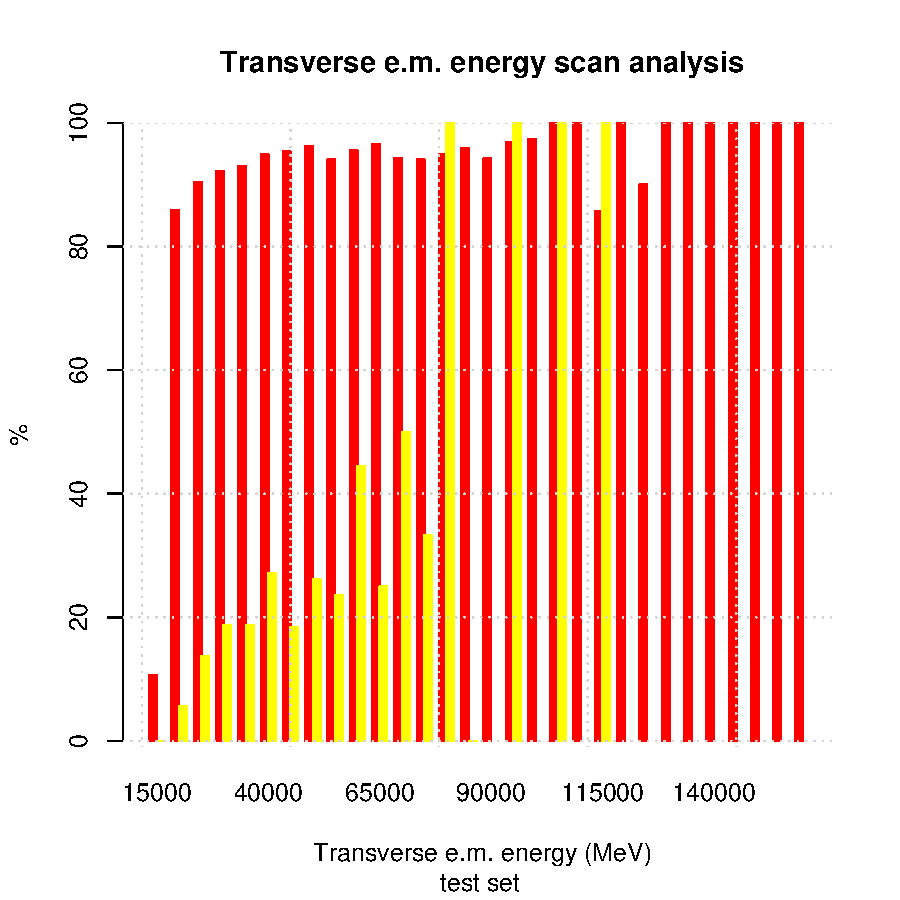
\includegraphics[scale=0.98]{eghypo/eghypo-emet-scan-test}
\end{center}
\caption{Eficiência de deteção contra falso-alarme por \etem para o conjunto
de testes utilizando o algoritmo EGammaHypo.}
\label{fig:eghypo-emet-scan-test}
\end{figure}

%\subsection{Análise de Componentes Principais}

%Isto não é óbvio que melhorará a análise do método já que temos poucas
%variáveis a a informação contida nelas traz bastante informação, mas não
%informação discriminante.

%Levando-se em consideração os dados da Tabela~\ref{tab:eghypo-partials}, é
%possível intuir que exista uma grande correlação entre as 4 variáveis
%definidas pelo T2Calo e utilizados pelo EGammaHypo para a deteção de
%elétrons. A técnica de Análise de Componentes Principais \cite{vantrees}
%define uma transformação linear que, quando aplicada a massa de dados de onde
%é originalmente extraída, completamente a descorrelaciona. Esta transformada
%é comumente conhecida como KLT (do inglês \eng{Karhunen-Loève Transform}).

%Uma das técnicas para o cálculo da KLT utiliza a matriz de covariância C do
%conjunto de dados de analisados para calcular 

%\cite{vantrees}, é possível calcular a transformação , que
%completamente descorrelacionará os dados disponíveis. 

\typeout{ *************** End of file baseline.tex *************** }

%% Hello emacs, this is -*- latex -*-
\typeout{ ====================================================================}
\typeout{ This is file neural.tex, created at 27-Aug-2005 }
\typeout{ Maintained by Andre Anjos <Andre.dos.Anjos@cern.ch> }
\typeout{ ====================================================================}

\chapter{Sistema neural de deteção elétron/jato baseado em calorimetria}
\label{chap:neural}

Neste capítulo, define-se um sistema de extração de característica em anéis de
deposição energética, associado a um sistema de discriminação neural, para o
projeto de um classificador de partículas ótimo para o Segundo Nível de
Filtragem do experimento ATLAS. Este classificador supera significativamente
em desempenho o sistema clássico de deteção que é usado como base no
experimento ATLAS. O sistema proposto tem ainda as vantagens de ser modular,
rápido e de simples manutenção.

\section{Revisão da literatura}
\label{sec:review}

%\textit{Introduzir um histórico de das diversas técnicas até hoje, emprego de
%RN em HEP, Hera, D0, LEP. Faltando...}

%Perfil:

%\begin{itemize}
%\item Entre 10-15 páginas máximo;
%\item[OK] Bruce Demby escreveu um review completo na NIM;
%\item[OK] Chrss Kiesling implementou RN no Trigger do H1, autor do processo de
%relevância? 
%\item Verificar publicações no CERN, Fermilab e Desy (\eng{via} SPIRES?);
%\item Verificar publicações nos congressos (IEEE, ACAT, ISCAS, de 2000 para
%cá); 
%\item[OK] Redes Neurais e mapeamento topológico em calorimetria (Wisconsin);
%\item Por alto como se fazia no LEP;
%\item \textbf{Seixas}: coloque aqui outras idéias...
%\end{itemize}

Os primeiros sistemas de deteção baseados em redes neurais artificiais,
aplicados à Física de altas energias, surgiram em 1987, na reconstrução de
partículas carregadas e píons neutros \cite{denby-nim-1997}. Hoje em dia
\cite{denby-nim-2004}, cerca de 20 anos passados, tais sistemas são empregados
em praticamente todas as áreas neste campo, desde da concepção de detetores
\cite{wilk-nim-2006}, filtragem e aquisição de dados
\cite{denby-nim-2003, kohne-nim-1997, varela-cms-1998},
passando pela reconstrução \eng{offline} \cite{peterson-nim-1988} e análise
\cite{kiesling-nim-2004}. Nestes ambientes, o reconhecimento de padrões pode
ocorrer tanto num plano mais elementar, onde deseja-se identificar os
parâmetros de cada partícula que surge de uma reação sub-atômica, quanto num
plano mais avançado, onde combina-se as informações detetadas para se tentar
definir as características globais de um evento.

\subsection{Redes neurais para análise e reconstrução \eng{offline}}

\subsection{Reconstrução de agrupamentos em calorímetros}

\subsection{Redes neurais em sistemas de filtragem}

A taxa de falsos-positivos em um experimento em física de altas energias pode
ser bastante grande, chegando muitas vezes a ser ordens de magnitude mais
elevadas que o sinal que se deseja detetar. Somado a este fator, incluem-se as
restrições de tempo de processamento de um sistema de filtragem que deva
operar em tempo real, processando, milhões de eventos por segundo.

O primeiro sistema de filtragem baseado em redes neurais foi construído e
testado em 1992, no Fermilab, Estados-Unidos, para o experimento $D0$ no
Tevatron \cite{lindsey-nim-1992}. Este sistema pode determinar os parâmetros
da trajetória de múons levando em consideração valores de tensão digitalmente
amostrados de uma câmara dividida em três planos, cada um contendo várias
células de deteção. Cada célula é equipada com placas coletoras de tensão que
permitem a amostragem da distância relativa da partícula com relação aos
dipolos através do atraso do sinal de avalanche disparado pela interação do
múon com a célula de deteção.

Levando-se em consideração os valores de atraso em cada célula e que a
partícula atravessará todas as camadas do detetor, é possível calcular o ponto
de impacto aproximado e ângulo da trajetória da partícula. Para tal, uma
rede neural tipo MLP com 64 neurônios escondidos e 64 saídas, baseada em
\eng{hardware} especializado (chip Intel ETANN), é treinada levando-se em
consideração os sinais de interação de cerca de 10.000 múons com este
detetor. Estes eventos foram simulados através de processos de Monte-Carlo. O
treinamento em si ocorre em um PC que emula o sistema em \eng{hardware}. Os
pesos podem então ser descarregados no processador e utilizados
\eng{online}.

Os resultados encontrados por este sistema são surpreendentemente positivos em
comparação com métodos de reconstrução \eng{offline}. Considerando-se um
conjunto de testes de alguns milhares de traços, o sistema baseado no
processador neural obtém um erro menor que 5 mm no ponto de impacto na
primeira camada de 96\% (contra 98\% de um sistema de \eng{fitting}
\eng{offline}). Para o coeficiente angular, este sistema possui um erro menor
que $5,7^{o}$ para 93\% (contra 97\% \eng{offline}) para os padrões de
teste. O tempo total de processamento do sistema é de apenas 8~$\mu$s.

O experimento H1, que utiliza o acelerador HERA no laboratório Desy em
Hamburgo, Alemanha, estuda a distribuição do momento dos constituentes de
prótons e mede a força de acoplamento do glúon aos diferentes quarks. Devido à
interações tais como as que ocorrem entre o feixe e resíduos no tubo do
acelerador, a taxa de eventos que constituem ruído de fundo chega a uma ordem
de $10^5$ comparada à ocorrência de física interessante. Para filtrar a taxa
de eventos inicial de cerca 10 milhões por segundo para apenas 100, este
experimento utiliza um sistema de filtragem divido em 4 níveis. O primeiro
nível de filtragem reduz a taxa de eventos em cerca de 100 vezes. Desta forma,
o segundo nível de filtragem tem apenas cerca de 10~$\mu$s para tomar uma
decisão. Este nível deve reduzir a taxa de eventos aproximadamente 10
vezes. Uma rede neural foi utilizada para resolver este problema
\cite{kohne-nim-1997}. 

No primeiro nível de filtragem, 16 variáveis são calculadas tais como a
energia total, transversal e na parte centrais do calorímetro, dentre
outras. Este nível de filtragem ignora, no entanto, quaisquer relações entre
estas variáveis. Cortes mais sofisticados podem ser executados no segundo
nível adicionado-se à estas variáveis, outras quantidades que somente estão
disponíveis após o tempo de decisão do primeiro nível e alimentando-se uma
rede neural tipo MLP. 

As variáveis selecionadas (somas de energias, número de partículas com carga
detetadas, etc.) são utilisadas para determinar se o evento em questão advem
de uma interação elétron-próton (física de interessante), de uma interação do
feixe com uma molécula no tubo do acelerador ou qualquer outro fenômeno a ser
desprezado. O sistema é implementado em \eng{hardware}, utilizando o
processador CNAPS 1064, da empresa Adaptive Solutions, executando em um tempo
total de 20~$\mu$s. Cada canal de decaimento é estudado separadamente e uma
rede especialista utilizada para detetar sua ocorrência.

A eficiência do sistema é variável conforme o canal em análise e apresentada
neste trabalho levando-se em consideração a taxa de redução de eventos
representando falso-alarme com relação ao primeiro nível de filtragem. Esta
taxa chega a valores entre 40 e 160 para eventos tipo $\gamma p \rightarrow X
+ J/\Psi$ e de 10 a 20 para eventos tipo $\gamma p \rightarrow \text{jatos}$,
o que está acima das especificações originais para o sistema de
filtragem. Nestes casos, o sistema neural permitiu que se elimine
complementamente pré-escalonamento no primeiro nível, aumentando
substancialmente o número de eventos interessantes registrados em mídia
permanente.

\subsection{Redes neurais e calorimetria em sistemas de filtragem}

Em \cite{varela-cms-1998}, descreve-se um sistema de deteção neural de
elétrons em tempo real que utiliza-se das informações dos calorímetros e.m. do
experimento CMS \cite{cms-trigger}. O primeiro nível de filtragem desta
experiência não exaure a informação provida pelo calorímetro e.m. e portanto
há oportunidade para que um segundo nível de filtragem, apoiando-se na
informação não aproveitada pelo LVL1, consiga atingir alguma redução na taxa
de eventos que será repassado ao terceiro nível de filtragem.

A informação utilizada para a deteção de elétrons são os valores de energia de
um conjunto de células provenientes dos cristais do calorímetro e.m.. Este
conjunto define um ``quadrado'' de aproximadamente 7 por 7 células deste
detetor, cobrindo uma área de aproximadamente $0,1 \times 0,1$ no plano $\eta
\times \phi$. O algoritmo escolhido inicia o processamento localizando o pico
de deposição energética na região. Em seguida, de forma a tornar o processo de
deteção independente da energia, normaliza-se o valor de deposição energética
em cada célula pelo valor de energia na célula mais energética. Para
amplificar os valores de deposição energética nas bordas da região em análise,
tira-se a raíz quadrada do valor normalizado das células.

Cada região analisada, composta de 49 valores de energia normalizada, é
disponibilizada como entrada a uma rede neural tipo MLP, com 8 neurônios
escondidos, treinada para detetar jatos e elétrons. A base de dados inicial
consistia de 50.000 jatos e 15.000 elétrons simulados com energia entre 5 e
225 GeV. Estes eventos são submetidos a uma filtragem por um sistema de
simulação do LVL1 do CMS, definindo-se a base de dados disponível para
treinamento: 1.500 jatos e por volta de 13.000 elétrons. Para uma taxa
constante de deteção de elétrons de 98\%, obteve-se uma taxa de deteção de
jatos de 71\% para eventos com ruído de fundo equivalente a um ambiente
simulado de alta luminosidade ($10^{34}\text{cm}^{-2}\text{s}^{-1}$) e 78\%,
para um ambiente em baixa luminosidade ($10^{33}\text{cm}^{-2}\text{s}^{-1}$).

\subsection{Tendências}

%Palavras-chave: pré-processamento, baixa latência, encapsulamento de ruído,
%determinação de parâmetros, MLP

%Describe stuff for ATLAS, like \cite{daq11}, \cite{daqnote00-02} and
%\cite{abramowicz-nim-2004}. 

\section{Discriminação linear}
\label{sec:lms}

O discriminador de Fisher \cite{fisher} ou a Análise de Discriminação Linear
descrevem algoritmos bem definidos para que se maximize a capacidade
discriminante de um corte no plano com N dimensões, que separa duas classes de
amostras \cite{duda}. Esta técnica requer que determinadas características nas
amostras estejam presentes, entre elas, que os dados apresentem uma
distribuição gaussiana e que as matrizes de covariância para ambas as classes
em separado sejam idênticas\footnote{A Análise de Discriminação Quadrática, no
entanto, demonstra que esta característica pode ser relaxada considerando-se
que seja sempre possível projetar, através de uma transformação linear, o
espaço de entrada em um outro espaço onde as matrizes de covariância sejam
iguais e portanto recaindo no caso simples.}. Muitas vezes, na prática, os
valores de média e a covariância não estão disponíveis e devem ser estimados,
o que normalmente leva a falhas no cálculo do ponto ótimo de
discriminação. Dentre as técnicas de estimação da média e covariância, pode-se
destacar a estimação por máxima verossimilhança ou por máximo a
\textit{posteriori} \cite{duda}.

De posse dos valores de média e covariância das classes, o plano de separação
seria definido da seguinte forma:

\begin{equation}
\overrightarrow{w} = \Sigma^{-1}(\overrightarrow{\mu}_0 -
\overrightarrow{\mu}_1) 
\label{eq:weight-1}
\end{equation}

O operador $\Sigma$ na Equação~(\ref{eq:weight-1}) representa a covariância ou
\textit{variância cruzada} das observações do universo de entrada e $\mu$ as
médias das duas classes de eventos que se deseja separar. Um problema que se
segue é da inversibilidade de $\Sigma$, que dependerá de quão bem o conjunto
de amostras representa as classes a serem discriminadas. Por exemplo, se
$\Sigma$ possui combinações lineares dos dados disponíveis, o ranque desta
matriz será inferior ao número de amostras e portanto a matriz não será
inversível. Embora existam maneiras de superar o problema, é possível fazer
uso de outras técnicas derivadas deste sistema primário para que se maximize a
discriminação das classes de eventos dado um conjunto de amostras.

Por causa das dificuldades discutidas, muitas técnicas iterativas surgiram
para que seja possível a definição de um plano ótimo de separação linear à
partir de amostras de dados reais. Dentre elas, o algoritmo do Mínimo Médio
Quadrático \cite{widrow} (do inglês \eng{Least Mean Square} ou LMS) é um dos
mais utilizados. Este método pode ser considerado um caso especial de uma rede
neural totalmente conectada e sem realimentação (veja Seção~\ref{sec:neural}
para uma discussão mais detalhada), com as seguintes ressalvas:

\begin{itemize}
\item Há somente um neurônio conectando todas as entradas com a saída da rede;
\item A função de ativação deste neurônio ($\phi(\dot)$) é a função identidade
$f(x) = x$.
\end{itemize}

Para o treinamento, definem-se alvos para as duas classes de eventos e a
função de erro:

\begin{equation}
E(\overrightarrow{w}) = \frac{1}{2} e^2(n)
\label{eq:mse-definition}
\end{equation}

Nesta equação, $\overrightarrow{w}$ é o vetor de pesos que define o plano de
separação linear e $e(n)$ é o erro na saída da rede com relação ao alvo para a
classe escolhida na amostra $n$, ou seja $e(n) = d(n)-y(n)$ ($d(n)$ é o
alvo). Desta forma, derivando-se esta função de erro com relação aos pesos
sinápticos $\overrightarrow{w}$, mostra-se que o gradiente de $E$ será:

\begin{equation}
\frac{\partial E(\overrightarrow{w})}{\partial \overrightarrow{w}} =
-x(n)e(n) 
\end{equation}

Nesta equação, $x(n)$ representa a n-ésima entrada que leva o neurônio linear
a uma saída $y(n)$. E, com este resultado, define-se a fórmula de treinamento
do LMS:

\begin{equation}
\hat{w}(n+1) = \hat{w}(n) + \alpha x(n)e(n)
\label{eq:lms}
\end{equation}

Nesta equação, $\alpha$ representa a taxa de aprendizagem, um parâmetro para a
suavização da trajetória do treinamento no espaço da função de erro
$E(\overrightarrow{w})$. A Equação~(\ref{eq:lms}) representa a fórmula
clássica do treinamento de um classificador LMS, indicando um método
bem-definido de atualização dos pesos da rede para que se convirja a um erro
mínimo. Em implementações realísticas de um classificador LMS, é possível
agrupar a correção dos pesos $\hat{w}$ em bateladas ou épocas de forma que se
suavize a migração do sistema para o mínimo global. No treinamento em épocas,
os pesos sinápticos são corrigidos tendo por base a média dos erros para todos
os eventos de uma época, ao invés da atualização instantânea proposta pela
Equação~(\ref{eq:lms}).

Como é possível inspecionar diretamente na Equação~(\ref{eq:lms}), os pesos do
detetor são atualizados segundo um produto interno dos erros multiplicados
pelas respectivas entradas, uma época do treinamento. No caso de existirem
grandes diferenças de magnitude entre as variáveis de entrada de um sistema
LMS, é possível que o processo de treinamento se torne tendencioso em função
destas variáveis. Para eliminar o risco de tendência no treinamento devido a
magnitude das componentes da entrada, é também prática que cada entrada seja
subtraída da sua média e dividida pela sua variância.

Finalmente, a Figura~\ref{fig:lms-flow} mostra o diagrama de blocos do
discriminador LMS que será empregado neste estudo. O valor da saída $y$ é
utilizado para definir a R.O.C. do discriminador e escolher, ao invés de
quatro, apenas um corte que maximize a capacidade discriminante do
sistema. Alvos ($t$) para cada uma das classes são escolhidos e o sinal de
erro é utilizado para corrigir os pesos sinápticos, até que o sistema convirja
para o erro mínimo.

\begin{figure}
\begin{center}
\includegraphics{lms-flow}
\end{center}
\caption{O diagrama de fluxo do discriminador LMS que será empregado na
discriminação elétron-jato.}
\label{fig:lms-flow}
\end{figure}

\subsection{Implementação do LMS na separação e\-lé\-tron-jato}
\label{sec:lms-ej}

Levando-se em consideração as 4 variáveis definidas pelo T2Calo, é possível
encontrar o plano quadri-dimensional que define um discriminador linear ótimo,
usando-se o algoritmo LMS, como descrito anteriormente. A separação em classes
de treinamento e teste, como apresentada na Seção~\ref{sec:eghypo}, será
re-aproveitada aqui, para que seja possível a comparação dos resultados nos
dois casos.

O sistema de treinamento e teste foi implementado em um ambiente de trabalho
C++, seguindo o paradigma da orientação à objetos (OO) \cite{stroustrup,
booch}. Este ambiente, que será re-utilizado em várias partes deste trabalho,
será discutido em detalhes na Seção~\ref{sec:framework}. A
Figura~\ref{fig:train-flow} contém um diagrama de fluxo com os diversos passos
do sistema de treinamento implementando. Inicialmente, os bancos de dados
usados para o treinamento e teste da rede são carregados. Os valores de média
e variância dos dados, levando-se em consideração a estatística de cada uma
das classes de dados, são extraídos do conjunto de treinamento e guardados
juntos aos pesos $\hat{w}(n)$, para que sejam aplicados durante o
treinamento\footnote{De fato, seria mais eficiente que os fatores de
normalização fossem aplicados previamente ao treinamento. No entanto, uma vez
que deseja-se re-aproveitar a base de código para rodar o discriminador em uma
etapa seguinte, é mais simples do ponto de vista da implementação que a
normalização seja aplicada como parte do passo de execução do
discriminador.}. Os pesos sinápticos são aleatoriamente inicializados (entre
$-1$ e $+1$). Valores-alvo para cada uma das classes são pré-fixados: $-1$
para elétrons e $+1$ para jatos. O processo de treinamento é então
disparado. Para cada época ou batelada de treinamento, um conjunto de elétrons
e jatos é escolhido aleatoriamente à partir dos bancos-de-dados
disponíveis. Os valores de erro são calculados e sua média é aplicada para a
correção dos pesos sinápticos, considerando a taxa de aprendizagem
$\alpha$. As melhores redes, tomando-se o valor do produto SP como referência,
são guardadas a cada passo de treinamento. 

\begin{figure}
\begin{center}
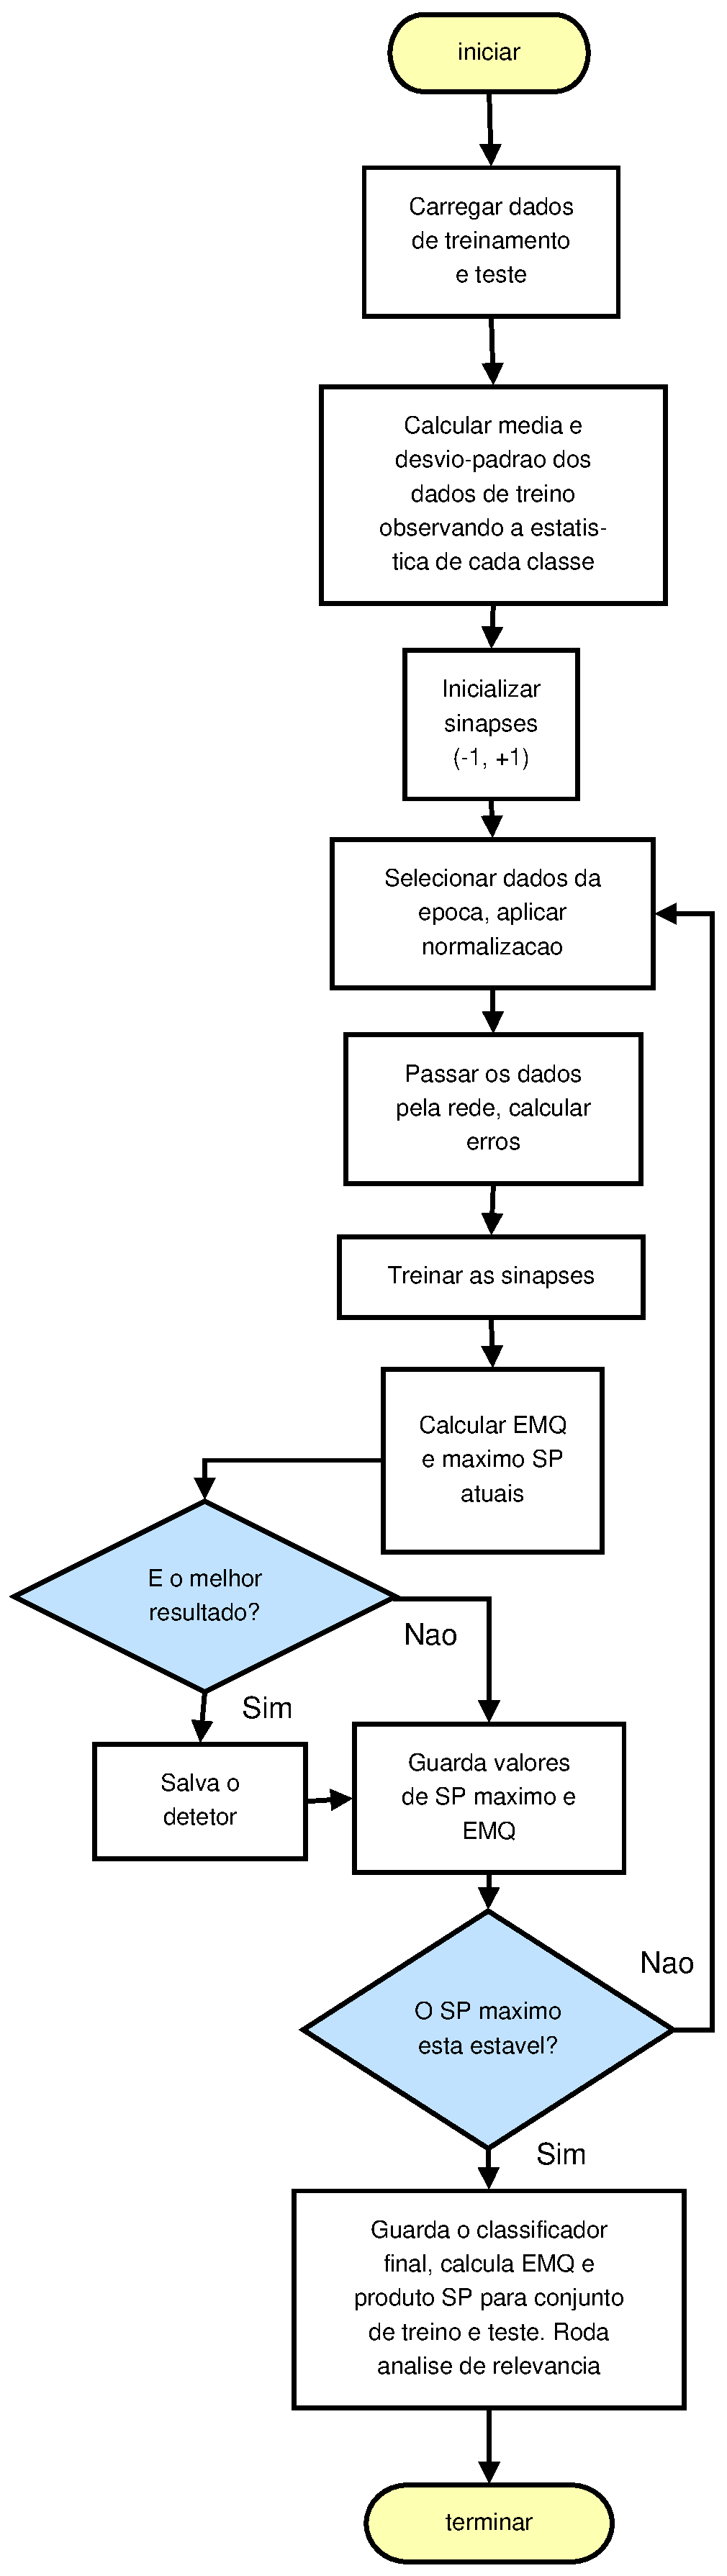
\includegraphics[scale=0.35]{train-flow}
\end{center}
\caption{O fluxo implementado para o treinamento do discriminador LMS.}
\label{fig:train-flow}
\end{figure}

Um sistema configurável é utilizado para detetar a estagnação do
treinamento. Este sistema baseia-se na observação do valor do produto SP para
o conjunto de teste. Quando este valor atinge um estado no qual as alterações
sinápticas não o modificam significativamente (levando-se em consideração uma
margem de erro configurável), e por um número de iterações, o treinamento é
automaticamente parado. O melhor discriminador até então é recarregado. Um
estudo dos valores de Erro Médio Quadrático (EMQ, do inglês \eng{Mean-square
error}, MSE) é feito para os conjuntos de treinamento e teste. O produto SP
máximo também é avaliado para os dois conjuntos de dados. Esta técnica tem o
objetivo de evitar um treinamento excessivo da rede (do inglês
\eng{overtraining}) fazendo com que ela se especialize em demasiado nestes
dados sem conseguir ter uma capacidade de discriminação generalizada. O valor
da variação do produto SP a partir do qual considera-se que o sistema esteja
estagnado dependerá do problema. Valores típicos estão na ordem de $10^{-3}$.

Para este trabalho, optou-se pela a não utilização de um conjunto de validação
do sistema de deteção. Este conjunto poderia ser utilizado para verificar a
operação do sistema após o treinamento. No entanto, a física disponível para o
estudo é limitada devido a natureza de geração de eventos. Para se realizar
uma análise baseada no LVL2, elétrons e jatos que passem a um corte do LVL1
devem ser simulados, uma vez que o LHC ainda não encontra-se operacional. 

A taxa de redução do LVL1 é bastante expressiva, atingindo uma redução de
aproximadamente 1000 vezes na taxa de contaminação de elétrons. Desta forma,
para produzir 1000 jatos que passariam a um corte do LVL1 é necessário que se
produza cerca de 1 milhão de eventos deste tipo. Cada simulação de um evento
pode durar muitos minutos, às vezes horas de processamento do poder de
computação disponível.

%Por outro lado, a física simulada é representativa do tipo de partículas
%que deseja-se analisar.

\subsection{Resultados da aplicação do LMS na separação e\-lé\-tron-jato}

Utilizando o sistema descrito anteriormente e a separação dos dados (em
classes de treinamento e teste) proposta no início do estudo, realizou-se um
conjunto de testes para a determinação de um discriminador linear ótimo
baseado nas quatro variáveis extraídas pelo T2Calo. Dois parâmetros foram
considerados neste exercício:

\begin{itemize}
\item O número de elementos na batelada ($N$);
\item O valor da taxa de treinamento ($\alpha$).
\end{itemize}

Embora seja possível assumir que o sistema convergirá em todas as condições,
valores muito grandes para a taxa de treinamento (ou pequenos para a
quantidade de eventos na batelada) poderão fazer o processo de convergência ao
mínimo parecer instável e disparar erros no sistema de parada automática do
treinamento. Desta forma, conduziu-se um conjunto de testes para a
determinação dos parâmetros de treinamento que acarretem em uma migração suave
ao erro mínimo do discriminador, no menor tempo possível. Os resultados podem
ser vistos nas Figuras~\ref{fig:lms-lr-analysis} e
\ref{fig:lms-esize-analysis}. Cada ponto nos gráficos representa a média sobre
dez treinamentos realizados à partir de um conjunto de pesos iniciais
sorteados (uniformemente) aleatoriamente no intervalo $[-1, +1]$. O desvio
padrão com relação a média define o tamanho da barra de erro. Durante o
experimento, limitou-se o número máximo de passos de treinamento em
$1.000$. Desta forma, pontos nas curvas próximos a este valor no eixo vertical
indicam provável que o treinamento foi interrompido bruscamente pelo programa.

\begin{figure}
\begin{center}
\includegraphics[scale=0.98]{lms/lms-lr-analysis}
\end{center}
\caption{Número de passos de treinamento médio para um detetor LMS baseado nas
4 características extraídas pelo T2Calo, em função da taxa de treinamento.}
\label{fig:lms-lr-analysis}
\end{figure}

\begin{figure}
\begin{center}
\includegraphics[scale=0.98]{lms/lms-esize-analysis}
\end{center}
\caption{Número de passos de treinamento médio para um detetor LMS baseado nas
4 características extraídas pelo T2Calo, em função do número de eventos por
época de treinamento.}
\label{fig:lms-esize-analysis}
\end{figure}

%\begin{table}
%\begin{center}
%\renewcommand{\baselinestretch}{1.0}
%{\tiny
%\begin{tabular}{|r|r|r|r|r|r|} \hline
%Taxa de treinamento ($\alpha$) & Época & Número de passos & Máximo SP (treino)
%& Máximo SP (teste) \\ \hline \hline 
%$0.0010$ & $10$ & $267\pm117.3$ & $1.5024\pm1.4\times 10^{-2}$ & $1.4975\pm1.7\times 10^{-2}$ \\ \hline
%$0.0010$ & $50$ & $235\pm50.8$ & $1.5045\pm2.1\times 10^{-2}$ & $1.5021\pm2.2\times 10^{-2}$ \\ \hline
%$0.0010$ & $100$ & $238\pm74.3$ & $1.5159\pm1.9\times 10^{-2}$ & $1.5114\pm1.6\times 10^{-2}$ \\ \hline
%$0.0010$ & $200$ & $204\pm62.0$ & $1.5193\pm1.6\times 10^{-2}$ & $1.5159\pm1.7\times 10^{-2}$ \\ \hline
%$0.0010$ & $500$ & $206\pm60.1$ & $1.5126\pm1.6\times 10^{-2}$ & $1.5078\pm1.7\times 10^{-2}$ \\ \hline
%$0.0010$ & $1000$ & $214\pm61.2$ & $1.5073\pm1.8\times 10^{-2}$ & $1.4996\pm1.7\times 10^{-2}$ \\ \hline
%$0.0010$ & $2000$ & $236\pm52.3$ & $1.5054\pm1.6\times 10^{-2}$ & $1.5009\pm1.4\times 10^{-2}$ \\ \hline
%$0.0020$ & $10$ & $216\pm42.7$ & $1.5122\pm1.0\times 10^{-2}$ & $1.5068\pm1.1\times 10^{-2}$ \\ \hline
%$0.0020$ & $50$ & $179\pm32.3$ & $1.5159\pm1.3\times 10^{-2}$ & $1.5129\pm1.1\times 10^{-2}$ \\ \hline
%$0.0020$ & $100$ & $151\pm29.4$ & $1.5111\pm1.4\times 10^{-2}$ & $1.5095\pm1.4\times 10^{-2}$ \\ \hline
%$0.0020$ & $200$ & $182\pm40.4$ & $1.5142\pm1.4\times 10^{-2}$ & $1.5088\pm1.6\times 10^{-2}$ \\ \hline
%$0.0020$ & $500$ & $160\pm42.0$ & $1.5077\pm2.0\times 10^{-2}$ & $1.5060\pm2.1\times 10^{-2}$ \\ \hline
%$0.0020$ & $1000$ & $165\pm34.2$ & $1.5089\pm1.7\times 10^{-2}$ & $1.5058\pm1.4\times 10^{-2}$ \\ \hline
%$0.0020$ & $2000$ & $150\pm35.8$ & $1.5080\pm1.3\times 10^{-2}$ & $1.5037\pm1.1\times 10^{-2}$ \\ \hline
%$0.0050$ & $10$ & $385\pm267.5$ & $1.5096\pm8.6\times 10^{-3}$ & $1.5053\pm7.6\times 10^{-3}$ \\ \hline
%$0.0050$ & $50$ & $108\pm33.8$ & $1.5150\pm1.2\times 10^{-2}$ & $1.5113\pm9.0\times 10^{-3}$ \\ \hline
%$0.0050$ & $100$ & $124\pm35.9$ & $1.5158\pm1.7\times 10^{-2}$ & $1.5096\pm1.5\times 10^{-2}$ \\ \hline
%$0.0050$ & $200$ & $105\pm23.2$ & $1.5191\pm1.4\times 10^{-2}$ & $1.5154\pm1.4\times 10^{-2}$ \\ \hline
%$0.0050$ & $500$ & $104\pm21.8$ & $1.5098\pm5.4\times 10^{-3}$ & $1.5066\pm6.3\times 10^{-3}$ \\ \hline
%$0.0050$ & $1000$ & $119\pm66.2$ & $1.5125\pm8.8\times 10^{-3}$ & $1.5100\pm8.0\times 10^{-3}$ \\ \hline
%$0.0050$ & $2000$ & $96\pm30.1$ & $1.5148\pm1.2\times 10^{-2}$ & $1.5123\pm1.2\times 10^{-2}$ \\ \hline
%$0.0100$ & $10$ & $736\pm422.9$ & $1.5153\pm6.9\times 10^{-3}$ & $1.5103\pm6.9\times 10^{-3}$ \\ \hline
%$0.0100$ & $50$ & $413\pm409.9$ & $1.5183\pm1.3\times 10^{-2}$ & $1.5140\pm1.1\times 10^{-2}$ \\ \hline
%$0.0100$ & $100$ & $284\pm228.8$ & $1.5116\pm1.0\times 10^{-2}$ & $1.5067\pm5.8\times 10^{-3}$ \\ \hline
%$0.0100$ & $200$ & $136\pm73.4$ & $1.5156\pm1.5\times 10^{-2}$ & $1.5124\pm1.5\times 10^{-2}$ \\ \hline
%$0.0100$ & $500$ & $107\pm36.0$ & $1.5145\pm1.2\times 10^{-2}$ & $1.5086\pm1.1\times 10^{-2}$ \\ \hline
%$0.0100$ & $1000$ & $121\pm46.1$ & $1.5122\pm1.5\times 10^{-2}$ & $1.5083\pm1.2\times 10^{-2}$ \\ \hline
%$0.0100$ & $2000$ & $94\pm35.7$ & $1.5136\pm1.1\times 10^{-2}$ & $1.5086\pm8.9\times 10^{-3}$ \\ \hline
%$0.0200$ & $10$ & $999\pm0.0$ & $1.5189\pm1.1\times 10^{-2}$ & $1.5130\pm1.1\times 10^{-2}$ \\ \hline
%$0.0200$ & $50$ & $993\pm17.4$ & $1.5152\pm1.4\times 10^{-2}$ & $1.5108\pm1.4\times 10^{-2}$ \\ \hline
%$0.0200$ & $100$ & $908\pm286.5$ & $1.5186\pm1.2\times 10^{-2}$ & $1.5156\pm1.2\times 10^{-2}$ \\ \hline
%$0.0200$ & $200$ & $736\pm423.5$ & $1.5195\pm1.4\times 10^{-2}$ & $1.5132\pm1.3\times 10^{-2}$ \\ \hline
%$0.0200$ & $500$ & $338\pm325.4$ & $1.5126\pm1.2\times 10^{-2}$ & $1.5097\pm1.2\times 10^{-2}$ \\ \hline
%$0.0200$ & $1000$ & $135\pm129.9$ & $1.5173\pm1.1\times 10^{-2}$ & $1.5113\pm1.0\times 10^{-2}$ \\ \hline
%$0.0200$ & $2000$ & $131\pm75.2$ & $1.5173\pm1.1\times 10^{-2}$ & $1.5128\pm1.2\times 10^{-2}$ \\ \hline
%$0.0500$ & $10$ & $999\pm0.0$ & $1.5263\pm1.4\times 10^{-2}$ & $1.5188\pm1.3\times 10^{-2}$ \\ \hline
%$0.0500$ & $50$ & $999\pm0.0$ & $1.5134\pm8.2\times 10^{-3}$ & $1.5117\pm9.3\times 10^{-3}$ \\ \hline
%$0.0500$ & $100$ & $999\pm0.0$ & $1.5239\pm1.2\times 10^{-2}$ & $1.5206\pm1.2\times 10^{-2}$ \\ \hline
%$0.0500$ & $200$ & $999\pm0.0$ & $1.5170\pm1.1\times 10^{-2}$ & $1.5113\pm1.1\times 10^{-2}$ \\ \hline
%$0.0500$ & $500$ & $999\pm0.0$ & $1.5109\pm9.6\times 10^{-3}$ & $1.5057\pm7.8\times 10^{-3}$ \\ \hline
%$0.0500$ & $1000$ & $999\pm0.0$ & $1.5154\pm1.1\times 10^{-2}$ & $1.5119\pm9.5\times 10^{-3}$ \\ \hline
%$0.0500$ & $2000$ & $906\pm220.9$ & $1.5122\pm1.2\times 10^{-2}$ & $1.5087\pm1.4\times 10^{-2}$ \\ \hline
%$0.1000$ & $10$ & $999\pm0.0$ & $1.5332\pm5.5\times 10^{-3}$ & $1.5246\pm8.4\times 10^{-3}$ \\ \hline
%$0.1000$ & $50$ & $999\pm0.0$ & $1.5256\pm1.4\times 10^{-2}$ & $1.5177\pm1.2\times 10^{-2}$ \\ \hline
%$0.1000$ & $100$ & $999\pm0.0$ & $1.5229\pm7.5\times 10^{-3}$ & $1.5143\pm4.9\times 10^{-3}$ \\ \hline
%$0.1000$ & $200$ & $999\pm0.0$ & $1.5174\pm1.3\times 10^{-2}$ & $1.5101\pm1.1\times 10^{-2}$ \\ \hline
%$0.1000$ & $500$ & $999\pm0.0$ & $1.5072\pm1.0\times 10^{-2}$ & $1.5023\pm7.2\times 10^{-3}$ \\ \hline
%$0.1000$ & $1000$ & $999\pm0.0$ & $1.5188\pm1.2\times 10^{-2}$ & $1.5149\pm1.2\times 10^{-2}$ \\ \hline
%$0.1000$ & $2000$ & $999\pm0.0$ & $1.5209\pm8.9\times 10^{-3}$ & $1.5167\pm6.6\times 10^{-3}$ \\ \hline
%$0.1500$ & $10$ & $999\pm0.0$ & $1.5385\pm8.0\times 10^{-3}$ & $1.5271\pm4.4\times 10^{-3}$ \\ \hline
%$0.1500$ & $50$ & $999\pm0.0$ & $1.5251\pm9.5\times 10^{-3}$ & $1.5178\pm1.0\times 10^{-2}$ \\ \hline
%$0.1500$ & $100$ & $999\pm0.0$ & $1.5203\pm1.3\times 10^{-2}$ & $1.5154\pm1.1\times 10^{-2}$ \\ \hline
%$0.1500$ & $200$ & $999\pm0.0$ & $1.5178\pm1.1\times 10^{-2}$ & $1.5112\pm9.7\times 10^{-3}$ \\ \hline
%$0.1500$ & $500$ & $999\pm0.0$ & $1.5180\pm1.1\times 10^{-2}$ & $1.5125\pm9.6\times 10^{-3}$ \\ \hline
%$0.1500$ & $1000$ & $999\pm0.0$ & $1.5150\pm8.5\times 10^{-3}$ & $1.5086\pm8.6\times 10^{-3}$ \\ \hline
%$0.1500$ & $2000$ & $999\pm0.0$ & $1.5138\pm1.1\times 10^{-2}$ & $1.5076\pm1.0\times 10^{-2}$ \\ \hline
%$0.2000$ & $10$ & $999\pm0.0$ & $1.5409\pm5.5\times 10^{-3}$ & $1.5329\pm4.8\times 10^{-3}$ \\ \hline
%$0.2000$ & $50$ & $999\pm0.0$ & $1.5242\pm9.9\times 10^{-3}$ & $1.5182\pm6.7\times 10^{-3}$ \\ \hline
%$0.2000$ & $100$ & $999\pm0.0$ & $1.5256\pm9.1\times 10^{-3}$ & $1.5149\pm7.1\times 10^{-3}$ \\ \hline
%$0.2000$ & $200$ & $999\pm0.0$ & $1.5214\pm9.3\times 10^{-3}$ & $1.5143\pm7.5\times 10^{-3}$ \\ \hline
%$0.2000$ & $500$ & $999\pm0.0$ & $1.5201\pm8.3\times 10^{-3}$ & $1.5140\pm6.7\times 10^{-3}$ \\ \hline
%$0.2000$ & $1000$ & $999\pm0.0$ & $1.5248\pm1.3\times 10^{-2}$ & $1.5174\pm1.2\times 10^{-2}$ \\ \hline
%$0.2000$ & $2000$ & $999\pm0.0$ & $1.5133\pm1.1\times 10^{-2}$ & $1.5080\pm1.1\times 10^{-2}$ \\ \hline
%\end{tabular}
%}
%\renewcommand{\baselinestretch}{1.5}
%\end{center}
%\caption{Média de passos de treinamento e máximos de produto SP em função da
%taxa de aprendizagem e tamanho da época para um classificador LMS elétron/jato
%baseado nas saídas do T2Calo.}
%\label{tab:lms-scan}
%\end{table}

Uma análise visual nestes gráficos indica que valores de taxa de treinamento
que minimizem o tempo de treinamento estão na faixa onde $\alpha < 0.02$,
enquanto que para o tamanho da época, em $N \geq 500$. Escolhe-se $N = 500$ e
$\alpha = 0.01$. Desta forma, depois de cerca de 10 passos, $5000$ eventos
terão sido apresentados a rede. Com 40 ou 50 passos, o sistema de treinamento
terá, possivelmente, apresentado todos os dados de treinamento ao menos uma
vez.\footnote{O sorteio dos eventos de uma batelada é feito de forma aleatória
seguindo uma distribuição uniforme e não há garantias que todos os eventos
sejam utilizados ao longo do treinamento, embora seja estatisticamente
provável que isto aconteça após um certo número de épocas. Esta probabilidade
aumenta com o número de eventos por época e com o número de épocas de
treinamento a qual a rede foi submetida.}.

A Figura~\ref{fig:lms-mse-evo} mostra a evolução do EMQ para uma das 10 redes
com $N = 500$ e $\eta = 0.01$, tanto para o conjunto de treinamento (no alto)
quanto para o conjunto de teste (embaixo). A Figura~\ref{fig:lms-sp-evo}
mostra um gráfico equivalente, mas para o produto SP, ao invés do EMQ. Como é
possível verificar, o sistema converge depois de pouco menos que 100 passos de
treinamento. A evolução do produto SP aumenta rapidamente no início do
treinamento, por cerca de 20 passos e depois permanecendo constante, em
aproximadamente 1,5 para o restante do treinamento. O mesmo não ocorre para o
EMQ que ainda continuará a diminuir, significativamente, por mais 60 a 80
passos antes da deteção automática da parada. Este comportamento indica que,
apesar do sistema conseguir aproximar melhor os alvos na saída, sua capacidade
discriminatória mantém-se praticamente inalterada após os 20 passos
iniciais. O perfil de evolução do produto SP e minimização do EMQ é seguido
pelo conjunto de teste, de forma bastante semelhante, indicando que a
estatística disponível no conjunto treino é representativa dos dados no
conjunto de teste.

%É interessante notar que após 20 passos de treinamento, $10000$
%elementos terão sido utilizados no treinamento da rede. Este valor é menor que
%o tamanho do conjunto de treinamento, com cerca de $15000$ elementos,
%indicando que o conjunto de dados, para a análise linear, ...

\begin{figure}
\begin{center}
\includegraphics[scale=0.98]{lms/mse-evolution}
\end{center}
\caption{Evolução dos valores do E.M.Q. ao longo do treinamento do detetor
LMS, para o conjunto de treinamento (topo) e de teste (embaixo). A taxa de
treinamento para este sistema é $0,01$ equanto que o tamanho da época
escolhido é $500$.}
\label{fig:lms-mse-evo}
\end{figure}

\begin{figure}
\begin{center}
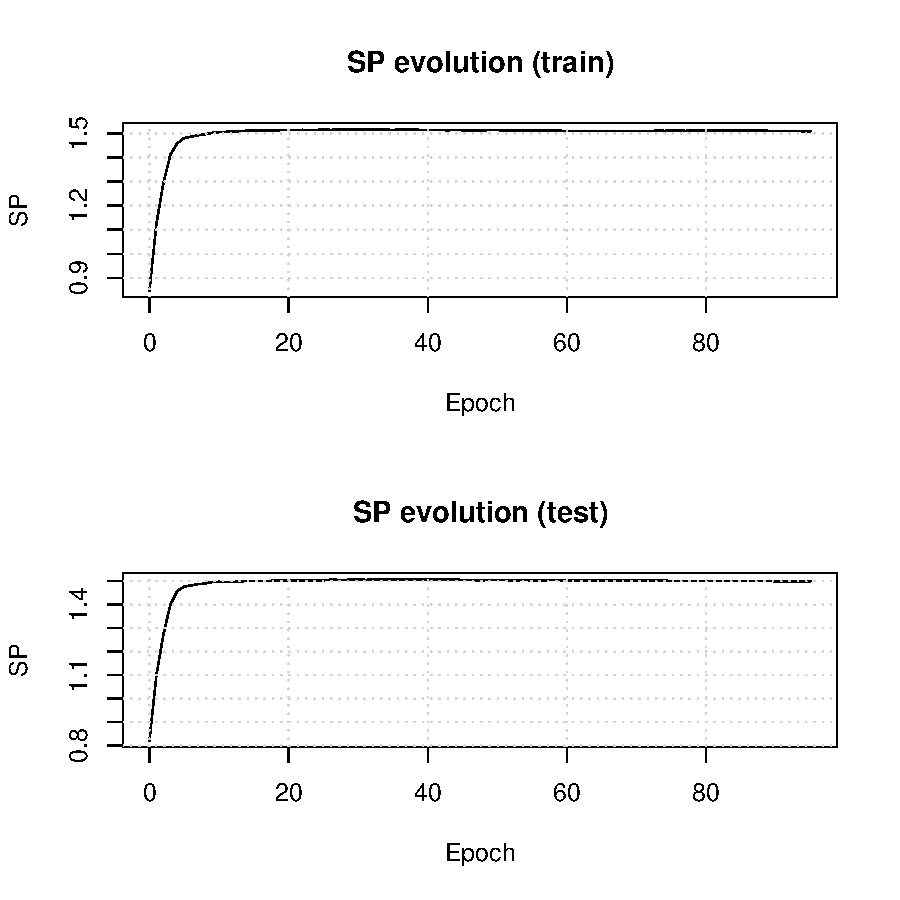
\includegraphics[scale=0.98]{lms/sp-evolution}
\end{center}
\caption{Evolução dos valores do produto SP ao longo do treinamento do detetor
LMS, para o conjunto de treinamento (topo) e de teste (embaixo). A taxa de
treinamento para este sistema é $0,01$ equanto que o tamanho da época
escolhido é $500$.}
\label{fig:lms-sp-evo}
\end{figure}

A Figura~\ref{fig:lms-test-output} mostra os histogramas da saída da rede para
elétrons (alto) e jatos (embaixo), considerando-se o conjunto de teste. O
ponto ótimo de corte, determinado para que se maximize o produto SP da rede
para o conjunto de treinamento para este sistema é $-0,0473$. Nestas
condições, o máximo produto SP para o conjunto de teste é 1,51, definido no
ponto da curva R.O.C. (veja Figura~\ref{fig:lms-test-roc}) onde a eficiência
para a deteção de elétrons é 91,64\% enquanto que a eficiência para a deteção
de jatos é de 90,35\%. A Figura~\ref{fig:lms-vs-egamma-roc} mostra uma
comparativo entre o resultado da otimização proposta atualmente no experimento
ATLAS contra os resultados obtidos para este classificador. Através desta
figura é possível observar que o discriminador LMS tangencia a parte exterior
dos pontos da otimização proposta atualmente no experimento. O resultado
obtido com o algoritmo LMS, ao invés do longo processo de otimização proposto
originalmente, é atingido depois de apenas 1 minuto e 30 segundos de
treinamento em um computador dotado de um processador AMD 64 com \eng{clock}
de 2~GHz e 1~Gb de memória RAM. Ademais, tal sistema apresenta uma capacidade
discriminatória praticamente ótima após apenas 20 passos de treinamentos, isto
é, $\approx 25$ segundos na máquina citada.

\begin{figure}
\begin{center}
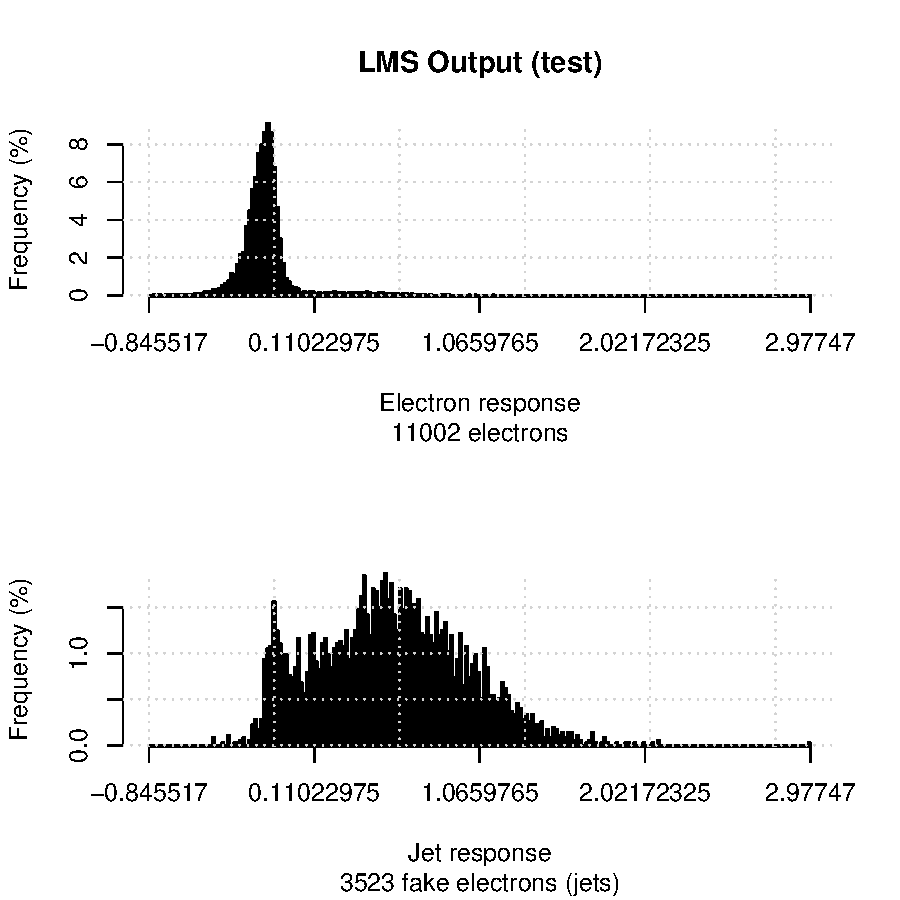
\includegraphics[scale=0.98]{lms/test-output}
\end{center}
\caption{Saída do detetor LMS em estudo para o conjunto de treino.}
\label{fig:lms-test-output}
\end{figure}

\begin{figure}
\begin{center}
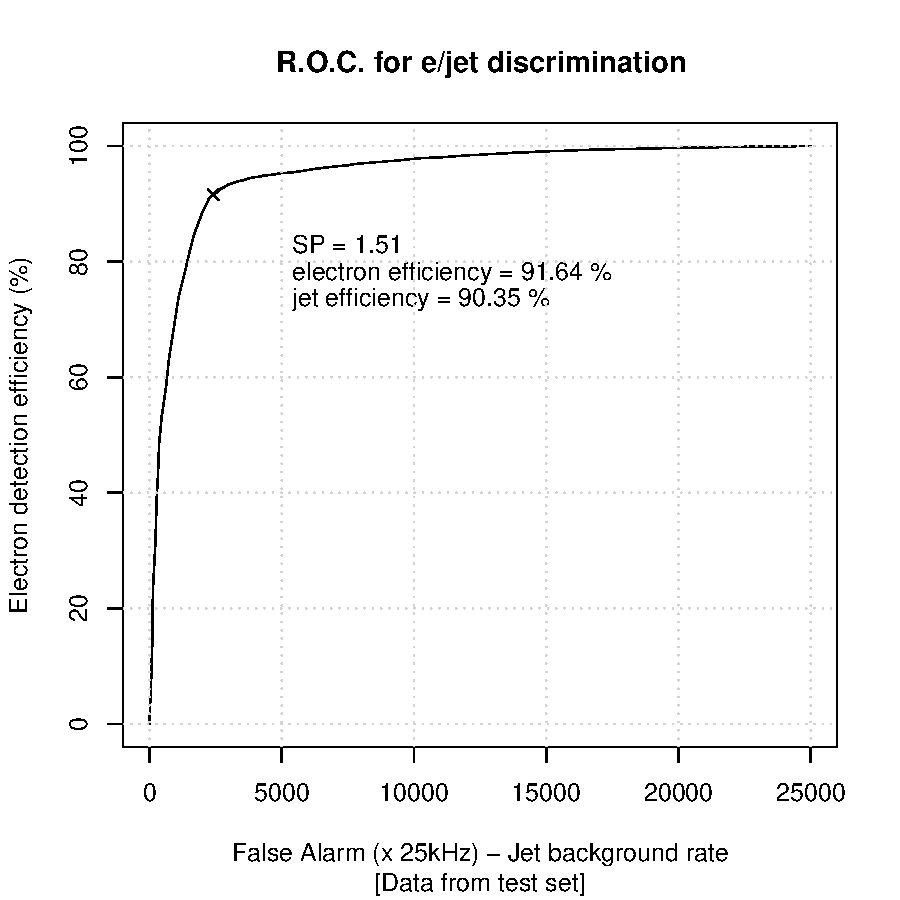
\includegraphics[scale=0.98]{lms/test-roc}
\end{center}
\caption{Curva R.O.C. para um detetor elétron/jato baseado no detetor LMS em
estudo.}
\label{fig:lms-test-roc}
\end{figure}

\begin{figure}
\begin{center}
\includegraphics[scale=0.98]{lms/lms-vs-egamma-roc}
\end{center}
\caption{R.O.Cs comparativas entre a otimização atual para o EGammaHypo e um
detetor baseado no LMS.}
\label{fig:lms-vs-egamma-roc}
\end{figure}

As Figuras~\ref{fig:lms-test-sp-eta}, \ref{fig:lms-test-sp-phi} e
\ref{fig:lms-test-sp-emet} mostram, respectivamente, o valor do produto SP segundo
a distribuição dos dados em $\eta$, $\phi$ e $\etem$. O número anexo ao topo
de cada barra indica a quantidade de cada canal e é útil para que se considere
a relevância de um valor parcial no desempenho do discriminador. Nota-se que
na distribuição por $\eta$, há uma clara perda de eficiência na região
$|\eta| \approx 1,5$. Esta notável queda no desempenho do classificador é
devido a um espaço sem elementos de deteção nesta área (também conhecido como
\eng{gap} ou \eng{crack} dos calorímetros), por onde passam os cabos de
leitura e manutenção dos detetores internos. A eficiência é recuperada logo
após esta região. O gráfico de barras para a distribuição $\phi$ mostra-se
praticamente uniforme, indicando que o sistema funciona sem tendências para
todos os valores desta variável. Este resultado é esperado, já que o detetor é
simétrico neste eixo. A análise por $\etem$ demonstra uma predominante
qualidade de deteção para valores mais baixos de energia que valores mais
altos. Deve-se levar em conta que, embora a eficiência de deteção de elétrons
ainda seja máxima nesta última região, como mostra a
Figura~\ref{fig:lms-test-efficiency-emet}, o falso alarme na deteção de jatos
também apresenta-se máximo. Uma vez que o produto SP é uma figura de mérito da
eficiência agregada de ambas as classes de eventos do discriminador, ela
quantificar-se-á em zero nesta região. Este resultado está associado a baixa
estatística de dados disponível na região.

\begin{figure}
\begin{center}
\includegraphics[scale=0.98]{lms/test-sp-eta}
\end{center}
\caption{Análise do produto SP do detetor LMS, para os dados do conjunto de
teste ao longo de $\eta$.}
\label{fig:lms-test-sp-eta}
\end{figure}

\begin{figure}
\begin{center}
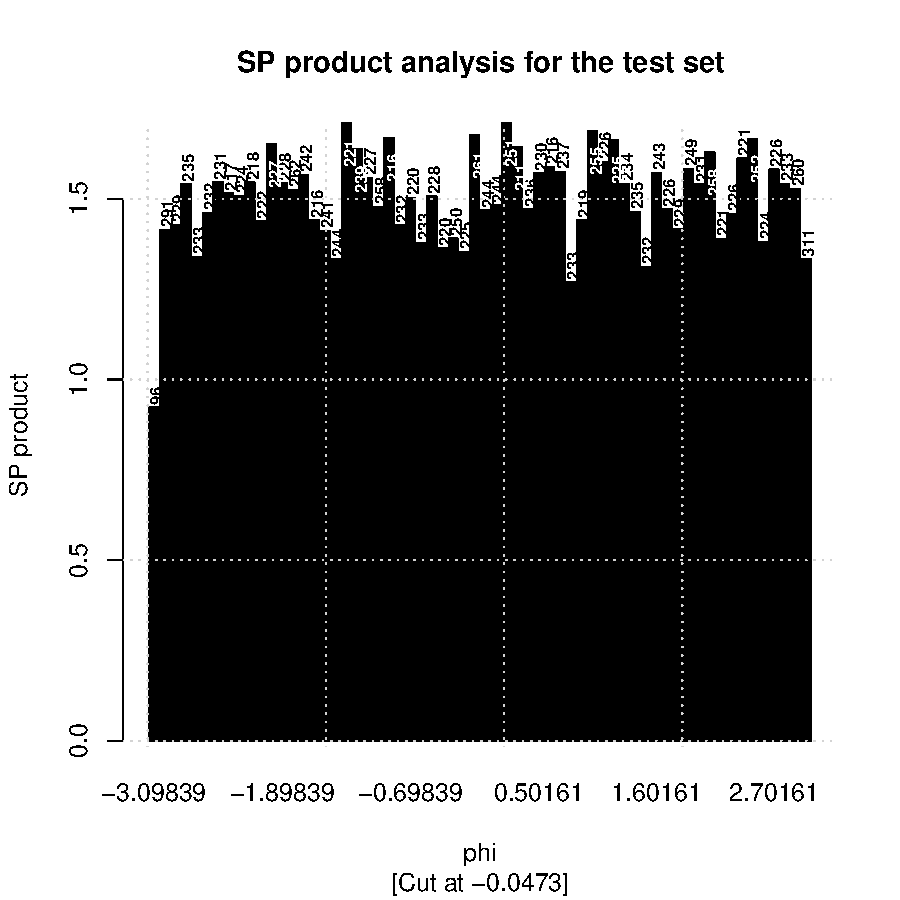
\includegraphics[scale=0.98]{lms/test-sp-phi}
\end{center}
\caption{Análise do produto SP do detetor LMS, para os dados do conjunto de
teste ao longo de $\phi$.} 
\label{fig:lms-test-sp-phi}
\end{figure}

\begin{figure}
\begin{center}
\includegraphics[scale=0.98]{lms/test-sp-emet}
\end{center}
\caption{Análise do produto SP do detetor LMS, para os dados do conjunto de
teste por $\etem$.} 
\label{fig:lms-test-sp-emet}
\end{figure}

\begin{figure}
\begin{center}
\includegraphics[scale=0.98]{lms/test-efficiency-emet}
\end{center}
\caption{Análise da eficiência de deteção de elétrons e falso alarme em jatos
para o detetor LMS, utilizando os dados do conjunto de teste, por $\etem$.}
\label{fig:lms-test-efficiency-emet}
\end{figure}

A Figura~\ref{fig:lms-vs-egamma} mostra um comparativo entre as duas técnicas
de deteção, por energia transversa na seção e.m.. Distingue-se que os dois
sistemas possuem respostas bastante próximas. Na primeira (mais à esquerda)
faixa de energia considerada, o EGammaHypo possui uma resposta melhor enquanto
que com o aumento da energia transversa o LMS apresenta-se mais eficiente, e
segue este padrão para quase todas as faixas consideradas, principalmente onde
há maior concentração de eventos de teste, como é possível determinar à partir
da Figura~\ref{fig:lms-test-sp-emet}.

\begin{figure}
\begin{center}
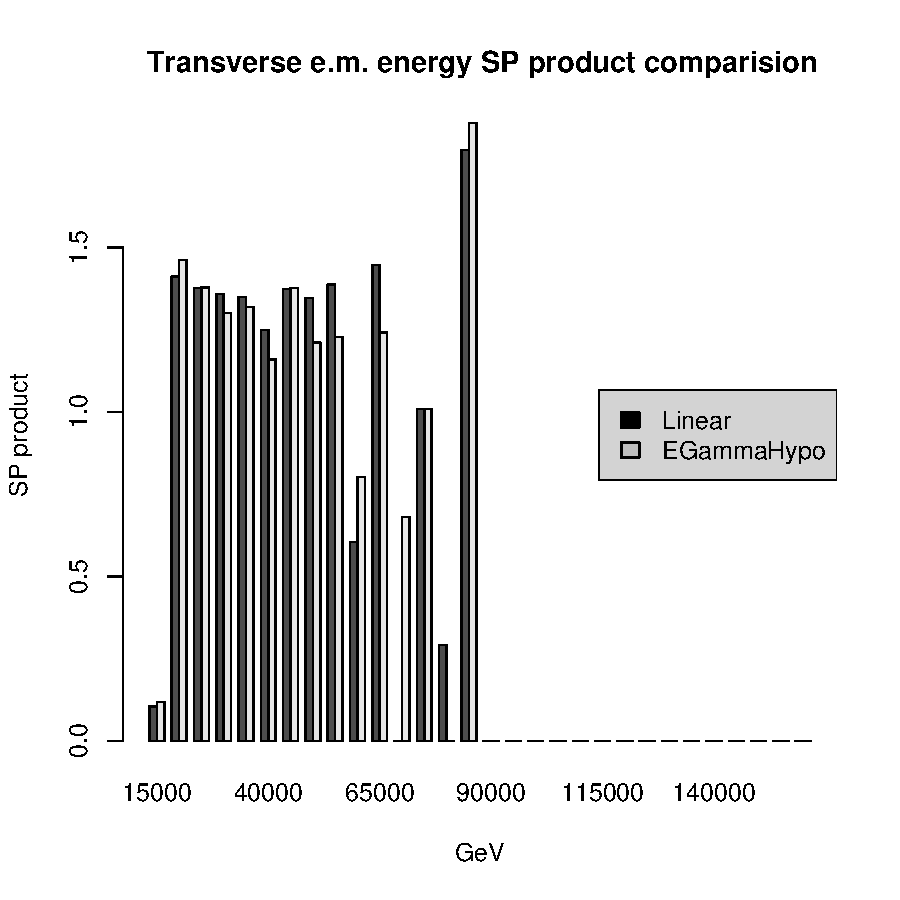
\includegraphics[scale=0.98]{lms/lms-vs-egamma}
\end{center}
\caption{Comparação do produto SP para um classificador baseado no LMS e o
EGammaHypo por energia transversa na seção e.m..}
\label{fig:lms-vs-egamma}
\end{figure}

\subsection{Relevância das características do T2Calo}

A técnica da análise de relevância \cite{relevance} tem por objetivo medir a
importância de cada uma das variáveis de entrada para um classificador. Nesta
técnica, suprime-se a contribuição da variável à composição da saída
substituindo-se seu valor, a cada evento, por sua média, para todos os eventos
disponíveis na entrada do sistema de discriminação. Observando-se a variação
da saída, é possível estimar a contribuição daquela variável ao processo
discriminatório. A estimativa de relevância da i-ésima componente de entrada
pode, então ser calculada pela fórmula:

\begin{equation}
R_i = \frac{1}{N} \text{ } \overset{N}{\underset{j=1}{\sum}} \text{ }
[\text{saída}(\overrightarrow{x_j}) -
\text{saída}(\overrightarrow{x_j}\mid_{x_{j,i} = \overline{x}_i})]^2 
\label{eq:relevance-mse}
\end{equation}

Em outras palavras, é possível definir a relevância da variável $x_i$, $R_i$,
como o EMQ da saída de um discriminador comparada a mesma saída quando faz-se
a variável assumir o valor de sua média. Nessa equação, $N$ representa o
número total de eventos (padrões) disponíveis para o classificador. A
Figura~\ref{fig:relevance-mse} mostra os valores de relevância para cada uma
das variáveis do classificador em análise. Esta figura mostra, mais uma vez,
que o conjunto de treino permite generalizar o comportamento do discriminador,
apresentando valores de relevância, para cada uma de suas variáveis, bastante
próximos daqueles valores calculados para o conjunto de teste. Esta figura
também mostra que a variável $\rcore$ é de extrema importância na determinação
da saída do detetor. Quando substituímo-la por sua média, o erro na saída
aumenta de mais de 3 pontos enquanto que para as demais variáveis, o impacto é
nitidamente menor. Esta figura também indica que a ordem de separação proposta
pelo EGammaHypo está em acordo com o processo de filtragem definido
automaticamente pelo LMS, levando-se em consideração a ordem onde os cortes
são aplicados por aquele algoritmo e a importância das variáveis nesse
processo de classificação. A importância destas variáveis ao sistema LMS
poderia ser utilizada para simplificá-lo. Por exemplo, seria possível
``podar'' a variável menos relevante e re-treinar o sistema para obter um
classificador mais rápido.

\begin{figure}
\begin{center}
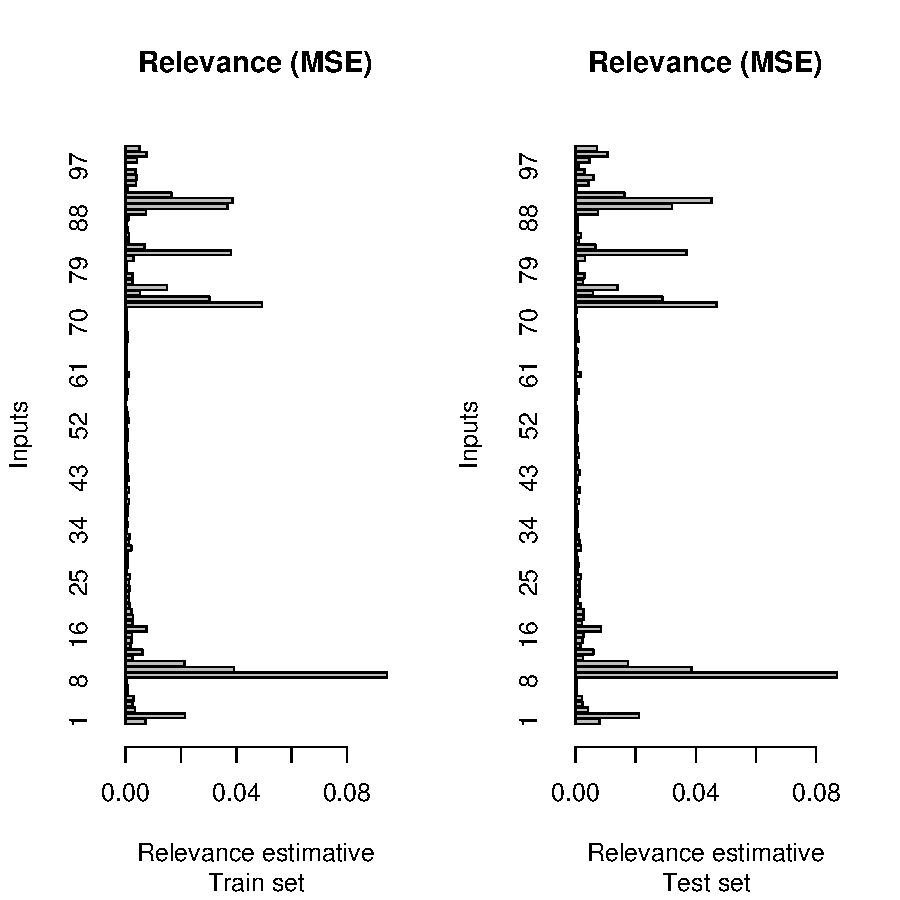
\includegraphics[scale=0.98]{lms/relevance-mse}
\end{center}
\caption{Os valores de relevância para os conjunto de treino (cinza claro) e
teste (em cinza escuro), para as 4 variáveis do T2Calo e considerando-se o
classificador LMS em estudo.}
\label{fig:relevance-mse}
\end{figure}

Por outro lado, como foi visto nas análises de evolução do EMQ
(Figura~\ref{fig:lms-mse-evo}) e do produto SP (Figura~\ref{fig:lms-sp-evo}),
a capacidade discriminatória da rede reage de forma correlacionada, mas
\textbf{não necessariamente} idêntica ao processo de mapeamento da entrada
na saída proposto pelo LMS. Observa-se que, apesar de notarmos uma contínua
migração ao mínimo EMQ durante cerca de 100 passos de treinamento, após cerca
de apenas 20 passos, a capacidade discriminatória do sistema já atinge seu
máximo e ali permanece até o final do treinamento. Este comportamento indica
que exista uma diferença não-negligível entre estes dois parâmetros. Desta
forma, propõe-se uma variação do cálculo da relevância, mas agora baseando-se
no impacto da substituição do valor da variável pela sua média à capacidade
discriminatória da rede, agora representada pela variação do produto SP, da
seguinte forma:

\begin{equation}
R_{d_i} = \max(\text{SP}_{\text{original}}) - \max(\text{SP}(\overrightarrow{x_j}\mid_{x_{j,i} = \overline{x}_i}))
\label{eq:relevance-sp}
\end{equation}

Neste caso define-se a relevância $R_{d_i}$ da variável $i$ como a diferença
no produto SP máximo causado pela substituição desta variável pela sua
média. De fato, espera-se que a maior parte dos valores de relevância sejam
positivos, indicando uma degradação do desempenho do classificador seguindo a
neutralização de uma variável. Seria possível que se encontrasee valores de
relevância negativos, o que indicaria que uma variável está, na verdade,
atrapalhando o processo de classificação ao invés de melhorá-lo. A
Figura~\ref{fig:relevance-sp} mostra os valores de $R_d$ para o classificador
LMS em estudo. Como é possível ver nesta figura, o quadro é marginalmente
diferente daquele mostrado pela Figura~\ref{fig:relevance-mse}. A variável
mais importante para o processo discriminatório é ainda $\rcore$, seguindo-se
de $\eratio$ e $\ethad$. A variável $\etem$ é a menos relevante para o
processo de classificação de elétrons e jatos, o que já era esperado
observando-se as tendências com o EGammaHypo. Como é possível definir à partir
deste gráfico, seria preferencial uma poda da variável $\etem$ que da variável
$\ethad$, como sugeriria a Figura~\ref{fig:relevance-mse}. No mais, as duas
figuras são bastante compatíveis e indicam uma tendência importante: a
minimização do EMQ também maximizará o produto SP. Esta figura também
indicaria que a ordem na qual o EGammaHypo considera as variáveis de corte
(i.e. $\rcore \rightarrow
\eratio \rightarrow \etem \rightarrow \ethad$) seja não-ótima para o conjunto
de dados sendo analisado, mesmo que marginalmente. Observa-se que seria mais
interessante que o corte em $\etem$ fosse realizado por último ao invés do
corte em $\ethad$, pois desta forma o processo discriminatório seria mais
rápido.

\begin{figure}
\begin{center}
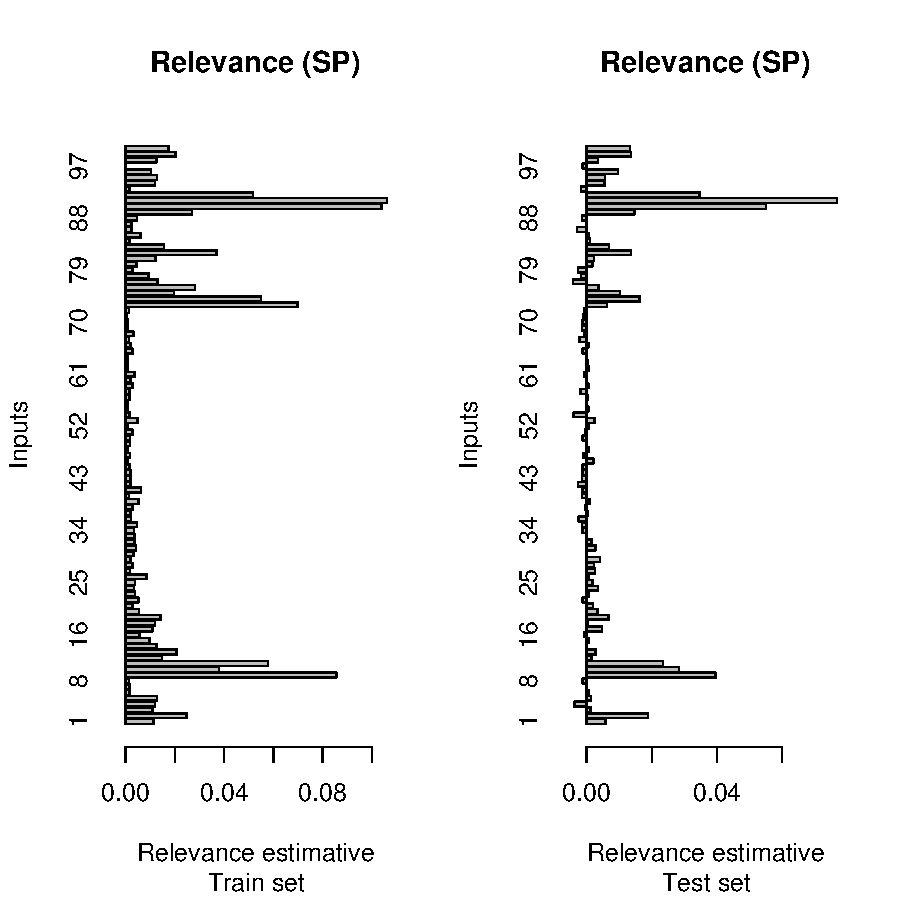
\includegraphics[scale=0.98]{lms/relevance-sp}
\end{center}
\caption{Os valores de relevância de discriminação para os conjunto de treino
(cinza claro) e teste (em cinza escuro), para as 4 variáveis do T2Calo e
considerando-se o classificador LMS em estudo.}
\label{fig:relevance-sp}
\end{figure}

\section{Métodos neurais de discriminação}
\label{sec:neural}

Redes neurais artificiais (RNA) vêm sendo atualmente utilizadas com sucesso em
problemas de otimização, controle e reconhecimento de padrões
\cite{haykin}. RNA's são modelos matemáticos inspirados no conhecimento
limitado que temos do cérebro animal. Neste contexto, entende-se que uma rede
neural pode aprender através do contato com os elementos de interesse de um
determinado espaço de entrada e que este conhecimento é armazenado através das
conexões sinápticas que conectam os elementos processadores (neurônios) da
rede. Dentre as características de uma RNA podemos destacar:

\begin{description}
\item[Robustez] Em ambientes extremamente \emph{agressivos} (sujeitos a falhas
e a radioatividade), como é o caso da operação do ATLAS, RNA's podem manter um
excelente desempenho, mesmo quando parte dos dados (canais de aquisição) de
entrada são perdidos;

\item[Generalização] RNA's podem extrair a informação relevante escondida sob
uma grande quantidade de ruído;

\item[Deteção de novos fenômenos] RNA's podem detetar a ocorrência de novos
objetos de forma bastante eficaz. Isto é \underline{extremamente} importante
em ambientes que podem revelar resultados inesperados (nova física);

\item[Simples implementação] RNA's podem ser facilmente descritas em
linguagens de programação convencionais, atingindo desempenhos satisfatórios
para um grande conjunto de aplicações em tempo real.
\end{description}

A utilização de RNA's em experimentos em Física de Altas Energias também vem
se popularizando ao longo das últimas década, principalmente na área de
calorimetria, tanto especificamente em sistemas de filtragem \cite{badgett92,
koehne96} quanto para análise pós-reconstrução \cite{altherr90}. Isto se deve
principalmente ao fato que RNA's consigam definir uma superfície de separação
não-linear no espaço de dados sendo considerado, normalmente atingindo
resultados bastante acurados na determinação do \eng{background} e ainda
retendo um desempenho satisfatório quando comparadas às técnicas de deteção
por cortes como as discutidas anteriormente (veja a
Seção~\ref{sec:def-eghypo}).

\subsection{Introdução ao processamento neural}

A Figura~\ref{fig:neuron} contém uma modelagem de um neurônio
genérico. Analogamente ao sistema LMS descrito na Seção~\ref{sec:lms}, os
elementos processadores de uma rede neural, chamados neurônios ou percéptrons,
são ativados por um conjunto de entradas $\overrightarrow{x}$, somadas de
acordo com um sistema linear de ponderação $\overrightarrow{w}$. O diferencial
entre o sistema linear proposto anteriormente e um neurônio está na função de
ativação que conduz o campo induzido $v_p =
\overrightarrow{x}*\overrightarrow{w}_{p}^{T}$ à saída. Enquanto que
no caso do LMS utiliza-se a função identidade, i.e., $y_p = v_p$, no caso de
percéptrons, faz-se uso de uma função não-linear, como por exemplo a função
tangente hiperbólica:

\begin{figure}
\begin{center}
\includegraphics{neuron}
\end{center}
\caption{Grafo de fluxo de sinal de um neurônio artificial.}
\label{fig:neuron}
\end{figure}

\begin{equation}
tanh(v) = \frac{e^v - e^{-v}}{e^v + e^{-v}} = \frac{e^{2v} - 1}{e^{2v} + 1}
\label{eq:tanh}
\end{equation}

Ou a função logística (simplificada):

\begin{equation}
P(v) = \frac{1}{1 + e^{-v}}
\label{eq:logf}
\end{equation}

A razão da escolha de uma função não-linear para a ativação de um campo
induzido pode ser qualificado à partir da seguinte constatação: se sistema a
que se deseja classificar aprensenta um comportamento gaussiano, para ambas as
classes, i.e., os momentos de ordem superior a $2$ para ambas as classes são
todos iguais a zero, o classificador ótimo (bayesiano) resume-se um sistema
linear \cite{haykin}. Naturalmente nota-se que seja sempre possível
\textit{aproximar} ou modelar um sistema não-gaussiano em um desta espécie,
tendo por conseqüência os erros relativos a esta aproximação. De fato, foi o
que foi realizado na Seção~\ref{sec:lms-ej}, quando escolhou-se utilizar um
classificador linear para separar as quatro variáveis definidas pelo T2Calo.

Se o sistema que se deseja resolver apresenta um comportamento não-gaussiano,
o classificador ótimo não pode ser representando por um classificador
linear. Neste caso, utiliza-se uma função de ativação não-linear para que se
aproxime, de alguma forma, o comportamento não-linear do sistema de interesse.
As funções nas Equações~(\ref{eq:tanh}) e (\ref{eq:logf}) são normalmente
utilizadas por apresentarem amplitude limitada e possuírem derivada
trivialmente calculável. A razão de procurar-se funções com derivadas simples
(e suaves) ficará mais clara adiante, quando se definir o algoritmo de
treinamento. A amplitude limitada pode rapidamente ser verificada como uma
característica de interesse observando-se que o treinamento de um sistema que
trabalha por aprendizado seja muitas vezes executado com a retro-alimentação
de erros. Neste caso, para evitar oscilações e pontos de ressonância, um
sistema cuja a saída seja limitada apresenta natural vantagem se comparado a
outro análogo \cite{haykin}.

Este estudo está focado na utilização de RNA's utilizando percéptrons em
múltiplas camadas (do inglês \eng{Multi-layer perceptrons} ou MLP),
completamente conectadas, sem realimentação e com treinamento baseado na
retropropagação de erros. Introduziremos o processo de treinamento destes
sistemas à seguir.

\subsection{Treinamento por retro-propagação de erros}

Para sistemas com apenas uma camada neural, observa-se que, ao buscar-se o
ponto de mínimo da superfície de erro (quadrático), naturalmente otimiza-se o
conjunto de pesos de tal forma que o sistema consiga mapear a entrada nos
alvos de saída. A única restrição do método é que a função de ativação do
campo induzido do neurônio $\varphi(\cdot)$ seja diferenciável.
\cite{rosenblatt}. O problema do treinamento de uma rede MLP é um pouco mais
complexo. Um grafo de fluxo de uma rede MLP completamente conectada pode ser
visto na Figura~\ref{fig:simple-mlp}. Neste caso considera-se que a rede
possui apenas uma camada escondida e apenas um neurônio de saída pois se
identifica intimamente com os casos de uso que abordaremos. Ainda sim, seria
possível considerar casos com um número maior de neurônios de saída ou com
mais camadas escondidas generalizando os casos exemplificados aqui.

\begin{figure}
\begin{center}
\includegraphics{simple-mlp}
\end{center}
\caption{Modelagem de uma rede MLP, totalmente conectada e sem
retro-propagação de sinal.}
\label{fig:simple-mlp}
\end{figure}

Para o sistema em questão, o mecanismo de treinamento para o neurônio de saída
é idêntico ao treinamento de um percéptron simples, e pode ser facilmente
definido da seguinte forma:

\begin{align}
\text{Se define-se o erro como } \mathcal{E}(n) &= \frac{1}{2}e_{k}^{2}(n)
\label{eq:error-def} \\
\text{e considerando-se que } \frac{\partial\mathcal{E}(n)}{\partial
w_{jk}(n)} &= \frac{\partial\mathcal{E}(n)}{\partial e_k(n)} \frac{\partial
e_k(n)}{\partial y_k(n)} \frac{\partial y_k(n)}{\partial v_k(n)}
\frac{\partial v_k(n)}{\partial w_{jk}(n)} \label{eq:partials} \\
\text{ou seja, } \frac{\partial\mathcal{E}(n)}{\partial
w_{jk}(n)} &= e_k(n)(-1)\varphi_{k}'(v_{k}(n))y_{k}(n)
\label{eq:partials-solution} \\
\text{e, resumindo, } \Delta w_{jk}(n) &=
-\eta\frac{\partial\mathcal{E}(n)}{\partial w_{jk}(n)} = \eta
e_{k}(n)\varphi_{k}'(v_{k}(n))y_{k}(n)
\end{align}

Normalmente, define-se:

\begin{align}
\text{Gradiente local: } \delta_k(n) &= - e_k(n)\varphi_{k}'(v_k(n)) \\
\text{e desta forma } \Delta w_{jk}(n) &= \eta\delta_k(n)y_{k}(n)
\label{eq:neural-train}
\end{align}

Este sistema de equações segue o princípio definido anteriormente para o LMS,
mas sem assumir nada sobre a função de ativação $\varphi(\cdot)$. Nota-se que
para uma função de ativação onde $y_k(n) = v_k(n)$, recai-se no algoritmo de
treinamento do LMS: $\Delta w_{jk}(n) = \eta e_{j}(n)y_{j}(n)$. Desta forma, é
possível considerar o LMS como um caso especial de uma rede neural com apenas
uma camada e cuja a função de ativação é a função identidade. Nestas equações,
$n$ representa a época ou batelada de treinamento.

O segundo caso de interesse acontece quando o neurônio $j$ está localizado em
uma camada oculta da rede. Neste caso, não existe uma resposta desejada (alvo)
específica para aquele neurônio. Desta forma, tentar-se-á definir o sinal de
erro de um neurônio escondido recursivamente, através da retro-propagação do
erro na saída final da rede em direção ao neurônio desejado. Iniciamos,
intuitivamente, com a definição do gradiente local do neurônio escondido $j$:

\begin{equation}
\delta_j(n) = -\frac{\partial\mathcal{E}(n)}{\partial
v_j(n)} = -\frac{\partial\mathcal{E}(n)}{\partial
y_j(n)}\frac{\partial y_j(n)}{\partial v_j(n)} =
-\frac{\partial\mathcal{E}(n)}{\partial y_j(n)}\varphi_{j}'(v_j(n))
\end{equation}

Tendo em conta, que para o caso específico em análise:

\begin{align}
\mathcal{E}(n) &= \frac{1}{2}e_{k}^{2}(n) \\
\text{conclui-se que } \frac{\partial\mathcal{E}(n)}{\partial y_j(n)} &=
e_{k}\frac{\partial e_k(n)}{\partial y_j(n)} = e_{k}\frac{\partial
e_k(n)}{\partial v_k(n)}\frac{\partial v_k(n)}{\partial y_j(n)}
\end{align}

A primeira derivada parcial, $\partial e_k(n)/\partial v_k(n)$, já foi
calculada para o caso do neurônio de saída, na passagem da
Equação~(\ref{eq:partials}) para a
Equação~(\ref{eq:partials-solution}). Utiliza-se a mesma analogia aqui. Para o
cálculo da segunda derivada parcial, pela Figura~\ref{fig:simple-mlp}
deduz-se que:

\begin{align}
v_k(n) &= \sum_{j} w_{jk}(n)y_j(n) \\
\text{e, portanto: } \frac{\partial v_k(n)}{\partial y_j(n)} &= w_{jk}(n)
\end{align}

Assim sendo, o gradiente local do neurônio escondido $j$ assim se define:

\begin{equation}
\delta_j(n) = \varphi_{j}'(v_j(n))\delta_k(n)w_{jk}(n)
\label{eq:local-gradient-hidden}
\end{equation}

Substituindo $\delta_j(n)$ na Equação~(\ref{eq:neural-train}), chega-se a
fórmula de treinamento do neurônio escondido. No caso onde há muitas saídas na
rede, a Equação~(\ref{eq:local-gradient-hidden}) é trivialmente redefinida da
seguinte forma: 

\begin{equation}
\delta_j(n) = \varphi_{j}'(v_j(n))\sum_{k}\delta_k(n)w_{jk}(n)
\label{eq:local-gradient-hidden-multi}
\end{equation}

No caso em que existem múltiplas camadas escondidas, propaga-se recursivamente
o erro em direção à camada de entrada, aplicando-se a
Equação~(\ref{eq:local-gradient-hidden-multi}). 

\subsubsection{Funções de ativação} 

A função de ativação $\varphi(\cdot)$ deve ser diferenciável em toda a
extensão do domínio de interesse. No entanto, para simplificar o cálculo
computacional dos gradientes locais, é habitual a escolha de funções que
possuam um cálculo trival de suas derivadas. Como exemplo, foram citadas as
funções tangente hiperbólica (Equação~\ref{eq:tanh}) e a função logística
simplificada (Equação~\ref{eq:logf}). No caso da função logística:

\begin{align}
\varphi(z) &= \frac{1}{1 + e^{-z}} \\
\text{Daí } \varphi'(z) &= \frac{e^{-z}}{[1+e^{-z}]^2}
\end{align}

Levando-se em consideração que para um neurônio genérico $y =
\varphi(v)$. Então:

\begin{equation}
\varphi'(v) = \frac{e^{-v}}{[1+e^{-v}]^2} = \frac{1+e^{-v}}{[1+e^{-v}]^2} -
\frac{1}{[1+e^{-v}]^2} = \varphi(v)[1 - \varphi(v)] = y(1-y)
\end{equation}

No caso da tangente hiperbólica, equivalentemente:

\begin{align}
\varphi(z) &= \tanh(z) \\
\varphi'(z) &= \text(sech)^2(z) = 1 - \tanh^2(z) \\
\varphi'(v(n)) &= 1 - \varphi^2(z) = 1-y^2(n)
\end{align}

Estas duas funções de ativação permitem um cálculo absolutamente trivial do
gradiente local e por esta razão são computacionalmente bastante
eficientes. No decorrer deste estudo utilizaremos a função tangente
hiperbólica com função de ativação dos percéptrons das redes estudadas.

\subsubsection{Convergência}

O algoritmo de retropropagação usa uma estimativa instantânea do gradiente da
superfície de erro no espaço dos pesos. Por esta razão, este sistema possui
uma inerente natureza estocástica e tende a oscilar ao redor da direção de
convergência ótima, ao mínimo da função de erro. Isso acontece pois é difícil
antever se inclinações demasiado bruscas ou suaves em uma das direções da
superfície de erro não influenciarão excessivamente o deslocamento do
sistema. Muitas vezes, a utilização de um amortecimento (ou \emph{momento})
durante o treinamento pode melhorar a resposta do sistema. Utiliza-se esta
técnica para suavizar a migração das redes em direção ao mínimo da superfície
de erro. Outra técnica é a normalização dos dados de entrada da rede, de forma
que se evite que a diferença de magnitude e variabilidade das componentes de
entrada cause tendências no treinamento neural.

Um problema recorrente no treinamento de redes neurais são mínimos locais, que
podem fazer com que o sistema fique ``preso'' em uma região que não represente
o mínimo global da superfície de erro. Esta característica não é somente mais
uma conseqüência da utilização da estimativa instantânea para definir a
direção de movimentação dos pesos, mas muitas vezes ocorre por dispor-se de
uma quantidade limitada de eventos que representem o fenômeno que se deseja
mapear.

Para que se assegure de que o sistema convirja sempre a um patamar equivalente
de mínimo, deve se realizar um número de experimentos com os mesmos parâmetros
de treinamento e teste para todos os casos de estudo. Em cada teste
inicializa-se os pesos sinápticos à partir de um ponto diferente da superfície
de erro. Desta forma, será possível detetar e avaliar se o problema em estudo
estará sujeito a mínimos locais.

\subsection{Discriminação neural aplicada às saídas do T2Calo}

É possível substituir o discriminador LMS definido na Seção{sec:lms} por um
discriminador baseado em uma rede neural tipo MLP como a da
Figura~\ref{fig:simple-mlp}. A implementação desta rede neural encontra-se bem
detalhada no Apêndice\ref{ap:framework} e é facilmente implementável usando
o pacote \eng{NeuralRinger} e o fluxo de treinamento detalhado na
Figura~\ref{fig:train-flow}. A Figura~\ref{fig:t2calo-neural} contém um
diagrama de blocos que ilustra, de forma simplificada, tal sistema. Os fatores
de normalização empregados para o sistema de deteção baseado no algoritmo LMS
não precisam ser substituídos, já que deseja-se empregar o mesmo tipo de
normalização antes de alimentarmos o sistema neural com os dados disponíveis,
a fim de evitar qualquer tipo de tendência devida à variância ou média dos
dados. Os conjuntos de treinamento e teste serão mantidos, o que simplificará
a comparação das duas técnicas.

\begin{figure}
\begin{center}
\includegraphics[scale=1]{t2calo-neural}
\end{center}
\caption{Um discriminador neural para as características definidas pelo
T2Calo.}
\label{fig:t2calo-neural}
\end{figure}

Neste novo sistema neural um conjunto maior de parâmetros de treinamento
estará disponível e torna-se necessária a avaliação destes em função do tempo
e qualidade de treinamento das redes. Estes parâmetros são:

\begin{itemize}
\item Taxa de aprendizagem da rede;
\item Tamanho da época;
\item Número de neurônios na camada escondida\footnote{Este estudo
limita-se a utilização de Redes Neurais artificiais com uma única camada
escondida.};
\item Momento.
\end{itemize}

A utilização de um valor de momento tem por objetivo amortecer o treinamento
de forma que a migração para o mínimo da superfície de erro ocorra de forma
suave, e será empregado no caso de observarmos que o treinamento comporta-se
de forma oscilatória. Para cada uma destas variáveis, define-se um conjunto de
sub-valores de interesse:

\begin{itemize}
\item Taxa de aprendizagem: $[0,001; 0,002; 0,005; 0,01; 0,02; 0,05; 0,1;
0,15]$;
\item Tamanho da época: $[50; 100; 200; 500; 1000; 1500]$;
\item Neurônios escondidos: $[2; 3; 4; 5; 6]$;
\item Momento: $[0; 0,01; 0,02; 0,05; 0,1; 0,2]$.
\end{itemize}

Cada conjunto individual de parâmetros deve ser avaliado em função de um
número considerável de pontos de inicialização dos pesos sinápticos da rede
neural. Deseja-se assegurar que as redes convirjam à pontos próximos (se não
idênticos) na superfície de erro considerada, independentemente de sua
inicialização. Estipulou-se que o número de testes para cada conjunto de
parâmetros será 5. Ou seja, para cada ponto no espaço de otimização do
treinamento, conduziremos 5 testes inicializando os pesos sinápticos com
valores aleatórios distintos e disparando o treinamento. Considerar-se-á os
máximos e mínimos obtidos no produto SP do classificador, para o conjunto de
teste, na avaliação de seu desempenho.

Uma inspeção rápida do número de testes a serem executados mostra que, para
este conjunto de parâmetros, cerca de ($8\times6\times5\times6\times5$) 
$7200$ testes devem ser realizados. Embora tentador, este cenário aparenta-se
mais complexo que o problema inicial da otimização do EGammaHypo, com uma
desvantagem: o número de parâmetros aumentou. Uma avaliação mais detalhada da
natureza do espaço de otimização pode ser benéfica a simplificação deste
processo: 

\begin{itemize}
\item Numa análise inicial, é possível suprimir a variação do momento, já que
a contribuição desejada deste parâmetro está no amortecimento do
treinamento. Seria possível adotar a seguinte estratégia: inicialmente
identifica-se a melhor taxa de aprendizagem. Em seguida, estuda-se como
aplicar o momento de forma que o discriminador final seja treinado evitando
transições abruptas do MSE ou do produto SP;

\item O número de neurônios escondidos poderia ser, inicialmente fixado em 4,
igualando o número de entradas. Reconhece-se que um sistema com menos
neurônios escondidos possa apresentar a mesma eficiência ou ainda que um
sistema com mais, convirja mais suavemente. Ainda sim, espera-se que as
tendências no tocante aos outros parâmetros de otimização sejam preservadas e
seja possível identificar o número ótimo de neurônios na camada escondida de
forma \textit{quasi}-independente ao restante dos valores;

\item O tamanho da época pode ser fixado baseando-se na experiência inicial
com o discriminador LMS. O valor utilizado para aquele sistema foi de 500
eventos por época.
\end{itemize}

Desta forma, propõe-se a seguinte heurística de otimização:

\begin{enumerate}
\item Fixa-se todos os parâmetros de treinamento, variando-se a taxa de
aprendizagem em busca de um ótimo para este parâmetro;
\item De posse da taxa de aprendizagem ótima, varia-se o tamanho da época;
\item O número de neurônios escondidos ótimo poderá então ser analisado tendo
em consideração valores ótimos de taxa de aprendizado e o tamanho da época;
\item Por final, varia-se o momento afim de suavizar ao máximo o treinamento
do detetor neural. A utilização de momento será necessária, \textbf{se e
somente se} o treinamento neural se mostrar excessivamente ruidoso.
\end{enumerate}

\subsubsection{Otimização da taxa de aprendizado}

O primeiro parâmetro a ser otimizado, seguindo a heurística proposta é a taxa
de treinamento. Neste caso, 8 valores estão sendo considerados. Para cada um
dos 8 valores, realizou-se 5 testes onde os pesos sinápticos são inicializados
de forma aleatória e distinta. Para cada conjunto de testes relacionados com
um valor fixo de taxa de treinamento, encontra-se a média e o desvio padrão do
produto SP para os conjuntos de treino e teste e do número de passos de
treinamento. Os resultados desta análise podem ser vistos na
Tabela~\ref{tab:t2calo-neural-lr-scan}. O tamanho da época está fixo em 500, o
que indica que, em todos os casos, o sistema teve acesso a um número maior de
padrões que o total disponível para treinamento (cerca de $14500$ padrões,
incluindo elétrons e jatos).

\begin{table}
\begin{center}
\begin{tabular}{|r|r|r|r|} \hline
Tx. de aprendizado & Passos & Prod. SP (treino) & Prod. SP (teste) \\
\hline 
0.0010 & $1339\pm248$ & $1.4935\pm0.0162$ & $1.4943\pm0.0178$ \\ \hline
0.0020 & $1048\pm407$ & $1.4850\pm0.0108$ & $1.4880\pm0.0107$ \\ \hline
0.0050 & $617\pm229$ & $1.4995\pm0.0163$ & $1.4932\pm0.0147$ \\ \hline
0.0100 & $335\pm51$ & $1.4943\pm0.0074$ & $1.4918\pm0.0059$ \\ \hline
0.0200 & $204\pm36$ & $1.5168\pm0.0127$ & $1.5104\pm0.0139$ \\ \hline
0.0500 & $123\pm21$ & $1.5087\pm0.0123$ & $1.5052\pm0.0134$ \\ \hline
0.1000 & $80\pm21$ & $1.5150\pm0.0067$ & $1.5101\pm0.0055$ \\ \hline
0.1500 & $85\pm28$ & $1.5121\pm0.0046$ & $1.5094\pm0.0032$ \\ \hline
\end{tabular}
\end{center}
\caption{Resultados da otimização da taxa de treinamento para um discriminador
neural elétron/jato baseado na saída do T2Calo.}
\label{tab:t2calo-neural-lr-scan}
\end{table}

A tabela mostra que um valor pequeno de taxa de treinamento faz com que a
duração deste processo se extenda demasiado sem, necessariamente compensar em
melhores resultados. Em todos os casos, o sistema parece sempre convergir para
um máximo próximo à 1,50 de produto SP (considerando valores para o conjunto
de teste). Conforme aumenta-se a taxa de treinamento, o número de passos para
a estabilização do sistema diminui, chegando, no caso em que a taxa é igual a
$0,1$, a necessitar apenas de 80 iterações para a convergência. Uma vez que a
média do produto SP apresenta-se maior para o valor de taxa de treinamento
igual a $0,02$, utilizaremos este valor como o valor padrão nas próximas
etapas de otimização.

\subsubsection{Otimização do tamanho da época}

De posse da taxa de aprendizado, é a vez de otimizar-se o tamanho da época,
inicialmente fixa em 500. Os valores de época para o qual deseja-se
experimentar são: $[50; 100; 200; 500; 1000; 1500]$. O mesmo procedimento
utilizado para a otimização da taxa de treinamento será realizado aqui: cinco
testes são realizados para cada tamanho de época. Os resultados destes testes
encontram-se na Tabela~\ref{tab:t2calo-neural-epoch-scan}.

\begin{table}
\begin{center}
\begin{tabular}{|r|r|r|r|} \hline
Padrões por época & Passos & Prod. SP (treino) & Prod. SP (teste) \\
\hline 
50 & $198\pm44$ & $1.5128\pm0.0190$ & $1.5056\pm0.0168$ \\ \hline
100 & $201\pm53$ & $1.5126\pm0.0070$ & $1.5128\pm0.0138$ \\ \hline
200 & $219\pm65$ & $1.5017\pm0.0100$ & $1.5004\pm0.0129$ \\ \hline
500 & $204\pm36$ & $1.5168\pm0.0127$ & $1.5104\pm0.0139$ \\ \hline
1000 & $212\pm34$ & $1.5202\pm0.0167$ & $1.5188\pm0.0121$ \\ \hline
1500 & $185\pm52$ & $1.5083\pm0.0142$ & $1.5051\pm0.0184$ \\ \hline
\end{tabular}
\end{center}
\caption{Resultados da otimização do tamanho da época para um discriminador
neural elétron/jato baseado na saída do T2Calo.}
\label{tab:t2calo-neural-epoch-scan}
\end{table}

Como mostra a tabela, um tamanho de época de $1000$ padrões maximiza a
capacidade discriminante do sistema. O número de iterações não varia
significativamente o que indica que o tempo de treinamento do sistema não está
diretamente correlacionado ao tamanho da época. Utilizar-se-á o valor de
$1000$ como refência na próxima etapa de otimização.

\subsubsection{Otimização do número de neurônios escondidos}

O número de neurônios na camada escondida é a penúltima ou, possivelmente
última etapa na otimização do classificador neural proposto. Neste caso,
utilizaremos os valores pré-estipulados para os dois outros parâmetros: taxa
de treinamento $=0,02$ e tamanho da época de $1000$ padrões. Os valores de
teste são 2, 3, 4, 5 ou 6 neurônios na camada escondida. Mais uma vez, 5
testes são realizados para cada parâmetro e a média e variância do tempo de
treinamento e dos produtos SP é extraída. A
Tabela~\ref{tab:t2calo-neural-hidden-scan} contém os resultados destes testes.

\begin{table}
\begin{center}
\begin{tabular}{|r|r|r|r|} \hline
Número de neur. escondidos & Passos & Prod. SP (treino) &
Prod. SP (teste) \\ \hline 
2 & $259\pm86$ & $1.5086\pm0.0104$ & $1.5078\pm0.0118$ \\ \hline
3 & $178\pm21$ & $1.4967\pm0.0039$ & $1.4921\pm0.0043$ \\ \hline
4 & $212\pm34$ & $1.5202\pm0.0167$ & $1.5188\pm0.0121$ \\ \hline
5 & $173\pm25$ & $1.4982\pm0.0058$ & $1.4941\pm0.0046$ \\ \hline
6 & $198\pm98$ & $1.5025\pm0.0121$ & $1.4986\pm0.0168$ \\ \hline
\end{tabular}
\end{center}
\caption{Resultados da otimização do número de neurônios na camada escondida
para um discriminador neural elétron/jato baseado na saída do T2Calo.}
\label{tab:t2calo-neural-hidden-scan}
\end{table}

Desta tabela, concluímos que o número ótimo de neurônios na camada escondida
deve ser 4. Uma inspeção no desenvolvimento do EMQ e do produto SP nos testes
com os 3 parâmetros de escolha indica que a migração para o mínimo seja suave
e, portanto não seja necessário a aplicação de momento ou qualquer outra
técnica de suavização do treinamento. Em seguida, para confirmar as escolhas,
treina-se um total de 10 redes com os parâmetros selecionados. Os critérios de
parada utilizados são mantidos. Para nos assegurarmos da estabilidade da rede,
deixa-se que a rede treine ainda por cerca de 100 passos depois do ponto de
estabilidade detetado. A Figura~\ref{fig:best-t2calo-mlp-mse} e a
Figura~\ref{fig:best-t2calo-mlp-sp} mostram respectivamente o desenvolvimento,
ao longo do treinamento dos valores EMQ e produto SP para o melhor dos 10
resultados obtidos.

\begin{figure}
\begin{center}
\includegraphics[scale=0.98]{t2calo-mlp/mse-evolution}
\end{center}
\caption{Evolução do EMQ para os conjuntos de treino e teste de um
discriminador elétron/jato neural para as variáveis do T2Calo.}
\label{fig:best-t2calo-mlp-mse}
\end{figure}

\begin{figure}
\begin{center}
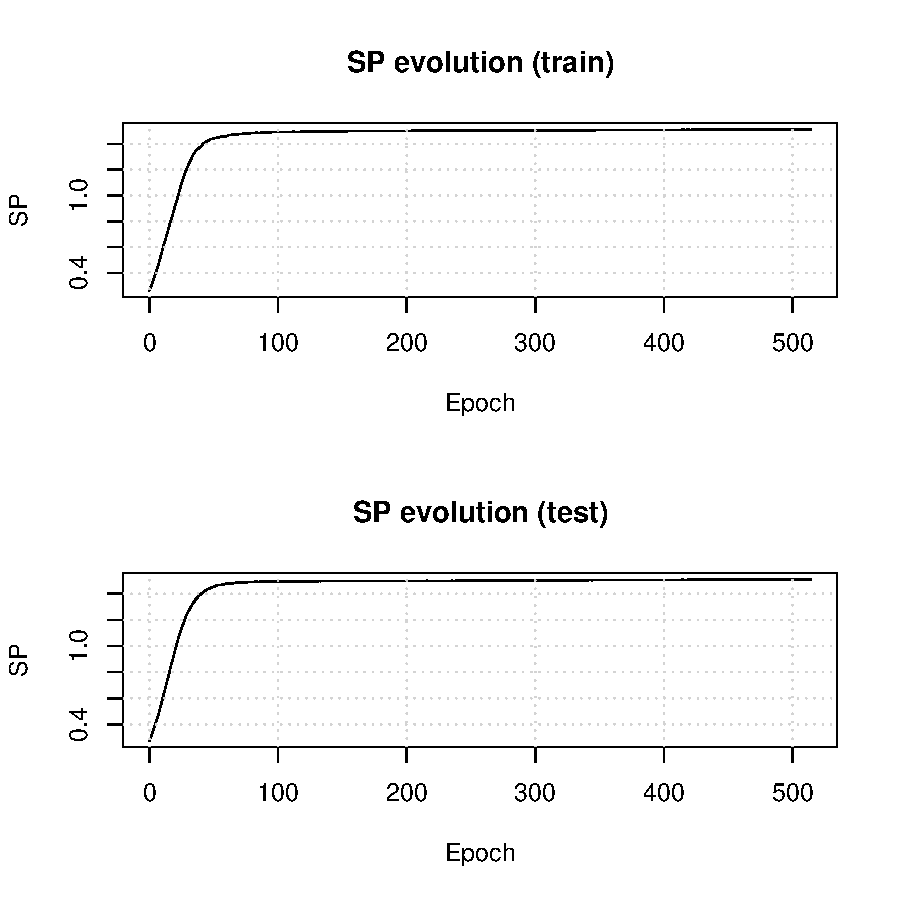
\includegraphics[scale=0.98]{t2calo-mlp/sp-evolution}
\end{center}
\caption{Evolução do produto SP para os conjuntos de treino e teste de um
discriminador elétron/jato neural para as variáveis do T2Calo.}
\label{fig:best-t2calo-mlp-sp}
\end{figure}

O sistema estabiliza após cerca de 300 passos, considerando a evolução do
EMQ. No que tange capacidade discriminante, aferida através do produto SP,
após cerca de 100 passos, o sistema parece se tornar irrelevante à contínua
redução do EMQ. A Figura~\ref{fig:best-t2calo-mlp-output} mostra as saídas da
rede, no final do treinamento, para elétrons (em cima) e jatos (em baixo). A
saída para elétrons é fixada em $-1$ e para jatos, em $+1$. Nota-se que,
diferentemente ao sistema LMS, há uma notável separação entre as classes
proporcionada pelo emprego de um discriminador neural. O ponto ótimo de
separação pode ser mais facilmente determinado, inclusive por inspeção
visual. 

\begin{figure}
\begin{center}
\includegraphics[scale=0.98]{t2calo-mlp/test-output}
\end{center}
\caption{Saída para o conjunto de teste, do discriminador neural baseado nas
características extraídas pelo T2Calo.}
\label{fig:best-t2calo-mlp-output}
\end{figure}

Diferentemente do sistema linear baseado no LMS, uma rede neural poderá traçar
uma superfície curva no espaço de entrada (número de dimensões $=4$),
melhorando a separação entre as classes que se deseja detetar. Esta última
figura mostra o resultado desta capacidade discriminativa. Ainda sim, como é
possível inspecionar na Figura~\ref{fig:best-t2calo-test-roc}, a capacidade
discriminante deste algoritmo neural resta bastante próxima à do sistema
baseado num detetor LMS, chegando, em alguns pontos da R.O.C. a ser inferior.

\begin{figure}
\begin{center}
\includegraphics[scale=0.98]{t2calo-mlp/mlp-vs-lms-vs-egamma-roc}
\end{center}
\caption{R.O.C. para o conjunto de teste, do discriminador neural baseado nas
características extraídas pelo T2Calo, comparado com o detetor baseado no LMS
e a técnica de otimização baseado algoritmo EGammaHypo.}
\label{fig:best-t2calo-test-roc}
\end{figure}

O valor do produto SP máximo na curva para o detetor neural está nas
coordenadas onde a deteção de elétrons é igual a $93,25\%$ e o falso-alarme em
jatos é $88,79\%$ ($\approx 2,80$~kHz de falso-alarme). Estes valores
correspondem a um produto SP de $1,51$, tal qual ao caso do discriminador
LMS. Uma verificação das eficiências parcias por região em $\eta$ e em $\phi$
revelam uma estrutura bastante semelhante aos sistemas de deteção precedentes,
como mostram as Figuras~\ref{fig:best-t2calo-test-sp-eta} e
\ref{fig:best-t2calo-test-sp-phi}. 

\begin{figure}
\begin{center}
\includegraphics[scale=0.98]{t2calo-mlp/test-sp-eta}
\end{center}
\caption{Análise do produto SP ao longo de $\eta$ para o discriminador neural
baseado nas saídas do T2Calo.}
\label{fig:best-t2calo-test-sp-eta}
\end{figure}

\begin{figure}
\begin{center}
\includegraphics[scale=0.98]{t2calo-mlp/test-sp-phi}
\end{center}
\caption{Análise do produto SP ao longo de $\phi$ para o discriminador neural
baseado nas saídas do T2Calo.}
\label{fig:best-t2calo-test-sp-phi}
\end{figure}

A Figura~\ref{fig:best-t2calo-test-sp-emet} mostra o valor relativo do produto
SP for faixa de energia transversa na seção e.m.. Um comparativo entre os 3
métodos do produto SP por faixas de energia descritos até agora se segue
na Figura~\ref{fig:best-t2calo-versus-others-emet}. Os dados nesta figura
correspondem aos do conjunto de teste, para um corte efetuado em $-0.273$ para
o discriminador neural, e para os melhores resultados obtidos com os outros
dois sistemas de deteção de forma equivalente.

\begin{figure}
\begin{center}
\includegraphics[scale=0.98]{t2calo-mlp/test-sp-emet}
\end{center}
\caption{Análise do produto SP ao longo de $E^{e.m.}_T$ para o discriminador
neural baseado nas saídas do T2Calo.}
\label{fig:best-t2calo-test-sp-emet}
\end{figure}

\begin{figure}
\begin{center}
\includegraphics[scale=0.98]{t2calo-mlp/mlp-vs-lms-vs-egamma-et}
\end{center}
\caption{Comparativo do produto SP para os 3 detetores abordados até aqui, por
faixa de energia e.m. transversa.}
\label{fig:best-t2calo-versus-others-emet}
\end{figure}

É possível notar que o sistema neural ganha nas faixas energéticas onde há
mais eventos, porém apresenta uma eficiência marginalmente mais baixa conforme
a energia na seção e.m. aumenta. Num geral, os três sistemas possuem
características bastante próximas nesta análise, concordando entre si. As
análises de relevância, tanto baseadas no EMQ quanto no valor máximo do
produto SP encontram-se nas Figuras~\ref{fig:best-t2calo-mse-relevance} e
\ref{fig:best-t2calo-sp-relevance}. A primeira análise (EMQ) nota-se que há
concordãncia, resguardadas as diferenças nos padrões de saída em cada um dos
casos, na relevância de cada característica neste quesito. O método neural, no
entanto, acentua a falta de importância da componente hadrônica na saída da
rede. Na análise de relevância baseada no máximo do produto SP nota-se que a
ordem de relevância está alterada. Na primeira análise, a variável $\rcore$
parece ser a mais importante, seguindo-se das variáveis $\eratio$, $\ethad$ e
finalmente $\etem$. Baseando-se na variação do produto SP, a variável mais
importante na discriminação é $\eratio$, seguindo-se então de $\rcore$,
$\ethad$ e $\etem$. Diferentemente do sistema linear, as três mais importantes
variáveis de discriminação possuem valores de relevância relativamente
próximos (nos arredores de $0,10$ para $\etem$, $0,15$ para $\rcore$ e $0,20$
para $\eratio$). No sistema linear, a relevância na deteção é fortemente
encabeçada pela variável $\rcore$, com as outras variáveis cerca de uma ordem
de magnitude menos relevantes. 

Um outro ponto observável na análise baseada na variação do produto SP é que,
para o conjunto de treino, a variável $\etem$ possui relevância de
discriminação negativa, encontrando-se aproximadamente em $-0,005$. Este
resultado indica que esta variável estaria atrapalhando o processo de deteção.
Porém, uma vez que seu valor homólogo para o conjunto de teste tenha valor
positivo, nas mesmas proporções, assume-se que este resultado advém,
possivelmente, de uma flutuação estatística e não representa uma real
tendência da variável em questão. Observando os valores de relevância baseados
na diferença do produto SP para os outros 9 testes realizados para o mesmo
conjunto de parâmetros de treinamento, nota-se que esta tendência repete-se em
apenas alguns dos testes, reforçando a conclusão de que este resultado se
trataria apenas de uma flutuação estatística.

\begin{figure}
\begin{center}
\includegraphics[scale=0.98]{t2calo-mlp/relevance-mse}
\end{center}
\caption{Os valores de relevância para os conjunto de treino
(cinza claro) e teste (em cinza escuro), para as 4 variáveis do T2Calo e
considerando-se o classificador neural em estudo.}
\label{fig:best-t2calo-mse-relevance}
\end{figure}

\begin{figure}
\begin{center}
\includegraphics[scale=0.98]{t2calo-mlp/relevance-sp}
\end{center}
\caption{Os valores de relevância de discriminação para os conjunto de treino
(cinza claro) e teste (em cinza escuro), para as 4 variáveis do T2Calo e
considerando-se o classificador neural em estudo.}
\label{fig:best-t2calo-sp-relevance}
\end{figure}

Estas análises também indicam que, tendo por base conjunto de variáveis do
T2Calo, as classes de elétrons e jatos sejam linearmente separáveis. Este
resultado é bastante natural, dado que este conjunto de características tenha
sido otimizado para uma análise baseada em cortes definidos por um operador
experimentado. A Figura~\ref{fig:t2calo-mlp-best-net} mostra uma representação
discriminador neural discutido até agora, para fins ilustrativos. Na próxima
seção definiremos um novo tipo de extração de características que terá por
objetivo maximizar a deteção de elétrons e jatos.

\begin{figure}
\begin{center}
\begin{sideways}
\includegraphics[scale=0.30]{t2calo-mlp/mlp-end}
\end{sideways}
\end{center}
\caption{Diagrama de fluxo do sistema de deteção elétron/jato, neural, usando as
características do T2Calo como entrada.}
\label{fig:t2calo-mlp-best-net}
\end{figure}

\section{Mapeamento topológico}

O algoritmo T2Calo, durante a análise conduzida no LVL2, compacta a informação
da RoI representando um candidato à elétron em quatro quantidades altamente
discrimantes. Tendo estes valores por base obteve-se os seguintes resultados:

\begin{enumerate}
\item Para o EGammaHypo, $91,85\%$ de eficiência na deteção de elétrons contra
$10,19\%$ de falso alarme em jatos;
\item Para detetor LMS, $91,64\%$ para elétrons contra $9,35\%$ de falso alarme;
\item Para uma rede neural, $93,25\%$ para elétrons contra $11,21\%$ de falso
alarme.
\end{enumerate}

Embora as técnicas (LMS e MLP) propostas sejam mais robustas quanto à operação
e manutenção, a qualidade física da separação não é tão afetada. Isto se deve,
principalmente, à agressiva compressão nos dados proporcionada pelo algoritmo
de extração de características. Ainda que não seja viável a deteção de objetos
usando toda a informação da RoI (cerca de 1300 células), é possível encontrar
um método que se situe a meio caminho entre este dois extremos.

Nesta seção, propõe-se um método de compactação da informação da RoI que
utiliza a topologia do evento para gerar um conjunto de características que
pode ser usado para atingir maiores eficiências de deteção de elétrons e
menores valores de falso-alarme.

\subsection{Topologia de uma RoI e anelamento}

Observando-se a interação de elétrons e jatos (enquanto falsos-elétrons) com
os calorímetros, é possível assumir que estes objetos interagirão de forma
aproximadamente isotrópica em relação ao eixo $\eta$ do detetor. Ou seja, dado
um ponto de impacto inicial, a partícula tende a decair em objetos menos
energéticos ao redor do eixo de penetração. Este fenômeno ocorrerá de forma
expansiva, formando finalmente um cone de deposição energética, como o
exemplificado na Figura~\ref{fig:cone}.

\begin{figure}
\begin{center}
\includegraphics{msc/cone}
\end{center}
\caption{Modelo de um objeto e.m. interagindo com um calorímetro.}
\label{fig:cone}
\end{figure}

A Figura~\ref{fig:electron-roi} mostra um gráfico com a deposição energética na
segunda camada e.m. de uma RoI proveniente de um elétron simulado. As partes
acinzentadas indicam deposição energética, enquanto que as partes em branco
indicam que houve pouca ou nenhuma deposição energética na região.

\begin{figure}
\begin{center}
\includegraphics[scale=0.6]{roi-em2}
\end{center}
\caption{Imagem tri-dimensional mostrando o padrão de deposição energética de
um elétron simulado na segunda camada e.m. do calorímetro do ATLAS.}
\label{fig:electron-roi}
\end{figure}

Como colocado na Seção~\ref{sec:e-detection}, a topologia da interação do
objeto em análise com os calorímetros define, com boa margem de sucesso o tipo
do mesmo. Elétrons tendem a um menor espalhamento que jatos, percorrendo
menores distâncias ao longo do eixo $\eta$. Por outro lado, jatos tendem a
radializar a deposição energética, formando cones mais largos e possivelmente
mais profundos.

Levando-se em consideração a formatação dos calorímetros do ATLAS e sua
granularidade, sugere-se o seguinte algoritmo de compactação:

\begin{description}
\item[\ding{182}] Define-se, para cada camada, o centro de posição
energética. Isto é feito de forma simplificada, procurando para todas as
células dentro de uma mesma camada, aquela célula com maior deposição
energética;
\item[\ding{183}] Uma vez que o centro de interação esteja definido, formar um
conjunto de anéis com formato retangular que circumdem este pico. A largura
destes anéis é ajustada de forma que a largura do anel de energia seja a mesma
que de uma célula dentro da camada estudada;
\item[\ding{184}] Para cada anel, somar os valores energéticos das células que
recaem sobre o seu interior.
\end{description}

A Figura~\ref{fig:rings} esquematiza tal algoritmo. Nesta figura encontram-se
exemplos de anéis de energia formados em 4 diferentes camadas dos calorímetros
do detetor ATLAS. Próximo ao centro da RoI, nota-se uma célula que destaca,
hipoteticamente, o centro de deposição energética que a etapa \ding{182} do
algoritmo encontraria. Em seguida, as células de cada segmento são somadas
para a obtenção das ``características'' do objeto a ser discriminado.

\begin{figure}
\begin{center}
\includegraphics[scale=0.5]{msc/rings}
\end{center}
\caption{Esquematização do processo de anelamento para as diferentes camadas
dos calorímetros do ATLAS.}
\label{fig:rings}
\end{figure}

A granularidade dos anéis respeita a granularidade \emph{típica} das células
na camada. Sabe-se, no entanto, que a granularidade das células varia com
$\eta$ no detetor. Nos casos onde a granularidade é diferente da granularidade
padrão na camada, atribuir-se-á a energia da célula ao anel onde recai o
centro da mesma. Este algoritmo também é resiliente à dados
faltantes\footnote{Ocorrendo, potencialmente, com a falha de um canal de
leitura ou do sistema de aquisição de dados.}, uma vez que células que não
puderem ser lidas apenas não serão contabilizadas. Isto evita procedimentos de
verificação especiais que poderiam comprometer o desempenho do algoritmo de
compactação proposto. Através desta figura observa-se igualmente que algumas
camadas, devido ao formato não simétrico das células (maiores numa direção que
na outra), terão anéis abertos ou incompletos. Desta forma, marcou-se
segmentos que pertencem ao mesmo anel com um número indicando a que anel
determinado segmento pertence.

Um problema recorrente nos algoritmos de filtragem do ATLAS é a região de
\eng{wrap-around} da variável $\phi$, já que o detetor tem formato
cilíndrico. Um cuidado especial deve ser tomado na confecção dos anéis,
levando-se em consideração que, por exemplo, a região com $\phi = 6,18$ está
bastante próxima a região com $\phi = 0,1$, apesar da diferença
numérica. Outro problema encontrado é que diferentes partes do sistema de
localização dos dados dentro do Athena identificam a região do detetor onde
$\phi > \pi$ de maneiras distintas. Para parte do código (relativa à seção
e.m.), o detetor se encontra na área entre $[-\pi, \pi]$ enquanto que para
outra (parte hadrônica), o detetor se encontra na área entre $[0, 2\pi]$. Para
resolver este problema, implementou-se um algoritmo que normaliza as
diferenças em ambos os casos.

Ademais, por se tratar de elétrons ou jatos na qualidade de falsos-elétrons, é
bastante provável que a relação sinal-ruído seja pequena nas camadas traseiras
do detetor, principalmente na região hadrônica. A Figura~\ref{fig:roi-had-9}
mostra a deposição energética de um elétron na primeira camada do detetor
hardrônico. Nesta figura este fenômeno pode ser bem observado.

\begin{figure}
\begin{center}
\includegraphics[scale=0.6]{roi-had-9}
\end{center}
\caption{Imagem tri-dimensional mostrando o padrão de deposição energética de
um elétron simulado na primeria camada hadrônica do calorímetro do ATLAS.}
\label{fig:roi-had-9}
\end{figure}

Para evitar que o ruído inerente à eletrônica do detetor possa interferir com
o aferimento do centro de deposição energética, a procura do pico em uma
camada está restrita a uma região de $\eta=0,1\times\phi=0,1$ ao redor do pico
de deposição na segunda camada e.m.. Como já colocado um capítulo anterior
deste trabalho, a segunda camada e.m. é a mais profunda do sistema de
calorimetria, concentrando a maior parte da energia dos elétrons que interagem
com este detetor. Desta forma, se há um pico de deposição energética, este é
considerado para a formação dos anéis. De outra maneira, um ponto aleatório
(aquele com maior energia) dentro da sub-janela definida pelo pico de
deposição energética na segunda camada e.m. é escolhido.

Tomando-se em consideração a granularidade padrão de todas as camadas do
calorímetro (7 no total, incluindo o pré-irradiador), a configuração sugerida
para o número de anéis pode ser encontrada na Tabela~\ref{tab:ring-config}. O
número de anéis em cada camada leva em consideração o número máximo de anéis
que podem ser formados considerando-se uma sub-região de $0,4 \times 0,4$ no
plano $\eta\times\phi$. É interessante notar que nem sempre esta região
cobrirá completamente uma região do mesmo tamanho, já que o posicionamento dos
anéis depende do centro de deposição energética em cada camada. No entanto,
como podemos ver no exemplo do T2Calo, uma região de $0,3 \times 0,3$ está
garantida ao redor do pico de energia, o que é suficiente para a análise de
elétrons \cite{daqnote00-02}.

\begin{table}
\begin{center}
\begin{tabular}{>{\bfseries}l r r r}
Camada & Número de Anéis & Larg. do anel ($\eta$) & Larg. do anel ($\phi$) \\ \hline
Pré-irradiador & 8 & $0,025$ & $\frac{\pi}{32} \approx 0,098174$ \\ 
1\eira\ e.m. & 64 & $0,0031245$ & $\frac{\pi}{32} \approx 0,098174$ \\ 
2\eira\ e.m. & 8 & $0,025$ & $\frac{\pi}{128} \approx 0,024544$ \\ 
3\eira\ e.m. & 8 & $0,05$ & $\frac{\pi}{128} \approx 0,024544$ \\ 
1\eira\ hadrônica & 4 & $0,1$ & $\frac{\pi}{32} \approx 0,098174$ \\ 
2\eira\ hadrônica & 4 & $0,1$ & $\frac{\pi}{32} \approx 0,098174$ \\ 
3\eira\ hadrônica & 4 & $0,1$ & $\frac{\pi}{32} \approx 0,098174$ \\ \hline
Total & 100 & & \\ \hline
\end{tabular}
\end{center}
\caption{Configuração para os anéis formados à partir de uma RoI de tamanho
$\eta = 0,4 \times \phi = 0,4$.}
\label{tab:ring-config}
\end{table}

Um total de $100$ anéis forma o conjunto de entrada para o novo sistema de
discriminação elétron/jato. Nota-se que o primeiro anel de cada conjunto será
considerado o pico de deposição energética na camada. Para classificar os
padrões neste espaço de alta dimensionalidade, utilizaremos detetores baseados
em redes neurais tipo MLP como descrito nas seções anteriores.

\subsubsection{Normalização}

Uma vez que estaremos lidando com os diferenciais energéticos dentro da mesma
camada, por muitas vezes sutis, faz-se necessário que a normalização aplicada
aos conjuntos de anéis seja compatível com a deteção destas
diferenças. Ademais, outros estudos \cite{seixas:pca} já demonstraram que a
informação periférica dentro de cada camada de uma RoI é tão ou mais
importante à discriminação que a quantidade de energia depositada no pico. Por
estas razões, neste trabalho propomos um sistema de normalização dos dados da
RoI baseado em um conjunto de razões cujo o denominador diminui, de forma
relacionada a energia na camada, do centro para as bordas da região de
interesse. Desta forma, o pico de deposição energética na camada (ou
``primeiro anel'') teria um fator de normalização maior que o segundo anel,
que seria por sua vez maior que o fator de normalização aplicado ao terceiro
anel e, assim, sucessivamente. O algoritmo está descrito matematicamente na
Tabela~\ref{tab:seq}.

\begin{table}
\renewcommand{\baselinestretch}{1}
\begin{center}
\begin{tabular}{>{\bfseries}l r r}
Anel & Normalização & Soma em anel \\ \hline
1 & $E$ (total da camada) & $E_1$\\
2 & $E - E_1$ & $E_2$ \\
3 & $E - E_1 - E_2$ & $E_3$\\
4 & $E - E_1 - E_2 - E_3$ & $E_4$\\
\dots  & \dots \\
N-4 & $E - E_1 - E_2 - ... - E_{N-5}$ & $E_{N-4}$ \\
N-3 & $E - E_1 - E_2 - ... - E_{N-5} - E_{N-4}$ & $E_{N-3}$ \\
N-2 & $E - E_1 - E_2 - ... - E_{N-5} - E_{N-4}$ & $E_{N-2}$ \\
N-1 & $E - E_1 - E_2 - ... - E_{N-5} - E_{N-4}$ & $E_{N-1}$ \\
N & $E - E_1 - E_2 - ... - E_{N-5} - E_{N-4}$ & $E_N$ \\
\end{tabular}
\end{center}
\renewcommand{\baselinestretch}{1.5}
\caption{Algoritmo para a ``Normalização Seqüencial''.}
\label{tab:seq}
\end{table}

Neste algoritmo, o primeiro anel (pico de deposição energética) será
normalizado pelo valor da energia total na camada. O segundo anel pelo valor
da camada subtraindo-se o valor de deposição energética no primeiro anel. O
terceiro anel, pelo valor da energia na camada menos o valor do primeiro e
segundo aneís e desta forma, recursivamente até que todos os anéis estejam
normalizados. Nos referiremos à este algoritmo à partir de agora como
algoritmo de ``Normalização Seqüencial''.

Nota-se que este tipo de normalização poderá amplificar em demasiado os
valores periféricos. Isto é desejável para os anéis que se sucedem ao pico de
energia na camada, porém nem tanto para os anéis da periferia da RoI, onde a
relação sinal-ruído é praticamente nula. Desta forma, propõe-se que, à partir
de um determinado limiar de energia, o fator de normalização torne-se
constante. Desta forma evita-se que o sinal ruidoso das bordas influencie o
sistema de discriminação de maneira significativa.

O sub-pacote \texttt{rbuild} do \eng{NeuralRinger} contém a implementação de
referência para este processo de anelamento descrito. Ademais, este pacote
pode ser re-configurado de forma a definir a largura dos aneis de cada camada
ou o número máximo de anéis por camada. Assim, o sistema de anelamento torna-se
independente do tamanho real da RoI e, portanto, independente de quão completo
são os dados recebidos pelo processador do LVL2. Anéis sem dados recebem o
valor \eng{default} que é igual a zero. O formato do arquivo de configuração é
também em XML, o que simplifica a leitura e escrita dentro do contexto do
projeto.

\subsubsection{Dados}

Os dados utilizados nas seções anteriores não podem ser re-utilizados para
esta porção do projeto, uma vez que é necessita-se do acesso aos dados
``brutos'' da RoI. Em outras palavras, deseja-se acesso aos mesmos dados
utilizados pelo T2Calo para a operação de extração de características que este
algoritmo realiza. De posse destes dados, é possível definir a operação de
compactção topológica proposta. A Figura~\ref{fig:datagen} mostra o sistema
que foi utilizado para a obtenção dos dados. Para cada RoI que é analisada
pelo T2Cal, um conjunto de células é carregado dos arquivos de dados
iniciais. Em seguida, os valores das células são calibrados e mapeados na
geometria do detetor de forma que possam ser mais facilmente acessados pelo
algoritmo de extração de características. À partir deste ponto, o T2Calo tem
acesso aos dados e, é exatamente neste ponto que inserimos um \eng{patch}, que
permite que os valores das células ``vistas'' pelo algoritmo sejam guardadas
em um arquivo separado.

\begin{figure}
\begin{center}
\includegraphics[scale=0.74]{datagen}
\end{center}
\caption{Estratégia para obter acesso aos dados tais quais processados pelo
algoritmo T2Calo.}
\label{fig:datagen}
\end{figure}

O formato deste arquivo é legível pelo sub-pacote \texttt{roiformat} do
\eng{NeuralRinger} e pode ser transformado em uma base de dados de anéis
utilizando-se o programa \texttt{ringer}, descrito no
Apêndice~\ref{ap:framework}. Desta forma, criou-se uma base de dados à partir
do mesmo conjunto de eventos analisados na caracterização do desempenho físico
do T2Calo. Esta nova base de dados tem cerca de $30000$ eventos com a mesma
proveniência e características dos eventos analisados até o momento.

\subsection{Discriminação baseada em anelamento}

O processo de anelamento reduz o espaço de dados de entrada em uma RoI (cerca
de 1300 células) para 100 valores correspondes aos anéis formados com os dados
das 7 camadas dos calorímetros. Sería difícil conceber um sistema de
discriminação simples como o proposto para o EGammaHypo neste caso, uma vez
que a possibilidade de combinações é muito grande. Neste caso, adota-se um
sistema de discriminação neural, conectado à saída do sistema de anelamento
que executará o processo de deteção.

Tal qual nos sistemas anteriores, executou-se uma rápida análise do espaço dos
parâmetros de treinamento neural. A Tabela~\ref{tab:ringer-param-optimization}
resume os resultados e indica os valores de taxa de treinamento, tamanho da
época e número de neurônios escondidos utilizados. Para cada tripla destes
parâmetros, 5 testes foram executados e o resultado exposto na tabela
representa a média e desvio padrões levando-se em consideração estas 5
instâncias.

\begin{table}
\begin{center}
\renewcommand{\baselinestretch}{1.0}
{\tiny
\begin{tabular}{|l|l|l|r|r|r|} \hline
\rottext{Tx. de Aprendizado} & \rottext{Tamanho da Época} & \rottext{Neurônios escondidos} & \rottext{Número de iterações} & \rottext{Produto SP (treino)} & \rottext{Produto SP (teste)} \\ \hline \hline

0.0100 & 100 & 4 & $356\pm78$ & $1.6329\pm0.0149$ & $1.6199\pm0.0156$ \\ \hline
0.0100 & 100 & 6 & $372\pm88$ & $1.6237\pm0.0247$ & $1.6202\pm0.0183$ \\ \hline
0.0100 & 100 & 8 & $280\pm39$ & $1.5987\pm0.0210$ & $1.6017\pm0.0215$ \\ \hline
0.0100 & 100 & 10 & $337\pm58$ & $1.6263\pm0.0385$ & $1.6137\pm0.0320$ \\ \hline
0.0100 & 200 & 4 & $366\pm43$ & $1.6119\pm0.0335$ & $1.5986\pm0.0302$ \\ \hline
0.0100 & 200 & 6 & $299\pm33$ & $1.5961\pm0.0236$ & $1.5945\pm0.0264$ \\ \hline
0.0100 & 200 & 8 & $340\pm62$ & $1.6246\pm0.0250$ & $1.6144\pm0.0221$ \\ \hline
0.0100 & 200 & 10 & $287\pm75$ & $1.5994\pm0.0444$ & $1.5968\pm0.0342$ \\ \hline
0.0100 & 500 & 4 & $285\pm64$ & $1.5914\pm0.0211$ & $1.5880\pm0.0225$ \\ \hline
0.0100 & 500 & 6 & $296\pm53$ & $1.6061\pm0.0251$ & $1.5998\pm0.0200$ \\ \hline
0.0100 & 500 & 8 & $254\pm56$ & $1.5981\pm0.0165$ & $1.5937\pm0.0156$ \\ \hline
0.0100 & 500 & 10 & $343\pm68$ & $1.6177\pm0.0273$ & $1.6120\pm0.0225$ \\ \hline
0.0100 & 1000 & 4 & $250\pm44$ & $1.5974\pm0.0215$ & $1.5897\pm0.0183$ \\ \hline
0.0100 & 1000 & 6 & $260\pm24$ & $1.5999\pm0.0307$ & $1.5998\pm0.0201$ \\ \hline
0.0100 & 1000 & 8 & $267\pm41$ & $1.6024\pm0.0175$ & $1.5934\pm0.0193$ \\ \hline
0.0100 & 1000 & 10 & $271\pm46$ & $1.5876\pm0.0182$ & $1.5863\pm0.0164$ \\ \hline

0.0200 & 100 & 4 & $460\pm106$ & $1.7245\pm0.0227$ & $1.6928\pm0.0200$ \\ \hline
0.0200 & 100 & 6 & $347\pm57$ & $1.7056\pm0.0141$ & $1.6774\pm0.0176$ \\ \hline
0.0200 & 100 & 8 & $421\pm78$ & $1.7215\pm0.0163$ & $1.6920\pm0.0149$ \\ \hline
0.0200 & 100 & 10 & $366\pm80$ & $1.7120\pm0.0208$ & $1.6888\pm0.0179$ \\ \hline
0.0200 & 200 & 4 & $265\pm67$ & $1.6716\pm0.0333$ & $1.6549\pm0.0265$ \\ \hline
0.0200 & 200 & 6 & $315\pm72$ & $1.6893\pm0.0192$ & $1.6688\pm0.0147$ \\ \hline
0.0200 & 200 & 8 & $283\pm57$ & $1.6870\pm0.0154$ & $1.6627\pm0.0156$ \\ \hline
0.0200 & 200 & 10 & $301\pm58$ & $1.6903\pm0.0268$ & $1.6662\pm0.0197$ \\ \hline
0.0200 & 500 & 4 & $351\pm42$ & $1.7028\pm0.0094$ & $1.6774\pm0.0098$ \\ \hline
0.0200 & 500 & 6 & $348\pm61$ & $1.6941\pm0.0202$ & $1.6688\pm0.0125$ \\ \hline
0.0200 & 500 & 8 & $298\pm69$ & $1.6793\pm0.0194$ & $1.6570\pm0.0216$ \\ \hline
0.0200 & 500 & 10 & $260\pm23$ & $1.6789\pm0.0076$ & $1.6551\pm0.0041$ \\ \hline
0.0200 & 1000 & 4 & $226\pm58$ & $1.6568\pm0.0287$ & $1.6468\pm0.0176$ \\ \hline
0.0200 & 1000 & 6 & $280\pm68$ & $1.6850\pm0.0162$ & $1.6672\pm0.0144$ \\ \hline
0.0200 & 1000 & 8 & $281\pm65$ & $1.6955\pm0.0212$ & $1.6700\pm0.0194$ \\ \hline
0.0200 & 1000 & 10 & $263\pm47$ & $1.6812\pm0.0218$ & $1.6632\pm0.0214$ \\ \hline

0.0500 & 100 & 4 & $3416\pm655$ & $1.8302\pm0.0144$ & $1.7872\pm0.0091$ \\ \hline
0.0500 & 100 & 6 & $2173\pm1092$ & $1.8095\pm0.0192$ & $1.7755\pm0.0121$ \\ \hline
0.0500 & 100 & 8 & $2263\pm1887$ & $1.8103\pm0.0308$ & $1.7727\pm0.0215$ \\ \hline
0.0500 & 100 & 10 & $2284\pm1657$ & $1.8143\pm0.0278$ & $1.7784\pm0.0166$ \\ \hline
0.0500 & 200 & 4 & $1283\pm324$ & $1.7947\pm0.0028$ & $1.7668\pm0.0036$ \\ \hline
0.0500 & 200 & 6 & $760\pm601$ & $1.7773\pm0.0202$ & $1.7478\pm0.0197$ \\ \hline
0.0500 & 200 & 8 & $705\pm712$ & $1.7730\pm0.0176$ & $1.7473\pm0.0166$ \\ \hline
0.0500 & 200 & 10 & $520\pm273$ & $1.7741\pm0.0155$ & $1.7455\pm0.0154$ \\ \hline
0.0500 & 500 & 4 & $532\pm321$ & $1.7731\pm0.0167$ & $1.7431\pm0.0167$ \\ \hline
0.0500 & 500 & 6 & $382\pm95$ & $1.7654\pm0.0114$ & $1.7386\pm0.0138$ \\ \hline
0.0500 & 500 & 8 & $291\pm74$ & $1.7577\pm0.0101$ & $1.7292\pm0.0136$ \\ \hline
0.0500 & 500 & 10 & $291\pm54$ & $1.7572\pm0.0095$ & $1.7284\pm0.0105$ \\ \hline
0.0500 & 1000 & 4 & $277\pm45$ & $1.7542\pm0.0071$ & $1.7284\pm0.0094$ \\ \hline
0.0500 & 1000 & 6 & $248\pm52$ & $1.7497\pm0.0065$ & $1.7191\pm0.0135$ \\ \hline
0.0500 & 1000 & 8 & $244\pm50$ & $1.7464\pm0.0132$ & $1.7197\pm0.0142$ \\ \hline
0.0500 & 1000 & 10 & $250\pm48$ & $1.7460\pm0.0194$ & $1.7220\pm0.0166$ \\ \hline

0.1000 & 100 & 4 & $4962\pm82$ & $1.8549\pm0.0102$ & $1.7948\pm0.0065$ \\ \hline
0.1000 & 100 & 6 & $4951\pm63$ & $1.8767\pm0.0093$ & $1.8018\pm0.0059$ \\ \hline
\textbf{0.1000} & \textbf{100} & \textbf{8} & \textbf{$4892\pm99$} & \textbf{$1.8852\pm0.0088$} & \textbf{$1.8070\pm0.0048$} \\ \hline
0.1000 & 100 & 10 & $4972\pm27$ & $1.8841\pm0.0120$ & $1.8042\pm0.0054$ \\ \hline

% missing tests with epoch size = 200

0.1000 & 500 & 4 & $2866\pm1435$ & $1.8466\pm0.0285$ & $1.7884\pm0.0143$ \\ \hline
0.1000 & 500 & 6 & $2089\pm421$ & $1.8416\pm0.0133$ & $1.7908\pm0.0057$ \\ \hline
0.1000 & 500 & 8 & $1286\pm868$ & $1.8160\pm0.0322$ & $1.7770\pm0.0156$ \\ \hline
0.1000 & 500 & 10 & $1296\pm652$ & $1.8156\pm0.0316$ & $1.7705\pm0.0204$ \\ \hline
0.1000 & 1000 & 4 & $738\pm607$ & $1.7988\pm0.0283$ & $1.7624\pm0.0205$ \\ \hline
0.1000 & 1000 & 6 & $977\pm408$ & $1.8098\pm0.0139$ & $1.7757\pm0.0080$ \\ \hline
0.1000 & 1000 & 8 & $815\pm285$ & $1.8010\pm0.0078$ & $1.7706\pm0.0034$ \\ \hline
0.1000 & 1000 & 10 & $272\pm116$ & $1.7778\pm0.0160$ & $1.7498\pm0.0148$ \\ \hline

\end{tabular}}
\renewcommand{\baselinestretch}{1.0}
\end{center}
\caption{Análise dos parâmetros de treinamento para um detetor neural cuja a
entrada são os 100 anéis resultantes do processamento de uma RoI.}
\label{tab:ringer-param-optimization}
\end{table}

Os testes realizados sugerem que uma combinação entre a taxa de treinamento
igual à $0,01$, o tamanho da época de treinamento igual à $100$ e o número de
neurônios escondidos igual à $8$ maximizem o potencial discriminante do
sistema, que já se apresenta superior aos testes usando as características do
T2Calo. Uma análise da tabela indica que a utilização de taxas de treinamento
muito pequenas, para este sistema, é prejudicial. Isto pode ocorrer seja
quando a superfície de erro não possui uma inclinação relativamente acentuada
que faça o sistema convergir de forma suficiente rápida, seja pela existência
de mínimos locais, ou ainda, uma combinação destas duas
características. Realizou-se, igualmente, testes com taxas de aprendizado
maior que $0,01$. Estes testes demonstraram grande instabilidade na fase de
treinamento e foram descartados como possibilidade para o sistema final.

O número de neurônios escondidos ideal aparenta estar entre 8 e 10. Os testes
indicam que exista pouca diferença estatítisca entre as duas opções e portanto
escolhe-se 8. Esta escolha se traduz em um sistema de deteção menos complexo,
o que é positivo em geral. O tamanho ideal da época de treinamento, ou
batelada parece ter uma correlação bastante forte com a qualidade do
discriminador final. Quanto maior a época, menor a eficiência do detetor, em
média, tendo-se por vista os valores de produto SP destacados. Mais uma vez,
realizou-se testes com valores para o tamanho da época menores que 100. Estes
testes demonstraram maior instabilidade no treinamento sem que houvesse um
aumento no valor médio do produto SP para o conjunto de testes. Desta forma,
concluiu-se que os valores escolhidos da
Tabela~\ref{tab:ringer-param-optimization} representem um bom compromisso 
dentre os parâmetros de treinamento que se deseja otimizar para este detetor.

\subsubsection{Resultados para o \eng{NeuralRinger}}

Baseando-se nos parâmetros destacados acima, treinou-se dez redes que tiveram
seus pesos sinápticos iniciais fixados em valores aleatórios e diferentes para
cada uma destas iterações. A Figura~\ref{fig:ringer-mlp-mse} mostra a evolução
do EMQ de uma destas redes. A Figura~\ref{fig:ringer-mlp-sp} mostra um gráfico
equivalente para a evolução do produto SP ao longo do treinamento da
rede. Como é possível distinguir, após cerca de 3000 passos de treinamento,
apesar do EMQ continuar a apresentar declínio, a capacidade discriminante da
rede parece pouco influenciada. A capacidade discriminante no que tange o
conjunto de treinamento, apesar da constatação de estagnação do conjunto de
teste, ainda continua a aumentar após os 3000 passos. É interessante observar,
no entanto, que a capacidade discriminante da rede, para o conjunto de teste,
resta inalterada não indicando a ocorrência do fenômeno de
\eng{overtraining}. O mesmo comportamento pode ser observado com a evolução do
EMQ.

\begin{figure}
\begin{center}
\includegraphics[scale=0.98]{ringer-mlp/mse-evolution}
\end{center}
\caption{Evolução do EMQ para os conjuntos de treino e teste de um
discriminador elétron/jato neural para as variáveis do anelador.}
\label{fig:ringer-mlp-mse}
\end{figure}

\begin{figure}
\begin{center}
\includegraphics[scale=0.98]{ringer-mlp/sp-evolution}
\end{center}
\caption{Evolução do produto SP para os conjuntos de treino e teste de um
discriminador elétron/jato neural para as variáveis do anelador.}
\label{fig:ringer-mlp-sp}
\end{figure}

A Figura~\ref{fig:ringer-mlp-output} contém a saída da rede após o treinamento
do detetor neural. Diferentemente aos casos anteriores, o sistema parece
identificar com bastante precisão elétrons e jatos. Um corte em $+0,0302$
estabele o máximo do produto SP (conjunto de teste) para esta rede, com uma
eficiência de $96,55$\% na deteção de elétrons contra apenas $3,12$\% de
falso-alarme em jatos. O produto SP para estes valores é $\approx 1,81$,
representando o melhor valor para este índice obtido até o momento. Este valor
está $0,3$ pontos acima do valor obtido para as saídas do T2Calo usando um
detetor neural ou baseado no algoritmo LMS!

\begin{figure}
\begin{center}
\includegraphics[scale=0.98]{ringer-mlp/test-output}
\end{center}
\caption{Saída para o conjunto de teste, do discriminador neural baseado nas
características extraídas pelo anelador.}
\label{fig:ringer-mlp-output}
\end{figure}

A Figura~\ref{fig:ringer-test-roc} contém um comparativo das R.O.C. entre
todos métodos estudados até o momento. Como é possível perceber, o método
proposto de anelamento, associado a um detetor neural produz um resultado
significativamente melhor para a massa de dados avaliada. Para um mesmo valor
de eficiência na deteção de elétrons, por exemplo $90$\%, o sistema baseado no
anelador aprovará apenas cerca de 400~Hz em jatos ao passo que o sistema
baseado na solução atual (EGammaHypo) para o LVL2, cerca de 2,4~kHz. Por outro
ângulo este resultado traz que, para uma mesma capacidade de aprovar elétrons,
um sistema baseado no anelamento e redes neurais poupará 6 vezes mais o
terceiro nível de filtragem do experimento ATLAS. Se, por outro lado deseja-se
aumentar a eficiência na deteção de elétrons, o anelador consegue, até cerca
de $97$\% de eficiência, manter uma taxa de falso-alarme igual ou inferior a
1~kHz. Para o sistema atual baseado no EGammaHypo, para uma eficiência na
deteção de elétrons de $97$\%, $100$\% dos jatos deveria ser aprovados, o que
seria inviável.

\begin{figure}
\begin{center}
\includegraphics[scale=0.98]{ringer-mlp/mlp-vs-lms-vs-egamma-roc}
\end{center}
\caption{R.O.C. para o conjunto de teste, do discriminador neural baseado nas
características extraídas pelo anelador, comparado com os resultados obtidos
para o T2Calo.}
\label{fig:ringer-test-roc}
\end{figure}

As Figuras~\ref{fig:ringer-test-sp-eta} e \ref{fig:ringer-test-sp-phi} mostram
os valores do produto SP por intervalo em $\eta$ e em $\phi$,
respectivamente. Observa-se, tal qual como nos sistemas anteriores, que a
eficiência de deteção é menor próxima à região do \eng{crack}, no entanto,
maior que nos outros casos. Na parte central do detetor, onde maior parte dos
eventos de interesse se concentrarão, o valor do produto SP é bastante alto,
chegando, em alguns pontos, a aproximar-se de $2,0$. O gráfico equivalente em
$\phi$ mostra a homogenidade esperada.

\begin{figure}
\begin{center}
\includegraphics[scale=0.98]{ringer-mlp/test-sp-eta}
\end{center}
\caption{Análise do produto SP ao longo de $\eta$ para o discriminador neural
baseado nas saídas do anelador.}
\label{fig:ringer-test-sp-eta}
\end{figure}

\begin{figure}
\begin{center}
\includegraphics[scale=0.98]{ringer-mlp/test-sp-phi}
\end{center}
\caption{Análise do produto SP ao longo de $\phi$ para o discriminador neural
baseado nas saídas do anelador.}
\label{fig:ringer-test-sp-phi}
\end{figure}

A Figura~\ref{fig:ringer-test-sp-emet} contém uma análise do produto SP por
intervalo em $\etem$. A eficiência de deteção neste caso apresenta-se
constante, ou aproximadamente constante, até a faixa de energia em torno de
100~GeV, caido abruptamente. Os número no topo de cada barra indicam a
quantidade de RoI's analisadas no intervalo e servem como uma medida da
significância do resultado. Para valores de energia acima de $\approx
100$~GeV, o número de eventos disponíveis para treino e análise cai
significativamente, devido à natureza dos eventos estudados. Por esta razão,
acredita-se que os resultados para altos valores energéticos devam ser
interpretados com maior cuidado.

\begin{figure}
\begin{center}
\includegraphics[scale=0.98]{ringer-mlp/test-sp-emet}
\end{center}
\caption{Análise do produto SP ao longo de $E^{e.m.}_T$ para o discriminador
neural baseado nas saídas do anelador.}
\label{fig:ringer-test-sp-emet}
\end{figure}

As Figuras~\ref{fig:ringer-mse-relevance} e \ref{fig:ringer-sp-relevance}
trazem as análises de relevância para o conjunto de teste, das 100 variáveis
do anelador, tendo em vista a variação do EMQ e do produto SP
respectivamente. Os dois gráficos parecem indicar, igualmente, uma grande
importância nos primeiros anéis de cada camada (veja
Tabela~\ref{tab:ringer-position}). A importância de cada anel diminui com o
afastamento do centro, onde pressupõe-se que a relação sinal ruído seja
inferior. A importância relativa entre os anéis mais importantes e aqueles de
menor importância parece ser menor da perspectiva da relevância de baseada no
produto SP que da relevância clássica. Outra informação que pode ser aferida é
sobre a importância da informação na primeira camada e.m.. Para a relevância
clássica, as variáveis desta camada constituem uma informação essencial na
determinação da saída, estando ao menos uma ordem de magnitude acima da
relevância dos dados de outras camadas. Na avaliação baseada na capacidade
discriminante do sistema, a parte hadrônica é a mais importante. A importância
relativa entre os dados da primeira e segunda camadas e.m. e da primeira
camada hadrônica também difere. Na análise da relevância utilizando a
discriminação, estas três camadas parecem exercer um papel igualmente
importante na deteção de elétrons e jatos.

\begin{figure}
\begin{center}
\includegraphics[scale=0.98]{ringer-mlp/test-mse-relevance}
\end{center}
\caption{Os valores de relevância para os conjunto de teste, para as 100
variáveis do anelador e considerando-se o classificador neural em estudo.}
\label{fig:ringer-mse-relevance}
\end{figure}

\begin{figure}
\begin{center}
\includegraphics[scale=0.98]{ringer-mlp/test-sp-relevance}
\end{center}
\caption{Os valores de relevância de discriminação para os conjunto de teste,
para as 100 variáveis do anelador e considerando-se o classificador neural em
estudo.}
\label{fig:ringer-sp-relevance}
\end{figure}

\begin{table}
\begin{center}
\begin{tabular}{|l|r|r|r|} \hline
\textbf{Camada} & \textbf{Número de anéis} & \textbf{Primeiro} &
\textbf{Último} \\ \hline
Pré-irradiador & 8 & 1 & 8 \\
1\eira e.m. & 64 & 9 & 72 \\
2\eira e.m. & 8 & 73 & 80 \\
3\eira e.m. & 8 & 81 & 88 \\
1\eira hadrônica & 4 & 89 & 92 \\
2\eira hadrônica & 4 & 93 & 96 \\
3\eira hadrônica & 4 & 97 & 100 \\ \hline
\end{tabular}
\end{center}
\caption{Posicionamento relativo dos anéis produzidos pelo anelador no vetor
de entrada ao sistema de deteção neural.}
\label{tab:ringer-position}
\end{table}

\subsection{Compressão baseada na relevância}

A informação de relevância estudada até aqui pode ser aproveitada para que
aplique-se sobre as entradas do discriminador neural, uma poda baseada na
capacidade discriminante de uma variável. Esta poda pode ser feita
automaticamente \cite{andre-enfpc2000} em muitos casos, ou manualmente se
existirem restrições no processo de poda.

De fato, a técnica de normalização seqüêncial dos anéis que é proposta nesta
seção assume a disponbilidade da energia total camada a camada para o cálculo
do fator de normalização para cada anel. Ademais, para calcular o fator de
normalização para o anel $N+1$ em uma mesma camada, necessita-se do valor de
energia do anel $N$. Portanto, se deseja-se manter o anel $N+1$ de uma camada,
é necessário que se mantenha o anel $N$, ao menos para o cálculo do fator de
normalização. De fato, como veremos mais a frente, esta última sugestão seria
uma prática que recompensaria em pouco, visto que a maior parte do tempo de
processamento não está na discriminação neural e sim na aquisição dos
dados. Por outro lado, seria possível considerar que uma poda sempre seria
positiva no que tange a complexidade do discriminador neural que segue o
sistema de anelamento. Ao retirar uma variável da entrada, ao menos 8 conexões
sinápticas do detetor final seriam removidas simultaneamente, levando-se em
consideração a configuração exemplificada anteriormente. 

Observando-se mais uma vez o gráfico da Figura~\ref{fig:ringer-sp-relevance},
podemos concluir que o grau de importância dos anéis diminui, num geral, do
pico de deposição energética ($N = 0$) para as bordas da RoI. Desta forma o
problema da otimização deste sistema, numa primeira aproximação, poderia se
resumir à poda de elementos da periferia, de acordo com a relevância de
discriminação observada naquele gráfico.

Outra técnica que empregaremos será a combinação de camadas menos relevantes,
reduzindo o número de entradas do processador neural, sem que se perca,
necessariamente, a informação de energia presente nos anéis removidos. Uma
outra forma de manter a informação de energia, mas compactando ainda mais a
entrada seria a utilização de anéis cuja a largura dependesse da relevância
dos dados naquela região. Este estudo, reservaremos a um outro projeto. Tendo
em vista a discussão nos parâgrafos anteriores, propõe-se a seguinte variante
do processo de anelamento, baseando-se na relevância de discriminação da
Figura~\ref{fig:ringer-sp-relevance}

\begin{enumerate}
\item \textbf{Pré-irradiador}: utilizar apenas 4 ao invés de 8 anéis, com a
mesma granularidade anterior;
\item \textbf{1\eira\ camada e.m.}: utilizar apenas 12 dos 64 anéis iniciais, com a
mesma granularidade anterior;
\item \textbf{2\eira\ camada e.m.}: utilizar apenas 6 dos 8 anéis iniciais, com a
mesma granularidade anterior;
\item \textbf{3\eira\ camada e.m.}: utilizar apenas 4 dos 8 anéis iniciais, com a
mesma granularidade anterior;
\item \textbf{1\eira\ camada hadrônica}: manter a configuração atual;
\item \textbf{2\eira\ e 3\eira\ camadas hadrônica}: aglutinar em uma mesma
``camada'' virtual, mantendo a granularidade anterior.
\end{enumerate} 

Um novo total de 34 anéis é calculado da massa de dados originais. Em seguida,
cinco testes mantendo a mesma parametrização do sistema anterior foram
conduzidos. A R.O.C. do melhor destes testes, junto àquelas dos testes
anteriores, pode ser vista na Figura~\ref{fig:relev-cut1-roc}. A figura mostra
que o sistema podado se comporta tão bem quanto o sistema original com o 100
anéis, o superando em alguns pontos. Este novo sistema possui apenas a
terceira parte do número de anéis do sistema anterior, mas tem um desempenho
marginalmente melhor. O discriminador neural tem $66 \times 8 = 528$ menos
conexões sinápticas, somando um total de $289$ sinapses. O máximo do produto
SP ($1,82$) é atingido para uma eficiência na deteção de elétrons de $96,6$\%
contra um falso-alarme em jatos de apenas $2,94$\% (735~Hz).

\begin{figure}
\begin{center}
\includegraphics[scale=0.98]{ringer-mlp/relevance-cut1-roc}
\end{center}
\caption{R.O.C. comparativa entre os sistemas de deteção de elétrons e jatos
analisados até agora e o novo sistema de deteção gerado à partir da poda dos
canais de entrada baseada na relevância.}
\label{fig:relev-cut1-roc}
\end{figure}

A Figura~\ref{fig:relevance-cut1-sp-relevance} contém os valores de relevância
de discriminação para o detetor em questão. A
Tabela~\ref{tab:ringer-position-relevance-cut1} contém a posição relativa de
cada anel dentro do conjunto. A relação de relevância entre os anéis mudou
para este sistema. Anteriormente, os anéis da parte hadrônica eram os mais
relevantes ao processo discriminativo, a passo que neste novo sistema, os
anéis da primeira camada e.m. se mostram mais importantes. Dentro desta
camada, a ordem de importância não decresce com a distância ao pico de
deposição energética, apresentando um padrão menos estruturado.

A primeira camada e.m., como mostra a Figura~\ref{fig:lar-detail} no
Capítulo~\ref{chap:atlas}, é uma camada mais fina, originalmente concebida
para a deteção de jatos de partículas \cite{lar-tdr}. Estes objetos podem ser
também caracterizados analisando-se os padrões de deposição nesta camada:
múltiplas células sensibilizadas dentro de uma mesma RoI aumentam a
probabilidade do objeto em análise não ser um elétron. De fato, a variável
$\eratio$ do T2Calo assume exatamente este papel, como explicado no início do
Capítulo~\ref{chap:baseline}. Por esta razão, é bastante intuitivo que os
dados na primeira camada e.m. apresentem um padrão de relevância distinto aos
das demais camadas. De fato, o mesmo fenômeno pode também ser observado na
Figura`\ref{fig:ringer-sp-relevance}, embora neste contexto a informação
esteja menos evidente dado o contraste entre valores de relevância baixos para
os outros aneís. Para as outras camadas, a relevância parece ser maior para o
segundo anel que para o primeiro, caindo à medida que se afasta do centro.

\begin{figure}
\begin{center}
\includegraphics[scale=0.98]{ringer-mlp/relevance-cut1-sp-relevance-test}
\end{center}
\caption{Relevâncias de discriminação para o detetor neural baseado em 34 (dos
100) anéis resultantes da poda por relevância.}
\label{fig:relevance-cut1-sp-relevance}
\end{figure}

\begin{table}
\begin{center}
\begin{tabular}{|l|r|r|r|} \hline
\textbf{Camada} & \textbf{Número de anéis} & \textbf{Primeiro} &
\textbf{Último} \\ \hline
Pré-irradiador & 4 & 1 & 4 \\
1\eira e.m. & 12 & 5 & 16 \\
2\eira e.m. & 6 & 17 & 22 \\
3\eira e.m. & 4 & 23 & 26 \\
1\eira hadrônica & 4 & 27 & 30 \\
2\eira e 3\eira\ hadrônicas & 4 & 31 & 34 \\ \hline
\end{tabular}
\end{center}
\caption{Posicionamento relativo dos anéis produzidos pelo sistema de
anelamento podado para ter apenas 34 (dos 100) anéis.}
\label{tab:ringer-position-relevance-cut1}
\end{table}

%Levando-se em consideração a largura dos anéis e uma RoI que tem por base um
%tamanho de $\Delta_\eta\times\Delta_\phi = 0,4 \times 0,4$. Este novo sistema
%utiliza uma área cerca 

Uma vez que a eficiência deste novo sistema de deteção não foi afetada pela
poda, propõe-se uma segunda poda com a seguinte configuração:

\begin{enumerate}
\item \textbf{Pré-irradiador}: não se utilizará os dados desta camada;
\item \textbf{1\eira\ camada e.m.}: utilizar apenas 6 dos 64 anéis iniciais,
com a mesma granularidade anterior;
\item \textbf{2\eira\ camada e.m.}: utilizar apenas 4 dos 8 anéis iniciais,
com a mesma granularidade anterior;
\item \textbf{3\eira\ camada e.m.}: não se utilizará os dados desta camada;
\item \textbf{1\eira\ camada hadrônica, 2\eira\ e 3\eira\ camadas hadrônica}: aglutinar em uma mesma ``camada'' virtual, mantendo a granularidade anterior.
\end{enumerate} 

Um total de 14 anéis restam nesta nova configuração. Mantém-se os parâmetros
de treinamento e o número de neurônios na camada escondida do detetor neural
inicial. A Figura~\ref{fig:relev-cut2-roc} mostra a curva R.O.C. de um dos 5
testes realizados, junto à curva R.O.C. dos outros detetores. Mais uma vez o
sistema não apresenta perda no desempenho comparado ao sistema original com
100 anéis. O ponto de máximo do produto SP ocorre quando a eficiência na
deteção de elétrons é de $96,89$\% contra um falso-alarme de $2,72$\%
(680~Hz).

\begin{figure}
\begin{center}
\includegraphics[scale=0.98]{ringer-mlp/relevance-cut2-roc}
\end{center}
\caption{R.O.C. comparativa entre os sistemas de deteção de elétrons e jatos
analisados até agora e o novo sistema de deteção baseado na poda da
relevância, com apenas 14 (dos 100) anéis.}
\label{fig:relev-cut2-roc}
\end{figure}

A Figura~\ref{fig:relevance-cut2-sp-relevance} contém os valores de relevância
de discriminação para a segunda poda baseada no critério da relevância de
discriminação. A Tabela~\ref{tab:ringer-position-relevance-cut2} mostra a
relação entre os números naquele gráfico. Neste novo sistema, a parte
hadrônica re-adquire a importância do sistema baseado nos 100 anéis,
recuperando, possivelmente, a falta de dados para a terceira camada e.m., que
foi suprimida nesta avaliação.

\begin{figure}
\begin{center}
\includegraphics[scale=0.98]{ringer-mlp/relevance-cut2-sp-relevance-test}
\end{center}
\caption{Relevâncias de discriminação para o detetor neural baseado em 14 (dos
100) anéis resultantes da poda por relevância.}
\label{fig:relevance-cut2-sp-relevance}
\end{figure}

\begin{table}
\begin{center}
\begin{tabular}{|l|r|r|r|} \hline
\textbf{Camada} & \textbf{Número de anéis} & \textbf{Primeiro} &
\textbf{Último} \\ \hline
1\eira e.m. & 6 & 1 & 6 \\
2\eira e.m. & 4 & 7 & 10 \\
1\eira\, 2\eira e 3\eira\ hadrônicas & 4 & 11 & 14 \\ \hline
\end{tabular}
\end{center}
\caption{Posicionamento relativo dos anéis produzidos pelo sistema de
anelamento podado usando a análise de relevância discriminante, para ter
apenas 14 (dos 100) anéis.}
\label{tab:ringer-position-relevance-cut2}
\end{table}

\typeout{ *************** End of file neural.tex *************** }

%% Hello emacs, this is -*- latex -*-
\typeout{ ====================================================================}
\typeout{ This is file implement.tex, created at 02-Nov-2006 }
\typeout{ Maintained by Andre Anjos <Andre.dos.Anjos@cern.ch> }
\typeout{ ====================================================================}

\chapter{Desempenho computacional do sistema de discriminação}
\label{chap:implement}

O algoritmo apresentado nesta seção deve respeitar as normas de operação do
Segundo Nível de Filtragem do experimento. Neste nível de filtragem, espera-se
que o tempo médio de processamento para cada evento, incluindo acesso aos
dados no sistema de leitura, seja de 10 milissegundos. No entanto, espera-se
que o sistema opere rejeitando eventos ordinários o mais rápido possível, de
tal forma que, estatisticamente, a maior parte do tempo despendida nos
processadores do LVL2 seja dedicada à eventos interessantes.

Levando-se em consideração que o tempo de acesso aos dados no sistema de
leitura está na ordem de 1~ms, como descrito no Capítulo~\ref{chap:trigger},
deseja-se minimizar o tempo de processamento despendido no algoritmo. Desta
forma, medidas de desempenho são normalmente executadas nos candidatos à
algoritmos ao sistema de filtragem, de modo a determinar seu tempo de execução
e possíveis pontos a serem otimizados. O correto balanço entre a rejeição
prematura de um evento e o número de requisições de dados deve ser feita, de
forma a otimizar tanto seu acesso quanto seu processamento. Isto ocorre pois
existe uma dependência direta entre os dois parâmetros a serem considerados: o
número de requisições de dados interrompe o processamento para se aguardar a
informação requisitada. Quanto mais informação, mais processamento deverá ser
realizado para o tratamento dos dados. Deseja-se, desta forma, minimizar o
acesso à dados e maximizar a capacidade discriminativa do sistema.

Nossa referência, o algoritmo do T2Calo, foi completamente descrita na
Seção~\ref{sec:lvl2-detect-electron}. Neste algoritmo, inicia-se o
processamento detetando-se o pico na segunda camada e.m., seguindo-se do
cálculo da variável $\rcore$. A variável $\eratio$ é calculada em seguida,
utilizando-se dos dados da primeira camada e.m.. De posse dos valores parciais
de energia nestas duas camadas, os dados do pré-irradiador e da terceira
camada e.m. são utilizados para definir o valor da variável $\etem$. Na última
parte do processamento define-se o valor da variável $\ethad$, acessando-se os
dados da parte hadrônica. A Tabela~\ref{tab:t2calo-performance} contém as mais
recentes medidas realizadas na avaliação do desempenho do T2Calo
\cite{denis-presentation}. Os valores nesta tabela representam o tempo médio
de processamento, em milissegundos, para cada uma das fases. Estes tempos
também desconsideram a execução do algoritmo de hipótese EGammaHypo. Assume-se
no entanto, que seja desprezível, dado sua simplicidade.

\begin{table}
\caption{Tempo de processamento médio das diversas fases do algoritmo T2Calo
em uma máquina com processadores Intel Xeon de 2,4 GHz e 1~Gb de memória RAM.}
\label{tab:t2calo-performance}
\begin{center}
\begin{tabular}{|l|r|r|r|} \hline
\textbf{Fase} & \textbf{Calib. e Localização} & 
\textbf{Algoritmo} & \textbf{Tot. parcial}\\ \hline
$\rcore$ & 0,45 & 0,49 & 0,94 \\ 
$\eratio$ & 0,48 & 0,57 & 1,05 \\ 
$\etem$ & 0,56 & 0,17 & 0,73 \\ 
$\ethad$ & 0,59 & 0,33 & 0,92 \\ \hline
\textbf{Total} & \textbf{2,08} & \textbf{1,56} & \textbf{3,64} \\ \hline
\end{tabular}
\end{center}
\end{table}

Tomando-se por base que um sistema baseado no anelamento e deteção neural terá
que acessar os mesmos dados das mesmas fontes que aquelas acessadas pelo
T2Calo, em uma primeira aproximação e sem se considerar quaisquer processos de
otimização, a primeira parte do tempo (Calibração e Localização na tabela)
deve ser tomada como constante. A segunda parte, no entanto, é completamente
dependente do algoritmo e devemos compará-la ao tempo de execução do
\eng{NeuralRinger}.

A complexidade de execução do método baseado no anelador e deteção neural é
variável de acordo com dois parâmetros principais:

\begin{enumerate}
\item Com o número de aneís que se deseja extrair: neste caso, quanto mais
anéis deseja-se extrair dos dados, maior o tempo de execução que será
necessário para cumprir o processo de anelamento. Ademais, com o aumento do
número de anéis aumenta-se igualmente o tamanho da entrada do discriminador
neural e, portanto, o número de operações aritméticas para esta última fase do
processamento;
\item O número de neurônios escondidos na rede neural também influenciará o
tempo de execução do discriminador.
\end{enumerate}

Para determinar a viabilidade em termos desempenho, para o algoritmo proposto
por este trabalho, executou-se a aplicação \texttt{ringer-run} em um conjunto
de máquinas de refência ao experimento ATLAS. A
Tabela~\ref{tab:machine-comparison} resume as características destas
máquinas. A primeira das máquinas listadas está sendo utilizada em uma
avaliação de arquiteturas para o sistema de filtragem e aquisição de dados do
ATLAS, conhecido como \textit{pré-série} \cite{gokhan-chep06}. Esta é a
máquina de referência máxima para estudos de desempenho no ATLAS. A segunda
máquina de teste é um modelo com dois núcleos (\eng{dual-core}). A arquitetura
desta máquina está sendo considerada como opção às máquinas atualmente
empregadas nas pré-séries, sendo este modelo de processador o mais recente
disponibilizado pelo fabricante. A terceira e última máquina faz parte de um
conjunto de máquinas dedicada a estudos do sistema de filtragem. Embora possua
uma arquitetura mais antiga, ainda é usada como referência em muitos
trabalhos, sendo este o caso das medidas do T2Calo apresentadas acima.

\begin{table}
\caption{Configurações das máquinas utilizadas para o teste de desempenho do
\eng{NeuralRinger}.}
\label{tab:machine-comparison}
\begin{center}
\begin{tabular}{|l|l|r|r|} \hline
Processador & \eng{Clock} & \eng{Cache} de L2 & Memória RAM \\ \hline
AMD Opteron (250) & 2,4~GHz & 1~Mb & 4~Gb \\
AMD Opteron (275) & 2,2~GHz & 1~Mb & 4~Gb \\
Intel Xeon & 2,4~GHz & 512~kb & 1~Gb \\ \hline
\end{tabular}
\end{center}
\end{table}

Estas máquinas contêm uma instalação completamente funcional do sistema
operacional atualmente empregado no CERN, o SLC3 \cite{cern-linx}. Embora
alguns dos processadores possam operar em 64-bits (assim como o
\eng{NeuralRinger}), estas máquinas são operadas em modo de compatibilidade
para 32-bits, já que grande parte do \eng{software} do ATLAS ainda não opera
corretamente em 64-bits.

Um conjunto idêntico, composto de três diferentes testes foram executados em
cada uma das máquinas, utilizando todos os dados disponíveis (cerca de 22.600
elétrons e 7500 jatos) para este estudo. Para estes testes, utilizou-se o
programa \texttt{ringer-run}, que executa as fases de anelamento e
discriminação em seqüência, como aconteceria num sistema \eng{online}.  Os
testes realizados em uma mesma máquina diferem entre si somente pela
configuração de anelamento e da rede neural que discriminará os dados após a
extração dos anéis. As combinações utilizadas equivalem àquelas dos testes
mostrados no Capítulo~\ref{chap:neural}, para o sistema com 100 anéis, um
sistema podado com 34 anéis e o último, utilizando apenas 14 anéis mais
relevantes. Durante os testes, observou-se a quantidade de memória RAM
disponível na máquina de tal forma que o carregamento dos dados não ativasse o
mecanismo de troca de disco (do inglês, \eng{swap}), já que isso faria com que
a aplicação tivesse um desempenho abaixo do esperado para o experimento.

As Figuras~\ref{fig:timings-histo-full}, \ref{fig:timings-histo-cut1} e
\ref{fig:timings-histo-cut2} contém os resultados dos 3 testes com 100, 34 e
14 anéis respectivamente nas três arquitecturas. Das três arquiteturas
escolhidas, a máquina da pré-série parece ser a mais rápida, apresentando um
tempo de processamento de apenas $445$ microssegundos para o mais complexo dos
testes, utilizando 100 anéis. Em seguida, o sistema baseado no processor
Opteron-275, cerca de 8\% mais lento para o mesmo teste. A máquina de testes
do sistema de filtragem é a mais lenta de todas as plataformas, apresentando
um tempo médio de processamento de $542$ microssegundos para cada RoI. O
desvio padrão está na faixa dos 10\% indicando uniformidade nos resultados.

\begin{figure}
\begin{center}
\includegraphics[scale=0.98]{ringer-mlp/compare-test-full-rings}
\end{center}
\caption{Tempos totais de executação do \eng{NeuralRinger} em três plataformas
distintas, utilizando 100 anéis.}
\label{fig:timings-histo-full}
\end{figure}

\begin{figure}
\begin{center}
\includegraphics[scale=0.98]{ringer-mlp/compare-test-cut1-rings}
\end{center}
\caption{Tempos totais de executação do \eng{NeuralRinger} em três plataformas
distintas, utilizando 34 anéis.}
\label{fig:timings-histo-cut1}
\end{figure}

\begin{figure}
\begin{center}
\includegraphics[scale=0.98]{ringer-mlp/compare-test-cut2-rings}
\end{center}
\caption{Tempos totais de executação do \eng{NeuralRinger} em três plataformas
distintas, utilizando apenas 14 anéis.}
\label{fig:timings-histo-cut2}
\end{figure}

Nos testes seguintes, a relação entre o desempenho das máquinas se
mantém. Para o teste com 34 anéis o tempo de processamento médio na máquina
mais rápida é de $215$ microssegundos, tendo caído aproximadamente a metade do
valor para os 100 anéis. Para o teste com apenas 14 dos 100 anéis originais, o
tempo médio de processamento é de apenas $125$ microssegundos para a máquina
mais veloz, representando quase um-quarto do tempo de processamento para o
sistema de anelamento completo.

Ao compararmos os resultados dos testes com 100 anéis ao tempo de referência
do T2Calo (1,56~ms) para a mesma plataforma, observa-se que o sistema proposto
executa em apenas um-terço do tempo requerido para o T2Calo nesta
arquitetura. Esta análise não leva em conta o acesso aos dados e sua
calibração e localização dentro das bibliotecas de infrastrutura do LVL2. No
entanto, por inspeção à Tabela~\ref{tab:t2calo-performance}, nota-se que cerca
de 57\% do tempo total do processamento de uma RoI, isto é, aproximadamente
2,1~ms é devido a esta parte dos dados. Desta forma, conclui-se que o sistema
proposto pelo anelador está dentro das especificações de desempenho para o
sistema de filtragem do ATLAS.

A Figura~\ref{fig:p1-full-histos} mostra os histogramas individuais para cada
uma das fases de processamento, para o teste usando 100 anéis rodando na
máquina mais rápida (Opteron/250, 2,4~GHz). Desta figura conclui-se que, no
caso de tempos de processamento menores se tornarem imperativos, uma
implementação dedicada do processo de anelamento (originalmente implementado
na biblioteca \texttt{rbuild}) poderá ser realizada de forma que o tempo total
de deste algoritmo seja otimizado. Junto à discriminação neural as duas fases
representam mais de 90\% do tempo de processamento total. Otimizações na fase
de procura do pico de deposição energética na segunda camada e.m. ou na fase
de normalização dos anéis teriam quase ou nenhum impacto considerando-se a
arquitetura atual do \eng{NeuralRinger}.

\begin{figure}
\begin{center}
\includegraphics[scale=0.98]{ringer-mlp/full-histos-opteron-250}
\end{center}
\caption{Tempos individuais para cada fase de execução do \eng{NeuralRinger},
levando-se em consideração a extração e discriminação baseada em 100 anéis. O
teste foi executado na plataforma Opteron/250 (pré-serie).}
\label{fig:p1-full-histos}
\end{figure}

\section{Migração para o Sistema de Filtragem do ATLAS}

Algoritmos candidatos ao Sistema de Filtragem do ATLAS não devem somente ter
bom desempenho, mas também atender todos os critérios e restrições de operação
neste árduo ambiente. Em específico, o ambiente de trabalho deste sub-sistema
do experimento contém as primitivas de acesso aos dados e calibração assim
como a lógica que coordena o processo de filtragem. Mesmo embebido dentro
desta, muitas vezes pesada, arquitetura, o algoritmo deve manter um desempenho
compatível seu propósito: filtragem ultra-veloz. Nesta seção abordamos a
arquitetura e implementação do sistema de anelamento e processamento neural
dentro do Sistema de Filtragem do experimento ATLAS e, sobretudo, ao ambiente
de desenvolvimento Athena \cite{athena:home-page, athena:devel-guide}, que
permite o transporte destas ferramentas entre os dois mundos do experimento:
filtragem e análise \eng{offline}.

O \eng{NeuralRinger} evoluiu ao longo de 2 anos de desenvolvimento de forma
que se tornasse facilmente integrável ao ambiente de funcionamento
\eng{online}, que é baseado no ambiente de desenvolvimento Athena. Uma vez
integrado, o \eng{NeuralRinger} poderá extrair anéis da RoI seguindo uma
determinada configuração de anelamento e aplicar um processo de decisão
baseado em uma rede neural pré-configurada. A implementação de um detetor
neural baseado na técnica de anelamento, neste contexto, deve seguir os
seguintes passos:

\begin{enumerate}
\item Encontrar os dados que serão utilizados para treino e teste do
discriminador neural. Rodar o programa \texttt{athena}, de forma a extrair
dados no formato nativo do \eng{NeuralRinger};
\item Projetar e treinar o sistema de anelamento e detetor neural no ambiente
do \eng{NeuralRinger}, totalmente desconectado do Sistema de Filtragem do
ATLAS;
\item Aplicar as configurações de anelamento e deteção neural no sistema
\eng{online}.
\end{enumerate}

Desta forma, é possível desacoplar o desenvolvimento de detetores ao uso do
ambiente Athena, o que é uma vantagem considerável: diminui-se o tempo de
desenvolvimento e permite-se que o usuário foque sua atenção ao problema da
classificação sem se importar com os detalhes, muitas vezes complexos, deste
ambiente. Os resultados da aplicação de um detetor específico, dentro e fora
do ambiente Athena devem ser idênticos.

\subsection{\eng{NeuralRinger} e o Athena}

Para que seja facilmente integrável dentro do ambiente Athena, o
\eng{NeuralRinger} segue a filosofia de funcionamento deste ambiente. Cada uma
das fases de processamento, i.e., a criação dos anéis de energia e a
classificação neural estão codificadas em bibliotecas individualizadas e podem
ser utilizadas tanto conjunta quanto separadamente. No ambiente
\eng{online}, a extração de características e deteção são normalmente
separadas de forma que possam ser desenvolvidas independentemente.

O processamento do evento dentro do sistema filtragem ocorre de forma
seqüencial, como explicado na Seção~\ref{sec:hlt}. Para cada objeto ou RoI
destacado pelo nível de filtragem antecedente, o componente do HLT conhecido
como \eng{Steering} (que poderia ser traduzido, neste contexto, como
Coordenador ou Agendador) irá definir o algoritmo que será chamado para
tratá-lo. O algoritmo poderá realizar um conjunto de operações no objeto em
questão, aumentando a quantidade de informações disponíveis para análise deste
ítem ou interrompendo o processamento.

Desta forma, é possível definir duas classes de algoritmos:

\begin{itemize}
\item \textbf{Extração}: Algoritmos que apenas adicionam informação a um
objeto no evento, através da extração de características nos dados do detetor;
\item \textbf{Hipótese}: Algoritmos que interrompem o processamento de um
objeto por considerarem-no como física ordinária que não deve ser registrada
em mídia permanente.
\end{itemize}

Sendo, o processo de hipótese, separado do processo de extração, é possível
desenvolver sistemas de decisão mais e mais complexos conforme se avance
dentro da análise do evento. A Figura~\ref{fig:simple-menu} exemplifica este
cenário para uma configuração fictícia para o \eng{Steering}. Este é um
exemplo que pode ser reproduzido no LVL2: um objeto tipo e.m. é encontrado no
resultado do LVL1 passado ao \eng{Steering}. Este objeto causa o agendamento
de um algoritmo que possa tratá-lo. A primeira fase do processamento é a
extração de características do objeto. Neste exemplo, a primeira extração de
característica considerada é a extração dos anéis. O passo seguinte a extração
é a hipótese (neural). Se o objeto atender às características de um elétron, o
\eng{Steering} irá agendar o passo seguinte. Caso, não, a hipótese de que o
objeto seja um objeto tipo e.m. é rejeitada e o processamento é parado,
causando a rejeição do evento pelo sistema de filtragem. Caso a hipótese seja
afirmativa, neste exemplo, tentar-se-á encontrar um traço relativo ao objeto
nos detetores de traço. Caso isto falhe, o objeto será rejeitado como indica a
figura. Se, finalmente, nenhuma das fases de processamento conseguir rejeitar
o objeto, ele será rotulado como um elétron, os valores extraídos das
características do objeto serão apendicionadas a este novo elemento e o evento
será aprovado.

\begin{figure}
\begin{center}
\includegraphics[scale=0.40]{simple-menu}
\end{center}
\caption{Exemplo de um cenário de seleção simples para o \eng{Steering}
operando no LVL2, baseado em uma RoI tipo E.M..}
\label{fig:simple-menu}
\end{figure}

Para atender à alta complexidade do experimento, muitas seqüências como a
descrita na Figura~\ref{fig:simple-menu} podem co-existir dentro do
\eng{Steering}. Cabe a este sistema de agendamento escolher apropriadamente
a seqüência de passos e combinações de objetos apropriadas para que se possa
analisar o evento adequadamente.

Para a integração do \eng{NeuralRinger} e observando-se a estrutura de
processamento \eng{online}, divide-se o anelamento e a decisão neural em dois
passos distintos, que podem ser executados independentemente. Para evitar a
dispersão de código, foram criados 3 pacotes:

\begin{itemize}
\item \textbf{TrigRingerTools}: Este pacote contém as bibliotecas 
originais do \eng{NeuralRinger} e é usado como base funcional dos outros
pacotes;
\item \textbf{TrigCaloRinger}: Este pacote implementa um algoritmo de 
extração de características. As características neste caso são os valores
energéticos dos anéis;
\item \textbf{TrigMultiVarHypo}: Este pacote implementa um algoritmo de
hipótese baseada em redes neurais. Nele encontra-se a implementação do
algoritmo de hipótese baseada em redes neurais. 
\end{itemize}

Com esta configuração é possível manter o conjunto de bibliotecas do
\eng{NeuralRinger} coeso em um único pacote (\texttt{TrigRingerTools}) e
apenas implementar um conjunto de algoritmos que usam a funcionalidade de base
deste pacote. Os algoritmos de extração de características e hipótese são
configuráveis em todos os aspectos da sua versão desacoplada e podem escrever
em disco os resultados parciais de suas operações para verificação externa ao
Athena.

Para determinar o correto funcionamento deste sistema, é necessário testar,
baseado na entrada, a saída de cada passo, para um conjunto de eventos. Para
tal, utilizou-se uma base de dados com eventos simulados tipo $Z \rightarrow
e^- + e^-$ que estava disponível no formato adequado. Uma configuração de
anelamento utilizando 100 anéis conforme descritos anteriormente, e uma rede
neural com 100 entradas, 8 neurônios escondidos e um neurónio na camada de
saída. Cerca de 850 RoI's foram selecionadas pela simulação do LVL1 indicando
objetos a serem averiguados no LVL2. Roda-se o sistema Athena, configurado
para utilizar os algoritmos de anelamento e deteção neural extraindo-se 3
tipos de dados:

\begin{enumerate}
\item O valores de energia e posicionamento das células utilizadas para o
cálculo dos anéis, num formato compatível com o padrão do \eng{NeuralRinger}; 
\item Uma base de dados de anéis já processados e normalizados, em formato
XML;
\item Uma base de dados com as saídas do processamento neural, também no
formato XML.
\end{enumerate}

Com base na versão desacoplada (\eng{standalone}, não integrada ao ambiente
Athena ou ao Sistema de Filtragem) do \eng{NeuralRinger}, executam-se os mesmos
processos:

\begin{enumerate}
\item Basedo nos valores originais das células provida pelo Athena, calculam-se
a soma de anéis; 
\item Baseado na saída dos anéis provida pelo Athena, calculam-se a saída da
rede neural.
\end{enumerate}

A Figura~\ref{fig:athena-vs-nr} mostra as diferenças, RoI a RoI, nos cenários
1 e 2 descritos anteriormente. Como é possível observar no primeiro histograma
desta figura, os resultados são idênticos com uma precisão melhor que $1
\times 10^{-7}$ no caso do Teste~1. Esta pequena diferença existe pois os
valores relativos às energias das células, escritos em disco para a análise
pelo \eng{NeuralRinger}, são truncados na décima casa decimal, por opção de
projeto. A propagação deste erro através da extração de anéis induz um erro
relativo aparentemente maior na saída deste processo.

\begin{figure}
\begin{center}
\includegraphics[scale=0.98]{athena-vs-nr-error}
\end{center}
\caption{Erros entre os processos de extração de características e hipótese
neural entre o Athena e o \eng{NeuralRinger} rodando em modo desacoplado.}
\label{fig:athena-vs-nr}
\end{figure}

Para o Teste~2, no histograma na parte inferior da
Figura~\ref{fig:athena-vs-nr}, o resultados são idênticos para uma precisão
melhor que $2 \times 10^{-6}$. Este erro existe pois os valores relativos às
energias dos anéis, escritos em disco para a análise pelo \eng{NeuralRinger},
são truncados a partir da sexta casa decimal.

Para completar a análise, roda-se o processo completo de extração e
classificação neural, baseando-se nos valores das células, comparando a saída
deste procecedimento à saída provida pelo sistema neural acoplado ao ambiente
Athena. A Figura~\ref{fig:athena-vs-nr-full} mostra um gráfico de correlação
das saídas dos dois sistemas para as configurações de anelamento e rede neural
descritas anteriormente. Neste caso, onde não há escrita em disco entre os
dois passos do processamento, o erro observado é zero, entre os dois
sistemas. Estes resultados, portanto, indicam que a precisão de escrita é
suficiente para a reprodução desacoplada e que o sistema migrado funciona
adequadamente.
% Cabe-se notar que a rede neural utilizada para este teste não
%havia sido treinada para a deteção eficiente de dados com empilhamento, sendo
%esta a razão da distribuição tão homegênea da saída do detetor neural.

\begin{figure}
\begin{center}
\includegraphics[scale=0.98]{athena-vs-nr-error-full-chain}
\end{center}
\caption{Gráfico de correlação entre a saída final do Athena e de uma versão do
\eng{NeuralRinger} rodando em modo desacoplado.}
\label{fig:athena-vs-nr-full}
\end{figure}

O segundo passo é a confirmação dos tempos de operação destacados ao longo do
texto. Neste caso, deseja-se averiguar se a migração não acarretou algum
impacto ao desempenho do sistema, uma vez que uma infraestrutura maior de
suporte à execução está sendo utilizada. Ademais, uma vez que se estará
executando acesso remoto aos dados e calibração, processos que não são
executados no ambiente desacoplado, deseja-se estimar o impacto que estas
novas atividades causariam ao emprego do anelamento e discriminação neural no
Sistema de Filtragem. Por outro lado, obtém-se com este estudo um conjunto de
valores comparativos mais justos a outros métodos de deteção, tais como o
sistema proposto pelo T2Calo$+$EGammaHypo. Isto acontece pois estaremos sendo
coordenados e se comunicará com as diversas partes da infraestrutura de
processamento do Sistema de Filtragem da mesma forma. Por questões de
praticidade ligadas à disponibilidade dos dados e quantidade de memória
disponível, escolhe-se a máquina baseada no processador AMD Opteron $275$
utilizada anteriormente, para realização dos testes.

\paragraph{Serviço de Temporização do Athena:} O serviço de temporização do
Athena (no pacote \eng{TrigTimeSvc}) utiliza a função \texttt{gettimeofday}
\cite{web:gcc-libc} para executar a operação de medida de tempo entre dois
pontos quaisquer dentro do código. A utilização de um relógio em tempo-real é
benéfica quando se deseja medir tempos de processamento com uma precisão menor
que 10~milissegundos (fornecida pela função \texttt{clock}). 

Um dos inconvenientes da função \texttt{gettimeofday} é que o valor obtido em
uma chamada é uma medida absoluta do tempo. Como um processo Unix está sujeito
à interrupções de sua execução (dado o compartilhamento da máquina por outros
processos e agentes), o tempo parado também será contado
eventualmente. Ademais, máquinas modernas possuem normalmente mais de um
processador. É portanto provável que processos que estejam parados, neste
contexto, sejam mais rapidamente agendados. Desta forma, o tempo final
observado será uma mistura de tempos de execução reais, somados aos tempos de
parada e re-agendamento. Estes tempos não são normalmente significativos para
longos processos, mas pode facilmente afetar a percepção de processos mais
curtos. Para evitar que estes tipos de evento ocorram com freqüência durante a
medida de tempo, ajustou-se a prioridade de execução do processo Athena de
forma a minimizar o tempo que o processo estaria parado ou em transição de
processador.

A Figura~\ref{fig:timings-athena} mostra 7 histogramas correspondentes às
diversas fases do processamento do \eng{NeuralRinger} integrado ao ambiente
Athena. Na parte superior da figura, observa-se o tempo de acesso aos
dados. Este tempo de acesso é partilhado por todos os algoritmos de
calorimetria, e apresenta neste caso uma média de 2,2~milissegundos por
RoI. No ambiente Athena, este valor inclui o tempo de formatação dos dados no
padrão dos detetores do ATLAS. Os quatro histogramas que seguem representam
histogramas equivalentes aos da Figura~\ref{fig:p1-full-histos}, onde é
possível observar os tempos individuais de cada uma das fases do processo de
extração de características e classificação neural. Os dois histogramas no
final da figura mostram os tempos de processamento totais, por algoritmo.

\begin{figure}
\begin{center}
\includegraphics[scale=0.98]{timings-pcuwtr1}
\end{center}
\caption{Tempos de execução do \eng{NeuralRinger} funcionando de forma
integrada ao ambiente Athena.}
\label{fig:timings-athena}
\end{figure}

Removendo-se a contribuição do tempo de acesso aos dados, o processo de
extração leva em média $2720-2194=526$ microssegundos. O tempo médio de
classificação baseado em uma rede neural leva $259$ microssegundos. Desta
forma, o tempo total, comparável àquele da
Figura~\ref{fig:timings-histo-full}, é de $526+259=785$ microssegundos. Este
valor representa um acréscimo de cerca de 56\% do tempo total calculado
anteriormente. Uma parte do tempo adicional é gasto na criação de estruturas
de dados que sejam repassáveis entre os algoritmos, passo necessário no
ambiente Athena e que foi suprimido na execução desacoplada. Uma outra parte
advém da utilização da infrastrutura de acesso à dados e relatório de erros
disponível no ambiente Athena, que é mais lenta que no ambiente desacoplado.

O tempo total de processamento do algoritmo integrado é de cerca de
3,2~milissegundos. Comparando-se os tempos relativos de processamento para
diversas configurações de anéis e detetores neurais das
Figuras~\ref{fig:timings-histo-full}, \ref{fig:timings-histo-cut1} e
\ref{fig:timings-histo-cut2} observa-se uma relação aproximadamente constante
de cerca de 10 a 15\% de diferença entre as plataformas AMD Opteron-275 e
Intel Xeon, dependendo do número de aneís utilizados. Escalando o valor de
tempo observado considerando-se a diferença máxima de 15\%, chega-se a um
valor de $\approx 3,8$ milissegundos. Este valor é comparável ao tempo total
de processamento do T2Calo, na Tabela~\ref{tab:t2calo-performance}, de $3,64$
milissegundos. Portanto, com este exercício, demonstra-se a viabilidade deste
sistema de deteção para operação \eng{online}.

A Figura~\ref{fig:timings-eta-dep} ilustra a dependência dos tempos parciais
de processamento com a localização da região de interesse, por $\eta$. A
Figura~\ref{fig:timings-phi-dep} mostra a relação com a variável
$\phi$. Naturalmente, o processo é tendencioso com relação à variável $\eta$,
devido às variações da granularidade e independente da localização em $\phi$.

\begin{figure}
\begin{center}
\includegraphics[scale=0.98]{timings-eta-dep}
\end{center}
\caption{Relação entre o posicionamento da RoI em $\eta$ e os tempos de
processamento do \eng{NeuralRinger} em diversas das fases da extração de
características no ambiente Athena.}
\label{fig:timings-eta-dep}
\end{figure}

\begin{figure}
\begin{center}
\includegraphics[scale=0.98]{timings-phi-dep}
\end{center}
\caption{Relação entre o posicionamento da RoI em $\phi$ e os tempos de
processamento do \eng{NeuralRinger} em diversas das fases da extração de
características no ambiente Athena.}
\label{fig:timings-phi-dep}
\end{figure}

\subsection{\eng{NeuralRinger} e o sistema de aquisição}

O último passo da integração é a demonstração da viabilidade do sistema de
filtragem em um protótipo do sistema de aquisição, junto à outros algoritmos
de filtragem. Neste caso, inicialmente validamos o funcionamento do algoritmo
no contexto de uma configuração mais complexa baseada na aplicação AthenaMT
\cite{aa:tns-2004-2}, que simula, ainda que de modo \eng{offline}, o ambiente
de aquisição tal qual será encontrado pelos algoritmos do HLT
\eng{online}. Este é um passo simples, dado que re-utiliza-se o mesmo conjunto
de bibliotecas usadas para o ambiente Athena, sem necessitar de
recompilação. A vantagem é que o sistema já encontra-se depurado e a única
verificação a ser feita é se a utilização dos novos algoritmos não introduz
erros para os demais.

Executou-se a aplicação AthenaMT incluindo uma configuração para a deteção de
objetos tipo e.m. (T2Calo e algoritmos de deteteção de traços) junto ao
sistema baseado no anelamento e deteção neural. Observou-se o consumo de
memória enquanto executava-se a aplicação para que possíveis vazamentos possam
ser rastreados. Não foram observados problemas em nenhum aspecto.

O passo final é a configuração de uma bancada de testes para executar os
algoritmos dentro do ambiente do Sistema de Filtragem do ATLAS. Para tal,
utilizaram-se 7 máquinas conectadas via \eng{gigabit} ethernet e uma máquina
adicional para controlar o sistema remotamente.  A
Figura~\ref{fig:online-schema} esquematiza o sistema utilizado para o teste e
o mapeamento das diversas aplicações nas máquinas. Esta bancada é,
naturalmente, uma versão bastante reduzida do sistema que estará disponível no
experimento. Para emular as condições de funcionamento do ATLAS, carregam-se
dados de elétrons simulados nos nós nomeados \texttt{ROS-*} e
\texttt{L2SV-*}. Desta forma, para as L2PU's, as condições de operação são
idênticas àquelas do sistema final. A bancada consiste de 8 L2PU's, 8
Emuladores do Sistema de Leitura do detetor (ROS) e 1 L2SV. Estes sistemas
estão conectados através de uma chave \eng{Gigabit ethernet} e conectados ao
sistema controlador através da rede do CERN.

\begin{figure}
\begin{center}
\includegraphics[scale=0.5]{online-schema}
\end{center}
\caption{Esquema de bancada de testes para a verificação do funcionamento do
NeuralRinger dentro do ambiente de aquisição de dados do ATLAS.}
\label{fig:online-schema}
\end{figure}

O sistema de filtragem e aquisição do ATLAS provê um conjunto de ferramentas
que podem ser utilizadas para monitorar a execução do sistema. A
Figura~\ref{fig:ringer-screenshot} mostra uma captura de tela na máquina
controladora, mostrando algumas destas ferramentas em atuação durante o
teste. A luz verde na maior das janelas indica que o sistema está operante e
nenhum erro foi detetado. O número de eventos processado, no total, pelas oito
unidades de processamento é de aproximadamente meio milhão. O valor está
marcado em vermelho na parte inferior esquerda da figura. A taxa de
funcionamento do sistema parece estável em cerca de 245~Hz, como indica o
gráfico na parte inferior direita da figura. Na parte superior direita, uma
janela do sistema de monitoração \eng{online} mostra um histograma, preenchido
durante a execução do sistema e atualizado durante a operação com o tempo de
processamento de um dos algoritmos de anelamento rodando na L2PU número 2. O
tempo de processamento médio deste algoritmo nesta L2PU é de cerca de
3,8~ms. Este tempo inclui o tempo de acesso aos dados através da rede
\eng{Gigabit ethernet} levando-se em conta a configuração da bancada.

\begin{figure}
\begin{center}
\includegraphics[scale=0.33]{ringer-online-3}
\end{center}
\caption{Captura de tela mostrando a operação do sistema de extração de
características baseado em anéis rodando dentro de uma banca de testes do
sistema de filtragem e aquisição do ATLAS.}
\label{fig:ringer-screenshot}
\end{figure}

\section{Implementação em um DSP}

As bibliotecas de anelamento e processamento neural, desenvolvidas no contexto
do \eng{NeuralRinger} (veja Apêndice~\ref{ap:framework}), são extremamente
portáteis e podem ser utilizadas em plataformas domésticas ou
especialistas. Nesta seção, descrevemos uma implementação do
\eng{NeuralRinger}, baseada em DSP's (do inglês \eng{Digital Signal
Processors}), que pode ser utilizada como plataforma de desenvolvimento de
sistemas de anelamento e detetores neurais para operarem no Sistema de
Filtragem do ATLAS.

DSP's são dispositivos que implementam, de forma bastante eficaz, operações
vetoriais como somas e multiplicações seguidas de acumulação, \eng{buffers}
circulares sendo bastante eficientes em processos iterativos, como restrições
de operação em tempo-real \cite{dsp-first}. A Figura~\ref{fig:dsp-inner}
mostra algumas das diferenças fundamentais entre processadores de uso genérico
(abordados até aqui) e DSP's. Enquanto processadores genéricos possuem apenas
uma unidade lógica aritmética, com apenas um barramento para transportar
instruções e dados \cite{rt-signal-proc}, DSP's contêm, adicionalmente, um
sistema de multiplicação implementado em \eng{hardware}, conectado diretamente
à memória interna através de múltiplos barramentos. Ademais, DSP's são
normalmente dotados de dispositivos para entrada e saída dedicados,
adicionados para se obter acesso eficiente aos dados e de forma a manter as
unidades computacionais focadas somente no processamento lógico e aritmético.
Em específico para este estudo, o DSP utilizado foi um SHARC ADSP-21160 da
\eng{Analog Devices}, operando em ponto-flutuante, com 100 MHz de \eng{clock},
4 Mbits de memória interna e unidades aritméticas duplicadas para operação em
modo SIMD (do inglês \eng{Single-Instruction, Multiple Data})
\cite{adsp-21160-manual}. 

\begin{figure}
\begin{center}
\includegraphics[width=\textwidth]{general_dsp_block_diagram}
\end{center}
\caption{Visão geral da estrutura interna de um DSP.}
\label{fig:dsp-inner}
\end{figure}

Desta forma, a parte central de computação do anelamento e deteção neural do
\eng{NeuralRinger} foi extraída, formando uma sub-estrutura de código 
diretamente focada no Sistema de Filtragem. Este código foi, sem maiores
modificações, re-compilado utilizando-se as ferramentas providas pelo
fabricante do DSP e operado dentro desta plataforma. 

Para a separação elétron/jato baseada em 100 anéis de deposição energética,
esta plataforma atinge um tempo de processamento de $4,692 \pm 1,108$
milissegundos por evento, que é compatível com os tempos de processamento
obtidos para execução dentro da pilha de \eng{software} do experimento, em
máquinas hipoteticamente 30 vezes mais rápidas. A Figura~\ref{fig:dsp-cumul}
mostra o tempo cumulativo (integral do histograma de distribuição dos tempos
de processamento) para este sistema, dividido em sub-fases do processamento. É
possível notar que a geração dos anéis seja, computacionalmente, a fase mais
importante do processamento, consumindo mais de 90\% do tempo total. Isto se
deve ao grande número de condições que rege a geração de anéis, nos afastando
do propósito operacional desta plataforma: multiplicações e acumulações
vetoriais, precedidas do pré-carregamento em, normalmente grandes
\eng{pipelines}. A fase de determinação do pico de deposição energética é a
segunda fase que mais consome tempo de processamento, por motivos idênticos
àqueles do anelamento. A normalização, juntamente com a deteção por métodos
neurais são as partes mais rápidas. A rede neural leva apenas, em média,
$10,43\pm0,47$ microssegundos por evento processado.


\begin{figure}
\begin{center}
\includegraphics[width=\textwidth]{dsp_cumulative_time_distribution}
\caption{Função de distribuição cumulativa para os tempos de processamento,
subdivididos por fase de processamento, para implementação do
\eng{NeuralRinger} em um DSP SHARC 21160 da \eng{Analog Devices}.}
\label{fig:dsp-cumul}
\end{center}
\end{figure}

O tempo total de processamento encontrado neste exercício pode ser reduzido
considerando-se DSP's que operem com \eng{clocks} de freqüências mais altas. A
Figura~\ref{fig:dsp-clock-time} mostra os tempos totais de processamento que
poderiam ser atingidos com DSP's mais velozes da mesma família do sistema
atualmente empregado (SHARC). O tempo de execução nesta figura é obtido,
simplesmente, dividindo-se o número de instruções executadas no algoritmo (uma
vez que DSP's desta família executam instruções em apenas um ciclo do
\eng{clock}) pela freqüência do novo DSP. Como é possível ver, com um DSP de
400~MHz, o tempo total de processamento seria de apenas cerca de 1~ms.

\begin{figure}
\begin{center}
\includegraphics[width=\textwidth]{clock_scaling}
\caption{Tempo total de execução para o anelador e detetor neural para
diferentes DSP's da família SHARC, da \eng{Analog Devices}.}
\label{fig:dsp-clock-time}
\end{center}
\end{figure}

\typeout{ *************** End of file implement.tex *************** }

%% Hello emacs, this is -*- latex -*-
\typeout{ ====================================================================}
\typeout{ This is file futuro.tex, created at 13-Jun-2004 }
\typeout{ Maintained by Andre Rabello dos Anjos <Andre.dos.Anjos@cern.ch> }
\typeout{ ====================================================================}

\chapter{Conclus�es e Trabalhos Futuros}
\label{chap:future}

Como foi visto, o LVL2 � o primeiro n�vel do sistema de classifica��o do ATLAS
que analisar� o evento tendo em vista suas caracter�sticas globais. Para cada
objeto (RoI) destacado no LVL1, o LVL2 executar� rotinas de classifica��o,
visando confirmar os objetos identificados pelo n�vel antecessor e, assim,
discriminar o evento. Dentre os objetos importantes para o experimento ATLAS,
encontram-se os el�trons, representando uma boa parcela dos objetos que ser�o
analisados pelo LVL2. El�trons, por sua vez, s�o comumente contaminados por
jatos, quando esses interagem de forma similar com os calor�metros. Portanto,
um classificador el�tron/jato mais eficiente � vital no LVL2.

O classificador el�tron/jato tem o objetivo de discriminar jatos e el�trons,
preservando o m�ximo de el�trons que for poss�vel, j� que estas part�culas s�o
portadoras da informa��o que se deseja detetar no ATLAS: o b�son de
Higgs. El�trons e jatos s�o comumente distinguidos pela forma que depositam
energia nos calor�metros do ATLAS. Jatos, por serem um conglomerado de
part�culas hadr�nicas, usualmente penetram com mais profundidade nos
calor�metros, tamb�m produzindo uma cascata mais espalhada, enquanto el�trons
produzem cascatas menores e mais colimadas (Figuras~\ref{fig:eroi},
\ref{fig:jroi} e \ref{fig:ejet}).

\section{An�lise do cen�rio atual}

M�todos cl�ssicos de dete��o aproveitam-se das caracter�sticas f�sicas da
deposi��o de energia nos calor�metros para obter uma alta efici�ncia de
classifica��o (95\% para el�trons e 88,4\% para jatos, como visto na
Se��o~\ref{sec:bi-results}), extraindo quatro vari�veis f�sicas com alto poder
de discrimina��o. Os m�todos cl�ssicos, no entanto, desconsideram jatos que
possuem um padr�o de decaimento extremamente semelhante ao de el�trons e se
diferenciam apenas por sutilezas no seu processo de intera��o com os
calor�metros do ATLAS. Para classificar corretamente estes eventos, um sistema
t�o simplificado n�o pode ser empregado.

\subsection{Somas em anel}

Embora n�o seja uma solu��o que se aproveite da m�xima granularidade dos
calor�metros do ATLAS, a discrimina��o usando as quatro vari�veis cl�ssicas
compacta o vetor de entrada de cerca de 1.000 c�lulas para 4 quantidades,
mantendo um desempenho satisfat�rio. Re-avaliando o espa�o de entrada inicial
(as 1.000 c�lulas) e observando-se a f�sica de decaimento dos objetos de
interesse, no entanto, � poss�vel elaborar um sistema tamb�m compacto, mas que
preserve melhor as diferen�as nos padr�es de intera��o calorim�trica entre as
duas classes de part�culas. Nesse novo sistema, identifica-se o pico de
deposi��o energ�tica em cada camada e executa-se um procedimento de soma em
an�is conc�ntricos (Se��o~\ref{sec:aneis}), formando-se um total de 58 novas
vari�veis, que representam o objeto de maneira mais atraente para um
classificador.

Projetando-se, ent�o, um classificador neural para este novo espa�o de
entrada (de dimens�o 58), � poss�vel obter uma efici�ncia de classifica��o
bastante acima do que foi obtido usando-se as quatro vari�veis discutidas. A
figura~\ref{fig:test17} mostra a curva caracter�stica do Teste 17 da
Tabela~\ref{tab:ring-neural}, quando comparada ao melhor discriminador neural
utilizando as quatro vari�veis cl�ssicas e ao discriminador linear, tamb�m para
vari�veis cl�ssicas. Como � poss�vel ver nessa figura, a efici�ncia de
classifica��o usando an�is � bastante superior �quelas usando as quantidades
cl�ssicas.

\begin{figure}
\begin{center}
\includegraphics[scale=0.65]{msc/efficiency-17}
\end{center}
\caption{Efici�ncia comparativa entre o melhor discriminador usando 58 an�is e
aqueles baseados nas quatro quantidades f�sicas.}
\label{fig:test17}
\end{figure}

\subsection{Relev�ncia}

O espa\-�o gerado a partir das 58 somas em anel pode ainda ser reduzido,
observando-se a rele\-v�n\-cia (Se\-��o~\ref{sec:relevance}) de cada uma das
entradas para o classificador neural proposto. A relev�ncia, como foi visto,
mede o impacto na classifica��o, quando se substitui uma das vari�veis de
entrada pela estimativa de sua m�dia estat�stica.

Aplicando-se o estudo de rele\-v�n\-cia, tanto aos classificadores baseados nas
vari\-�\-veis cl�s\-sicas quanto aqueles baseados nas somas em a\-n�is, �
pos\-s�\-vel ver que nem todas as vari\-�\-veis dispo\-n�\-veis para a
classifica\-��o s�o, de fato, relevantes para o discriminador neural. Para o
caso das vari�veis cl�ssicas, a remo��o da vari�vel \eratio\ e o treinamento de
um novo classificador (agora baseado em um novo espa�o tri-dimensional) n�o
demonstra um impacto profundo no poder de classifica��o de el�trons e jatos,
como � poss�vel notar na Figura~\ref{fig:class-relev-best}.

No classificador baseado nas somas em anel, a redu��o da dimens�o do espa�o de
entrada, de 58 para 20 (eliminando 38 an�is!) tamb�m n�o influencia de forma
significativa (Figura~\ref{fig:eff-cut1}) a discrimina��o el�tron/jato. Algum
impacto, no entanto, pode ser observado continuando-se a reduzir a
dimensionalidade do espa�o de entrada. Ainda assim, classificadores com apenas
5 dos 58 an�is mantiveram desempenho acima do melhor desempenho que foi obtido
com as 4 vari�veis cl�ssicas usando um discriminador neural
(Figura~\ref{fig:last-effic}). Estes resultados indicam que h� melhores
maneiras de compactar os dados de uma RoI, de forma a discriminar mais
eficientemente el�trons e jatos.

O excelente desempenho dos discriminadores baseados nas somas em anel adv�m do
aproveitamento da m�xima granularidade do detetor, sem que as sutilezas nos
padr�es de decaimento dos objetos sejam perdidas, o que n�o � poss�vel observar
quando aplica-se o estudo com as vari�veis cl�ssicas. Esta compacta��o em
an�is, ademais, permite um estudo mais detalhado da relev�ncia das diversas
camadas dos calor�metros do ATLAS, quando expostas ao problema da discrimina��o
de objetos e.m.. Atrav�s deste estudo, � poss�vel estabelecer crit�rios de
simplifica��o (cortes de dimensionalidade) do discriminador de forma a torn�-lo
suficientemente r�pido, mas ainda mantendo uma efici�ncia de discrimina��o
acima das poss�veis solu��es com o sub-espa�o de vari�veis cl�ssicas, como foi
poss�vel observar na Figura~\ref{fig:last-effic}.

A \textbf{n�o} utiliza��o dos dados da terceira camada e.m. dos calor�metros
n�o impediu que uma efici�ncia maior fosse atingida, utilizando a soma em
an�is. Possivelmente, a inclus�o dos dados desta camada em estudos posteriores
possa mostrar uma melhora significativa no m�todo proposto, acentuando ainda
mais as diferen�as entre o m�todo de discrimina��o hoje empregado no segundo
n�vel de filtragem do ATLAS e aquele desenvolvido neste trabalho.

\section{Potencial para o Futuro}

Os trabalhos apresentados neste texto indicam que a compacta��o excessiva de
informa��o no LVL2 poder� comprometer o poder de classifica��o global do
Sistema de Filtragem do ATLAS. A redu��o da dimensionalidade de entrada, dos
cerca de 1.000 canais iniciais para apenas 4 quantidades discriminantes
introduz inefici�ncias que penalizam o desempenho do LVL2. A utiliza��o de uma
compacta��o que observe a quantidade de informa��o em cada canal �, portanto,
intuitivamente �tima, j� que maximizar� o potencial de dete��o do sistema.

Para confirmar esta previs�o na escala do experimento, o volume de dados
dispon�vel � insuficiente e deve-se portanto trabalhar com volumes que cubram
todas as possibilidades operacionais do detetor. Este novo conjunto de dados
deve conter os seguintes tipos de eventos:

\begin{itemize}
\item Eventos com energia fixa e pontos de intera��o com os detetores
var��veis. Com este cen�rio deseja-se explorar efici�ncia de opera��o contra o
posicionamento da RoI ao longo de $\eta$. Sabe-se que as irregularidades do
detetor ser�o um desafio ao sistema de reconhecimento neural;

\item Eventos com energia vari�vel e ponto de intera��o fixo. Neste cen�rio
deseja-se investigar a efici�ncia de opera��o contra a energia da part�cula
incidente. A utiliza��o de eventos com energia variante pode afetar o
desempenho do processo de discrimina��o utilizado. Para isso adotou-se, no
decorrer deste trabalho, um esquema de normaliza��o (Se��o~\ref{sec:normal})
que mascara as diferen�as energ�ticas de RoI para RoI. Este sistema de
normaliza��o dever� ser revisado e expandido para se adaptar �s condi��es
reais de opera��o do detetor. � poss�vel que diferentes esquemas tenham que
ser adotados para diferentes situa��es.
\end{itemize}

Para estes novos estudos, uma m�dia de 1.000 eventos para cada variante poder�
ser obtido utilizando-se do novo conjunto de ferramentas \eng{Offline}
\cite{athena:home-page}, que permite:

\begin{enumerate}
\item Selecionar, em um universo de centenas de milhares de eventos
dispon�veis, aqueles que ser�o aprovados ao LVL2 (pr�-sele��o pelo LVL1);
\item Reformatar os dados de forma que possam ser analisados tal qual
estivessem se originando dos ROS's, j� que se deseja avaliar o desempenho do
sistema de classifica��o final;
\item Simular ru�do eletr�nico adicional;
\item Simular empilhamento (\eng{pile-up}) de eventos, o que pode afetar
bastante a capacidade discriminativa dos classificadores.
\end{enumerate}

Os conjuntos de dados dispon�veis para an�lise podem ser consultados na
refer�ncia \cite{egamma-samples}. Este conjunto cont�m:

\begin{itemize}
\item el�trons com energia transversa entre 15 e 60 GeV, para valores de
$\eta$ aleat�rios, para $\eta < 2,5$;
\item el�trons com eneriga transversa entre 5 e 200 GeV, para diversos valores
de $\eta$ fixos;
\item eventos completos com decaimentos originando el�trons em diversas
posi��es do detetor e cuja energia do objeto varia estatisticamente, de acordo
com o processo de decaimento.
\end{itemize}  

Os eventos que representar�o o ru�do de fundo ser�o retirados de fitas de
simula��o de jatos duplos para as mesmas faixas de energia.

Desta forma, ser� poss�vel comparar, para todas as poss�veis varia��es, os
desempenhos de um sistema guiado pelo poder de informa��o de cada RoI com o
proposto atualmente no CERN. A escolha final dever� ser implementada no
ambiente Athena, e transportado para rodar \eng{online}, junto a um sistema de
filtragem emulado, dispon�vel no Laborat�rio de Processamento de Sinais, na
UFRJ. Este �ltimo passo permitir� medir, numa compara��o justa, figuras de
desempenho para todos os cen�rios discutidos neste trabalho.

\section{An�lise de Componentes Principais}

Uma das vertentes para a compacta��o de informa��o a ser minuciosamente
estudada dever� ser a An�lise de Componentes Principais \cite{widrow,
vantrees}. Neste tipo de an�lise, o conjunto de entradas dispon�vel, neste
caso representado pelo conjunto de c�lulas do calor�metro, sofrer� uma
transforma��o linear resultando em um espa�o de dados no qual as vari�veis
est�o descorrelacionadas. � um processo que pode ter sua implementa��o
otimizada e, portanto, se tornar bastante r�pido.

O espa�o de vari�veis resultantes pode ser organizado em import�ncia
energ�tica, o que possivelmente apontar� as vari�veis mais relevantes a
discrimina��o. Um processo de supress�o do espa�o de entrada poder� se
beneficiar desta informa��o para o projeto de um classificador mais compacto
que, ainda sim, maximize a efici�ncia de discrimina��o. A compacta��o neste
cen�rio ser� obtida descartando-se as vari�veis cujo o auto-valor da matriz de
transforma��o � menor. Progressivamente, ao se eliminarem as vari�veis com
menor energia, � poss�vel se chegar a um sistema mais compacto. Neste caso,
deve-se conduzir um conjunto de testes que aponte as perdas relacionadas a
supress�o das vari�veis no espa�o de an�lise.

Esta t�cnica, aliada a um est�gio de discrimina��o neural, poder� representar
um sistema de classifica��o mais robusto e, por conseq��ncia direta, ajust�vel
�s condi��es do \eng{run}, onde cada evento poder� conter dados faltantes.

As t�cnicas de pr�-processamento vistas anteriormente poder�o ser combinadas
para atingir-se um resultado �timo. Um exemplo seria unir a compacta��o em
an�is � sucessiva poda baseada na an�lise de componentes principais em vez da
t�cnica de relev�ncia utilizada inicialmente.

M�todos de an�lise para o espa�o de entrada de um discriminador el�tron/p�on,
utilizando os estudo de componentes principais j� foram realizados no passado
\cite{vassali}. Estes testes indicam que � poss�vel atingir um bom poder de
compacta��o do espa�o de entrada em classificadores deste tipo. Estes
resultados devem ser re-avaliados usando-se o novo conjunto de dados e
expandidos para que englobem todas as poss�veis condi��es a serem enfrentadas
no Sistema de Filtragem em sua modelagem final.

\section{An�lise de Componentes Independentes}

Esta t�cnica representa uma extens�o da An�lise de Componentes Principais
\cite{oja-ica} que foi introduzida na se��o anterior. Desta vez, em vez de
se procurar uma transforma��o linear que descorrelacione o espa�o
transformado, estar-se-� procurando a transforma��o na qual as vari�veis do
espa�o transformado s�o independentes. Esta � uma premissa muito mais forte
que a simples descorrela��o, pois implica que a estat�stica que relacione
quaisquer duas vari�veis do conjunto transformado ser� nula, para todos os
graus estat�sticos.

Uma das pr�-condi��es para que seja An�lise de Componentes Independentes (ACI)
� de que o ru�do introduzido pelo sistema no sinal de an�lise seja branco e
gaussiano. Esta �, no entanto, uma hip�tese bastante razo�vel em experimentos
de f�sica de altas energias \cite{knoll, leo}. A ACI pode ser conduzida
utilizando-se diversos m�todos, que dever�o ser avaliados com rela��o a sua
velocidade e qualidade.

O conjunto de componentes extra�das n�o poder� ser organizado, \textit{a
priori}, como acontece no caso da An�lise de Componentes Principais, j� que
n�o h� uma correla��o evidente entre os coeficientes da transforma��o e sua
import�ncia. Neste caso, outros m�todos, como o m�todo da relev�ncia
introduzido neste texto, poder�o ser explorados para que se atinja a
compacta��o dos dados de entrada.

Espera-se que a ACI possa relevar informa��es no padr�o de intera��o das
part�culas com os calor�metros do ATLAS, que est�o mascarados nas var�aveis de
entrada, aumentando assim a qualidade da discrimina��o conduzida no LVL2.

% Objetos comuns a todas as implementa��es: normaliza��o, athena, dados, redes
% neurais tipo vanilla-backprop (MLP)
%
% Possibilidades para estudos futuros

% 1. RBF?
% 2. Estudos de completude dos dados
% 3. Outras t�cnicas neurais? Camadas de Kohonen?

\typeout{ *************** End of file futuro.tex *************** }


% E a listagem bibliográfica, por final. O Babel se encarregará de colocar
% o nome correto, no caso de você não digitar seu relatório em inglês. O
% nome dos arquivos contendo as referências bibliográficas são ref1.bib,
% ref2.bib,...
\bibliographystyle{unsrt}
\bibliography{references}
% \bibliography{ref2}

% Aqui começa o apêndice, se você assim quiser.
\appendix
%% Hello emacs, this is -*- latex -*-
\typeout{ ====================================================================}
\typeout{ This is file coord-atlas.tex, created at 24-Feb-2004 }
\typeout{ Maintained by Andre DOS ANJOS <Andre.dos.Anjos@cern.ch> }
\typeout{ ====================================================================}

\chapter{As Coordenadas do ATLAS}
\label{ap:coord}
\index{ATLAS!coordenadas}

O sistema de coordenadas usado em experimentos com feixes não é, em muitos
casos, o sistema polar. É um sistema adequado ao formato cilíndrico dos
detetores dispostos ao redor do ponto de impacto, ou seja, um sistema que
\emph{acompanha} a direção dos feixes de partículas provenientes da
colisão. As coordenadas empregadas são $\eta$, $\phi$ e \textit{z} em
contraposição a \textit{x}, \textit{y} e \textit{z}. $\eta$ e $phi$ seguem a
uma transformação não-linear de \textit{x} e \textit{y}:

\begin{equation}
\phi = \text{atan}({\frac{x}{y}})
\end{equation}
\begin{equation}
\eta = - \log({\tan({\frac{\phi}{2}})})
\end{equation}

A figura~\ref{fig:etaphi} pode ser explicativa quanto ao sistema. Em sua parte
superior, é possível ver um esquema do barril e da tampa de um detetor,
mostrando como se comportam as coordenadas tomando por referência as
coordenadas cartesianas \textit{x}, \textit{y} e \textit{z} (marcadas em
pontilhado). Nota-se que a variável $\phi$ representa a rotação e a variável
$\eta$ (também chamada de pseudo-rapidez\index{pseudo-rapidez}) representa a
direção de projeção das partículas, após a colisão.

Os valores dados das variáveis $\eta$ e $\phi$ são apenas para referência do
leitor. A variável $\phi$, como é possível ver no canto direito da parte
superior da figura, possui uma região em que dois valores são possíveis: 0 e
2$\pi$. Esta área é chamada de região \eng{wrap-around}. Cálculos utilizando
esta variável devem atentar para este fato. Os detetores são simétricos, com
relação ao eixo $\phi$. A construção dos dispositivos é feita em gomos.

Nota-se que quando alcança o eixo \textit{z}, $\eta = \infty$, isto significa
que objetos com valores grandes em $\eta$ representam colisões onde as
partículas do feixe apenas se desviaram, não havendo, usualmente, informações
interessantes de análise, pois representam choques elásticos. É comum
utilizarem-se detetores com baixa resolução quando $eta > 3$.

\begin{figure}
\begin{center}
\includegraphics[scale=0.6]{etaphi}
\end{center}
\caption{O sistema de coordenadas do ATLAS.}
\label{fig:etaphi}
\end{figure}

Na parte inferior da figura~\ref{fig:etaphi}, é possível ver um exemplo de
como um detetor genérico é segmentado, acompanhando as coordenadas $eta$ e
$\phi$, tanto para o barril, quanto para uma tampa.

\typeout{ *************** End of file coord-atlas.tex *************** }

%% Hello emacs, this is -*- latex -*-
\typeout{ ====================================================================}
\typeout{ This is file neuralringer.tex, created at 27-Aug-2005 }
\typeout{ Maintained by Andre Anjos <Andre.dos.Anjos@cern.ch> }
\typeout{ ====================================================================}

\chapter{Sistema neural de deteção elétron/jato baseado em Calorimetria}
\label{chap:neural}

Neste capítulo, define-se um sistema de extração de característica em anéis de
deposição energética, associado a um sistema de discriminação neural, para o
projeto de um classificador de partículas ótimo para o Segundo Nível de
Filtragem do experimento ATLAS. Este classificador supera significativamente
em desempenho o sistema clássico de deteção que é usado como base no
experimento ATLAS. O sistema proposto tem ainda as vantagens de ser modular,
rápido e de simples manutenção.

\section{Revisão da Literatura}

\textit{Introduzir um histórico de das diversas técnicas até hoje, emprego de
RN em HEP, Hera, D0, LEP. Faltando...}

Perfil:

\begin{itemize}
\item Entre 10-15 páginas máximo;
\item[OK] Bruce Demby escreveu um review completo na NIM;
\item[OK] Chrss Kiesling implementou RN no Trigger do H1, autor do processo de
relevância? 
\item Verificar publicações no CERN, Fermilab e Desy (\eng{via} SPIRES?);
\item Verificar publicações nos congressos (IEEE, ACAT, ISCAS, de 2000 para
cá); 
\item[OK] Redes Neurais e mapeamento topológico em calorimetria (Wisconsin);
\item Por alto como se fazia no LEP;
\item \textbf{Seixas}: coloque aqui outras idéias...
\end{itemize}

\section{Discriminação Linear}
\label{sec:lms}

O discriminador de Fisher \cite{fisher} ou a Análise de Discriminação Linear
descrevem algoritmos bem definidos para que se maximize a capacidade
discriminante de um corte no plano com N dimensões, que separa duas classes de
amostras \cite{duda}. Esta técnica requer que determinadas características nas
amostras estejam presentes, entre elas, que os dados apresentem uma
distribuição gaussiana e que as matrizes de covariância para ambas as classes
em separado sejam idênticas\footnote{A Análise de Discriminação Quadrática, no
entanto, demonstra que esta característica pode ser relaxada considerando-se
que seja sempre possível projetar, através de uma transformação linear, o
espaço de entrada em um outro espaço onde as matrizes de covariância sejam
iguais e portanto recaindo no caso simples.}. Muitas vezes, na prática, os
valores de média e a covariância não estão disponíveis e devem ser estimados,
o que normalmente leva a falhas no cálculo do ponto ótimo de
discriminação. Dentre as técnicas de estimação da média e covariância, pode-se
destacar a estimação por máxima verossimilhança ou por máximo a
\textit{posteriori} \cite{duda}.

De posse dos valores de média e covariância das classes, o plano de separação
seria definido da seguinte forma:

\begin{equation}
\overrightarrow{w} = \Sigma^{-1}(\overrightarrow{\mu}_0 -
\overrightarrow{\mu}_1) 
\label{eq:weight-1}
\end{equation}

O operador $\Sigma$ na Equação~(\ref{eq:weight-1}) representa a covariância ou
\textit{variância cruzada} das observações do universo de entrada e $\mu$ as
médias das duas classes de eventos que se deseja separar. Um problema que se
segue é da inversibilidade de $\Sigma$, que dependerá de quão bem o conjunto
de amostras representa as classes a serem discriminadas. Por exemplo, se
$\Sigma$ possui combinações lineares dos dados disponíveis, o ranque desta
matriz será inferior ao número de amostras e portanto a matriz não será
inversível. Embora existam maneiras de superar o problema, é possível fazer
uso de outras técnicas derivadas deste sistema primário para que se maximize a
discriminação das classes de eventos dado um conjunto de amostras.

Por causa das dificuldades discutidas, muitas técnicas iterativas surgiram
para que seja possível a definição de um plano ótimo de separação linear à
partir de amostras de dados reais. Dentre elas, o algoritmo do Mínimo Médio
Quadrático \cite{widrow} (do inglês \eng{Least Mean Square} ou LMS) é um dos
mais utilizados. Este método pode ser considerado um caso especial de uma rede
neural totalmente conectada e sem realimentação (veja Seção~\ref{sec:neural}
para uma discussão mais detalhada), com as seguintes ressalvas:

\begin{itemize}
\item Há somente um neurônio conectando todas as entradas com a saída da rede;
\item A função de ativação deste neurônio ($\phi(\dot)$) é a função identidade
$f(x) = x$.
\end{itemize}

Para o treinamento, definem-se alvos para as duas classes de eventos e a
função de erro:

\begin{equation}
E(\overrightarrow{w}) = \frac{1}{2} e^2(n)
\label{eq:mse-definition}
\end{equation}

Nesta equação, $\overrightarrow{w}$ é o vetor de pesos que define o plano de
separação linear e $e(n)$ é o erro na saída da rede com relação ao alvo para a
classe escolhida na amostra $n$, ou seja $e(n) = d(n)-y(n)$ ($d(n)$ é o
alvo). Desta forma, derivando-se esta função de erro com relação aos pesos
sinápticos $\overrightarrow{w}$, mostra-se que o gradiente de $E$ será:

\begin{equation}
\frac{\partial E(\overrightarrow{w})}{\partial \overrightarrow{w}} =
-x(n)e(n) 
\end{equation}

Nesta equação, $x(n)$ representa a n-ésima entrada que leva o neurônio linear
a uma saída $y(n)$. E, com este resultado, define-se a fórmula de treinamento
do LMS:

\begin{equation}
\hat{w}(n+1) = \hat{w}(n) + \alpha x(n)e(n)
\label{eq:lms}
\end{equation}

Nesta equação, $\alpha$ representa a taxa de aprendizagem, um parâmetro para a
suavização da trajetória do treinamento no espaço da função de erro
$E(\overrightarrow{w})$. A Equação~(\ref{eq:lms}) representa a fórmula
clássica do treinamento de um classificador LMS, indicando um método
bem-definido de atualização dos pesos da rede para que se convirja a um erro
mínimo. Em implementações realísticas de um classificador LMS, é possível
agrupar a correção dos pesos $\hat{w}$ em bateladas ou épocas de forma que se
suavize a migração do sistema para o mínimo global. No treinamento em épocas,
os pesos sinápticos são corrigidos tendo por base a média dos erros para todos
os eventos de uma época, ao invés da atualização instantânea proposta pela
Equação~(\ref{eq:lms}).

Como é possível inspecionar diretamente na Equação~(\ref{eq:lms}), os pesos do
detetor são atualizados segundo um produto interno dos erros multiplicados
pelas respectivas entradas, uma época do treinamento. No caso de existirem
grandes diferenças de magnitude entre as variáveis de entrada de um sistema
LMS, é possível que o processo de treinamento se torne tendencioso em função
destas variáveis. Para eliminar o risco de tendência no treinamento devido a
magnitude das componentes da entrada, é também prática que cada entrada seja
subtraída da sua média e dividida pela sua variância.

Finalmente, a Figura~\ref{fig:lms-flow} mostra o diagrama de blocos do
discriminador LMS que será empregado neste estudo. O valor da saída $y$ é
utilizado para definir a R.O.C. do discriminador e escolher, ao invés de
quatro, apenas um corte que maximize a capacidade discriminante do
sistema. Alvos ($t$) para cada uma das classes são escolhidos e o sinal de
erro é utilizado para corrigir os pesos sinápticos, até que o sistema convirja
para o erro mínimo.

\begin{figure}
\begin{center}
\includegraphics{lms-flow}
\end{center}
\caption{O diagrama de fluxo do discriminador LMS que será empregado na
discriminação elétron-jato.}
\label{fig:lms-flow}
\end{figure}

\subsection{Implementação do LMS na separação e\-lé\-tron-jato}
\label{sec:lms-ej}

Levando-se em consideração as 4 variáveis definidas pelo T2Calo, é possível
encontrar o plano quadri-dimensional que define um discriminador linear ótimo,
usando-se o algoritmo LMS, como descrito anteriormente. A separação em classes
de treinamento e teste, como apresentada na Seção~\ref{sec:eghypo}, será
re-aproveitada aqui, para que seja possível a comparação dos resultados nos
dois casos.

O sistema de treinamento e teste foi implementado em um ambiente de trabalho
C++, seguindo o paradigma da orientação à objetos (OO) \cite{stroustrup,
booch}. Este ambiente, que será re-utilizado em várias partes deste trabalho,
será discutido em detalhes na Seção~\ref{sec:framework}. A
Figura~\ref{fig:train-flow} contém um diagrama de fluxo com os diversos passos
do sistema de treinamento implementando. Inicialmente, os bancos de dados
usados para o treinamento e teste da rede são carregados. Os valores de média
e variância dos dados, levando-se em consideração a estatística de cada uma
das classes de dados, são extraídos do conjunto de treinamento e guardados
juntos aos pesos $\hat{w}(n)$, para que sejam aplicados durante o
treinamento\footnote{De fato, seria mais eficiente que os fatores de
normalização fossem aplicados previamente ao treinamento. No entanto, uma vez
que deseja-se re-aproveitar a base de código para rodar o discriminador em uma
etapa seguinte, é mais simples do ponto de vista da implementação que a
normalização seja aplicada como parte do passo de execução do
discriminador.}. Os pesos sinápticos são aleatoriamente inicializados (entre
$-1$ e $+1$). Valores-alvo para cada uma das classes são pré-fixados: $-1$
para elétrons e $+1$ para jatos. O processo de treinamento é então
disparado. Para cada época ou batelada de treinamento, um conjunto de elétrons
e jatos é escolhido aleatoriamente à partir dos bancos-de-dados
disponíveis. Os valores de erro são calculados e sua média é aplicada para a
correção dos pesos sinápticos, considerando a taxa de aprendizagem
$\alpha$. As melhores redes, tomando-se o valor do produto SP como referência,
são guardadas a cada passo de treinamento. 

\begin{figure}
\begin{center}
\includegraphics[scale=0.35]{train-flow}
\end{center}
\caption{O fluxo implementado para o treinamento do discriminador LMS.}
\label{fig:train-flow}
\end{figure}

Um sistema configurável é utilizado para detetar a estagnação do
treinamento. Este sistema baseia-se na observação do valor do produto SP para
o conjunto de teste. Quando este valor atinge um estado no qual as alterações
sinápticas não o modificam significativamente (levando-se em consideração uma
margem de erro configurável), e por um número de iterações, o treinamento é
automaticamente parado. O melhor discriminador até então é recarregado. Um
estudo dos valores de Erro Médio Quadrático (EMQ, do inglês \eng{Mean-square
error}, MSE) é feito para os conjuntos de treinamento e teste. O produto SP
máximo também é avaliado para os dois conjuntos de dados. Esta técnica tem o
objetivo de evitar um treinamento excessivo da rede (do inglês
\eng{overtraining}) fazendo com que ela se especialize em demasiado nestes
dados sem conseguir ter uma capacidade de discriminação generalizada. O valor
da variação do produto SP a partir do qual considera-se que o sistema esteja
estagnado dependerá do problema. Valores típicos estão na ordem de $10^{-3}$.

Para este trabalho, optou-se pela a não utilização de um conjunto de validação
do sistema de deteção. Este conjunto poderia ser utilizado para verificar a
operação do sistema após o treinamento. No entanto, a física disponível para o
estudo é limitada devido a natureza de geração de eventos. Para se realizar
uma análise baseada no LVL2, elétrons e jatos que passem a um corte do LVL1
devem ser simulados, uma vez que o LHC ainda não encontra-se operacional. 

A taxa de redução do LVL1 é bastante expressiva, atingindo uma redução de
aproximadamente 1000 vezes na taxa de contaminação de elétrons. Desta forma,
para produzir 1000 jatos que passariam a um corte do LVL1 é necessário que se
produza cerca de 1 milhão de eventos deste tipo. Cada simulação de um evento
pode durar muitos minutos, às vezes horas de processamento do poder de
computação disponível.

%Por outro lado, a física simulada é representativa do tipo de partículas
%que deseja-se analisar.

\subsection{Resultados da aplicação do LMS na separação e\-lé\-tron-jato}

Utilizando o sistema descrito anteriormente e a separação dos dados (em
classes de treinamento e teste) proposta no início do estudo, realizou-se um
conjunto de testes para a determinação de um discriminador linear ótimo
baseado nas quatro variáveis extraídas pelo T2Calo. Dois parâmetros foram
considerados neste exercício:

\begin{itemize}
\item O número de elementos na batelada ($N$);
\item O valor da taxa de treinamento ($\alpha$).
\end{itemize}

Embora seja possível assumir que o sistema convergirá em todas as condições,
valores muito grandes para a taxa de treinamento (ou pequenos para a
quantidade de eventos na batelada) poderão fazer o processo de convergência ao
mínimo parecer instável e disparar erros no sistema de parada automática do
treinamento. Desta forma, conduziu-se um conjunto de testes para a
determinação dos parâmetros de treinamento que acarretem em uma migração suave
ao erro mínimo do discriminador, no menor tempo possível. Os resultados podem
ser vistos nas Figuras~\ref{fig:lms-lr-analysis} e
\ref{fig:lms-esize-analysis}. Cada ponto nos gráficos representa a média sobre
dez treinamentos realizados à partir de um conjunto de pesos iniciais
sorteados (uniformemente) aleatoriamente no intervalo $[-1, +1]$. O desvio
padrão com relação a média define o tamanho da barra de erro. Durante o
experimento, limitou-se o número máximo de passos de treinamento em
$1.000$. Desta forma, pontos nas curvas próximos a este valor no eixo vertical
indicam provável que o treinamento foi interrompido bruscamente pelo programa.

\begin{figure}
\begin{center}
\includegraphics[scale=0.98]{lms/lms-lr-analysis}
\end{center}
\caption{Número de passos de treinamento médio para um detetor LMS baseado nas
4 características extraídas pelo T2Calo, em função da taxa de treinamento.}
\label{fig:lms-lr-analysis}
\end{figure}

\begin{figure}
\begin{center}
\includegraphics[scale=0.98]{lms/lms-esize-analysis}
\end{center}
\caption{Número de passos de treinamento médio para um detetor LMS baseado nas
4 características extraídas pelo T2Calo, em função do número de eventos por
época de treinamento.}
\label{fig:lms-esize-analysis}
\end{figure}

%\begin{table}
%\begin{center}
%\renewcommand{\baselinestretch}{1.0}
%{\tiny
%\begin{tabular}{|r|r|r|r|r|r|} \hline
%Taxa de treinamento ($\alpha$) & Época & Número de passos & Máximo SP (treino)
%& Máximo SP (teste) \\ \hline \hline 
%$0.0010$ & $10$ & $267\pm117.3$ & $1.5024\pm1.4\times 10^{-2}$ & $1.4975\pm1.7\times 10^{-2}$ \\ \hline
%$0.0010$ & $50$ & $235\pm50.8$ & $1.5045\pm2.1\times 10^{-2}$ & $1.5021\pm2.2\times 10^{-2}$ \\ \hline
%$0.0010$ & $100$ & $238\pm74.3$ & $1.5159\pm1.9\times 10^{-2}$ & $1.5114\pm1.6\times 10^{-2}$ \\ \hline
%$0.0010$ & $200$ & $204\pm62.0$ & $1.5193\pm1.6\times 10^{-2}$ & $1.5159\pm1.7\times 10^{-2}$ \\ \hline
%$0.0010$ & $500$ & $206\pm60.1$ & $1.5126\pm1.6\times 10^{-2}$ & $1.5078\pm1.7\times 10^{-2}$ \\ \hline
%$0.0010$ & $1000$ & $214\pm61.2$ & $1.5073\pm1.8\times 10^{-2}$ & $1.4996\pm1.7\times 10^{-2}$ \\ \hline
%$0.0010$ & $2000$ & $236\pm52.3$ & $1.5054\pm1.6\times 10^{-2}$ & $1.5009\pm1.4\times 10^{-2}$ \\ \hline
%$0.0020$ & $10$ & $216\pm42.7$ & $1.5122\pm1.0\times 10^{-2}$ & $1.5068\pm1.1\times 10^{-2}$ \\ \hline
%$0.0020$ & $50$ & $179\pm32.3$ & $1.5159\pm1.3\times 10^{-2}$ & $1.5129\pm1.1\times 10^{-2}$ \\ \hline
%$0.0020$ & $100$ & $151\pm29.4$ & $1.5111\pm1.4\times 10^{-2}$ & $1.5095\pm1.4\times 10^{-2}$ \\ \hline
%$0.0020$ & $200$ & $182\pm40.4$ & $1.5142\pm1.4\times 10^{-2}$ & $1.5088\pm1.6\times 10^{-2}$ \\ \hline
%$0.0020$ & $500$ & $160\pm42.0$ & $1.5077\pm2.0\times 10^{-2}$ & $1.5060\pm2.1\times 10^{-2}$ \\ \hline
%$0.0020$ & $1000$ & $165\pm34.2$ & $1.5089\pm1.7\times 10^{-2}$ & $1.5058\pm1.4\times 10^{-2}$ \\ \hline
%$0.0020$ & $2000$ & $150\pm35.8$ & $1.5080\pm1.3\times 10^{-2}$ & $1.5037\pm1.1\times 10^{-2}$ \\ \hline
%$0.0050$ & $10$ & $385\pm267.5$ & $1.5096\pm8.6\times 10^{-3}$ & $1.5053\pm7.6\times 10^{-3}$ \\ \hline
%$0.0050$ & $50$ & $108\pm33.8$ & $1.5150\pm1.2\times 10^{-2}$ & $1.5113\pm9.0\times 10^{-3}$ \\ \hline
%$0.0050$ & $100$ & $124\pm35.9$ & $1.5158\pm1.7\times 10^{-2}$ & $1.5096\pm1.5\times 10^{-2}$ \\ \hline
%$0.0050$ & $200$ & $105\pm23.2$ & $1.5191\pm1.4\times 10^{-2}$ & $1.5154\pm1.4\times 10^{-2}$ \\ \hline
%$0.0050$ & $500$ & $104\pm21.8$ & $1.5098\pm5.4\times 10^{-3}$ & $1.5066\pm6.3\times 10^{-3}$ \\ \hline
%$0.0050$ & $1000$ & $119\pm66.2$ & $1.5125\pm8.8\times 10^{-3}$ & $1.5100\pm8.0\times 10^{-3}$ \\ \hline
%$0.0050$ & $2000$ & $96\pm30.1$ & $1.5148\pm1.2\times 10^{-2}$ & $1.5123\pm1.2\times 10^{-2}$ \\ \hline
%$0.0100$ & $10$ & $736\pm422.9$ & $1.5153\pm6.9\times 10^{-3}$ & $1.5103\pm6.9\times 10^{-3}$ \\ \hline
%$0.0100$ & $50$ & $413\pm409.9$ & $1.5183\pm1.3\times 10^{-2}$ & $1.5140\pm1.1\times 10^{-2}$ \\ \hline
%$0.0100$ & $100$ & $284\pm228.8$ & $1.5116\pm1.0\times 10^{-2}$ & $1.5067\pm5.8\times 10^{-3}$ \\ \hline
%$0.0100$ & $200$ & $136\pm73.4$ & $1.5156\pm1.5\times 10^{-2}$ & $1.5124\pm1.5\times 10^{-2}$ \\ \hline
%$0.0100$ & $500$ & $107\pm36.0$ & $1.5145\pm1.2\times 10^{-2}$ & $1.5086\pm1.1\times 10^{-2}$ \\ \hline
%$0.0100$ & $1000$ & $121\pm46.1$ & $1.5122\pm1.5\times 10^{-2}$ & $1.5083\pm1.2\times 10^{-2}$ \\ \hline
%$0.0100$ & $2000$ & $94\pm35.7$ & $1.5136\pm1.1\times 10^{-2}$ & $1.5086\pm8.9\times 10^{-3}$ \\ \hline
%$0.0200$ & $10$ & $999\pm0.0$ & $1.5189\pm1.1\times 10^{-2}$ & $1.5130\pm1.1\times 10^{-2}$ \\ \hline
%$0.0200$ & $50$ & $993\pm17.4$ & $1.5152\pm1.4\times 10^{-2}$ & $1.5108\pm1.4\times 10^{-2}$ \\ \hline
%$0.0200$ & $100$ & $908\pm286.5$ & $1.5186\pm1.2\times 10^{-2}$ & $1.5156\pm1.2\times 10^{-2}$ \\ \hline
%$0.0200$ & $200$ & $736\pm423.5$ & $1.5195\pm1.4\times 10^{-2}$ & $1.5132\pm1.3\times 10^{-2}$ \\ \hline
%$0.0200$ & $500$ & $338\pm325.4$ & $1.5126\pm1.2\times 10^{-2}$ & $1.5097\pm1.2\times 10^{-2}$ \\ \hline
%$0.0200$ & $1000$ & $135\pm129.9$ & $1.5173\pm1.1\times 10^{-2}$ & $1.5113\pm1.0\times 10^{-2}$ \\ \hline
%$0.0200$ & $2000$ & $131\pm75.2$ & $1.5173\pm1.1\times 10^{-2}$ & $1.5128\pm1.2\times 10^{-2}$ \\ \hline
%$0.0500$ & $10$ & $999\pm0.0$ & $1.5263\pm1.4\times 10^{-2}$ & $1.5188\pm1.3\times 10^{-2}$ \\ \hline
%$0.0500$ & $50$ & $999\pm0.0$ & $1.5134\pm8.2\times 10^{-3}$ & $1.5117\pm9.3\times 10^{-3}$ \\ \hline
%$0.0500$ & $100$ & $999\pm0.0$ & $1.5239\pm1.2\times 10^{-2}$ & $1.5206\pm1.2\times 10^{-2}$ \\ \hline
%$0.0500$ & $200$ & $999\pm0.0$ & $1.5170\pm1.1\times 10^{-2}$ & $1.5113\pm1.1\times 10^{-2}$ \\ \hline
%$0.0500$ & $500$ & $999\pm0.0$ & $1.5109\pm9.6\times 10^{-3}$ & $1.5057\pm7.8\times 10^{-3}$ \\ \hline
%$0.0500$ & $1000$ & $999\pm0.0$ & $1.5154\pm1.1\times 10^{-2}$ & $1.5119\pm9.5\times 10^{-3}$ \\ \hline
%$0.0500$ & $2000$ & $906\pm220.9$ & $1.5122\pm1.2\times 10^{-2}$ & $1.5087\pm1.4\times 10^{-2}$ \\ \hline
%$0.1000$ & $10$ & $999\pm0.0$ & $1.5332\pm5.5\times 10^{-3}$ & $1.5246\pm8.4\times 10^{-3}$ \\ \hline
%$0.1000$ & $50$ & $999\pm0.0$ & $1.5256\pm1.4\times 10^{-2}$ & $1.5177\pm1.2\times 10^{-2}$ \\ \hline
%$0.1000$ & $100$ & $999\pm0.0$ & $1.5229\pm7.5\times 10^{-3}$ & $1.5143\pm4.9\times 10^{-3}$ \\ \hline
%$0.1000$ & $200$ & $999\pm0.0$ & $1.5174\pm1.3\times 10^{-2}$ & $1.5101\pm1.1\times 10^{-2}$ \\ \hline
%$0.1000$ & $500$ & $999\pm0.0$ & $1.5072\pm1.0\times 10^{-2}$ & $1.5023\pm7.2\times 10^{-3}$ \\ \hline
%$0.1000$ & $1000$ & $999\pm0.0$ & $1.5188\pm1.2\times 10^{-2}$ & $1.5149\pm1.2\times 10^{-2}$ \\ \hline
%$0.1000$ & $2000$ & $999\pm0.0$ & $1.5209\pm8.9\times 10^{-3}$ & $1.5167\pm6.6\times 10^{-3}$ \\ \hline
%$0.1500$ & $10$ & $999\pm0.0$ & $1.5385\pm8.0\times 10^{-3}$ & $1.5271\pm4.4\times 10^{-3}$ \\ \hline
%$0.1500$ & $50$ & $999\pm0.0$ & $1.5251\pm9.5\times 10^{-3}$ & $1.5178\pm1.0\times 10^{-2}$ \\ \hline
%$0.1500$ & $100$ & $999\pm0.0$ & $1.5203\pm1.3\times 10^{-2}$ & $1.5154\pm1.1\times 10^{-2}$ \\ \hline
%$0.1500$ & $200$ & $999\pm0.0$ & $1.5178\pm1.1\times 10^{-2}$ & $1.5112\pm9.7\times 10^{-3}$ \\ \hline
%$0.1500$ & $500$ & $999\pm0.0$ & $1.5180\pm1.1\times 10^{-2}$ & $1.5125\pm9.6\times 10^{-3}$ \\ \hline
%$0.1500$ & $1000$ & $999\pm0.0$ & $1.5150\pm8.5\times 10^{-3}$ & $1.5086\pm8.6\times 10^{-3}$ \\ \hline
%$0.1500$ & $2000$ & $999\pm0.0$ & $1.5138\pm1.1\times 10^{-2}$ & $1.5076\pm1.0\times 10^{-2}$ \\ \hline
%$0.2000$ & $10$ & $999\pm0.0$ & $1.5409\pm5.5\times 10^{-3}$ & $1.5329\pm4.8\times 10^{-3}$ \\ \hline
%$0.2000$ & $50$ & $999\pm0.0$ & $1.5242\pm9.9\times 10^{-3}$ & $1.5182\pm6.7\times 10^{-3}$ \\ \hline
%$0.2000$ & $100$ & $999\pm0.0$ & $1.5256\pm9.1\times 10^{-3}$ & $1.5149\pm7.1\times 10^{-3}$ \\ \hline
%$0.2000$ & $200$ & $999\pm0.0$ & $1.5214\pm9.3\times 10^{-3}$ & $1.5143\pm7.5\times 10^{-3}$ \\ \hline
%$0.2000$ & $500$ & $999\pm0.0$ & $1.5201\pm8.3\times 10^{-3}$ & $1.5140\pm6.7\times 10^{-3}$ \\ \hline
%$0.2000$ & $1000$ & $999\pm0.0$ & $1.5248\pm1.3\times 10^{-2}$ & $1.5174\pm1.2\times 10^{-2}$ \\ \hline
%$0.2000$ & $2000$ & $999\pm0.0$ & $1.5133\pm1.1\times 10^{-2}$ & $1.5080\pm1.1\times 10^{-2}$ \\ \hline
%\end{tabular}
%}
%\renewcommand{\baselinestretch}{1.5}
%\end{center}
%\caption{Média de passos de treinamento e máximos de produto SP em função da
%taxa de aprendizagem e tamanho da época para um classificador LMS elétron/jato
%baseado nas saídas do T2Calo.}
%\label{tab:lms-scan}
%\end{table}

Uma análise visual nestes gráficos indica que valores de taxa de treinamento
que minimizem o tempo de treinamento estão na faixa onde $\alpha < 0.02$,
enquanto que para o tamanho da época, em $N \geq 500$. Escolhe-se $N = 500$ e
$\alpha = 0.01$. Desta forma, depois de cerca de 10 passos, $5000$ eventos
terão sido apresentados a rede. Com 40 ou 50 passos, o sistema de treinamento
terá, possivelmente, apresentado todos os dados de treinamento ao menos uma
vez.\footnote{O sorteio dos eventos de uma batelada é feito de forma aleatória
seguindo uma distribuição uniforme e não há garantias que todos os eventos
sejam utilizados ao longo do treinamento, embora seja estatisticamente
provável que isto aconteça após um certo número de épocas. Esta probabilidade
aumenta com o número de eventos por época e com o número de épocas de
treinamento a qual a rede foi submetida.}.

A Figura~\ref{fig:lms-mse-evo} mostra a evolução do EMQ para uma das 10 redes
com $N = 500$ e $\eta = 0.01$, tanto para o conjunto de treinamento (no alto)
quanto para o conjunto de teste (embaixo). A Figura~\ref{fig:lms-sp-evo}
mostra um gráfico equivalente, mas para o produto SP, ao invés do EMQ. Como é
possível verificar, o sistema converge depois de pouco menos que 100 passos de
treinamento. A evolução do produto SP aumenta rapidamente no início do
treinamento, por cerca de 20 passos e depois permanecendo constante, em
aproximadamente 1,5 para o restante do treinamento. O mesmo não ocorre para o
EMQ que ainda continuará a diminuir, significativamente, por mais 60 a 80
passos antes da deteção automática da parada. Este comportamento indica que,
apesar do sistema conseguir aproximar melhor os alvos na saída, sua capacidade
discriminatória mantém-se praticamente inalterada após os 20 passos
iniciais. O perfil de evolução do produto SP e minimização do EMQ é seguido
pelo conjunto de teste, de forma bastante semelhante, indicando que a
estatística disponível no conjunto treino é representativa dos dados no
conjunto de teste.

%É interessante notar que após 20 passos de treinamento, $10000$
%elementos terão sido utilizados no treinamento da rede. Este valor é menor que
%o tamanho do conjunto de treinamento, com cerca de $15000$ elementos,
%indicando que o conjunto de dados, para a análise linear, ...

\begin{figure}
\begin{center}
\includegraphics[scale=0.98]{lms/mse-evolution}
\end{center}
\caption{Evolução dos valores do E.M.Q. ao longo do treinamento do detetor
LMS, para o conjunto de treinamento (topo) e de teste (embaixo). A taxa de
treinamento para este sistema é $0,01$ equanto que o tamanho da época
escolhido é $500$.}
\label{fig:lms-mse-evo}
\end{figure}

\begin{figure}
\begin{center}
\includegraphics[scale=0.98]{lms/sp-evolution}
\end{center}
\caption{Evolução dos valores do produto SP ao longo do treinamento do detetor
LMS, para o conjunto de treinamento (topo) e de teste (embaixo). A taxa de
treinamento para este sistema é $0,01$ equanto que o tamanho da época
escolhido é $500$.}
\label{fig:lms-sp-evo}
\end{figure}

A Figura~\ref{fig:lms-test-output} mostra os histogramas da saída da rede para
elétrons (alto) e jatos (embaixo), considerando-se o conjunto de teste. O
ponto ótimo de corte, determinado para que se maximize o produto SP da rede
para o conjunto de treinamento para este sistema é $-0,0473$. Nestas
condições, o máximo produto SP para o conjunto de teste é 1,51, definido no
ponto da curva R.O.C. (veja Figura~\ref{fig:lms-test-roc}) onde a eficiência
para a deteção de elétrons é 91,64\% enquanto que a eficiência para a deteção
de jatos é de 90,35\%. A Figura~\ref{fig:lms-vs-egamma-roc} mostra uma
comparativo entre o resultado da otimização proposta atualmente no experimento
ATLAS contra os resultados obtidos para este classificador. Através desta
figura é possível observar que o discriminador LMS tangencia a parte exterior
dos pontos da otimização proposta atualmente no experimento. O resultado
obtido com o algoritmo LMS, ao invés do longo processo de otimização proposto
originalmente, é atingido depois de apenas 1 minuto e 30 segundos de
treinamento em um computador dotado de um processador AMD 64 com \eng{clock}
de 2~GHz e 1~Gb de memória RAM. Ademais, tal sistema apresenta uma capacidade
discriminatória praticamente ótima após apenas 20 passos de treinamentos, isto
é, $\approx 25$ segundos na máquina citada.

\begin{figure}
\begin{center}
\includegraphics[scale=0.98]{lms/test-output}
\end{center}
\caption{Saída do detetor LMS em estudo para o conjunto de treino.}
\label{fig:lms-test-output}
\end{figure}

\begin{figure}
\begin{center}
\includegraphics[scale=0.98]{lms/test-roc}
\end{center}
\caption{Curva R.O.C. para um detetor elétron/jato baseado no detetor LMS em
estudo.}
\label{fig:lms-test-roc}
\end{figure}

\begin{figure}
\begin{center}
\includegraphics[scale=0.98]{lms/lms-vs-egamma-roc}
\end{center}
\caption{R.O.Cs comparativas entre a otimização atual para o EGammaHypo e um
detetor baseado no LMS.}
\label{fig:lms-vs-egamma-roc}
\end{figure}

As Figuras~\ref{fig:lms-test-sp-eta}, \ref{fig:lms-test-sp-phi} e
\ref{fig:lms-test-sp-emet} mostram, respectivamente, o valor do produto SP segundo
a distribuição dos dados em $\eta$, $\phi$ e $\etem$. O número anexo ao topo
de cada barra indica a quantidade de cada canal e é útil para que se considere
a relevância de um valor parcial no desempenho do discriminador. Nota-se que
na distribuição por $\eta$, há uma clara perda de eficiência na região
$|\eta| \approx 1,5$. Esta notável queda no desempenho do classificador é
devido a um espaço sem elementos de deteção nesta área (também conhecido como
\eng{gap} ou \eng{crack} dos calorímetros), por onde passam os cabos de
leitura e manutenção dos detetores internos. A eficiência é recuperada logo
após esta região. O gráfico de barras para a distribuição $\phi$ mostra-se
praticamente uniforme, indicando que o sistema funciona sem tendências para
todos os valores desta variável. Este resultado é esperado, já que o detetor é
simétrico neste eixo. A análise por $\etem$ demonstra uma predominante
qualidade de deteção para valores mais baixos de energia que valores mais
altos. Deve-se levar em conta que, embora a eficiência de deteção de elétrons
ainda seja máxima nesta última região, como mostra a
Figura~\ref{fig:lms-test-efficiency-emet}, o falso alarme na deteção de jatos
também apresenta-se máximo. Uma vez que o produto SP é uma figura de mérito da
eficiência agregada de ambas as classes de eventos do discriminador, ela
quantificar-se-á em zero nesta região. Este resultado está associado a baixa
estatística de dados disponível na região.

\begin{figure}
\begin{center}
\includegraphics[scale=0.98]{lms/test-sp-eta}
\end{center}
\caption{Análise do produto SP do detetor LMS, para os dados do conjunto de
teste ao longo de $\eta$.}
\label{fig:lms-test-sp-eta}
\end{figure}

\begin{figure}
\begin{center}
\includegraphics[scale=0.98]{lms/test-sp-phi}
\end{center}
\caption{Análise do produto SP do detetor LMS, para os dados do conjunto de
teste ao longo de $\phi$.} 
\label{fig:lms-test-sp-phi}
\end{figure}

\begin{figure}
\begin{center}
\includegraphics[scale=0.98]{lms/test-sp-emet}
\end{center}
\caption{Análise do produto SP do detetor LMS, para os dados do conjunto de
teste por $\etem$.} 
\label{fig:lms-test-sp-emet}
\end{figure}

\begin{figure}
\begin{center}
\includegraphics[scale=0.98]{lms/test-efficiency-emet}
\end{center}
\caption{Análise da eficiência de deteção de elétrons e falso alarme em jatos
para o detetor LMS, utilizando os dados do conjunto de teste, por $\etem$.}
\label{fig:lms-test-efficiency-emet}
\end{figure}

A Figura~\ref{fig:lms-vs-egamma} mostra um comparativo entre as duas técnicas
de deteção, por energia transversa na seção e.m.. Distingue-se que os dois
sistemas possuem respostas bastante próximas. Na primeira (mais à esquerda)
faixa de energia considerada, o EGammaHypo possui uma resposta melhor enquanto
que com o aumento da energia transversa o LMS apresenta-se mais eficiente, e
segue este padrão para quase todas as faixas consideradas, principalmente onde
há maior concentração de eventos de teste, como é possível determinar à partir
da Figura~\ref{fig:lms-test-sp-emet}.

\begin{figure}
\begin{center}
\includegraphics[scale=0.98]{lms/lms-vs-egamma}
\end{center}
\caption{Comparação do produto SP para um classificador baseado no LMS e o
EGammaHypo por energia transversa na seção e.m..}
\label{fig:lms-vs-egamma}
\end{figure}

\subsection{A relevância das características do T2Calo}

A técnica da análise de relevância \cite{relevance} tem por objetivo medir a
importância de cada uma das variáveis de entrada para um classificador. Nesta
técnica, suprime-se a contribuição da variável à composição da saída
substituindo-se seu valor, a cada evento, por sua média, para todos os eventos
disponíveis na entrada do sistema de discriminação. Observando-se a variação
da saída, é possível estimar a contribuição daquela variável ao processo
discriminatório. A estimativa de relevância da i-ésima componente de entrada
pode, então ser calculada pela fórmula:

\begin{equation}
R_i = \frac{1}{N} \text{ } \overset{N}{\underset{j=1}{\sum}} \text{ }
[\text{saída}(\overrightarrow{x_j}) -
\text{saída}(\overrightarrow{x_j}\mid_{x_{j,i} = \overline{x}_i})]^2 
\label{eq:relevance-mse}
\end{equation}

Em outras palavras, é possível definir a relevância da variável $x_i$, $R_i$,
como o EMQ da saída de um discriminador comparada a mesma saída quando faz-se
a variável assumir o valor de sua média. Nessa equação, $N$ representa o
número total de eventos (padrões) disponíveis para o classificador. A
Figura~\ref{fig:relevance-mse} mostra os valores de relevância para cada uma
das variáveis do classificador em análise. Esta figura mostra, mais uma vez,
que o conjunto de treino permite generalizar o comportamento do discriminador,
apresentando valores de relevância, para cada uma de suas variáveis, bastante
próximos daqueles valores calculados para o conjunto de teste. Esta figura
também mostra que a variável $\rcore$ é de extrema importância na determinação
da saída do detetor. Quando substituímo-la por sua média, o erro na saída
aumenta de mais de 3 pontos enquanto que para as demais variáveis, o impacto é
nitidamente menor. Esta figura também indica que a ordem de separação proposta
pelo EGammaHypo está em acordo com o processo de filtragem definido
automaticamente pelo LMS, levando-se em consideração a ordem onde os cortes
são aplicados por aquele algoritmo e a importância das variáveis nesse
processo de classificação. A importância destas variáveis ao sistema LMS
poderia ser utilizada para simplificá-lo. Por exemplo, seria possível
``podar'' a variável menos relevante e re-treinar o sistema para obter um
classificador mais rápido.

\begin{figure}
\begin{center}
\includegraphics[scale=0.98]{lms/relevance-mse}
\end{center}
\caption{Os valores de relevância para os conjunto de treino (cinza claro) e
teste (em cinza escuro), para as 4 variáveis do T2Calo e considerando-se o
classificador LMS em estudo.}
\label{fig:relevance-mse}
\end{figure}

Por outro lado, como foi visto nas análises de evolução do EMQ
(Figura~\ref{fig:lms-mse-evo}) e do produto SP (Figura~\ref{fig:lms-sp-evo}),
a capacidade discriminatória da rede reage de forma correlacionada, mas
\textbf{não necessariamente} idêntica ao processo de mapeamento da entrada
na saída proposto pelo LMS. Observa-se que, apesar de notarmos uma contínua
migração ao mínimo EMQ durante cerca de 100 passos de treinamento, após cerca
de apenas 20 passos, a capacidade discriminatória do sistema já atinge seu
máximo e ali permanece até o final do treinamento. Este comportamento indica
que exista uma diferença não-negligível entre estes dois parâmetros. Desta
forma, propõe-se uma variação do cálculo da relevância, mas agora baseando-se
no impacto da substituição do valor da variável pela sua média à capacidade
discriminatória da rede, agora representada pela variação do produto SP, da
seguinte forma:

\begin{equation}
R_{d_i} = \max(\text{SP}_{\text{original}}) - \max(\text{SP}(\overrightarrow{x_j}\mid_{x_{j,i} = \overline{x}_i}))
\label{eq:relevance-sp}
\end{equation}

Neste caso define-se a relevância $R_{d_i}$ da variável $i$ como a diferença
no produto SP máximo causado pela substituição desta variável pela sua
média. De fato, espera-se que a maior parte dos valores de relevância sejam
positivos, indicando uma degradação do desempenho do classificador seguindo a
neutralização de uma variável. Seria possível que se encontrasee valores de
relevância negativos, o que indicaria que uma variável está, na verdade,
atrapalhando o processo de classificação ao invés de melhorá-lo. A
Figura~\ref{fig:relevance-sp} mostra os valores de $R_d$ para o classificador
LMS em estudo. Como é possível ver nesta figura, o quadro é marginalmente
diferente daquele mostrado pela Figura~\ref{fig:relevance-mse}. A variável
mais importante para o processo discriminatório é ainda $\rcore$, seguindo-se
de $\eratio$ e $\ethad$. A variável $\etem$ é a menos relevante para o
processo de classificação de elétrons e jatos, o que já era esperado
observando-se as tendências com o EGammaHypo. Como é possível definir à partir
deste gráfico, seria preferencial uma poda da variável $\etem$ que da variável
$\ethad$, como sugeriria a Figura~\ref{fig:relevance-mse}. No mais, as duas
figuras são bastante compatíveis e indicam uma tendência importante: a
minimização do EMQ também maximizará o produto SP. Esta figura também
indicaria que a ordem na qual o EGammaHypo considera as variáveis de corte
(i.e. $\rcore \rightarrow
\eratio \rightarrow \etem \rightarrow \ethad$) seja não-ótima para o conjunto
de dados sendo analisado, mesmo que marginalmente. Observa-se que seria mais
interessante que o corte em $\etem$ fosse realizado por último ao invés do
corte em $\ethad$, pois desta forma o processo discriminatório seria mais
rápido.

\begin{figure}
\begin{center}
\includegraphics[scale=0.98]{lms/relevance-sp}
\end{center}
\caption{Os valores de relevância de discriminação para os conjunto de treino
(cinza claro) e teste (em cinza escuro), para as 4 variáveis do T2Calo e
considerando-se o classificador LMS em estudo.}
\label{fig:relevance-sp}
\end{figure}

\section{Métodos Neurais de Discriminação}
\label{sec:neural}

Redes neurais artificiais (RNA) vêm sendo atualmente utilizadas com sucesso em
problemas de otimização, controle e reconhecimento de padrões
\cite{haykin}. RNA's são modelos matemáticos inspirados no conhecimento
limitado que temos do cérebro animal. Neste contexto, entende-se que uma rede
neural pode aprender através do contato com os elementos de interesse de um
determinado espaço de entrada e que este conhecimento é armazenado através das
conexões sinápticas que conectam os elementos processadores (neurônios) da
rede. Dentre as características de uma RNA podemos destacar:

\begin{description}
\item[Robustez] Em ambientes extremamente \emph{agressivos} (sujeitos a falhas
e a radioatividade), como é o caso da operação do ATLAS, RNA's podem manter um
excelente desempenho, mesmo quando parte dos dados (canais de aquisição) de
entrada são perdidos;

\item[Generalização] RNA's podem extrair a informação relevante escondida sob
uma grande quantidade de ruído;

\item[Deteção de novos fenômenos] RNA's podem detetar a ocorrência de novos
objetos de forma bastante eficaz. Isto é \underline{extremamente} importante
em ambientes que podem revelar resultados inesperados (nova física);

\item[Simples implementação] RNA's podem ser facilmente descritas em
linguagens de programação convencionais, atingindo desempenhos satisfatórios
para um grande conjunto de aplicações em tempo real.
\end{description}

A utilização de RNA's em experimentos em Física de Altas Energias também vem
se popularizando ao longo das últimas década, principalmente na área de
calorimetria, tanto especificamente em sistemas de filtragem \cite{badgett92,
koehne96} quanto para análise pós-reconstrução \cite{altherr90}. Isto se deve
principalmente ao fato que RNA's consigam definir uma superfície de separação
não-linear no espaço de dados sendo considerado, normalmente atingindo
resultados bastante acurados na determinação do \eng{background} e ainda
retendo um desempenho satisfatório quando comparadas às técnicas de deteção
por cortes como as discutidas anteriormente (veja a
Seção~\ref{sec:def-eghypo}).

\subsection{Introdução ao processamento neural}

A Figura~\ref{fig:neuron} contém uma modelagem de um neurônio
genérico. Analogamente ao sistema LMS descrito na Seção~\ref{sec:lms}, os
elementos processadores de uma rede neural, chamados neurônios ou percéptrons,
são ativados por um conjunto de entradas $\overrightarrow{x}$, somadas de
acordo com um sistema linear de ponderação $\overrightarrow{w}$. O diferencial
entre o sistema linear proposto anteriormente e um neurônio está na função de
ativação que conduz o campo induzido $v_p =
\overrightarrow{x}*\overrightarrow{w}_{p}^{T}$ à saída. Enquanto que
no caso do LMS utiliza-se a função identidade, i.e., $y_p = v_p$, no caso de
percéptrons, faz-se uso de uma função não-linear, como por exemplo a função
tangente hiperbólica:

\begin{figure}
\begin{center}
\includegraphics{neuron}
\end{center}
\caption{Grafo de fluxo de sinal de um neurônio artificial.}
\label{fig:neuron}
\end{figure}

\begin{equation}
tanh(v) = \frac{e^v - e^{-v}}{e^v + e^{-v}} = \frac{e^{2v} - 1}{e^{2v} + 1}
\label{eq:tanh}
\end{equation}

Ou a função logística (simplificada):

\begin{equation}
P(v) = \frac{1}{1 + e^{-v}}
\label{eq:logf}
\end{equation}

A razão da escolha de uma função não-linear para a ativação de um campo
induzido pode ser qualificado à partir da seguinte constatação: se sistema a
que se deseja classificar aprensenta um comportamento gaussiano, para ambas as
classes, i.e., os momentos de ordem superior a $2$ para ambas as classes são
todos iguais a zero, o classificador ótimo (bayesiano) resume-se um sistema
linear \cite{haykin}. Naturalmente nota-se que seja sempre possível
\textit{aproximar} ou modelar um sistema não-gaussiano em um desta espécie,
tendo por conseqüência os erros relativos a esta aproximação. De fato, foi o
que foi realizado na Seção~\ref{sec:lms-ej}, quando escolhou-se utilizar um
classificador linear para separar as quatro variáveis definidas pelo T2Calo.

Se o sistema que se deseja resolver apresenta um comportamento não-gaussiano,
o classificador ótimo não pode ser representando por um classificador
linear. Neste caso, utiliza-se uma função de ativação não-linear para que se
aproxime, de alguma forma, o comportamento não-linear do sistema de interesse.
As funções nas Equações~(\ref{eq:tanh}) e (\ref{eq:logf}) são normalmente
utilizadas por apresentarem amplitude limitada e possuírem derivada
trivialmente calculável. A razão de procurar-se funções com derivadas simples
(e suaves) ficará mais clara adiante, quando se definir o algoritmo de
treinamento. A amplitude limitada pode rapidamente ser verificada como uma
característica de interesse observando-se que o treinamento de um sistema que
trabalha por aprendizado seja muitas vezes executado com a retro-alimentação
de erros. Neste caso, para evitar oscilações e pontos de ressonância, um
sistema cuja a saída seja limitada apresenta natural vantagem se comparado a
outro análogo \cite{haykin}.

Este estudo está focado na utilização de RNA's utilizando percéptrons em
múltiplas camadas (do inglês \eng{Multi-layer perceptrons} ou MLP),
completamente conectadas, sem realimentação e com treinamento baseado na
retropropagação de erros. Introduziremos o processo de treinamento destes
sistemas à seguir.

\subsection{Treinamento por retro-propagação de erros}

Para sistemas com apenas uma camada neural, observa-se que, ao buscar-se o
ponto de mínimo da superfície de erro (quadrático), naturalmente otimiza-se o
conjunto de pesos de tal forma que o sistema consiga mapear a entrada nos
alvos de saída. A única restrição do método é que a função de ativação do
campo induzido do neurônio $\varphi(\cdot)$ seja diferenciável.
\cite{rosenblatt}. O problema do treinamento de uma rede MLP é um pouco mais
complexo. Um grafo de fluxo de uma rede MLP completamente conectada pode ser
visto na Figura~\ref{fig:simple-mlp}. Neste caso considera-se que a rede
possui apenas uma camada escondida e apenas um neurônio de saída pois se
identifica intimamente com os casos de uso que abordaremos. Ainda sim, seria
possível considerar casos com um número maior de neurônios de saída ou com
mais camadas escondidas generalizando os casos exemplificados aqui.

\begin{figure}
\begin{center}
\includegraphics{simple-mlp}
\end{center}
\caption{Modelagem de uma rede MLP, totalmente conectada e sem
retro-propagação de sinal.}
\label{fig:simple-mlp}
\end{figure}

Para o sistema em questão, o mecanismo de treinamento para o neurônio de saída
é idêntico ao treinamento de um percéptron simples, e pode ser facilmente
definido da seguinte forma:

\begin{align}
\text{Se define-se o erro como } \mathcal{E}(n) &= \frac{1}{2}e_{k}^{2}(n)
\label{eq:error-def} \\
\text{e considerando-se que } \frac{\partial\mathcal{E}(n)}{\partial
w_{jk}(n)} &= \frac{\partial\mathcal{E}(n)}{\partial e_k(n)} \frac{\partial
e_k(n)}{\partial y_k(n)} \frac{\partial y_k(n)}{\partial v_k(n)}
\frac{\partial v_k(n)}{\partial w_{jk}(n)} \label{eq:partials} \\
\text{ou seja, } \frac{\partial\mathcal{E}(n)}{\partial
w_{jk}(n)} &= e_k(n)(-1)\varphi_{k}'(v_{k}(n))y_{k}(n)
\label{eq:partials-solution} \\
\text{e, resumindo, } \Delta w_{jk}(n) &=
-\eta\frac{\partial\mathcal{E}(n)}{\partial w_{jk}(n)} = \eta
e_{k}(n)\varphi_{k}'(v_{k}(n))y_{k}(n)
\end{align}

Normalmente, define-se:

\begin{align}
\text{Gradiente local: } \delta_k(n) &= - e_k(n)\varphi_{k}'(v_k(n)) \\
\text{e desta forma } \Delta w_{jk}(n) &= \eta\delta_k(n)y_{k}(n)
\label{eq:neural-train}
\end{align}

Este sistema de equações segue o princípio definido anteriormente para o LMS,
mas sem assumir nada sobre a função de ativação $\varphi(\cdot)$. Nota-se que
para uma função de ativação onde $y_k(n) = v_k(n)$, recai-se no algoritmo de
treinamento do LMS: $\Delta w_{jk}(n) = \eta e_{j}(n)y_{j}(n)$. Desta forma, é
possível considerar o LMS como um caso especial de uma rede neural com apenas
uma camada e cuja a função de ativação é a função identidade. Nestas equações,
$n$ representa a época ou batelada de treinamento.

O segundo caso de interesse acontece quando o neurônio $j$ está localizado em
uma camada oculta da rede. Neste caso, não existe uma resposta desejada (alvo)
específica para aquele neurônio. Desta forma, tentar-se-á definir o sinal de
erro de um neurônio escondido recursivamente, através da retro-propagação do
erro na saída final da rede em direção ao neurônio desejado. Iniciamos,
intuitivamente, com a definição do gradiente local do neurônio escondido $j$:

\begin{equation}
\delta_j(n) = -\frac{\partial\mathcal{E}(n)}{\partial
v_j(n)} = -\frac{\partial\mathcal{E}(n)}{\partial
y_j(n)}\frac{\partial y_j(n)}{\partial v_j(n)} =
-\frac{\partial\mathcal{E}(n)}{\partial y_j(n)}\varphi_{j}'(v_j(n))
\end{equation}

Tendo em conta, que para o caso específico em análise:

\begin{align}
\mathcal{E}(n) &= \frac{1}{2}e_{k}^{2}(n) \\
\text{conclui-se que } \frac{\partial\mathcal{E}(n)}{\partial y_j(n)} &=
e_{k}\frac{\partial e_k(n)}{\partial y_j(n)} = e_{k}\frac{\partial
e_k(n)}{\partial v_k(n)}\frac{\partial v_k(n)}{\partial y_j(n)}
\end{align}

A primeira derivada parcial, $\partial e_k(n)/\partial v_k(n)$, já foi
calculada para o caso do neurônio de saída, na passagem da
Equação~(\ref{eq:partials}) para a
Equação~(\ref{eq:partials-solution}). Utiliza-se a mesma analogia aqui. Para o
cálculo da segunda derivada parcial, pela Figura~\ref{fig:simple-mlp}
deduz-se que:

\begin{align}
v_k(n) &= \sum_{j} w_{jk}(n)y_j(n) \\
\text{e, portanto: } \frac{\partial v_k(n)}{\partial y_j(n)} &= w_{jk}(n)
\end{align}

Assim sendo, o gradiente local do neurônio escondido $j$ assim se define:

\begin{equation}
\delta_j(n) = \varphi_{j}'(v_j(n))\delta_k(n)w_{jk}(n)
\label{eq:local-gradient-hidden}
\end{equation}

Substituindo $\delta_j(n)$ na Equação~(\ref{eq:neural-train}), chega-se a
fórmula de treinamento do neurônio escondido. No caso onde há muitas saídas na
rede, a Equação~(\ref{eq:local-gradient-hidden}) é trivialmente redefinida da
seguinte forma: 

\begin{equation}
\delta_j(n) = \varphi_{j}'(v_j(n))\sum_{k}\delta_k(n)w_{jk}(n)
\label{eq:local-gradient-hidden-multi}
\end{equation}

No caso em que existem múltiplas camadas escondidas, propaga-se recursivamente
o erro em direção à camada de entrada, aplicando-se a
Equação~(\ref{eq:local-gradient-hidden-multi}). 

\subsubsection{Funções de ativação} 

A função de ativação $\varphi(\cdot)$ deve ser diferenciável em toda a
extensão do domínio de interesse. No entanto, para simplificar o cálculo
computacional dos gradientes locais, é habitual a escolha de funções que
possuam um cálculo trival de suas derivadas. Como exemplo, foram citadas as
funções tangente hiperbólica (Equação~\ref{eq:tanh}) e a função logística
simplificada (Equação~\ref{eq:logf}). No caso da função logística:

\begin{align}
\varphi(z) &= \frac{1}{1 + e^{-z}} \\
\text{Daí } \varphi'(z) &= \frac{e^{-z}}{[1+e^{-z}]^2}
\end{align}

Levando-se em consideração que para um neurônio genérico $y =
\varphi(v)$. Então:

\begin{equation}
\varphi'(v) = \frac{e^{-v}}{[1+e^{-v}]^2} = \frac{1+e^{-v}}{[1+e^{-v}]^2} -
\frac{1}{[1+e^{-v}]^2} = \varphi(v)[1 - \varphi(v)] = y(1-y)
\end{equation}

No caso da tangente hiperbólica, equivalentemente:

\begin{align}
\varphi(z) &= \tanh(z) \\
\varphi'(z) &= \text(sech)^2(z) = 1 - \tanh^2(z) \\
\varphi'(v(n)) &= 1 - \varphi^2(z) = 1-y^2(n)
\end{align}

Estas duas funções de ativação permitem um cálculo absolutamente trivial do
gradiente local e por esta razão são computacionalmente bastante
eficientes. No decorrer deste estudo utilizaremos a função tangente
hiperbólica com função de ativação dos percéptrons das redes estudadas.

\subsubsection{Convergência}

O algoritmo de retropropagação usa uma estimativa instantânea do gradiente da
superfície de erro no espaço dos pesos. Por esta razão, este sistema possui
uma inerente natureza estocástica e tende a oscilar ao redor da direção de
convergência ótima, ao mínimo da função de erro. Isso acontece pois é difícil
antever se inclinações demasiado bruscas ou suaves em uma das direções da
superfície de erro não influenciarão excessivamente o deslocamento do
sistema. Muitas vezes, a utilização de um amortecimento (ou \emph{momento})
durante o treinamento pode melhorar a resposta do sistema. Utiliza-se esta
técnica para suavizar a migração das redes em direção ao mínimo da superfície
de erro. Outra técnica é a normalização dos dados de entrada da rede, de forma
que se evite que a diferença de magnitude e variabilidade das componentes de
entrada cause tendências no treinamento neural.

Um problema recorrente no treinamento de redes neurais são mínimos locais, que
podem fazer com que o sistema fique ``preso'' em uma região que não represente
o mínimo global da superfície de erro. Esta característica não é somente mais
uma conseqüência da utilização da estimativa instantânea para definir a
direção de movimentação dos pesos, mas muitas vezes ocorre por dispor-se de
uma quantidade limitada de eventos que representem o fenômeno que se deseja
mapear.

Para que se assegure de que o sistema convirja sempre a um patamar equivalente
de mínimo, deve se realizar um número de experimentos com os mesmos parâmetros
de treinamento e teste para todos os casos de estudo. Em cada teste
inicializa-se os pesos sinápticos à partir de um ponto diferente da superfície
de erro. Desta forma, será possível detetar e avaliar se o problema em estudo
estará sujeito a mínimos locais.

\subsection{\textit{NeuralRinger}: Projeto e implementação}
\label{sec:framework}

O \eng{NeuralRinger} é um pacote totalmente desenvolvido usando o paradigma da
orientação à objetos, implementado em C++ \cite{stroustrup} e especialmente
concebido para executar a operação de filtragem de partículas dentro do
LVL2. Outras soluções para treinamento e execução de redes neurais, tais como
o pacote SNNS \cite{snns} foram investigadas antes do desenvolvimento deste
sistema. Entrentanto, os pacotes em questão são normalmente utilizados para
uma grande variedade de sistemas neurais. Esta flexibilização muito
freqüentemente ocorre em detrimento do desempenho em casos
específicos. Ademais, ao usar um sistema tão genérico, se estaría inserindo
uma grande quantidade de código dentro do sistema de filtragem, o que seria,
em sua maior parte, pouco ou não utilizada.

As escolhas do paradigma de programação e da linguaguem de implementação C++
ocorreram em função do ambiente-alvo para este sistema. Como colocado na
Seção~\ref{sec:hlt}, o LVL2 de filtragem rodará utilizando como base as
bibliotecas do Projeto Athena. O Athena é o ambiente padrão para a análise da
Física dos eventos no ATLAS, tanto no Sistema de Filtragem, como na
Reconstrução pós-filtragem nas diversas fazendas de análise
\eng{offline}. Desta forma, a integrabilidade ao Athena
constitui-se de um passo essencial para a utilização da técnica no LVL2.

O projeto foi desenvolvido tendo por base as seguintes prerrogativas, em
ordem:

\begin{enumerate}
\item Otimização do passo de execução de redes: É importante que o sistema
tenha o menor tempo possível para a execuação do processamento neural, de tal
forma que seja viável a execução no sistema de filtragem. Preferencialmente,
deseja-se que 1 passo de execução da rede não dure mais que alguns
milissegundos, já que o tempo total de processamento no LVL2 deva ser, em
média 10~ms, contando com o acesso aos dados;
\item Interoperabilidade: O treinamento do sistema deve ser executado
\eng{offline}, dada a disponibilidade dos dados. Portanto, é necessário que o
sistema opere tanto dentro do ambiente Athena, quanto em modo desacoplado;
\item Multi-tarefas: Respeitando o projeto do LVL2, o \eng{NeuralRinger} não
deve ter construções que impossibilitem ou dificultem a sua utilização
concorrente em múltiplas tarefas;
\item Configurabilidade: O \eng{NeuralRinger} deve ser, dentro de determinadas
medidas, configurável e flexível com relação ao treinamento dos pesos
sinápticos e a configuração da rede que será usada na deteção dos alvos. O
método de treinamento a ser utilizado será a retro-propagação de erros, tendo
por base redes totalmente conectadas e sem re-alimentação.
\end{enumerate}

\subsubsection{Projeto}

O projeto do \eng{NeuralRinger} está dividido em quatro sub-pacotes que
executam funções bem-definidas para o interfaceamento, configuração e execução
de redes neurais. A Figura~\ref{fig:nr-packages} contém um diagrama UML (do
inglês, \eng{Unified Modelling Language}, \cite{booch}) nomeando e
mostrando a relação de dependência entre estes pacotes.

\begin{figure}
\begin{center}
\includegraphics[scale=0.5]{nr-packages}
\end{center}
\caption{Diagrama de blocos mostrando a relação entre os pacotes do
\eng{NeuralRinger}.}
\label{fig:nr-packages}
\end{figure}

\paragraph{\texttt{SYS}:} O sub-pacote \texttt{sys} está abaixo na cadeia de
dependências e não depende de nenhum outro. Este pacote inclui ferramentas
para a manipulação de arquivos no formato XML (do inglês
\eng{eXtensible Markup Language}, \cite{xml}) e um sistema básico para
o relatório de erros. A escolha da linguagem XML como formato de troca de
dados e valores de configuração sucede-se da grande quantidade de
interpretadores (\eng{parsers}) disponíveis livremente na \eng{internet}, já
que é um padrão bastante difundido. O suporte a XML disponível atualmente
inclui, mas não se limita a verificações de sintaxe automatizadas (via
\eng{XML schemas}) e transformações para que se adicione informação ou seja
possível a visualização de forma adequada do conteúdo de uma base de dados
XML.

A Figura~\ref{fig:sys-uml} traz uma visão geral dos componentes e seu
relacionamento dentro deste pacote. Na parte central do diagrama encontra-se o
tipo \texttt{Reporter} que define uma interface para o relatório de
erros. Objetos deste tipo contém uma implementação específica do sistema de
relatório de erros. Inicialmente, somente a implementação baseada em
arquivos-padrão tais como \texttt{std::cout} e \texttt{std::cerr}
\cite{web:gcc-stl} foi desenvolvida. 

À direita observa-se a modelagem para o sistema de interpretadores XML. Uma
interface (abstrata) é utilizada como base para implementações específicas
baseadas em interpretadores habitualmente encontrados nos sistemas
operacionais correntes. Especificamente, implementações para o sistema Xerces
C++ \cite{xerces-c}, do grupo Apache e libxml2 \cite{libxml2}, do grupo Gnome
estão presentes na implementação atual. O interpretador XML utiliza-se do
sistema de relatório de erros para relatar problemas na leitura ou escrita de
arquivos de forma unificada. Uma caixa de ferramentas, baseada no tipo
abstrato \texttt{XMLProcessor} provê um conjunto primitivas para facilitar a
escrita e leitura de parâmetros e trechos de texto. No evento de erros fatais,
uma exceção baseada no tipo \texttt{Exception} será lançada pela parte afetada
do código.

\begin{figure}
\begin{center}
\includegraphics[scale=0.34]{sys-uml}
\end{center}
\caption{Diagrama UML mostrando as relações dos componentes do pacote
\texttt{sys}.}
\label{fig:sys-uml}
\end{figure}

O pacote \texttt{sys} também fornece um sistema para a interpretação de opções
de linha de comando, baseado no interpretador \texttt{popt}. Este tipo imbute
um sistema de atribuição automática e checagem de valores, conectando as
opções na linha de comando diretamente com o contexto onde as opções serão
utilizadas dentro do programa. Seguindo a filosofia dos interpretadores XML,
este tipo também faz uso do sistema central de relatório de erros para
informar problemas ao usuário e poderá, no caso de problemas sérios, também
lançar exceções de operação.

\paragraph{\texttt{DATA}:} O pacote \texttt{data} contém as primitivas para a
manipulação dos dados, prévia e posteriormente ao processamento neural. Este
sub-sistema utiliza-se das primitivas definidas no pacote \texttt{sys} para
executar a reportagem de erros, lançamento de exceções ou a leitura de
arquivos XML. A implementação das primitivas neste pacote utiliza elementos
otimizados da biblioteca GSL (\eng{GNU Scientific Library}, \cite{gsl}) para a
manipulação de valores contidos em matrizes e vetores. A
Figura~\ref{fig:data-uml} contém um diagrama mostrando a relação das classes
dentro do pacote \texttt{data}.

\begin{figure}
\begin{center}
\includegraphics[scale=0.3]{data-uml}
\end{center}
\caption{Diagrama UML mostrando as relações dos componentes do pacote
\texttt{data}.}
\label{fig:data-uml}
\end{figure}

O elemento central deste pacote chama-se \texttt{PatternSet}. Ele representa
um conjunto de vetores ou padrões formando uma matriz de dados. Esta matriz é
representada internamente por um objeto tipo matriz GSL
(\texttt{gsl$\_$matrix}). Para o armazenamento dos dados utilizou-se a seguinte
estratégia: cada evento do fenômeno observado será guardado em uma linha da
matriz. Neste caso, cada coluna representará uma característica (ou
\eng{Feature} no inglês) do dado. A biblioteca GSL permite acesso rápido tanto
aos padrões (linhas) como características (colunas) da matriz de dados. 

Baseando-se nas primitivas de acesso ao tipo matriz GSL, a classe base
\texttt{PatternSet} desenvolve mé\-todos tí\-picos utilizados durante a
manipulação dos dados, tais como acesso simplificado, leitura e escrita em
disco, mistura dos padrões, manipulação de campos específicos e cópia. O
formato de escrita em disco escolhido utiliza o padrão XML. O banco de dados
básico contém um cabeçalho com as informações do autor e dos dados, indicando
a data de criação e última atualização. Dentro do arquivo, os dados podem ser
dividos em classes. Cada classe é dividida por sua vez em padrões, que contém
um número opcional de atributos.

Para o caso específico do processamento de dados de RoIs, uma classe é
derivada da implementação de base de um \texttt{PatternSet}, chamada
\texttt{RoIPatternSet}. Esta classe implementa, adicionalmente à classe de
base, métodos para a salva-guarda, leitura e manipulação de campos
especificamente relacionados a uma RoI assim como os identificadores do
primeiro nível de filtragem e os valores das coordenadas $\eta$ e $\phi$.
Desta forma, é possível correlacionar os resultados obtidos com outros testes
ou com relação ao posicionamento da região de interesse. Exemplos de conjuntos
de padrões são elétrons ou jatos.

Uma coleção de um ou mais conjuntos de padrões é chamada \texttt{Database}, ou
banco de dados. Um banco de dados reúne os diferentes conjuntos de padrões que
se deseja processar através de um mapa. Para cada conjunto de padrões, o
usuário pode atribuir um nome, mapeando os dados propriamente ditos a um valor
legível a uma outra pessoa. Usando um objeto da classe \texttt{Database}, é
possível manipular os conjuntos de padrões de uma forma unificada, por
exemplo, quando deseja-se extrair a média ou desvio padrão global dos
conjuntos de padrões de um problema.

Operadores (\texttt{PatternOperator}s no diagrama), são elementos que podem
modificar um padrão e são usados para extrair a média, variância ou aplicar
normalizações dos mais diferentes critérios nos dados disponíveis. Na figura
mostra-se o mais relevante dos operadores na biblioteca, chamado
\eng{NormalizationOperator}, que é inicializado à partir de uma base de dados
e pode, quando aplicado a um padrão, remover a média e desvio padrão da base
de dados. Este operador é utilizado em todos os testes neste trabalho como
forma de normalização dos dados de entrada de classificadores LMS ou Redes
Neurais. Quando um operator é aplicado a um padrão, primitivas da biblioteca
GSL são utilizadas para que a eficiência do processo seja maximizada.

\paragraph{\texttt{NETWORK}:} Neste pacote contém a definição de
neurônios, sinapses e redes formadas à partir destes elementos. A
Figura~\ref{fig:network-uml} contém um diagrama UML dos tipos neste
sub-sistema. No topo deste diagrama está o tipo \texttt{Network} (Rede), que
representa, de forma abstrata, um conjunto de neurônios (tipo \texttt{Neuron})
interconectados via objetos do tipo sinapse (tipo \texttt{Synapse}). Uma rede
pode ser executada utilizando-se um dos métodos \texttt{run()} e treinada
usando-se uma das variantes de \texttt{train()}. De fato, objetos do tipo
\texttt{Network} não contém nenhuma informação direta sobre a topologia da
rede que executam, funcionando apenas como agentes delegadores de
responsabilidade. O sistema funciona da seguinte forma:

\begin{figure}
\begin{center}
\includegraphics[scale=0.35]{network-uml}
\end{center}
\caption{Diagrama UML mostrando as relações dos componentes do pacote
\texttt{network}.}
\label{fig:network-uml}
\end{figure}

\begin{itemize}
\item \textbf{Para executar a rede}: Neste modo, o usuário irá iniciar o
processo aplicando à entrada da rede um padrão ou conjunto de padrões. O
objeto do tipo \texttt{Network} irá então, para cada coluna da matriz de dados
de entrada, chamar o método \texttt{run()} dos neurônios de entrada,
correlacionando os dados do usuário com as posições relativas do neurônio da
camada de entrada. Opcionalmente, se existirem neurônios de polarização
(\texttt{BiasNeuron}s), o mesmo será feito para cada um destes neurônios. Cada
neurônio de entrada e polarização é responsável por propagar seu sinal aos
neurônios a que está conectado, através das sinapses (objetos do tipo
\texttt{Synapse}). As sinapses irão multiplicar o valor de suas entradas pelo
seu próprio peso e propagar o sinal ao neurônio destino. Este último, após
receber todas as entradas relativas as sinapses que estão conectadas a si,
executará o mesmo procedimento até que o sinal chegue ao neurônio de saída da
rede.

\item \textbf{Para treinar a rede}: O sistema de treinamento funciona de 
modo equivalente. Uma vez calculado o sinal de erro, ou a \textit{lição} à
partir da técnica que convier, este sinal é injetado ao neurônio de saída, que
retropropagará o sinal até o neurônio de entrada.
\end{itemize}

Os tipos de neurônio são divididos nas seguintes classes:

\begin{itemize}
\item Entrada (\texttt{InputNeuron}): são neurônios que recebem a entrada
rede, opcionalmente aplicando um fator de normalização aos dados e propagará o
sinal para neurônios escondidos ou de saída. Como estão no início da rede,
estes neurônios não podem retropropagar sinais recebidos em suas saídas para
fins de treinamento. Uma vez que atingem estes neurônios, os sinais de erro
retropropagados são apagados da memória e o passo de treinamento é considerado
como executado;

\item Polarização (\texttt{BiasNeuron}): este tipo herda suas 
caracte\-rís\-ticas da classe \texttt{In\-put\-Neuron}, mas não permite que o
usu\-á\-rio defina uma entrada arbitrária que será propagada a rede. No lugar,
é possível definir um valor fixo (normalmente $+1$), que é alimentado, via
sinapses de conexão, aos neurônios de saída ou escondidos;

\item Escondido (\texttt{HiddenNeuron}): são neurônios que estão entre os
neurônios de entrada e/ou polarização, conectando a entrada à saída. São
opcionais, já que é possível desenvolver redes sem neurônios desta
classe. Neurônios escondidos transmitem os dados recebidos em suas entradas à
seus neurônios de saída, aplicando uma operação de soma dos valores de
entrada, seguida, opcionalmente de uma função de ativação configurável;

\item Saída (\texttt{OutputNeuron}): são os neurônios que estão na saída da
rede. Seus valores constituem a saída do sistema neural. Assim como os
neurônios escondidos, podem aplicar uma função de ativação ao campo induzido
produzido somando-se os dados de entrada.
\end{itemize}

A execução da rede e treinamento das sinapses é regido por dois parâmetros que
estão atrelados a estes elementos: as estratégias. Estratégias para neurônios
(objetos da classe \texttt{NeuronStrategy}) definem de que forma os neurônios
propagaram os sinais de erro quando são injetados na saída rede, para correção
dos valores sinápticos. No momento, somente há um tipo de stratégia possível:
a retropropagação de erros. Três funções de ativação estão implementadas: a
função linear (utilizada para redes tipo LMS), a função logística
simplificada, definida na Equação~(\ref{eq:logf}) e a função tangente
hiperbólica, definida na Equação~(\ref{eq:tanh}).

Métodos para salva-guardar e restaurar uma rede à partir de um arquivo es\-tão
implementados. A salva-guarda é implementada através de um processo iterativo
de delegação de responsabilidades onde cada neurônio e sinapse involvido na
rede se auto-descreve no arquivo de saída. O formato escolhido é XML, uma vez
que as bibliotecas de base do pacote \texttt{sys} já implementam as primitivas
de leitura e escrita neste formato. Um segundo método (chamado \texttt{dot()})
está disponível para objetos do tipo rede. Este método implementa a
escrita em disco de uma descrição da rede no formato \texttt{dot}
\cite{graphviz}, que permite a visualização dos pesos e interconexões da rede
de forma gráfica. Exemplos de uma rede LMS e uma rede MLP encontram-se nas
Figuras~\ref{fig:lms-dot-example} e ~\ref{fig:mlp-dot-example}
respectivamente. As caixas em verde na parte esquerda da figura representam o
fator de normalização aplicado às entradas. Os círculos azuis, seguindo o
caminho de propagação do sinal representam os neurônios de entrada. Cada
neurônio possui uma numeração única, que o distingue dos outros. Este número
corresponde ao identificador usado dentro das aplicações do
\eng{NeuralRinger}. 

Neurônios escondidos e aqueles pertencentes à camada de saída são
representados por um retângulo com as bordas arredondadas. Neste retângulo, o
identificador do neurônio está representado na parte superior esquerda. Na
parte inferior desta região, abaixo do identificador, um sinal de adição ($+$)
indica que as entradas deste neurônio serão somadas antes da aplicação da
função de ativação, definida na parte esquerda. Nós de polarização são
mostrados junto ao neurônio a que estão conectados. Os diversos neurônios são
conectados por retas que apontam na direção da propagação do sinal de entrada
da rede. A saída da rede é mostrada usando-se um círculo vermelho e localizada
na extrema direita da figura. O número dentro deste círculo corresponde ao
identificar do neurônio de saída e casa com o número indicado no retângulo que
precede o círculo.

\begin{figure}
\begin{center}
\includegraphics[scale=0.35]{lms-best2}
\end{center}
\caption{Exemplo de uma gráfico de fluxo produzido pelo método \texttt{dot()}
para uma rede LMS, tal qual utilizada para os testes na Seção~\ref{sec:lms}.}
\label{fig:lms-dot-example}
\end{figure}

\begin{figure}
\begin{center}
\includegraphics[scale=0.32]{mlp-caloba.png}
\end{center}
\caption{Exemplo de uma gráfico de fluxo produzido pelo método \texttt{dot()}
para uma rede MLP.}
\label{fig:mlp-dot-example}
\end{figure}

\paragraph{\texttt{CONFIG}:} Este pacote implementa a leitura e escrita de
parâmetros de redes a um arquivo XML. É um pacote que depende da
infrasestrutura provida pelo pacote \texttt{sys} e provê suporte a
configuração das redes definidas no pacote \texttt{network}.

\paragraph{Outros pacotes:} O \eng{NeuralRinger} contém, ainda, 3 outros
sub-projetos que apoiam sua funcionalidade:

\begin{itemize}
\item \texttt{lvl1}: contém um simulador simplificado da filtragem baseada em
calorimetria executada no LVL1. Este pacote pode ser utilizado para filtrar,
dentre as regiões de interesse disponíveis, aquelas que seriam aprovadas pelo
LVL1. Ele pode ser usado no lugar de uma simulação completa do Athena para
separar dados para uma análise menos criteriosa. Para o filtro de referência,
é preferível que o usuário utilize o programa Athena;

\item \texttt{roiformat}: define o formato de intercâmbio entre o sistema de
calorimetria implementado no Athena e o \eng{NeuralRinger}, possibilitando que
os dados disponíveis no primeiro, possam ser facilmente escritos em disco e
lidos por versões do \eng{NeuralRinger} não acompladas ao Athena. Isso
normalmente diminui o tempo de desenvolvimento e teste e é aconselhável;

\item \texttt{rbuild}: este pacote contém primitivas para a construções de
anéis baseados nos dados brutos das RoI disponíveis. Este método de deteção é
uma alternativa mais eficaz ao processamento utilizando as características
definidas pelo T2Calo. Este sistema será introduzido mais adiante.
\end{itemize}

\subsubsection{Aplicações:}

Um conjunto de aplicativos foi escrito utilizando o sistema de pacotes
definido na seção anterior. Estes aplicativos podem ser executados
independentemente do sistema Athena, o que simplifica o desenvolvimento e
treinamento das redes neurais, assim como a depuração de eventuais problemas
no código. Estes são os programas disponíveis:

\begin{itemize}

\item \textbf{eta-filter}: Este programa pode sub-dividir uma base de dados
contendo RoIs, de forma a classificar os dados por segmentos em $\eta$. O
programa é iniciado com um arquivo contendo as RoIs no formato XML padrão e
com um valor para $|\Delta_\eta|$. Para cada sub-intervalo de tamanho
$|\Delta_\eta|$ dentro do intervalo $[-2,5, +2,5[$, um arquivo de dados é
gerado. Estes arquivos conterão dados para RoIs nos respectivos intervalos em
$\eta$. O processamento leva em consideração a localização da RoI determinada
pelo LVL1, que está disponível nas bases de dado XML;

\item \textbf{getroi}: Separa RoIs de uma base de dados no formato
\texttt{roiformat} para inspeção por um programa externo;

\item \textbf{lms-train}: Implementa um sistema completo de treinamento 
de uma rede LMS. O sistema é extremamente configurável quanto aos parâmetros de
treinamento, permitindo a especificação da taxa de treinamento, tamanho da
época, critério de parada, tempo de parada abrupta e os nomes dos arquivos de
entrada e saída;

\item \textbf{lvl1-filter}: Este programa implementa um filtro baseado em uma
simulação simplificada do LVL1. Ele pode ser utilizado para filtrar, dentre as
regiões de interesse disponíveis, aquelas que seriam aprovadas pelo LVL1. O
usuário poderá especificar os diversos limites de corte para a filtragem do
primeiro nível:

\begin{itemize}
\item Limite hadrônico;
\item Limite eletromagnético e
\item Isolamento eletromagnético;
\end{itemize}

Assim como está definido na Seção~\ref{sec:lvl2-detect-electron};

\item \textbf{merge}: Este programa pode aglutinar múltiplas bases de dados
XML em um único arquivo de saída; 

\item \textbf{mlp-relevance}: Este programa avalia a relevância das
características de entrada de uma rede (LMS ou MLP), tanto considerando-se o
valor MSE quanto o produto SP originais da rede;

\item \textbf{mlp-run}: Roda uma rede (LMS ou MLP) e escreve uma base de dados
de saída com os resultados;

\item \textbf{mlp-train}: Implementa um sistema completo de treinamento de 
uma rede MLP. De forma análoga ao programa \texttt{lms-train}, esta aplicação
é extremamente configurável quanto aos parâmetros de treinamento, permitindo a
especificação da taxa de treinamento, tamanho da época, critério de parada,
tempo de parada abrupta e os nomes dos arquivos de entrada e saída;

\item \textbf{relevance-filter}: Este programa pode remover uma ou mais
colunas de uma matriz de dados, baseando-se na análise da relevância e um
parâmetro de corte. Com este programa também é possível reduzir o espaço de
entrada de um discriminador, minimizando as perdas na classificação, como será
mostrado mais a frente;

\item \textbf{ringer}: Este programa pode calcular, levando-se em consideração
um padrão de normalização, os anéis de energia que serão utilizados mais a
frente no trabalho. A saída deste programa é uma base de dados no formato XML
padrão do \eng{NeuralRinger};

\item \textbf{ringer-run}: Este programa executa extração e discriminação de
elétrons e jatos baseado na técnica do anelamento a ser descrita nas próximas
seções. Ele pode ser utilizado para o cálculo do desempenho do algoritmo de
filtragem \eng{offline} e permite uma otimização da execução antes da
implementação no ambiente Athena;

\item \textbf{xml2dot}: Escreve a representação de uma rede no formato
\texttt{dot} para que seja possível a visualização tal qual o exemplo das
Figuras~\ref{fig:lms-dot-example} e \ref{fig:mlp-dot-example};

\item \textbf{xml2text}: Este programa converte uma base de dados no formato
XML padrão do \eng{NeuralRinger} em uma representação no formato texto, que
pode ser lido por programas que não suportem XML.
\end{itemize}

Cada um dos programas responde ao command \texttt{--help} que imprime na tela
o conjunto de opções e valores padrões disponíveis. Um conjunto de scripts de
análise é embarcado junto com o pacote permitindo ao usuário a automação do
treinamento e análise dos resultados considerando-se figuras de mérito padrão
para a análise baseada em calorimetria no ATLAS.

\subsection{Discriminação neural aplicada às saídas do T2Calo}

É possível substituir o discriminador LMS definido na Seção{sec:lms} por um
discriminador baseado em uma rede neural tipo MLP como a da
Figura~\ref{fig:simple-mlp}. A implementação desta rede neural foi detalhada
ao longo do capítulo e é facilmente implementável usando o pacote
\eng{NeuralRinger} e o fluxo de treinamento detalhado na
Figura~\ref{fig:train-flow}. A Figura~\ref{fig:t2calo-neural} contém um
diagrama de blocos que ilustra, de forma simplificada, tal sistema. Os fatores
de normalização empregados para o sistema de deteção baseado no algoritmo LMS
não precisam ser substituídos, já que deseja-se empregar o mesmo tipo de
normalização antes de alimentarmos o sistema neural com os dados disponíveis,
a fim de evitar qualquer tipo de tendência devida à variância ou média dos
dados. Os conjuntos de treinamento e teste serão mantidos, o que simplificará
a comparação das duas técnicas.

\begin{figure}
\begin{center}
\includegraphics[scale=1]{t2calo-neural}
\end{center}
\caption{Um discriminador neural para as características definidas pelo
T2Calo.}
\label{fig:t2calo-neural}
\end{figure}

Neste novo sistema neural um conjunto maior de parâmetros de treinamento
estará disponível e torna-se necessária a avaliação destes em função do tempo
e qualidade de treinamento das redes. Estes parâmetros são:

\begin{itemize}
\item Taxa de aprendizagem da rede;
\item Tamanho da época;
\item Número de neurônios na camada escondida\footnote{Este estudo
limita-se a utilização de Redes Neurais artificiais com uma única camada
escondida.};
\item Momento.
\end{itemize}

A utilização de um valor de momento tem por objetivo amortecer o treinamento
de forma que a migração para o mínimo da superfície de erro ocorra de forma
suave, e será empregado no caso de observarmos que o treinamento comporta-se
de forma oscilatória. Para cada uma destas variáveis, define-se um conjunto de
sub-valores de interesse:

\begin{itemize}
\item Taxa de aprendizagem: $[0,001; 0,002; 0,005; 0,01; 0,02; 0,05; 0,1;
0,15]$;
\item Tamanho da época: $[50; 100; 200; 500; 1000; 1500]$;
\item Neurônios escondidos: $[2; 3; 4; 5; 6]$;
\item Momento: $[0; 0,01; 0,02; 0,05; 0,1; 0,2]$.
\end{itemize}

Cada conjunto individual de parâmetros deve ser avaliado em função de um
número considerável de pontos de inicialização dos pesos sinápticos da rede
neural. Deseja-se assegurar que as redes convirjam à pontos próximos (se não
idênticos) na superfície de erro considerada, independentemente de sua
inicialização. Estipulou-se que o número de testes para cada conjunto de
parâmetros será 5. Ou seja, para cada ponto no espaço de otimização do
treinamento, conduziremos 5 testes inicializando os pesos sinápticos com
valores aleatórios distintos e disparando o treinamento. Considerar-se-á os
máximos e mínimos obtidos no produto SP do classificador, para o conjunto de
teste, na avaliação de seu desempenho.

Uma inspeção rápida do número de testes a serem executados mostra que, para
este conjunto de parâmetros, cerca de ($8\times6\times5\times6\times5$) 
$7200$ testes devem ser realizados. Embora tentador, este cenário aparenta-se
mais complexo que o problema inicial da otimização do EGammaHypo, com uma
desvantagem: o número de parâmetros aumentou. Uma avaliação mais detalhada da
natureza do espaço de otimização pode ser benéfica a simplificação deste
processo: 

\begin{itemize}
\item Numa análise inicial, é possível suprimir a variação do momento, já que
a contribuição desejada deste parâmetro está no amortecimento do
treinamento. Seria possível adotar a seguinte estratégia: inicialmente
identifica-se a melhor taxa de aprendizagem. Em seguida, estuda-se como
aplicar o momento de forma que o discriminador final seja treinado evitando
transições abruptas do MSE ou do produto SP;

\item O número de neurônios escondidos poderia ser, inicialmente fixado em 4,
igualando o número de entradas. Reconhece-se que um sistema com menos
neurônios escondidos possa apresentar a mesma eficiência ou ainda que um
sistema com mais, convirja mais suavemente. Ainda sim, espera-se que as
tendências no tocante aos outros parâmetros de otimização sejam preservadas e
seja possível identificar o número ótimo de neurônios na camada escondida de
forma \textit{quasi}-independente ao restante dos valores;

\item O tamanho da época pode ser fixado baseando-se na experiência inicial
com o discriminador LMS. O valor utilizado para aquele sistema foi de 500
eventos por época.
\end{itemize}

Desta forma, propõe-se a seguinte heurística de otimização:

\begin{enumerate}
\item Fixa-se todos os parâmetros de treinamento, variando-se a taxa de
aprendizagem em busca de um ótimo para este parâmetro;
\item De posse da taxa de aprendizagem ótima, varia-se o tamanho da época;
\item O número de neurônios escondidos ótimo poderá então ser analisado tendo
em consideração valores ótimos de taxa de aprendizado e o tamanho da época;
\item Por final, varia-se o momento afim de suavizar ao máximo o treinamento
do detetor neural. A utilização de momento será necessária, \textbf{se e
somente se} o treinamento neural se mostrar excessivamente ruidoso.
\end{enumerate}

\subsubsection{Otimização da Taxa de Aprendizado}

O primeiro parâmetro a ser otimizado, seguindo a heurística proposta é a taxa
de treinamento. Neste caso, 8 valores estão sendo considerados. Para cada um
dos 8 valores, realizou-se 5 testes onde os pesos sinápticos são inicializados
de forma aleatória e distinta. Para cada conjunto de testes relacionados com
um valor fixo de taxa de treinamento, encontra-se a média e o desvio padrão do
produto SP para os conjuntos de treino e teste e do número de passos de
treinamento. Os resultados desta análise podem ser vistos na
Tabela~\ref{tab:t2calo-neural-lr-scan}. O tamanho da época está fixo em 500, o
que indica que, em todos os casos, o sistema teve acesso a um número maior de
padrões que o total disponível para treinamento (cerca de $14500$ padrões,
incluindo elétrons e jatos).

\begin{table}
\begin{center}
\begin{tabular}{|r|r|r|r|} \hline
Tx. de aprendizado & Passos & Prod. SP (treino) & Prod. SP (teste) \\
\hline 
0.0010 & $1339\pm248$ & $1.4935\pm0.0162$ & $1.4943\pm0.0178$ \\ \hline
0.0020 & $1048\pm407$ & $1.4850\pm0.0108$ & $1.4880\pm0.0107$ \\ \hline
0.0050 & $617\pm229$ & $1.4995\pm0.0163$ & $1.4932\pm0.0147$ \\ \hline
0.0100 & $335\pm51$ & $1.4943\pm0.0074$ & $1.4918\pm0.0059$ \\ \hline
0.0200 & $204\pm36$ & $1.5168\pm0.0127$ & $1.5104\pm0.0139$ \\ \hline
0.0500 & $123\pm21$ & $1.5087\pm0.0123$ & $1.5052\pm0.0134$ \\ \hline
0.1000 & $80\pm21$ & $1.5150\pm0.0067$ & $1.5101\pm0.0055$ \\ \hline
0.1500 & $85\pm28$ & $1.5121\pm0.0046$ & $1.5094\pm0.0032$ \\ \hline
\end{tabular}
\end{center}
\caption{Resultados da otimização da taxa de treinamento para um discriminador
neural elétron/jato baseado na saída do T2Calo.}
\label{tab:t2calo-neural-lr-scan}
\end{table}

A tabela mostra que um valor pequeno de taxa de treinamento faz com que a
duração deste processo se extenda demasiado sem, necessariamente compensar em
melhores resultados. Em todos os casos, o sistema parece sempre convergir para
um máximo próximo à 1,50 de produto SP (considerando valores para o conjunto
de teste). Conforme aumenta-se a taxa de treinamento, o número de passos para
a estabilização do sistema diminui, chegando, no caso em que a taxa é igual a
$0,1$, a necessitar apenas de 80 iterações para a convergência. Uma vez que a
média do produto SP apresenta-se maior para o valor de taxa de treinamento
igual a $0,02$, utilizaremos este valor como o valor padrão nas próximas
etapas de otimização.

\subsubsection{Otimização do tamanho da época}

De posse da taxa de aprendizado, é a vez de otimizar-se o tamanho da época,
inicialmente fixa em 500. Os valores de época para o qual deseja-se
experimentar são: $[50; 100; 200; 500; 1000; 1500]$. O mesmo procedimento
utilizado para a otimização da taxa de treinamento será realizado aqui: cinco
testes são realizados para cada tamanho de época. Os resultados destes testes
encontram-se na Tabela~\ref{tab:t2calo-neural-epoch-scan}.

\begin{table}
\begin{center}
\begin{tabular}{|r|r|r|r|} \hline
Padrões por época & Passos & Prod. SP (treino) & Prod. SP (teste) \\
\hline 
50 & $198\pm44$ & $1.5128\pm0.0190$ & $1.5056\pm0.0168$ \\ \hline
100 & $201\pm53$ & $1.5126\pm0.0070$ & $1.5128\pm0.0138$ \\ \hline
200 & $219\pm65$ & $1.5017\pm0.0100$ & $1.5004\pm0.0129$ \\ \hline
500 & $204\pm36$ & $1.5168\pm0.0127$ & $1.5104\pm0.0139$ \\ \hline
1000 & $212\pm34$ & $1.5202\pm0.0167$ & $1.5188\pm0.0121$ \\ \hline
1500 & $185\pm52$ & $1.5083\pm0.0142$ & $1.5051\pm0.0184$ \\ \hline
\end{tabular}
\end{center}
\caption{Resultados da otimização do tamanho da época para um discriminador
neural elétron/jato baseado na saída do T2Calo.}
\label{tab:t2calo-neural-epoch-scan}
\end{table}

Como mostra a tabela, um tamanho de época de $1000$ padrões maximiza a
capacidade discriminante do sistema. O número de iterações não varia
significativamente o que indica que o tempo de treinamento do sistema não está
diretamente correlacionado ao tamanho da época. Utilizar-se-á o valor de
$1000$ como refência na próxima etapa de otimização.

\subsubsection{Otimização do número de neurônios escondidos}

O número de neurônios na camada escondida é a penúltima ou, possivelmente
última etapa na otimização do classificador neural proposto. Neste caso,
utilizaremos os valores pré-estipulados para os dois outros parâmetros: taxa
de treinamento $=0,02$ e tamanho da época de $1000$ padrões. Os valores de
teste são 2, 3, 4, 5 ou 6 neurônios na camada escondida. Mais uma vez, 5
testes são realizados para cada parâmetro e a média e variância do tempo de
treinamento e dos produtos SP é extraída. A
Tabela~\ref{tab:t2calo-neural-hidden-scan} contém os resultados destes testes.

\begin{table}
\begin{center}
\begin{tabular}{|r|r|r|r|} \hline
Número de neur. escondidos & Passos & Prod. SP (treino) &
Prod. SP (teste) \\ \hline 
2 & $259\pm86$ & $1.5086\pm0.0104$ & $1.5078\pm0.0118$ \\ \hline
3 & $178\pm21$ & $1.4967\pm0.0039$ & $1.4921\pm0.0043$ \\ \hline
4 & $212\pm34$ & $1.5202\pm0.0167$ & $1.5188\pm0.0121$ \\ \hline
5 & $173\pm25$ & $1.4982\pm0.0058$ & $1.4941\pm0.0046$ \\ \hline
6 & $198\pm98$ & $1.5025\pm0.0121$ & $1.4986\pm0.0168$ \\ \hline
\end{tabular}
\end{center}
\caption{Resultados da otimização do número de neurônios na camada escondida
para um discriminador neural elétron/jato baseado na saída do T2Calo.}
\label{tab:t2calo-neural-hidden-scan}
\end{table}

Desta tabela, concluímos que o número ótimo de neurônios na camada escondida
deve ser 4. Uma inspeção no desenvolvimento do EMQ e do produto SP nos testes
com os 3 parâmetros de escolha indica que a migração para o mínimo seja suave
e, portanto não seja necessário a aplicação de momento ou qualquer outra
técnica de suavização do treinamento. Em seguida, para confirmar as escolhas,
treina-se um total de 10 redes com os parâmetros selecionados. Os critérios de
parada utilizados são mantidos. Para nos assegurarmos da estabilidade da rede,
deixa-se que a rede treine ainda por cerca de 100 passos depois do ponto de
estabilidade detetado. A Figura~\ref{fig:best-t2calo-mlp-mse} e a
Figura~\ref{fig:best-t2calo-mlp-sp} mostram respectivamente o desenvolvimento,
ao longo do treinamento dos valores EMQ e produto SP para o melhor dos 10
resultados obtidos.

\begin{figure}
\begin{center}
\includegraphics[scale=0.98]{t2calo-mlp/mse-evolution}
\end{center}
\caption{Evolução do EMQ para os conjuntos de treino e teste de um
discriminador elétron/jato neural para as variáveis do T2Calo.}
\label{fig:best-t2calo-mlp-mse}
\end{figure}

\begin{figure}
\begin{center}
\includegraphics[scale=0.98]{t2calo-mlp/sp-evolution}
\end{center}
\caption{Evolução do produto SP para os conjuntos de treino e teste de um
discriminador elétron/jato neural para as variáveis do T2Calo.}
\label{fig:best-t2calo-mlp-sp}
\end{figure}

O sistema estabiliza após cerca de 300 passos, considerando a evolução do
EMQ. No que tange capacidade discriminante, aferida através do produto SP,
após cerca de 100 passos, o sistema parece se tornar irrelevante à contínua
redução do EMQ. A Figura~\ref{fig:best-t2calo-mlp-output} mostra as saídas da
rede, no final do treinamento, para elétrons (em cima) e jatos (em baixo). A
saída para elétrons é fixada em $-1$ e para jatos, em $+1$. Nota-se que,
diferentemente ao sistema LMS, há uma notável separação entre as classes
proporcionada pelo emprego de um discriminador neural. O ponto ótimo de
separação pode ser mais facilmente determinado, inclusive por inspeção
visual. 

\begin{figure}
\begin{center}
\includegraphics[scale=0.98]{t2calo-mlp/test-output}
\end{center}
\caption{Saída para o conjunto de teste, do discriminador neural baseado nas
características extraídas pelo T2Calo.}
\label{fig:best-t2calo-mlp-output}
\end{figure}

Diferentemente do sistema linear baseado no LMS, uma rede neural poderá traçar
uma superfície curva no espaço de entrada (número de dimensões $=4$),
melhorando a separação entre as classes que se deseja detetar. Esta última
figura mostra o resultado desta capacidade discriminativa. Ainda sim, como é
possível inspecionar na Figura~\ref{fig:best-t2calo-test-roc}, a capacidade
discriminante deste algoritmo neural resta bastante próxima à do sistema
baseado num detetor LMS, chegando, em alguns pontos da R.O.C. a ser inferior.

\begin{figure}
\begin{center}
\includegraphics[scale=0.98]{t2calo-mlp/mlp-vs-lms-vs-egamma-roc}
\end{center}
\caption{R.O.C. para o conjunto de teste, do discriminador neural baseado nas
características extraídas pelo T2Calo, comparado com o detetor baseado no LMS
e a técnica de otimização baseado algoritmo EGammaHypo.}
\label{fig:best-t2calo-test-roc}
\end{figure}

O valor do produto SP máximo na curva para o detetor neural está nas
coordenadas onde a deteção de elétrons é igual a $93,25\%$ e o falso-alarme em
jatos é $88,79\%$ ($\approx 2,80$~kHz de falso-alarme). Estes valores
correspondem a um produto SP de $1,51$, tal qual ao caso do discriminador
LMS. Uma verificação das eficiências parcias por região em $\eta$ e em $\phi$
revelam uma estrutura bastante semelhante aos sistemas de deteção precedentes,
como mostram as Figuras~\ref{fig:best-t2calo-test-sp-eta} e
\ref{fig:best-t2calo-test-sp-phi}. 

\begin{figure}
\begin{center}
\includegraphics[scale=0.98]{t2calo-mlp/test-sp-eta}
\end{center}
\caption{Análise do produto SP ao longo de $\eta$ para o discriminador neural
baseado nas saídas do T2Calo.}
\label{fig:best-t2calo-test-sp-eta}
\end{figure}

\begin{figure}
\begin{center}
\includegraphics[scale=0.98]{t2calo-mlp/test-sp-phi}
\end{center}
\caption{Análise do produto SP ao longo de $\phi$ para o discriminador neural
baseado nas saídas do T2Calo.}
\label{fig:best-t2calo-test-sp-phi}
\end{figure}

A Figura~\ref{fig:best-t2calo-test-sp-emet} mostra o valor relativo do produto
SP for faixa de energia transversa na seção e.m.. Um comparativo entre os 3
métodos do produto SP por faixas de energia descritos até agora se segue
na Figura~\ref{fig:best-t2calo-versus-others-emet}. Os dados nesta figura
correspondem aos do conjunto de teste, para um corte efetuado em $-0.273$ para
o discriminador neural, e para os melhores resultados obtidos com os outros
dois sistemas de deteção de forma equivalente.

\begin{figure}
\begin{center}
\includegraphics[scale=0.98]{t2calo-mlp/test-sp-emet}
\end{center}
\caption{Análise do produto SP ao longo de $E^{e.m.}_T$ para o discriminador
neural baseado nas saídas do T2Calo.}
\label{fig:best-t2calo-test-sp-emet}
\end{figure}

\begin{figure}
\begin{center}
\includegraphics[scale=0.98]{t2calo-mlp/mlp-vs-lms-vs-egamma-et}
\end{center}
\caption{Comparativo do produto SP para os 3 detetores abordados até aqui, por
faixa de energia e.m. transversa.}
\label{fig:best-t2calo-versus-others-emet}
\end{figure}

É possível notar que o sistema neural ganha nas faixas energéticas onde há
mais eventos, porém apresenta uma eficiência marginalmente mais baixa conforme
a energia na seção e.m. aumenta. Num geral, os três sistemas possuem
características bastante próximas nesta análise, concordando entre si. As
análises de relevância, tanto baseadas no EMQ quanto no valor máximo do
produto SP encontram-se nas Figuras~\ref{fig:best-t2calo-mse-relevance} e
\ref{fig:best-t2calo-sp-relevance}. A primeira análise (EMQ) nota-se que há
concordãncia, resguardadas as diferenças nos padrões de saída em cada um dos
casos, na relevância de cada característica neste quesito. O método neural, no
entanto, acentua a falta de importância da componente hadrônica na saída da
rede. Na análise de relevância baseada no máximo do produto SP nota-se que a
ordem de relevância está alterada. Na primeira análise, a variável $\rcore$
parece ser a mais importante, seguindo-se das variáveis $\eratio$, $\ethad$ e
finalmente $\etem$. Baseando-se na variação do produto SP, a variável mais
importante na discriminação é $\eratio$, seguindo-se então de $\rcore$,
$\ethad$ e $\etem$. Diferentemente do sistema linear, as três mais importantes
variáveis de discriminação possuem valores de relevância relativamente
próximos (nos arredores de $0,10$ para $\etem$, $0,15$ para $\rcore$ e $0,20$
para $\eratio$). No sistema linear, a relevância na deteção é fortemente
encabeçada pela variável $\rcore$, com as outras variáveis cerca de uma ordem
de magnitude menos relevantes. 

Um outro ponto observável na análise baseada na variação do produto SP é que,
para o conjunto de treino, a variável $\etem$ possui relevância de
discriminação negativa, encontrando-se aproximadamente em $-0,005$. Este
resultado indica que esta variável estaria atrapalhando o processo de deteção.
Porém, uma vez que seu valor homólogo para o conjunto de teste tenha valor
positivo, nas mesmas proporções, assume-se que este resultado advém,
possivelmente, de uma flutuação estatística e não representa uma real
tendência da variável em questão. Observando os valores de relevância baseados
na diferença do produto SP para os outros 9 testes realizados para o mesmo
conjunto de parâmetros de treinamento, nota-se que esta tendência repete-se em
apenas alguns dos testes, reforçando a conclusão de que este resultado se
trataria apenas de uma flutuação estatística.

\begin{figure}
\begin{center}
\includegraphics[scale=0.98]{t2calo-mlp/relevance-mse}
\end{center}
\caption{Os valores de relevância para os conjunto de treino
(cinza claro) e teste (em cinza escuro), para as 4 variáveis do T2Calo e
considerando-se o classificador neural em estudo.}
\label{fig:best-t2calo-mse-relevance}
\end{figure}

\begin{figure}
\begin{center}
\includegraphics[scale=0.98]{t2calo-mlp/relevance-sp}
\end{center}
\caption{Os valores de relevância de discriminação para os conjunto de treino
(cinza claro) e teste (em cinza escuro), para as 4 variáveis do T2Calo e
considerando-se o classificador neural em estudo.}
\label{fig:best-t2calo-sp-relevance}
\end{figure}

Estas análises também indicam que, tendo por base conjunto de variáveis do
T2Calo, as classes de elétrons e jatos sejam linearmente separáveis. Este
resultado é bastante natural, dado que este conjunto de características tenha
sido otimizado para uma análise baseada em cortes definidos por um operador
experimentado. A Figura~\ref{fig:t2calo-mlp-best-net} mostra uma representação
discriminador neural discutido até agora, para fins ilustrativos. Na próxima
seção definiremos um novo tipo de extração de características que terá por
objetivo maximizar a deteção de elétrons e jatos.

\begin{figure}
\begin{center}
\begin{sideways}
\includegraphics[scale=0.30]{t2calo-mlp/mlp-end}
\end{sideways}
\end{center}
\caption{Diagrama de fluxo do sistema de deteção elétron/jato, neural, usando as
características do T2Calo como entrada.}
\label{fig:t2calo-mlp-best-net}
\end{figure}

\section{Mapeamento topológico}

O algoritmo T2Calo, durante a análise conduzida no LVL2, compacta a informação
da RoI representando um candidato à elétron em quatro quantidades altamente
discrimantes. Tendo estes valores por base obteve-se os seguintes resultados:

\begin{enumerate}
\item Para o EGammaHypo, $91,85\%$ de eficiência na deteção de elétrons contra
$10,19\%$ de falso alarme em jatos;
\item Para detetor LMS, $91,64\%$ para elétrons contra $9,35\%$ de falso alarme;
\item Para uma rede neural, $93,25\%$ para elétrons contra $11,21\%$ de falso
alarme.
\end{enumerate}

Embora as técnicas (LMS e MLP) propostas sejam mais robustas quanto à operação
e manutenção, a qualidade física da separação não é tão afetada. Isto se deve,
principalmente, à agressiva compressão nos dados proporcionada pelo algoritmo
de extração de características. Ainda que não seja viável a deteção de objetos
usando toda a informação da RoI (cerca de 1300 células), é possível encontrar
um método que se situe a meio caminho entre este dois extremos.

Nesta seção, propõe-se um método de compactação da informação da RoI que
utiliza a topologia do evento para gerar um conjunto de características que
pode ser usado para atingir maiores eficiências de deteção de elétrons e
menores valores de falso-alarme.

\subsection{Topologia de uma RoI e Anelamento}

Observando-se a interação de elétrons e jatos (enquanto falsos-elétrons) com
os calorímetros, é possível assumir que estes objetos interagirão de forma
aproximadamente isotrópica em relação ao eixo $\eta$ do detetor. Ou seja, dado
um ponto de impacto inicial, a partícula tende a decair em objetos menos
energéticos ao redor do eixo de penetração. Este fenômeno ocorrerá de forma
expansiva, formando finalmente um cone de deposição energética, como o
exemplificado na Figura~\ref{fig:cone}.

\begin{figure}
\begin{center}
\includegraphics{msc/cone}
\end{center}
\caption{Modelo de um objeto e.m. interagindo com um calorímetro.}
\label{fig:cone}
\end{figure}

A Figura~\ref{fig:electron-roi} mostra um gráfico com a deposição energética na
segunda camada e.m. de uma RoI proveniente de um elétron simulado. As partes
acinzentadas indicam deposição energética, enquanto que as partes em branco
indicam que houve pouca ou nenhuma deposição energética na região.

\begin{figure}
\begin{center}
\includegraphics[scale=0.6]{roi-em2}
\end{center}
\caption{Imagem tri-dimensional mostrando o padrão de deposição energética de
um elétron simulado na segunda camada e.m. do calorímetro do ATLAS.}
\label{fig:electron-roi}
\end{figure}

Como colocado na Seção~\ref{sec:e-detection}, a topologia da interação do
objeto em análise com os calorímetros define, com boa margem de sucesso o tipo
do mesmo. Elétrons tendem a um menor espalhamento que jatos, percorrendo
menores distâncias ao longo do eixo $\eta$. Por outro lado, jatos tendem a
radializar a deposição energética, formando cones mais largos e possivelmente
mais profundos.

Levando-se em consideração a formatação dos calorímetros do ATLAS e sua
granularidade, sugere-se o seguinte algoritmo de compactação:

\begin{description}
\item[\ding{182}] Define-se, para cada camada, o centro de posição
energética. Isto é feito de forma simplificada, procurando para todas as
células dentro de uma mesma camada, aquela célula com maior deposição
energética;
\item[\ding{183}] Uma vez que o centro de interação esteja definido, formar um
conjunto de anéis com formato retangular que circumdem este pico. A largura
destes anéis é ajustada de forma que a largura do anel de energia seja a mesma
que de uma célula dentro da camada estudada;
\item[\ding{184}] Para cada anel, somar os valores energéticos das células que
recaem sobre o seu interior.
\end{description}

A Figura~\ref{fig:rings} esquematiza tal algoritmo. Nesta figura encontram-se
exemplos de anéis de energia formados em 4 diferentes camadas dos calorímetros
do detetor ATLAS. Próximo ao centro da RoI, nota-se uma célula que destaca,
hipoteticamente, o centro de deposição energética que a etapa \ding{182} do
algoritmo encontraria. Em seguida, as células de cada segmento são somadas
para a obtenção das ``características'' do objeto a ser discriminado.

\begin{figure}
\begin{center}
\includegraphics[scale=0.5]{msc/rings}
\end{center}
\caption{Esquematização do processo de anelamento para as diferentes camadas
dos calorímetros do ATLAS.}
\label{fig:rings}
\end{figure}

A granularidade dos anéis respeita a granularidade \emph{típica} das células
na camada. Sabe-se, no entanto, que a granularidade das células varia com
$\eta$ no detetor. Nos casos onde a granularidade é diferente da granularidade
padrão na camada, atribuir-se-á a energia da célula ao anel onde recai o
centro da mesma. Este algoritmo também é resiliente à dados
faltantes\footnote{Ocorrendo, potencialmente, com a falha de um canal de
leitura ou do sistema de aquisição de dados.}, uma vez que células que não
puderem ser lidas apenas não serão contabilizadas. Isto evita procedimentos de
verificação especiais que poderiam comprometer o desempenho do algoritmo de
compactação proposto. Através desta figura observa-se igualmente que algumas
camadas, devido ao formato não simétrico das células (maiores numa direção que
na outra), terão anéis abertos ou incompletos. Desta forma, marcou-se
segmentos que pertencem ao mesmo anel com um número indicando a que anel
determinado segmento pertence.

Um problema recorrente nos algoritmos de filtragem do ATLAS é a região de
\eng{wrap-around} da variável $\phi$, já que o detetor tem formato
cilíndrico. Um cuidado especial deve ser tomado na confecção dos anéis,
levando-se em consideração que, por exemplo, a região com $\phi = 6,18$ está
bastante próxima a região com $\phi = 0,1$, apesar da diferença
numérica. Outro problema encontrado é que diferentes partes do sistema de
localização dos dados dentro do Athena identificam a região do detetor onde
$\phi > \pi$ de maneiras distintas. Para parte do código (relativa à seção
e.m.), o detetor se encontra na área entre $[-\pi, \pi]$ enquanto que para
outra (parte hadrônica), o detetor se encontra na área entre $[0, 2\pi]$. Para
resolver este problema, implementou-se um algoritmo que normaliza as
diferenças em ambos os casos.

Ademais, por se tratar de elétrons ou jatos na qualidade de falsos-elétrons, é
bastante provável que a relação sinal-ruído seja pequena nas camadas traseiras
do detetor, principalmente na região hadrônica. A Figura~\ref{fig:roi-had-9}
mostra a deposição energética de um elétron na primeira camada do detetor
hardrônico. Nesta figura este fenômeno pode ser bem observado.

\begin{figure}
\begin{center}
\includegraphics[scale=0.6]{roi-had-9}
\end{center}
\caption{Imagem tri-dimensional mostrando o padrão de deposição energética de
um elétron simulado na primeria camada hadrônica do calorímetro do ATLAS.}
\label{fig:roi-had-9}
\end{figure}

Para evitar que o ruído inerente à eletrônica do detetor possa interferir com
o aferimento do centro de deposição energética, a procura do pico em uma
camada está restrita a uma região de $\eta=0,1\times\phi=0,1$ ao redor do pico
de deposição na segunda camada e.m.. Como já colocado um capítulo anterior
deste trabalho, a segunda camada e.m. é a mais profunda do sistema de
calorimetria, concentrando a maior parte da energia dos elétrons que interagem
com este detetor. Desta forma, se há um pico de deposição energética, este é
considerado para a formação dos anéis. De outra maneira, um ponto aleatório
(aquele com maior energia) dentro da sub-janela definida pelo pico de
deposição energética na segunda camada e.m. é escolhido.

Tomando-se em consideração a granularidade padrão de todas as camadas do
calorímetro (7 no total, incluindo o pré-irradiador), a configuração sugerida
para o número de anéis pode ser encontrada na Tabela~\ref{tab:ring-config}. O
número de anéis em cada camada leva em consideração o número máximo de anéis
que podem ser formados considerando-se uma sub-região de $0,4 \times 0,4$ no
plano $\eta\times\phi$. É interessante notar que nem sempre esta região
cobrirá completamente uma região do mesmo tamanho, já que o posicionamento dos
anéis depende do centro de deposição energética em cada camada. No entanto,
como podemos ver no exemplo do T2Calo, uma região de $0,3 \times 0,3$ está
garantida ao redor do pico de energia, o que é suficiente para a análise de
elétrons \cite{daqnote00-02}.

\begin{table}
\begin{center}
\begin{tabular}{>{\bfseries}l r r r}
Camada & Número de Anéis & Larg. do anel ($\eta$) & Larg. do anel ($\phi$) \\ \hline
Pré-irradiador & 8 & $0,025$ & $\frac{\pi}{32} \approx 0,098174$ \\ 
1\eira\ e.m. & 64 & $0,0031245$ & $\frac{\pi}{32} \approx 0,098174$ \\ 
2\eira\ e.m. & 8 & $0,025$ & $\frac{\pi}{128} \approx 0,024544$ \\ 
3\eira\ e.m. & 8 & $0,05$ & $\frac{\pi}{128} \approx 0,024544$ \\ 
1\eira\ hadrônica & 4 & $0,1$ & $\frac{\pi}{32} \approx 0,098174$ \\ 
2\eira\ hadrônica & 4 & $0,1$ & $\frac{\pi}{32} \approx 0,098174$ \\ 
3\eira\ hadrônica & 4 & $0,1$ & $\frac{\pi}{32} \approx 0,098174$ \\ \hline
Total & 100 & & \\ \hline
\end{tabular}
\end{center}
\caption{Configuração para os anéis formados à partir de uma RoI de tamanho
$\eta = 0,4 \times \phi = 0,4$.}
\label{tab:ring-config}
\end{table}

Um total de $100$ anéis forma o conjunto de entrada para o novo sistema de
discriminação elétron/jato. Nota-se que o primeiro anel de cada conjunto será
considerado o pico de deposição energética na camada. Para classificar os
padrões neste espaço de alta dimensionalidade, utilizaremos detetores baseados
em redes neurais tipo MLP como descrito nas seções anteriores.

\subsubsection{Normalização}

Uma vez que estaremos lidando com os diferenciais energéticos dentro da mesma
camada, por muitas vezes sutis, faz-se necessário que a normalização aplicada
aos conjuntos de anéis seja compatível com a deteção destas
diferenças. Ademais, outros estudos \cite{seixas:pca} já demonstraram que a
informação periférica dentro de cada camada de uma RoI é tão ou mais
importante à discriminação que a quantidade de energia depositada no pico. Por
estas razões, neste trabalho propomos um sistema de normalização dos dados da
RoI baseado em um conjunto de razões cujo o denominador diminui, de forma
relacionada a energia na camada, do centro para as bordas da região de
interesse. Desta forma, o pico de deposição energética na camada (ou
``primeiro anel'') teria um fator de normalização maior que o segundo anel,
que seria por sua vez maior que o fator de normalização aplicado ao terceiro
anel e, assim, sucessivamente. O algoritmo está descrito matematicamente na
Tabela~\ref{tab:seq}.

\begin{table}
\renewcommand{\baselinestretch}{1}
\begin{center}
\begin{tabular}{>{\bfseries}l r r}
Anel & Normalização & Soma em anel \\ \hline
1 & $E$ (total da camada) & $E_1$\\
2 & $E - E_1$ & $E_2$ \\
3 & $E - E_1 - E_2$ & $E_3$\\
4 & $E - E_1 - E_2 - E_3$ & $E_4$\\
\dots  & \dots \\
N-4 & $E - E_1 - E_2 - ... - E_{N-5}$ & $E_{N-4}$ \\
N-3 & $E - E_1 - E_2 - ... - E_{N-5} - E_{N-4}$ & $E_{N-3}$ \\
N-2 & $E - E_1 - E_2 - ... - E_{N-5} - E_{N-4}$ & $E_{N-2}$ \\
N-1 & $E - E_1 - E_2 - ... - E_{N-5} - E_{N-4}$ & $E_{N-1}$ \\
N & $E - E_1 - E_2 - ... - E_{N-5} - E_{N-4}$ & $E_N$ \\
\end{tabular}
\end{center}
\renewcommand{\baselinestretch}{1.5}
\caption{Algoritmo para a ``Normalização Seqüencial''.}
\label{tab:seq}
\end{table}

Neste algoritmo, o primeiro anel (pico de deposição energética) será
normalizado pelo valor da energia total na camada. O segundo anel pelo valor
da camada subtraindo-se o valor de deposição energética no primeiro anel. O
terceiro anel, pelo valor da energia na camada menos o valor do primeiro e
segundo aneís e desta forma, recursivamente até que todos os anéis estejam
normalizados. Nos referiremos à este algoritmo à partir de agora como
algoritmo de ``Normalização Seqüencial''.

Nota-se que este tipo de normalização poderá amplificar em demasiado os
valores periféricos. Isto é desejável para os anéis que se sucedem ao pico de
energia na camada, porém nem tanto para os anéis da periferia da RoI, onde a
relação sinal-ruído é praticamente nula. Desta forma, propõe-se que, à partir
de um determinado limiar de energia, o fator de normalização torne-se
constante. Desta forma evita-se que o sinal ruidoso das bordas influencie o
sistema de discriminação de maneira significativa.

O sub-pacote \texttt{rbuild} do \eng{NeuralRinger} contém a implementação de
referência para este processo de anelamento descrito. Ademais, este pacote
pode ser re-configurado de forma a definir a largura dos aneis de cada camada
ou o número máximo de anéis por camada. Assim, o sistema de anelamento torna-se
independente do tamanho real da RoI e, portanto, independente de quão completo
são os dados recebidos pelo processador do LVL2. Anéis sem dados recebem o
valor \eng{default} que é igual a zero. O formato do arquivo de configuração é
também em XML, o que simplifica a leitura e escrita dentro do contexto do
projeto.

\subsubsection{Dados}

Os dados utilizados nas seções anteriores não podem ser re-utilizados para
esta porção do projeto, uma vez que é necessita-se do acesso aos dados
``brutos'' da RoI. Em outras palavras, deseja-se acesso aos mesmos dados
utilizados pelo T2Calo para a operação de extração de características que este
algoritmo realiza. De posse destes dados, é possível definir a operação de
compactção topológica proposta. A Figura~\ref{fig:datagen} mostra o sistema
que foi utilizado para a obtenção dos dados. Para cada RoI que é analisada
pelo T2Cal, um conjunto de células é carregado dos arquivos de dados
iniciais. Em seguida, os valores das células são calibrados e mapeados na
geometria do detetor de forma que possam ser mais facilmente acessados pelo
algoritmo de extração de características. À partir deste ponto, o T2Calo tem
acesso aos dados e, é exatamente neste ponto que inserimos um \eng{patch}, que
permite que os valores das células ``vistas'' pelo algoritmo sejam guardadas
em um arquivo separado.

\begin{figure}
\begin{center}
\includegraphics[scale=0.74]{datagen}
\end{center}
\caption{Estratégia para obter acesso aos dados tais quais processados pelo
algoritmo T2Calo.}
\label{fig:datagen}
\end{figure}

O formato deste arquivo é legível pelo sub-pacote \texttt{roiformat} do
\eng{NeuralRinger} e pode ser transformado em uma base de dados de anéis
utilizando-se o programa \texttt{ringer}, descrito anteriormente. Desta forma,
criou-se uma base de dados à partir do mesmo conjunto de eventos analisados na
caracterização do desempenho físico do T2Calo. Esta nova base de dados tem
cerca de $30000$ eventos com a mesma proveniência e características dos
eventos analisados até o momento.

\subsection{Discriminação baseada em anelamento}

O processo de anelamento reduz o espaço de dados de entrada em uma RoI (cerca de
1300 células) para 100 valores correspondes aos anéis formados com os dados
das 7 camadas dos calorímetros. Sería difícil conceber um sistema de
discriminação simples como o proposto para o EGammaHypo neste caso, uma vez
que a possibilidade de combinações é muito grande. Neste caso, adota-se um
sistema de discriminação neural, conectado à saída do sistema de anelamento que
executará o processo de deteção.

Tal qual nos sistemas anteriores, executou-se uma rápida análise do espaço dos
parâmetros de treinamento neural. A Tabela~\ref{tab:ringer-param-optimization}
resume os resultados e indica os valores de taxa de treinamento, tamanho da
época e número de neurônios escondidos utilizados. Para cada tripla destes
parâmetros, 5 testes foram executados e o resultado exposto na tabela
representa a média e desvio padrões levando-se em consideração estas 5
instâncias.

\begin{table}
\begin{center}
\renewcommand{\baselinestretch}{1.0}
{\tiny
\begin{tabular}{|l|l|l|r|r|r|} \hline
\rottext{Tx. de Aprendizado} & \rottext{Tamanho da Época} & \rottext{Neurônios escondidos} & \rottext{Número de iterações} & \rottext{Produto SP (treino)} & \rottext{Produto SP (teste)} \\ \hline \hline

0.0100 & 100 & 4 & $356\pm78$ & $1.6329\pm0.0149$ & $1.6199\pm0.0156$ \\ \hline
0.0100 & 100 & 6 & $372\pm88$ & $1.6237\pm0.0247$ & $1.6202\pm0.0183$ \\ \hline
0.0100 & 100 & 8 & $280\pm39$ & $1.5987\pm0.0210$ & $1.6017\pm0.0215$ \\ \hline
0.0100 & 100 & 10 & $337\pm58$ & $1.6263\pm0.0385$ & $1.6137\pm0.0320$ \\ \hline
0.0100 & 200 & 4 & $366\pm43$ & $1.6119\pm0.0335$ & $1.5986\pm0.0302$ \\ \hline
0.0100 & 200 & 6 & $299\pm33$ & $1.5961\pm0.0236$ & $1.5945\pm0.0264$ \\ \hline
0.0100 & 200 & 8 & $340\pm62$ & $1.6246\pm0.0250$ & $1.6144\pm0.0221$ \\ \hline
0.0100 & 200 & 10 & $287\pm75$ & $1.5994\pm0.0444$ & $1.5968\pm0.0342$ \\ \hline
0.0100 & 500 & 4 & $285\pm64$ & $1.5914\pm0.0211$ & $1.5880\pm0.0225$ \\ \hline
0.0100 & 500 & 6 & $296\pm53$ & $1.6061\pm0.0251$ & $1.5998\pm0.0200$ \\ \hline
0.0100 & 500 & 8 & $254\pm56$ & $1.5981\pm0.0165$ & $1.5937\pm0.0156$ \\ \hline
0.0100 & 500 & 10 & $343\pm68$ & $1.6177\pm0.0273$ & $1.6120\pm0.0225$ \\ \hline
0.0100 & 1000 & 4 & $250\pm44$ & $1.5974\pm0.0215$ & $1.5897\pm0.0183$ \\ \hline
0.0100 & 1000 & 6 & $260\pm24$ & $1.5999\pm0.0307$ & $1.5998\pm0.0201$ \\ \hline
0.0100 & 1000 & 8 & $267\pm41$ & $1.6024\pm0.0175$ & $1.5934\pm0.0193$ \\ \hline
0.0100 & 1000 & 10 & $271\pm46$ & $1.5876\pm0.0182$ & $1.5863\pm0.0164$ \\ \hline

0.0200 & 100 & 4 & $460\pm106$ & $1.7245\pm0.0227$ & $1.6928\pm0.0200$ \\ \hline
0.0200 & 100 & 6 & $347\pm57$ & $1.7056\pm0.0141$ & $1.6774\pm0.0176$ \\ \hline
0.0200 & 100 & 8 & $421\pm78$ & $1.7215\pm0.0163$ & $1.6920\pm0.0149$ \\ \hline
0.0200 & 100 & 10 & $366\pm80$ & $1.7120\pm0.0208$ & $1.6888\pm0.0179$ \\ \hline
0.0200 & 200 & 4 & $265\pm67$ & $1.6716\pm0.0333$ & $1.6549\pm0.0265$ \\ \hline
0.0200 & 200 & 6 & $315\pm72$ & $1.6893\pm0.0192$ & $1.6688\pm0.0147$ \\ \hline
0.0200 & 200 & 8 & $283\pm57$ & $1.6870\pm0.0154$ & $1.6627\pm0.0156$ \\ \hline
0.0200 & 200 & 10 & $301\pm58$ & $1.6903\pm0.0268$ & $1.6662\pm0.0197$ \\ \hline
0.0200 & 500 & 4 & $351\pm42$ & $1.7028\pm0.0094$ & $1.6774\pm0.0098$ \\ \hline
0.0200 & 500 & 6 & $348\pm61$ & $1.6941\pm0.0202$ & $1.6688\pm0.0125$ \\ \hline
0.0200 & 500 & 8 & $298\pm69$ & $1.6793\pm0.0194$ & $1.6570\pm0.0216$ \\ \hline
0.0200 & 500 & 10 & $260\pm23$ & $1.6789\pm0.0076$ & $1.6551\pm0.0041$ \\ \hline
0.0200 & 1000 & 4 & $226\pm58$ & $1.6568\pm0.0287$ & $1.6468\pm0.0176$ \\ \hline
0.0200 & 1000 & 6 & $280\pm68$ & $1.6850\pm0.0162$ & $1.6672\pm0.0144$ \\ \hline
0.0200 & 1000 & 8 & $281\pm65$ & $1.6955\pm0.0212$ & $1.6700\pm0.0194$ \\ \hline
0.0200 & 1000 & 10 & $263\pm47$ & $1.6812\pm0.0218$ & $1.6632\pm0.0214$ \\ \hline

0.0500 & 100 & 4 & $3416\pm655$ & $1.8302\pm0.0144$ & $1.7872\pm0.0091$ \\ \hline
0.0500 & 100 & 6 & $2173\pm1092$ & $1.8095\pm0.0192$ & $1.7755\pm0.0121$ \\ \hline
0.0500 & 100 & 8 & $2263\pm1887$ & $1.8103\pm0.0308$ & $1.7727\pm0.0215$ \\ \hline
0.0500 & 100 & 10 & $2284\pm1657$ & $1.8143\pm0.0278$ & $1.7784\pm0.0166$ \\ \hline
0.0500 & 200 & 4 & $1283\pm324$ & $1.7947\pm0.0028$ & $1.7668\pm0.0036$ \\ \hline
0.0500 & 200 & 6 & $760\pm601$ & $1.7773\pm0.0202$ & $1.7478\pm0.0197$ \\ \hline
0.0500 & 200 & 8 & $705\pm712$ & $1.7730\pm0.0176$ & $1.7473\pm0.0166$ \\ \hline
0.0500 & 200 & 10 & $520\pm273$ & $1.7741\pm0.0155$ & $1.7455\pm0.0154$ \\ \hline
0.0500 & 500 & 4 & $532\pm321$ & $1.7731\pm0.0167$ & $1.7431\pm0.0167$ \\ \hline
0.0500 & 500 & 6 & $382\pm95$ & $1.7654\pm0.0114$ & $1.7386\pm0.0138$ \\ \hline
0.0500 & 500 & 8 & $291\pm74$ & $1.7577\pm0.0101$ & $1.7292\pm0.0136$ \\ \hline
0.0500 & 500 & 10 & $291\pm54$ & $1.7572\pm0.0095$ & $1.7284\pm0.0105$ \\ \hline
0.0500 & 1000 & 4 & $277\pm45$ & $1.7542\pm0.0071$ & $1.7284\pm0.0094$ \\ \hline
0.0500 & 1000 & 6 & $248\pm52$ & $1.7497\pm0.0065$ & $1.7191\pm0.0135$ \\ \hline
0.0500 & 1000 & 8 & $244\pm50$ & $1.7464\pm0.0132$ & $1.7197\pm0.0142$ \\ \hline
0.0500 & 1000 & 10 & $250\pm48$ & $1.7460\pm0.0194$ & $1.7220\pm0.0166$ \\ \hline

0.1000 & 100 & 4 & $4962\pm82$ & $1.8549\pm0.0102$ & $1.7948\pm0.0065$ \\ \hline
0.1000 & 100 & 6 & $4951\pm63$ & $1.8767\pm0.0093$ & $1.8018\pm0.0059$ \\ \hline
\textbf{0.1000} & \textbf{100} & \textbf{8} & \textbf{$4892\pm99$} & \textbf{$1.8852\pm0.0088$} & \textbf{$1.8070\pm0.0048$} \\ \hline
0.1000 & 100 & 10 & $4972\pm27$ & $1.8841\pm0.0120$ & $1.8042\pm0.0054$ \\ \hline

% missing tests with epoch size = 200

0.1000 & 500 & 4 & $2866\pm1435$ & $1.8466\pm0.0285$ & $1.7884\pm0.0143$ \\ \hline
0.1000 & 500 & 6 & $2089\pm421$ & $1.8416\pm0.0133$ & $1.7908\pm0.0057$ \\ \hline
0.1000 & 500 & 8 & $1286\pm868$ & $1.8160\pm0.0322$ & $1.7770\pm0.0156$ \\ \hline
0.1000 & 500 & 10 & $1296\pm652$ & $1.8156\pm0.0316$ & $1.7705\pm0.0204$ \\ \hline
0.1000 & 1000 & 4 & $738\pm607$ & $1.7988\pm0.0283$ & $1.7624\pm0.0205$ \\ \hline
0.1000 & 1000 & 6 & $977\pm408$ & $1.8098\pm0.0139$ & $1.7757\pm0.0080$ \\ \hline
0.1000 & 1000 & 8 & $815\pm285$ & $1.8010\pm0.0078$ & $1.7706\pm0.0034$ \\ \hline
0.1000 & 1000 & 10 & $272\pm116$ & $1.7778\pm0.0160$ & $1.7498\pm0.0148$ \\ \hline

\end{tabular}}
\renewcommand{\baselinestretch}{1.0}
\end{center}
\caption{Análise dos parâmetros de treinamento para um detetor neural cuja a
entrada são os 100 anéis resultantes do processamento de uma RoI.}
\label{tab:ringer-param-optimization}
\end{table}

Os testes realizados sugerem que uma combinação entre a taxa de treinamento
igual à $0,01$, o tamanho da época de treinamento igual à $100$ e o número de
neurônios escondidos igual à $8$ maximizem o potencial discriminante do
sistema, que já se apresenta superior aos testes usando as características do
T2Calo. Uma análise da tabela indica que a utilização de taxas de treinamento
muito pequenas, para este sistema, é prejudicial. Isto pode ocorrer seja
quando a superfície de erro não possui uma inclinação relativamente acentuada
que faça o sistema convergir de forma suficiente rápida, seja pela existência
de mínimos locais, ou ainda, uma combinação destas duas
características. Realizou-se, igualmente, testes com taxas de aprendizado
maior que $0,01$. Estes testes demonstraram grande instabilidade na fase de
treinamento e foram descartados como possibilidade para o sistema final.

O número de neurônios escondidos ideal aparenta estar entre 8 e 10. Os testes
indicam que exista pouca diferença estatítisca entre as duas opções e portanto
escolhe-se 8. Esta escolha se traduz em um sistema de deteção menos complexo,
o que é positivo em geral. O tamanho ideal da época de treinamento, ou
batelada parece ter uma correlação bastante forte com a qualidade do
discriminador final. Quanto maior a época, menor a eficiência do detetor, em
média, tendo-se por vista os valores de produto SP destacados. Mais uma vez,
realizou-se testes com valores para o tamanho da época menores que 100. Estes
testes demonstraram maior instabilidade no treinamento sem que houvesse um
aumento no valor médio do produto SP para o conjunto de testes. Desta forma,
concluiu-se que os valores escolhidos da
Tabela~\ref{tab:ringer-param-optimization} representem um bom compromisso 
dentre os parâmetros de treinamento que se deseja otimizar para este detetor.

\subsubsection{Resultados para o \eng{NeuralRinger}}

Baseando-se nos parâmetros destacados acima, treinou-se dez redes que tiveram
seus pesos sinápticos iniciais fixados em valores aleatórios e diferentes para
cada uma destas iterações. A Figura~\ref{fig:ringer-mlp-mse} mostra a evolução
do EMQ de uma destas redes. A Figura~\ref{fig:ringer-mlp-sp} mostra um gráfico
equivalente para a evolução do produto SP ao longo do treinamento da
rede. Como é possível distinguir, após cerca de 3000 passos de treinamento,
apesar do EMQ continuar a apresentar declínio, a capacidade discriminante da
rede parece pouco influenciada. A capacidade discriminante no que tange o
conjunto de treinamento, apesar da constatação de estagnação do conjunto de
teste, ainda continua a aumentar após os 3000 passos. É interessante observar,
no entanto, que a capacidade discriminante da rede, para o conjunto de teste,
resta inalterada não indicando a ocorrência do fenômeno de
\eng{overtraining}. O mesmo comportamento pode ser observado com a evolução do
EMQ.

\begin{figure}
\begin{center}
\includegraphics[scale=0.98]{ringer-mlp/mse-evolution}
\end{center}
\caption{Evolução do EMQ para os conjuntos de treino e teste de um
discriminador elétron/jato neural para as variáveis do anelador.}
\label{fig:ringer-mlp-mse}
\end{figure}

\begin{figure}
\begin{center}
\includegraphics[scale=0.98]{ringer-mlp/sp-evolution}
\end{center}
\caption{Evolução do produto SP para os conjuntos de treino e teste de um
discriminador elétron/jato neural para as variáveis do anelador.}
\label{fig:ringer-mlp-sp}
\end{figure}

A Figura~\ref{fig:ringer-mlp-output} contém a saída da rede após o treinamento
do detetor neural. Diferentemente aos casos anteriores, o sistema parece
identificar com bastante precisão elétrons e jatos. Um corte em $+0,0302$
estabele o máximo do produto SP (conjunto de teste) para esta rede, com uma
eficiência de $96,55$\% na deteção de elétrons contra apenas $3,12$\% de
falso-alarme em jatos. O produto SP para estes valores é $\approx 1,81$,
representando o melhor valor para este índice obtido até o momento. Este valor
está $0,3$ pontos acima do valor obtido para as saídas do T2Calo usando um
detetor neural ou baseado no algoritmo LMS!

\begin{figure}
\begin{center}
\includegraphics[scale=0.98]{ringer-mlp/test-output}
\end{center}
\caption{Saída para o conjunto de teste, do discriminador neural baseado nas
características extraídas pelo anelador.}
\label{fig:ringer-mlp-output}
\end{figure}

A Figura~\ref{fig:ringer-test-roc} contém um comparativo das R.O.C. entre
todos métodos estudados até o momento. Como é possível perceber, o método
proposto de anelamento, associado a um detetor neural produz um resultado
significativamente melhor para a massa de dados avaliada. Para um mesmo valor
de eficiência na deteção de elétrons, por exemplo $90$\%, o sistema baseado no
anelador aprovará apenas cerca de 400~Hz em jatos ao passo que o sistema
baseado na solução atual (EGammaHypo) para o LVL2, cerca de 2,4~kHz. Por outro
ângulo este resultado traz que, para uma mesma capacidade de aprovar elétrons,
um sistema baseado no anelamento e redes neurais poupará 6 vezes mais o
terceiro nível de filtragem do experimento ATLAS. Se, por outro lado deseja-se
aumentar a eficiência na deteção de elétrons, o anelador consegue, até cerca
de $97$\% de eficiência, manter uma taxa de falso-alarme igual ou inferior a
1~kHz. Para o sistema atual baseado no EGammaHypo, para uma eficiência na
deteção de elétrons de $97$\%, $100$\% dos jatos deveria ser aprovados, o que
seria inviável.

\begin{figure}
\begin{center}
\includegraphics[scale=0.98]{ringer-mlp/mlp-vs-lms-vs-egamma-roc}
\end{center}
\caption{R.O.C. para o conjunto de teste, do discriminador neural baseado nas
características extraídas pelo anelador, comparado com os resultados obtidos
para o T2Calo.}
\label{fig:ringer-test-roc}
\end{figure}

As Figuras~\ref{fig:ringer-test-sp-eta} e \ref{fig:ringer-test-sp-phi} mostram
os valores do produto SP por intervalo em $\eta$ e em $\phi$,
respectivamente. Observa-se, tal qual como nos sistemas anteriores, que a
eficiência de deteção é menor próxima à região do \eng{crack}, no entanto,
maior que nos outros casos. Na parte central do detetor, onde maior parte dos
eventos de interesse se concentrarão, o valor do produto SP é bastante alto,
chegando, em alguns pontos, a aproximar-se de $2,0$. O gráfico equivalente em
$\phi$ mostra a homogenidade esperada.

\begin{figure}
\begin{center}
\includegraphics[scale=0.98]{ringer-mlp/test-sp-eta}
\end{center}
\caption{Análise do produto SP ao longo de $\eta$ para o discriminador neural
baseado nas saídas do anelador.}
\label{fig:ringer-test-sp-eta}
\end{figure}

\begin{figure}
\begin{center}
\includegraphics[scale=0.98]{ringer-mlp/test-sp-phi}
\end{center}
\caption{Análise do produto SP ao longo de $\phi$ para o discriminador neural
baseado nas saídas do anelador.}
\label{fig:ringer-test-sp-phi}
\end{figure}

A Figura~\ref{fig:ringer-test-sp-emet} contém uma análise do produto SP por
intervalo em $\etem$. A eficiência de deteção neste caso apresenta-se
constante, ou aproximadamente constante, até a faixa de energia em torno de
100~GeV, caido abruptamente. Os número no topo de cada barra indicam a
quantidade de RoI's analisadas no intervalo e servem como uma medida da
significância do resultado. Para valores de energia acima de $\approx
100$~GeV, o número de eventos disponíveis para treino e análise cai
significativamente, devido à natureza dos eventos estudados. Por esta razão,
acredita-se que os resultados para altos valores energéticos devam ser
interpretados com maior cuidado.

\begin{figure}
\begin{center}
\includegraphics[scale=0.98]{ringer-mlp/test-sp-emet}
\end{center}
\caption{Análise do produto SP ao longo de $E^{e.m.}_T$ para o discriminador
neural baseado nas saídas do anelador.}
\label{fig:ringer-test-sp-emet}
\end{figure}

As Figuras~\ref{fig:ringer-mse-relevance} e \ref{fig:ringer-sp-relevance}
trazem as análises de relevância para o conjunto de teste, das 100 variáveis
do anelador, tendo em vista a variação do EMQ e do produto SP
respectivamente. Os dois gráficos parecem indicar, igualmente, uma grande
importância nos primeiros anéis de cada camada (veja
Tabela~\ref{tab:ringer-position}). A importância de cada anel diminui com o
afastamento do centro, onde pressupõe-se que a relação sinal ruído seja
inferior. A importância relativa entre os anéis mais importantes e aqueles de
menor importância parece ser menor da perspectiva da relevância de baseada no
produto SP que da relevância clássica. Outra informação que pode ser aferida é
sobre a importância da informação na primeira camada e.m.. Para a relevância
clássica, as variáveis desta camada constituem uma informação essencial na
determinação da saída, estando ao menos uma ordem de magnitude acima da
relevância dos dados de outras camadas. Na avaliação baseada na capacidade
discriminante do sistema, a parte hadrônica é a mais importante. A importância
relativa entre os dados da primeira e segunda camadas e.m. e da primeira
camada hadrônica também difere. Na análise da relevância utilizando a
discriminação, estas três camadas parecem exercer um papel igualmente
importante na deteção de elétrons e jatos.

\begin{figure}
\begin{center}
\includegraphics[scale=0.98]{ringer-mlp/test-mse-relevance}
\end{center}
\caption{Os valores de relevância para os conjunto de teste, para as 100
variáveis do anelador e considerando-se o classificador neural em estudo.}
\label{fig:ringer-mse-relevance}
\end{figure}

\begin{figure}
\begin{center}
\includegraphics[scale=0.98]{ringer-mlp/test-sp-relevance}
\end{center}
\caption{Os valores de relevância de discriminação para os conjunto de teste,
para as 100 variáveis do anelador e considerando-se o classificador neural em
estudo.}
\label{fig:ringer-sp-relevance}
\end{figure}

\begin{table}
\begin{center}
\begin{tabular}{|l|r|r|r|} \hline
\textbf{Camada} & \textbf{Número de anéis} & \textbf{Primeiro} &
\textbf{Último} \\ \hline
Pré-irradiador & 8 & 1 & 8 \\
1\eira e.m. & 64 & 9 & 72 \\
2\eira e.m. & 8 & 73 & 80 \\
3\eira e.m. & 8 & 81 & 88 \\
1\eira hadrônica & 4 & 89 & 92 \\
2\eira hadrônica & 4 & 93 & 96 \\
3\eira hadrônica & 4 & 97 & 100 \\ \hline
\end{tabular}
\end{center}
\caption{Posicionamento relativo dos anéis produzidos pelo anelador no vetor
de entrada ao sistema de deteção neural.}
\label{tab:ringer-position}
\end{table}

\subsection{Compressão baseada na Relevância}

A informação de relevância estudada até aqui pode ser aproveitada para que
aplique-se sobre as entradas do discriminador neural, uma poda baseada na
capacidade discriminante de uma variável. Esta poda pode ser feita
automaticamente \cite{andre-enfpc2000} em muitos casos, ou manualmente se
existirem restrições no processo de poda.

De fato, a técnica de normalização seqüêncial dos anéis que é proposta nesta
seção assume a disponbilidade da energia total camada a camada para o cálculo
do fator de normalização para cada anel. Ademais, para calcular o fator de
normalização para o anel $N+1$ em uma mesma camada, necessita-se do valor de
energia do anel $N$. Portanto, se deseja-se manter o anel $N+1$ de uma camada,
é necessário que se mantenha o anel $N$, ao menos para o cálculo do fator de
normalização. De fato, como veremos mais a frente, esta última sugestão seria
uma prática que recompensaria em pouco, visto que a maior parte do tempo de
processamento não está na discriminação neural e sim na aquisição dos
dados. Por outro lado, seria possível considerar que uma poda sempre seria
positiva no que tange a complexidade do discriminador neural que segue o
sistema de anelamento. Ao retirar uma variável da entrada, ao menos 8 conexões
sinápticas do detetor final seriam removidas simultaneamente, levando-se em
consideração a configuração exemplificada anteriormente. 

Observando-se mais uma vez o gráfico da Figura~\ref{fig:ringer-sp-relevance},
podemos concluir que o grau de importância dos anéis diminui, num geral, do
pico de deposição energética ($N = 0$) para as bordas da RoI. Desta forma o
problema da otimização deste sistema, numa primeira aproximação, poderia se
resumir à poda de elementos da periferia, de acordo com a relevância de
discriminação observada naquele gráfico.

Outra técnica que empregaremos será a combinação de camadas menos relevantes,
reduzindo o número de entradas do processador neural, sem que se perca,
necessariamente, a informação de energia presente nos anéis removidos. Uma
outra forma de manter a informação de energia, mas compactando ainda mais a
entrada seria a utilização de anéis cuja a largura dependesse da relevância
dos dados naquela região. Este estudo, reservaremos a um outro projeto. Tendo
em vista a discussão nos parâgrafos anteriores, propõe-se a seguinte variante
do processo de anelamento, baseando-se na relevância de discriminação da
Figura~\ref{fig:ringer-sp-relevance}

\begin{enumerate}
\item \textbf{Pré-irradiador}: utilizar apenas 4 ao invés de 8 anéis, com a
mesma granularidade anterior;
\item \textbf{1\eira\ camada e.m.}: utilizar apenas 12 dos 64 anéis iniciais, com a
mesma granularidade anterior;
\item \textbf{2\eira\ camada e.m.}: utilizar apenas 6 dos 8 anéis iniciais, com a
mesma granularidade anterior;
\item \textbf{3\eira\ camada e.m.}: utilizar apenas 4 dos 8 anéis iniciais, com a
mesma granularidade anterior;
\item \textbf{1\eira\ camada hadrônica}: manter a configuração atual;
\item \textbf{2\eira\ e 3\eira\ camadas hadrônica}: aglutinar em uma mesma
``camada'' virtual, mantendo a granularidade anterior.
\end{enumerate} 

Um novo total de 34 anéis é calculado da massa de dados originais. Em seguida,
cinco testes mantendo a mesma parametrização do sistema anterior foram
conduzidos. A R.O.C. do melhor destes testes, junto àquelas dos testes
anteriores, pode ser vista na Figura~\ref{fig:relev-cut1-roc}. A figura mostra
que o sistema podado se comporta tão bem quanto o sistema original com o 100
anéis, o superando em alguns pontos. Este novo sistema possui apenas a
terceira parte do número de anéis do sistema anterior, mas tem um desempenho
marginalmente melhor. O discriminador neural tem $66 \times 8 = 528$ menos
conexões sinápticas, somando um total de $289$ sinapses. O máximo do produto
SP ($1,82$) é atingido para uma eficiência na deteção de elétrons de $96,6$\%
contra um falso-alarme em jatos de apenas $2,94$\% (735~Hz).

\begin{figure}
\begin{center}
\includegraphics[scale=0.98]{ringer-mlp/relevance-cut1-roc}
\end{center}
\caption{R.O.C. comparativa entre os sistemas de deteção de elétrons e jatos
analisados até agora e o novo sistema de deteção gerado à partir da poda dos
canais de entrada baseada na relevância.}
\label{fig:relev-cut1-roc}
\end{figure}

A Figura~\ref{fig:relevance-cut1-sp-relevance} contém os valores de relevância
de discriminação para o detetor em questão. A
Tabela~\ref{tab:ringer-position-relevance-cut1} contém a posição relativa de
cada anel dentro do conjunto. A relação de relevância entre os anéis mudou
para este sistema. Anteriormente, os anéis da parte hadrônica eram os mais
relevantes ao processo discriminativo, a passo que neste novo sistema, os
anéis da primeira camada e.m. se mostram mais importantes. Dentro desta
camada, a ordem de importância não decresce com a distância ao pico de
deposição energética, apresentando um padrão menos estruturado.

A primeira camada e.m., como mostra a Figura~\ref{fig:lar-detail} no
Capítulo~\ref{chap:atlas}, é uma camada mais fina, originalmente concebida
para a deteção de jatos de partículas \cite{lar-tdr}. Estes objetos podem ser
também caracterizados analisando-se os padrões de deposição nesta camada:
múltiplas células sensibilizadas dentro de uma mesma RoI aumentam a
probabilidade do objeto em análise não ser um elétron. De fato, a variável
$\eratio$ do T2Calo assume exatamente este papel, como explicado no início do
Capítulo~\ref{chap:baseline}. Por esta razão, é bastante intuitivo que os
dados na primeira camada e.m. apresentem um padrão de relevância distinto aos
das demais camadas. De fato, o mesmo fenômeno pode também ser observado na
Figura`\ref{fig:ringer-sp-relevance}, embora neste contexto a informação
esteja menos evidente dado o contraste entre valores de relevância baixos para
os outros aneís. Para as outras camadas, a relevância parece ser maior para o
segundo anel que para o primeiro, caindo à medida que se afasta do centro.

\begin{figure}
\begin{center}
\includegraphics[scale=0.98]{ringer-mlp/relevance-cut1-sp-relevance-test}
\end{center}
\caption{Relevâncias de discriminação para o detetor neural baseado em 34 (dos
100) anéis resultantes da poda por relevância.}
\label{fig:relevance-cut1-sp-relevance}
\end{figure}

\begin{table}
\begin{center}
\begin{tabular}{|l|r|r|r|} \hline
\textbf{Camada} & \textbf{Número de anéis} & \textbf{Primeiro} &
\textbf{Último} \\ \hline
Pré-irradiador & 4 & 1 & 4 \\
1\eira e.m. & 12 & 5 & 16 \\
2\eira e.m. & 6 & 17 & 22 \\
3\eira e.m. & 4 & 23 & 26 \\
1\eira hadrônica & 4 & 27 & 30 \\
2\eira e 3\eira\ hadrônicas & 4 & 31 & 34 \\ \hline
\end{tabular}
\end{center}
\caption{Posicionamento relativo dos anéis produzidos pelo sistema de
anelamento podado para ter apenas 34 (dos 100) anéis.}
\label{tab:ringer-position-relevance-cut1}
\end{table}

%Levando-se em consideração a largura dos anéis e uma RoI que tem por base um
%tamanho de $\Delta_\eta\times\Delta_\phi = 0,4 \times 0,4$. Este novo sistema
%utiliza uma área cerca 

Uma vez que a eficiência deste novo sistema de deteção não foi afetada pela
poda, propõe-se uma segunda poda com a seguinte configuração:

\begin{enumerate}
\item \textbf{Pré-irradiador}: não se utilizará os dados desta camada;
\item \textbf{1\eira\ camada e.m.}: utilizar apenas 6 dos 64 anéis iniciais,
com a mesma granularidade anterior;
\item \textbf{2\eira\ camada e.m.}: utilizar apenas 4 dos 8 anéis iniciais,
com a mesma granularidade anterior;
\item \textbf{3\eira\ camada e.m.}: não se utilizará os dados desta camada;
\item \textbf{1\eira\ camada hadrônica, 2\eira\ e 3\eira\ camadas hadrônica}: aglutinar em uma mesma ``camada'' virtual, mantendo a granularidade anterior.
\end{enumerate} 

Um total de 14 anéis restam nesta nova configuração. Mantém-se os parâmetros
de treinamento e o número de neurônios na camada escondida do detetor neural
inicial. A Figura~\ref{fig:relev-cut2-roc} mostra a curva R.O.C. de um dos 5
testes realizados, junto à curva R.O.C. dos outros detetores. Mais uma vez o
sistema não apresenta perda no desempenho comparado ao sistema original com
100 anéis. O ponto de máximo do produto SP ocorre quando a eficiência na
deteção de elétrons é de $96,89$\% contra um falso-alarme de $2,72$\%
(680~Hz).

\begin{figure}
\begin{center}
\includegraphics[scale=0.98]{ringer-mlp/relevance-cut2-roc}
\end{center}
\caption{R.O.C. comparativa entre os sistemas de deteção de elétrons e jatos
analisados até agora e o novo sistema de deteção baseado na poda da
relevância, com apenas 14 (dos 100) anéis.}
\label{fig:relev-cut2-roc}
\end{figure}

A Figura~\ref{fig:relevance-cut2-sp-relevance} contém os valores de relevância
de discriminação para a segunda poda baseada no critério da relevância de
discriminação. A Tabela~\ref{tab:ringer-position-relevance-cut2} mostra a
relação entre os números naquele gráfico. Neste novo sistema, a parte
hadrônica re-adquire a importância do sistema baseado nos 100 anéis,
recuperando, possivelmente, a falta de dados para a terceira camada e.m., que
foi suprimida nesta avaliação.

\begin{figure}
\begin{center}
\includegraphics[scale=0.98]{ringer-mlp/relevance-cut2-sp-relevance-test}
\end{center}
\caption{Relevâncias de discriminação para o detetor neural baseado em 14 (dos
100) anéis resultantes da poda por relevância.}
\label{fig:relevance-cut2-sp-relevance}
\end{figure}

\begin{table}
\begin{center}
\begin{tabular}{|l|r|r|r|} \hline
\textbf{Camada} & \textbf{Número de anéis} & \textbf{Primeiro} &
\textbf{Último} \\ \hline
1\eira e.m. & 6 & 1 & 6 \\
2\eira e.m. & 4 & 7 & 10 \\
1\eira\, 2\eira e 3\eira\ hadrônicas & 4 & 11 & 14 \\ \hline
\end{tabular}
\end{center}
\caption{Posicionamento relativo dos anéis produzidos pelo sistema de
anelamento podado usando a análise de relevância discriminante, para ter
apenas 14 (dos 100) anéis.}
\label{tab:ringer-position-relevance-cut2}
\end{table}

\subsection{Desempenho do sistema de discriminação}
\label{sec:performance}

O algoritmo apresentado nesta seção deve respeitar as normas de operação do
Segundo Nível de Filtragem do experimento. Neste nível de filtragem, espera-se
que o tempo médio de processamento para cada evento, incluindo acesso aos
dados no sistema de leitura, seja de 10 milissegundos. No entanto, espera-se
que o sistema opere rejeitando eventos ordinários o mais rápido possível, de
tal forma que, estatisticamente, a maior parte do tempo despendida nos
processadores do LVL2 seja dedicada à eventos interessantes.

Levando-se em consideração que o tempo de acesso aos dados no sistema de
leitura está na ordem de 1~ms, como descrito no Capítulo~\ref{chap:trigger},
deseja-se minimizar o tempo de processamento despendido no algoritmo. Desta
forma, medidas de desempenho são normalmente executadas nos candidatos à
algoritmos ao sistema de filtragem, de modo a determinar seu tempo de execução
e possíveis pontos a serem otimizados.

Nossa referência, o algoritmo do T2Calo, foi completamente descrita na
Seção~\ref{sec:lvl2-detect-electron}. Neste algoritmo, inicia-se o
processamento detetando-se o pico na segunda camada e.m., seguindo-se do
cálculo da variável $\rcore$. A variável $\eratio$ é calculada em seguida,
utilizando-se dos dados da primeira camada e.m.. De posse dos valores parciais
de energia nestas duas camadas, os dados do pré-irradiador e da terceira
camada e.m. são utilizados para definir o valor da variável $\etem$. Na última
parte do processamento define-se o valor da variável $\ethad$, acessando-se os
dados da parte hadrônica. A Tabela~\ref{tab:t2calo-performance} contém as mais
recentes medidas realizadas na avaliação do desempenho do T2Calo
\cite{denis-presentation}. Os valores nesta tabela representam o tempo médio
de processamento, em milissegundos, para cada uma das fases. Estes tempos
também desconsideram a execução do algoritmo de hipótese EGammaHypo. Assume-se
no entanto, que seja desprezível, dado sua simplicidade.

\begin{table}
\begin{center}
\begin{tabular}{|l|r|r|r|} \hline
\textbf{Fase} & \textbf{Calib. e Localização} & 
\textbf{Algoritmo} & \textbf{Tot. parcial}\\ \hline
$\rcore$ & 0,45 & 0,49 & 0,94 \\ 
$\eratio$ & 0,48 & 0,57 & 1,05 \\ 
$\etem$ & 0,56 & 0,17 & 0,73 \\ 
$\ethad$ & 0,59 & 0,33 & 0,92 \\ \hline
\textbf{Total} & \textbf{2,08} & \textbf{1,56} & \textbf{3,64} \\ \hline
\end{tabular}
\end{center}
\caption{Tempo de processamento médio das diversas fases do algoritmo T2Calo
em uma máquina com processadores Intel Xeon de 2,4 GHz e 1~Gb de memória RAM.}
\label{tab:t2calo-performance}
\end{table}

Tomando-se por base que um sistema baseado no anelamento e deteção neural terá
que acessar os mesmos dados que o T2Calo acessa, a primeira parte do tempo
torna-se uma constante para os propósitos deste trabalho. A segunda parte, no
entanto, é completamente dependente do algoritmo e devemos compará-la ao tempo
de execução do \eng{NeuralRinger}.

A complexidade de execução do método baseado no anelador e deteção neural é
variável de acordo com dois parâmetros principais:

\begin{enumerate}
\item Com o número de aneís que se deseja extrair: neste caso, quanto mais
anéis deseja-se extrair dos dados, maior o tempo de execução que será
necessário para cumprir o processo de anelamento. Ademais, com o aumento do
número de anéis aumenta-se igualmente o tamanho da entrada do discriminador
neural e, portanto, o número de operações aritméticas para esta última fase do
processamento;
\item O número de neurônios escondidos na rede neural também influenciará o
tempo de execução do discriminador.
\end{enumerate}

Para determinar a viabilidade em termos desempenho, para algoritmo proposto
por este trabalho, executou-se a aplicação \texttt{ringer-run} em um conjunto
de máquinas de refência ao experimento ATLAS. A
Tabela~\ref{tab:machine-comparison} resume as características destas
máquinas. A primeira das máquinas listadas está sendo utilizada em uma
avaliação de arquiteturas para o sistema de filtragem e aquisição de dados do
ATLAS, conhecido como \textit{pré-série}, (do inglês, \eng{preseries})
\cite{gokhan-chep06}. Esta é a máquina de referência máxima para estudos de
desempenho no ATLAS. A segunda máquina de teste é um modelo com dois núcleos
(do inglês, \eng{dual-core}). A arquitetura desta máquina está sendo
considerada como opção às máquinas atualmente empregadas nas pré-séries, sendo
este modelo de processador o mais recente disponibilizado pelo fabricante. A
terceira e última máquina faz parte de um conjunto de máquinas dedicada a
estudos do sistema de filtragem. Embora possua uma arquitetura mais antiga,
ainda é usada como referência em muitos trabalhos, sendo este o caso das
medidas do T2Calo apresentadas acima.

\begin{table}
\begin{center}
\begin{tabular}{|l|l|r|r|} \hline
Processador & \eng{Clock} & \eng{Cache} de L2 & Memória RAM \\ \hline
AMD Opteron (250) & 2,4~GHz & 1~Mb & 4~Gb \\
AMD Opteron (275) & 2,2~GHz & 1~Mb & 4~Gb \\
Intel Xeon & 2,4~GHz & 512~kb & 1~Gb \\ \hline
\end{tabular}
\end{center}
\caption{Configurações das máquinas utilizadas para o teste de desempenho do
\eng{NeuralRinger}.}
\label{tab:machine-comparison}
\end{table}

Estas máquinas contém uma instalação completamente funcional do sistema
operacional atualmente empregado no CERN, o SLC3 \cite{cern-linx}. Embora
alguns dos processadores possam operar em 64-bits (assim como o
\eng{NeuralRinger}), estas máquinas são operadas em modo de compatibilidade
para 32-bits, já que grande parte do \eng{software} do ATLAS ainda não opera
corretamente nesta plataforma.

Um conjunto idêntico, composto de três diferentes testes foram executados em
cada uma das máquinas, utilizando todos os dados disponíveis (cerca de 22.600
elétrons e 7500 jatos) para este estudo. Para estes testes utilizou-se o
programa \texttt{ringer-run}, que executa as fases de anelamento e
discriminação em seqüência, como aconteceria num sistema \eng{online}.  Os
testes realizados em uma mesma máquina diferem entre si somente pela
configuração da anelamento e da rede neural que discriminará os dados após a
extração dos anéis. As combinações utilizadas equivalem àquelas dos testes
mostrados anteriormente neste capítulo, para o sistema com 100 anéis, o
sistema podado com 34 anéis e o último, utilizando apenas os 14 mais
relevantes anéis. Durante os testes, observou-se a quantidade de memória RAM
disponível na máquina de tal forma que o carregamento dos dados não ativasse o
mecanismo de troca de disco (do inglês, \eng{swap}), já que isso faria com que
a aplicação tivesse um desempenho abaixo do esperado para o experimento.

As Figuras~\ref{fig:timings-histo-full}, \ref{fig:timings-histo-cut1} e
\ref{fig:timings-histo-cut2} contém os resultados dos 3 testes com 100, 34 e
14 anéis respectivamente nas três arquitecturas. Das três arquiteturas
escolhidas, a máquina da pré-série parece ser a mais rápida, apresentando um
tempo de processamento de apenas $445$ microssegundos para o mais complexo dos
testes, utilizando 100 anéis. Em seguida, o sistema baseado no processor
Opteron-275, cerca de 8\% mais lento para o mesmo teste. A máquina de testes
do sistema de filtragem é a mais lenta de todas as plataformas, apresentando
um tempo médio de processamento de $542$ microssegundos para cada RoI. O
desvio padrão está na faixa dos 10\% indicando uniformidade nos resultados.

\begin{figure}
\begin{center}
\includegraphics[scale=0.98]{ringer-mlp/compare-test-full-rings}
\end{center}
\caption{Tempos totais de executação do \eng{NeuralRinger} em três plataformas
distintas, utilizando 100 anéis.}
\label{fig:timings-histo-full}
\end{figure}

\begin{figure}
\begin{center}
\includegraphics[scale=0.98]{ringer-mlp/compare-test-cut1-rings}
\end{center}
\caption{Tempos totais de executação do \eng{NeuralRinger} em três plataformas
distintas, utilizando 34 anéis.}
\label{fig:timings-histo-cut1}
\end{figure}

\begin{figure}
\begin{center}
\includegraphics[scale=0.98]{ringer-mlp/compare-test-cut2-rings}
\end{center}
\caption{Tempos totais de executação do \eng{NeuralRinger} em três plataformas
distintas, utilizando apenas 14 anéis.}
\label{fig:timings-histo-cut2}
\end{figure}

Nos testes seguintes, a relação entre o desempenho das máquinas se
mantém. Para o teste com 34 anéis o tempo de processamento médio na máquina
mais rápida é de $215$ microssegundos, tendo caído aproximadamente a metade do
valor para os 100 anéis. Para o teste com apenas 14 dos 100 anéis originais, o
tempo médio de processamento é de apenas $125$ microssegundos para a máquina
mais veloz, representando quase um-quarto do tempo de processamento para o
sistema de anelamento completo.

Ao compararmos o mais complexo dos exercícios com o tempo de referência do
T2Calo (1,56~ms) para a mesma plataforma, observa-se que o sistema proposto
executa em apenas um-terço do tempo requerido para o T2Calo nesta
arquitetura. Esta análise não leva em conta o acesso aos dados e sua
calibração e localização dentro das bibliotecas de infrastrutura do LVL2. Pela
Tabela~\ref{tab:t2calo-performance}, nota-se que cerca de 57\% do tempo total
do processamento de uma RoI, isto é, aproximadamente 2,1~ms é devido a esta
parte dos dados. Desta forma conclui-se que o sistema proposto pelo anelador
está dentro das especificações de desempenho para o sistema de filtragem do
ATLAS.

A Figura~\ref{fig:p1-full-histos} mostra os histogramas individuais para cada
uma das fases de processamento, para o teste usando 100 anéis rodando na
máquina mais rápida (Opteron/250, 2,4~GHz). Desta figura conclui-se que, no
caso de tempos de processamento menores se tornarem imperativos, uma
implementação dedicada do processo de anelamento (originalmente implementado
na biblioteca \texttt{rbuild}) poderá ser realizada de forma que o tempo total
de deste algoritmo seja otimizado. Junto à discriminação neural as duas fases
representam mais de 90\% do tempo de processamento total. Otimizações na fase
de procura do pico de deposição energética na segunda camada e.m. ou na fase
de normalização dos anéis teriam quase ou nenhum impacto considerando-se a
arquitetura atual do \eng{NeuralRinger}.

\begin{figure}
\begin{center}
\includegraphics[scale=0.98]{ringer-mlp/full-histos-opteron-250}
\end{center}
\caption{Tempos individuais para cada fase de execução do \eng{NeuralRinger},
levando-se em consideração a extração e discriminação baseada em 100 anéis. O
teste foi executado na plataforma Opteron/250 (pré-serie).}
\label{fig:p1-full-histos}
\end{figure}

\subsection{Migração para o Sistema de Filtragem do ATLAS}

O projeto do \eng{NeuralRinger} evoluiu ao longo de 2 anos de desenvolvimento
de forma que se tornasse facilmente integrável ao ambiente de funcionamento
\eng{online}, que é baseado no \eng{framework} Athena
\cite{athena:home-page, athena:devel-guide}. Neste âmbito, o projeto de um
detetor neural baseado na técnica de anelamento deve seguir os seguintes
passos:

\begin{enumerate}
\item Encontrar os dados que serão utilizados para treino e teste do
discriminador neural. Rodar o programa \texttt{athena}, de forma a extrair
dados no formato nativo do \eng{NeuralRinger};
\item Projetar e treinar o sistema de anelamento e detetor neural no ambiente
do \eng{NeuralRinger};
\item Aplicar as configurações de anelamento e deteção neural no sistema
\eng{online}.
\end{enumerate}

Desta forma, é possível desacoplar o desenvolvimento de detetores ao uso do
ambiente Athena, o que é uma vantagem considerável: diminui-se o tempo de
desenvolvimento e permite-se que o usuário foque sua atenção ao problema da
classificação sem se importar com os detalhes, muitas vezes complexos, deste
ambiente. Os resultados da aplicação de um detetor específico, dentro e fora
do ambiente Athena devem ser idênticos.

\subsubsection{\eng{NeuralRinger} e o Athena}

Para que seja facilmente integrável dentro do ambiente Athena, o
\eng{NeuralRinger} segue a filosofia de funcionamento deste ambiente. Cada uma
das fases de processamento, i.e., a criação dos anéis de energia e a
classificação neural estão codificadas em bibliotecas individualizadas e podem
ser utilizadas tanto conjunta quanto separadamente. No ambiente
\eng{online}, a extração de características e deteção são normalmente
separadas de forma que possam ser desenvolvidas independentemente.

O processamento do evento dentro do sistema filtragem ocorre de forma
seqüencial, como explicado na Seção~\ref{sec:hlt}. Para cada objeto ou RoI
destacado pelo nível de filtragem antecedente, o componente do HLT conhecido
como \eng{Steering} (que poderia ser traduzido, neste contexto, como
Coordenador ou Agendador) irá definir o algoritmo que será chamado para
tratá-lo. O algoritmo poderá realizar um conjunto de operações no objeto em
questão, aumentando a quantidade de informações disponíveis para análise deste
ítem ou interrompendo o processamento.

Desta forma, é possível definir duas classes de algoritmos:

\begin{itemize}
\item \textbf{Extração}: Algoritmos que apenas adicionam informação a um
objeto no evento, através da extração de características nos dados do detetor;
\item \textbf{Hipótese}: Algoritmos que interrompem o processamento de um
objeto por o considerarem como física ordinária que não deve ser registrada em
mídia permanente.
\end{itemize}

Sendo, o processo de hipótese, separado do processo de extração, é possível
desenvolver sistemas de decisão mais e mais complexos conforme se avance
dentro da análise do evento. A Figura~\ref{fig:simple-menu} exemplifica este
cenário para uma configuração fictícia para o \eng{Steering}. Este é um
exemplo que pode ser reproduzido no LVL2: um objeto tipo e.m. é encontrado no
resultado do LVL1 passado ao \eng{Steering}. Este objeto causa o agendamento
de um algoritmo que possa tratá-lo. A primeira fase do processamento é a
extração de características do objeto. Neste exemplo, a primeira extração de
característica considerada é a extração dos anéis. O passo seguinte a extração
é a hipótese. Se o objeto atender às características de um elétron, o
\eng{Steering} irá agendar o passo seguinte. Caso, não, a hipótese de que o
objeto seja um objeto tipo e.m. é rejeitada e o processamento é parado,
causando a rejeição do evento pelo sistema de filtragem. Caso a hipótese seja
afirmativa, neste exemplo, tentar-se-á encontrar um traço relativo ao objeto
nos detetores de traço. Caso isto falhe, o objeto será rejeitado como indica a
figura. Se, finalmente, nenhuma das fases de processamento conseguir rejeitar
o objeto, ele será rotulado como um elétron, os valores extraídos das
características do objeto serão apendicionadas a este novo elemento e o evento
será aprovado.

\begin{figure}
\begin{center}
\includegraphics[scale=0.40]{simple-menu}
\end{center}
\caption{Exemplo de um cenário de seleção simples para o \eng{Steering}
operando no LVL2, baseado em uma RoI tipo E.M..}
\label{fig:simple-menu}
\end{figure}

Para atender à alta complexidade do experimento, muitas seqüências como a
descrita na Figura~\ref{fig:simple-menu} podem co-existir dentro do
\eng{Steering}. Cabe a este sistema de agendamento escolher apropriadamente
a seqüência de passos e combinações de objetos apropriadas para que se possa
analisar o evento adequadamente.

Para a integração do \eng{NeuralRinger} e observando-se a estrutura de
processamento \eng{online}, divide-se o anelamento e a decisão neural em dois
passos distintos, que podem ser executados independentemente. Para evitar a
dispersão de código, criou-se 3 pacotes assim denominados:

\begin{itemize}
\item \textbf{TrigRingerTools}: Este pacote contém as bibliotecas 
originais do \eng{NeuralRinger} e é usado como base funcional dos outros
pacotes;
\item \textbf{TrigCaloRinger}: Este pacote implementa um algoritmo de 
extração de características. As características neste caso são os valores
energéticos dos anéis;
\item \textbf{TrigMultiVarHypo}: Este pacote implementa um algoritmo de
hipótese baseada em redes neurais. Nele encontra-se a implementação do
algoritmo de hipótese baseada em redes neurais. 
\end{itemize}

Com esta configuração é possível manter o conjunto de bibliotecas do
\eng{NeuralRinger} coeso em um único pacote (\texttt{TrigRingerTools}) e
apenas implementar um conjunto de algoritmos que usam a funcionalidade de base
deste pacote. Os algoritmos de extração de características e hipótese são
configuráveis em todos os aspectos da sua versão desacoplada e podem escrever
em disco os resultados parciais de suas operações para verificação externa ao
Athena.

Para determinar o correto funcionamento deste sistema, é necessário testar,
baseado na entrada, a saída de cada passo, para um conjunto de eventos. Para
tal, utilizou-se uma base de dados com eventos simulados tipo $Z \rightarrow
e^- + e^-$ que estava disponível no formato adequado. Uma configuração de
anelamento utilizando 100 anéis como descritos anteriormente e uma rede neural
com 100 entradas, 8 neurônios escondidos e um neurónio na camada de
saída. Cerca de 850 RoI's foram selecionadas pela simulação do LVL1 indicando
objetos a serem averiguados no LVL2. Roda-se o sistema Athena, configurado
para utilizar os algoritmos de anelamento e deteção neural extraindo-se 3
tipos de dados:

\begin{enumerate}
\item O valores de energia e posicionamento das células utilizadas para o
cálculo dos anéis, num formato compatível com o padrão do \eng{NeuralRinger}; 
\item Uma base de dados de anéis já processados e normalizados, em formato
XML;
\item Uma base de dados com as saídas do processamento neural, também no
formato XML.
\end{enumerate}

Com base na versão desacoplada do \eng{NeuralRinger}, executa-se os mesmos
processos:

\begin{enumerate}
\item Basedo nos valores originais das células provida pelo Athena, calcula-se
os anéis; 
\item Baseado na saída dos anéis provida pelo Athena, calcula-se a saída da
rede neural.
\end{enumerate}

A Figura~\ref{fig:athena-vs-nr} mostra as diferenças, RoI a RoI, nos cenários
1 e 2 descritos anteriormente. Como é possível observar no primeiro histograma
desta figura, os resultados são idênticos com uma precisão melhor que $1
\times 10^{-7}$ no caso do Teste~1. Este erro existe pois os valores relativos
às energias das células, escritos em disco para a análise pelo
\eng{NeuralRinger}, são truncados na décima casa decimal.

\begin{figure}
\begin{center}
\includegraphics[scale=0.98]{athena-vs-nr-error}
\end{center}
\caption{Erros entre os processos de extração de características e hipótese
neural entre o Athena e o \eng{NeuralRinger} rodando em modo desacoplado.}
\label{fig:athena-vs-nr}
\end{figure}

Para o Teste~2, no histograma na parte inferior da
Figura~\ref{fig:athena-vs-nr}, o resultados são idênticos para uma precisão
melhor que $2 \times 10^{-6}$. Este erro existe pois os valores relativos às
energias dos anéis, escritos em disco para a análise pelo \eng{NeuralRinger},
são truncados à partir da sexta casa decimal.

Para completar a análise, roda-se o processo completo de extração e
classificação neural, baseando-se nos valores das células, comparando a saída
deste procecedimento à saída provida pelo sistema neural acoplado ao ambiente
Athena. A Figura~\ref{fig:athena-vs-nr-full} mostra um gráfico de dispersão
das saídas dos dois sistemas para as configurações de anelamento e rede neural
descritas anteriormente. Neste caso, onde não há escrita em disco entre os
dois passos do processamento, o erro observado é literalmente zero entre os
dois sistemas. Estes resultados, portanto, indicam que a precisão de escrita é
suficiente para a reprodução desacoplada e que o sistema migrado funciona
adequadamente.
% Cabe-se notar que a rede neural utilizada para este teste não
%havia sido treinada para a deteção eficiente de dados com empilhamento, sendo
%esta a razão da distribuição tão homegênea da saída do detetor neural.

\begin{figure}
\begin{center}
\includegraphics[scale=0.98]{athena-vs-nr-error-full-chain}
\end{center}
\caption{Gráfico de dispersão entre a saída final do Athena e de uma versão do
\eng{NeuralRinger} rodando em modo desacoplado.}
\label{fig:athena-vs-nr-full}
\end{figure}

O segundo passo é a confirmação dos tempos de operação destacados na
Seção~\ref{sec:performance}. Neste caso deseja-se averiguar se a migração não
acarretou algum impacto ao desempenho do sistema. Por outro lado, obtém-se com
este estudo um conjunto de valores comparativos mais justos a outros
métodos. Por questões de praticidade ligadas à disponibilidade dos dados e
quantidade de memória disponível, escolhe-se a máquina baseada no processador
AMD Opteron $275$ utilizada anteriormente, para realizar-se os testes.

\paragraph{Serviço de Temporização do Athena:} O serviço de temporização do
Athena (no pacote \eng{TrigTimeSvc}) utiliza a função \texttt{gettimeofday}
\cite{web:gcc-libc} para executar a operação de medida de tempo entre dois
pontos quaisquer dentro do código. A utilização de um relógio em tempo-real é
benéfica quando deseja medir tempos de processamento com uma precisão menor
que 10~milissegundos (fornecida pela função \texttt{clock}). 

Um dos inconvenientes da função \texttt{gettimeofday} é que o valor obtido em
uma chamada é uma medida absoluta do tempo. Como um processo unix está sujeito
à interrompimentos de sua execução, o tempo parado também será contado
eventualmente. Ademais, máquinas modernas possuem normalmente mais de um
processador. É portanto provável que processos que estejam parados, neste
contexto, sejam mais rapidamente agendados. Desta forma, o tempo final
observado será uma mistura de tempos de execução reais, somados aos tempos de
parada e re-agendamento. Estes tempos não são normalmente significativos para
longos processos, mas pode facilmente afetar a percepção de processos mais
curtos. Para evitar que estes tipos de evento ocorram com freqüência durante
a medida de tempo, ajustou-se a prioridade de execução do processo Athena de
forma a minimizar o tempo que o processo estaria parado ou em transição de
processador.

A Figura~\ref{fig:timings-athena} mostra 7 histogramas correspondentes às
diversas fases do processamento do \eng{NeuralRinger} integrado ao ambiente
Athena. Na parte superior da figura, observa-se o tempo de acesso aos
dados. Este tempo de acesso é partilhado por todos os algoritmos de
calorimetria, e apresenta neste caso uma média de 2,2~milissegundos por
RoI. No ambiente Athena, este valor inclui o tempo de formatação dos dados no
padrão dos detetores do ATLAS. Os quatro histogramas que seguem representam
histogramas equivalentes aos da Figura~\ref{fig:p1-full-histos}, onde é
possível observar os tempos individuais de cada uma das fases do processo de
extração de características e classificação neural. Os dois histogramas no
final da figura mostram os tempos de processamento totais, por algoritmo.

\begin{figure}
\begin{center}
\includegraphics[scale=0.98]{timings-pcuwtr1}
\end{center}
\caption{Tempos de execução do \eng{NeuralRinger} funcionando integrado no
ambiente Athena.}
\label{fig:timings-athena}
\end{figure}

Removendo-se a contribuição do tempo de acesso aos dados, o processo de
extração leva em média $2720-2194=526$ microssegundos. O tempo médio de
classificação baseado em uma rede neural leva $259$ microssegundos. Desta
forma, o tempo total, comparável àquele da
Figura~\ref{fig:timings-histo-full}, é de $526+259=785$ microssegundos. Este
valor representa um acréscimo de cerca de 56\% do tempo total calculado
anteriormente. Uma parte do tempo adicional é gasto na criação de estruturas
de dados que sejam repassáveis entre os algoritmos, passo necessário no
ambiente Athena e que foi suprimido na execução desacoplada. Uma outra parte
advém da utilização da infrastrutura de acesso à dados e reportagem de erros
disponível no ambiente Athena, que é mais lenta que no ambiente desacoplado.

O tempo total de processamento do algoritmo integrado é de cerca de
3,2~milissegundos. Comparando-se os tempos relativos de processamento para
diversas configurações de anéis e detetores neurais das
Figuras~\ref{fig:timings-histo-full}, \ref{fig:timings-histo-cut1} e
\ref{fig:timings-histo-cut2} observa-se uma relação aproximadamente constante
de cerca de 10 a 15\% de diferença entre as plataformas AMD Opteron-275 e
Intel Xeon, dependendo do número de aneís utilizados. Escalando o valor de
tempo observado considerando-se a diferença máxima de 15\%, chega-se a um
valor de $\approx 3,8$ milissegundos. Este valor é comparável ao tempo total
na Tabela~\ref{tab:t2calo-performance}, de $3,64$ milissegundos. Portanto, com
este exercício, demonstra-se a viabilidade deste sistema de deteção para que
seja empregado \eng{online}.

A Figura~\ref{fig:timings-eta-dep} ilustra a dependência dos tempos parciais
de processamento com a localização da região de interesse, por $\eta$. A
Figura~\ref{fig:timings-phi-dep} mostra a relação com a variável
$\phi$. Naturalemente, o processo é tendencioso com relação à variável $\eta$,
devido às variações da granularidade e independente da localização em $\phi$.

\begin{figure}
\begin{center}
\includegraphics[scale=0.98]{timings-eta-dep}
\end{center}
\caption{Relação entre o posicionamento da RoI em $\eta$ e os tempos de
processamento do \eng{NeuralRinger} em diversas das fases da extração de
características no ambiente Athena.}
\label{fig:timings-eta-dep}
\end{figure}

\begin{figure}
\begin{center}
\includegraphics[scale=0.98]{timings-phi-dep}
\end{center}
\caption{Relação entre o posicionamento da RoI em $\phi$ e os tempos de
processamento do \eng{NeuralRinger} em diversas das fases da extração de
características no ambiente Athena.}
\label{fig:timings-phi-dep}
\end{figure}

\subsubsection{\eng{NeuralRinger} e o Sistema de Aquisição}

O último passo da integração é demonstração da viabilidade do sistema de
filtragem em um protótipo do sistema de aquisição, junto à outros algoritmos
de filtragem. Neste caso, inicialmente validamos o funcionamento do algoritmo
no contexto de uma configuração mais complexa baseada na aplicação AthenaMT
\cite{aa:tns-2004-2}, que simula, ainda \eng{offline}, o ambiente de aquisição
tal qual será encontrado pelos algoritmos do HLT \eng{online}. Este é um passo
simples, dado que re-utiliza-se o mesmo conjunto de bibliotecas usadas para o
ambiente Athena, sem necessitar que se recompilem-nas. A vantagem é que o
sistema já encontra-se depurado e a única verificação a ser feita é se a
utilização dos novos algoritmos não introduz erros para os demais.

Executou-se a aplicação AthenaMT incluindo uma configuração para a deteção de
objetos tipo e.m. (T2Calo e algoritmos de deteteção de traços) junto ao
sistema baseado no anelamento e deteção neural. Observou-se o consumo de
memória enquanto executava-se a aplicação para que se rastreie possíveis
vazamentos. Não foram observados problemas em nenhum aspecto.

O passo final é a configuração de uma bancada de testes para executar os
algoritmos dentro do ambiente do Sistema de Filtragem do ATLAS. Para tal
utilizou-se 7 máquinas conectadas via \eng{gigabit} ethernet e uma máquina
adicional para controlar o sistema remotamente.  A
Figura~\ref{fig:online-schema} esquematiza o sistema utilizado para o teste e
o mapeamento das diversas aplicações nas máquinas. Esta bancada é,
naturalmente, uma versão bastante reduzida do sistema que estará disponível no
experimento. Para emular as condições de funcionamento do ATLAS, carregam-se
dados de elétrons simulados nos nós nomeados \texttt{ROS-*} e
\texttt{L2SV-*}. Desta forma, para as L2PU's, as condições de operação são
idênticas ao do sistema final. A bancada consiste de 8 L2PU's, 8 Emuladores do
Sistema de Leitura do detetor (ROS) e 1 L2SV. Estes sistemas estão conectados
através de uma chave \eng{Gigabit ethernet} e conectados ao sistema
controlador através da rede do CERN.

\begin{figure}
\begin{center}
\includegraphics[scale=0.5]{online-schema}
\end{center}
\caption{Esquema de bancada de testes para a verificação do funcionamento do
NeuralRinger dentro do ambiente de aquisição de dados do ATLAS.}
\label{fig:online-schema}
\end{figure}

O sistema de filtragem e aquisição do ATLAS provê um conjunto de ferramentas
que podem ser utilizadas para monitorar a execução do sistema. A
Figura~\ref{fig:ringer-screenshot} mostra uma captura de tela na máquina
controladora, mostrando algumas destas ferramentas em atuação durante o
teste. A luz verde na maior das janelas indica que o sistema está operante e
nenhum erro foi detetado. O número de eventos processado, no total, pelas oito
unidades de processamento é de aproximadamente meio milhão. O valor está
marcado em vermelho na parte inferior esquerda da figura. A taxa de
funcionamento do sistema parece estável em cerca de 245~Hz, como indica o
gráfico na parte inferior direita da figura. Na parte superior direita, uma
janela do sistema de monitoração \eng{online} mostra um histograma, preenchido
durante a execução do sistema e atualizado durante a operação com o tempo de
processamento de um dos algoritmos de anelamento rodando na L2PU número 2. O
tempo de processamento médio deste algoritmo nesta L2PU é de cerca de
3,8~ms. Este tempo inclui o tempo de acesso aos dados através da rede
\eng{Gigabit ethernet} levando-se em conta a configuração da bancada.

\begin{figure}
\begin{center}
\includegraphics[scale=0.33]{ringer-online-3}
\end{center}
\caption{Captura de tela mostrando a operação do sistema de extração de
características baseado em anéis rodando dentro de uma banca de testes do
sistema de filtragem e aquisição do ATLAS.}
\label{fig:ringer-screenshot}
\end{figure}

\typeout{ *************** End of file neuralringer.tex *************** }

%% Hello emacs, this is -*- latex -*-
\typeout{ ====================================================================}
\typeout{ This is file published.tex, created at 13-Jun-2004 }
\typeout{ Maintained by Andre Rabello dos Anjos <Andre.dos.Anjos@cern.ch> }
\typeout{ ====================================================================}

% 2006
%\cite{aa:tns-06}
%\cite{aa:jinst-06}
%\cite{aa:chep-06-01}
%\cite{aa:nim-06}

% 2005
%\cite{aa:rt-05}
%\cite{aa:rt-05-01}
%\cite{aa:enfpc-05}
%\cite{aa:enfpc-05a}

% 2004
%\cite{aa:tns-2004}
%\cite{aa:tns-2004-2}
%\cite{aa:tns-2004-3}
%\cite{aa:tns-04-04}
%\cite{aa:tns-04-05}
%\cite{aa:chep-04-01}
%\cite{aa:enfpc-04}

% 2003
%\cite{aa:rt-2003}
%\cite{aa:chep-2003}
%\cite{aa:chep-2003-2}
%\cite{aa:nima-2003}
%\cite{aa:como-2003}
%\cite{aa:chep-2003-3}

% 2001
%\cite{aa:enfpc-01}

% 2000
%\cite{aa:enfpc-00}

% 1999
%\cite{aa:enfpc-99}

% 1998
%\cite{aa:tns-1998}
%\cite{aa:enfpc-98}
%\cite{aa:vecpar-1998}

% 1997
%\cite{aa:acat-1997} *

% 1996
%\cite{aa:cba-1996} % Esse aqui não precisa mencionar...

%Technical notes
%\cite{aa:lvl2-coding}
%\cite{aa:ef-urd}
%\cite{aa:ef-ooad}
%\cite{aa:ttn8-98}
%\cite{aa:ttn17-98}
%\cite{aa:ttn20-98}
%\cite{aa:ttn25-98}

\chapter{Publicações}
\label{ap:published}

Durante a execução deste estudo, um conjunto de trabalhos foi publicado, com a
participação do autor, na forma de artigos e notas técnicas. Este apêndice
traz uma descrição deste material em ordem cronológica reversa. Os artigos
mais recentes incluem a atuação durante o estudo que culmina nesta tese de
doutoramento, enquanto que os mais antigos (anteriores ao ano de 2001), foram
publicados durante a elaboração da dissertação do mestrado e da tese de
graduação.

\paragraph{Agosto de 2006: \eng{Deployment of the ATLAS High-Level
Trigger}} Publicado na \eng{IEEE Transactions on Nuclear
Science}. Referência~\cite{aa:tns-06}.

\begin{quotation}
O teste combinado com feixe do ATLAS na segunda metade de 2004 contou com o
primeiro emprego dos Filtros de Alto-Nível do ATLAS (HLT). Este artigo revê a
experiência adquirida durante este exercício, o estado atual e melhorias que
deverão ser executadas antes do início do experimento. O artigo inclui
discussões sobre o sistema de fluxo de dados, a integração de algoritmos de
seleção, procedimentos de teste, distribuição de \eng{software} e instalação.
\end{quotation}

\paragraph{Maio de 2006: \eng{A configuration system for the ATLAS
trigger}} Publicado no \eng{Journal of
Instrumentation}. Referência~\cite{aa:jinst-06}.

\begin{quotation}
Este artigo descreve o sistema a ser empregado para a configuração dos Filtros
de Alto Nível do experimento ATLAS. Tal sistema provê ao Sistema de Filtragem
todos os parâmetros necessários à tomada de decisões e para a salvaguarda de
seu histórico. O mesmo sistema reconfigura a reconstrução de eventos, as
simulações de Monte Carlo e a análise de dados. Ferramentas para acessar e
manipular este sistema também são discutidas.
\end{quotation}

\paragraph{Abril de 2006: \eng{Neural triggering system operating on
high resolution calorimetry information}} Publicado na \eng{Nuclear
Instruments and Methods in Physics Research}. Referência~\cite{aa:nim-06}.

\begin{quotation}
Este artigo apresenta um sistema de discriminação elétron/jato para operar no
Segundo Nível de Filtragem do experimento ATLAS. De forma a manipular a grande
dimensionalidade de dados, as RoIs são organizadas na forma de anéis
concêntricos de energia e, desta forma, tanto compressão como um melhor
desempenho podem ser obtidos. A informação dos anéis é alimentada em uma rede
neural sem realimentação (\eng{feedforward}). Esta implementação resulta em
uma deteção de elétrons em 97\% contra um falso alarme de apenas 3\%. A cadeia
completa de discriminação é executável em menos de 500~$\mu$s.
\end{quotation}

\paragraph{Fevereiro de 2006: \eng{Testing on a Large Scale : running
the ATLAS Data Acquisition and High Level Trigger Software on 700 PC Nodes}}
Apresentado no \eng{Computing In High Energy and Nuclear
Physics}. Referência~\cite{aa:chep-06-01}.

\begin{quotation}
O Sistema de Filtragem e Aquisição de Dados do ATLAS (TDAQ) terá à sua
disposição, inicialmente, 2000 PCs assuminido as função de controlar, ler e
filtrar os dados dos eventos do experimento. Este grande número de nós de
processamento será adquirido somente em 2007. Em julho de 2005, no entanto, o
CERN disponibilizou o uso de seu sistema de processamento \eng{batch} durante
5 semanas para testes em larga escala dos elementos do TDAQ. No total, 700 nós
de processamento foram utilizados no exercício. Este artigo discute os
diversos aspectos abordados durante o teste, enfatizando um conjunto de
melhorias que devam ser executadas antes da operação final.
\end{quotation}

\paragraph{Outubro de 2005: Discriminação Neural de Elétrons no Segundo Nível
de Trigger do ATLAS} Apresentado no XXVI Encontro Nacional de Física de
Partículas e Campos. Referência \cite{aa:enfpc-05a}. 

\begin{quotation}
Este trabalho apresenta um discriminador neural para o segundo nível de
filtragem do ATLAS, atuando no problema de separação elétron/jato baseado em
informações de calorimetria. Para reduzir a alta dimensionalidade dos dados de
entrada, as regiões de interesse (RoI) identificadas no primeiro nível são
organizadas em anéis concêntricos de deposição energética. Este tipo de
pré-processamento dos dados permite eficiente compactação dos sinais e alcança
elevada capacidade de identificar elétrons. Atualmente, esse sistema vem sendo
portado para o ambiente de emulação do sistema de filtragem ATHENA, de modo a se
obter uma avaliação realística de seu desempenho. O ambiente tem o objetivo de
simular o comportamento do sistema de filtragem, ajudando, desta forma, no
desenvolvimento e validação dos algoritmos. Em caráter comparativo, o sistema
proposto foi também implementado usando a tecnologia DSP.
\end{quotation}

\paragraph{Outubro de 2005: Otimização do Sistema de Trigger do Segundo Nível
do ATLAS Baseado em Calorimetria} Também apresentado no XXVI Encontro Nacional
de Física de Partículas e Campos. Referência \cite{aa:enfpc-05}.

\begin{quotation}
Este trabalho apresenta um discriminador neural que opera sobre as quantidades
calculadas pelo algoritmo T2Calo, responsável pela deteção elétron/jato no
Segundo Nível de Filtragem do experimento ATLAS. Este sistema de deteção
melhora a eficiência de deteção em quase 10 pontos percentuais, mantendo um
nível de desempenho compatível com as restrições operacionais do sistema de
filtragem.
\end{quotation}

\paragraph{Julho de 2005: \eng{Overview of the High-Level Trigger
Electron and Photon Selection for the ATLAS Experiment at the LHC}.}
Apresentado na \eng{14th IEEE - NPSS Real Time Conference 2005 Nuclear Plasma
Sciences Society}. Referência~\cite{aa:rt-05-01}.

\begin{quotation}
Os Altos Níveis de Filtragem do experimento ATLAS estão descritos em
\eng{software}, ao contrário de seu Primeiro Nível, que é baseado em
\eng{hardware}. Estes sistemas deverão reduzir a taxa de eventos de entrada de
$~$75~kHz na saída do Primeiro Nível de Filtragem para apenas $~$200~Hz na
saída do Filtro de Eventos. Os eventos selecionados serão finalmente guardados
definitivamente em mídia permamente. Este artigo descreve uma visão geral de
tal sistema. O desempenho é avaliado segundo simulações de Monte Carlo, tendo
sido parcialmente demonstrado durante a bancada de testes com feixe em 2004. A
eficiência para os canais com o sinal de interesse, a taxa esperada de
seleção, o mecanismo de preparação de dados e os tempos de execução são
discutidos. Alguns casos da Física de interesse que será analisada pelo
experimento são detalhados.
\end{quotation}

\paragraph{Julho de 2005: \eng{Configuration of the ATLAS trigger}}
Apresentado no \eng{14th IEEE - NPSS Real Time Conference 2005 Nuclear Plasma
Sciences Society}. Referência \cite{aa:rt-05}.

\begin{quotation}
Este artigo discute um protótipo do sistema de configuração para os Altos
Níveis de Filtragem do experimento ATLAS (HLT). Tal sistema configurará os
algoritmos de filtragem no HLT para a deteção de eventos importantes para o
experimento. Apresenta-se uma visão geral do HLT e a implementação do
protótipo. Possíveis melhorias e tendências são discutidas no final do artigo.
\end{quotation}

\paragraph{Outubro de 2004: Os Filtros de Alto Nível do Experimento ATLAS}
Apresentado no XXV Encontro Nacional de Física de Partículas e
Campos. Referência \cite{aa:enfpc-04}.

\begin{quotation}
O Experimento ATLAS conta com um sistema de Filtragem bastante complexo e
dividido em 4 grandes sub-sistemas:
\begin{itemize}
\item O Primeiro Nível de Filtragem que realiza os primeiros passos da seleção
de eventos na cadeia de filtragem;
\item O \eng{Software Online}, responsável pelas áreas de controle e operação
do sistema; 
\item O Sistema de Fluxo de Dados (\eng{Dataflow}) que coordena a transmissão
e armazenamento dos dados do detetor do experimento;
\item Os Filtros de Alto Nível, que implementam os algoritmos de
discriminação, representando o topo da cadeia de seleção de eventos no ATLAS.
\end{itemize}
Para aumentar a portabilidade entre os algoritmos de filtragem desenvolvidos
por toda a comunidade do experimento, os desenvolvedores dos Filtros de Alto
Nível (ou simplesmente HLT; \eng{High-Level Triggers}) propuseram a
reutilização do ambiente de programação \eng{online} Athena dentro do sistema
que operará em tempo real. Para tal, o HLT utiliza as ferramentas propostas
pelo sub-sistema de Fluxo de Dados para coordenar as operações da
transferência de informação para dentro e para fora dos nós de processamento
sistema. Dentre outras restrições, o produto final deverá ser suficientemente
rápido e operável em tarefas concorrentes em máquinas (SMP) com vários
processadores rodando Linux.  Neste trabalho apresentamos alguns dos problemas
e soluções encontrados pelo grupo no desenvolvimento e teste do conjunto de
bibliotecas que compõe o HLT.
\end{quotation}

\paragraph{Setembro de 2004: \eng{Implementation and Performance of the
High Level Trigger Electron and Photon Selection for the ATLAS Experiment at
the LHC}} Apresentado na conferência \eng{Computing in High Energy Physics and
Nuclear Physics}. Referência~\cite{aa:chep-04-01}.

\begin{quotation}
Os Altos Níveis de Filtragem do experimento ATLAS (HLT) serão descritos em
\eng{software} e executados em PCs comercialmente disponíveis. Sua
implementação é baseada na arquitetura padrão, orientada à objetos, disponível
para análise \eng{offline} no experimento. Este artigo traz uma visão geral da
implementação atual da seleção de elétrons e fótons no HLT. Os níveis de
desempenho desta implementação são avaliados tendo por base simulações de
Monte Carlo, comparando-se a eficiência para o sinal de interesse, a taxa de
eventos esperada, tempos de pré-processamento dos dados e para a discriminação
em si. Alguns exemplos de física são discutidos, assim como a experiência de
utilização deste sistema na bancada de testes combinada com feixe em 2004.
\end{quotation}

\paragraph{Agosto de 2004: \eng{The Second Level Trigger of the ATLAS
Experiment at CERN's LHC}} Publicado na \eng{IEEE Transactions on Nuclear
Science}. Referência \cite{aa:tns-2004}.

\begin{quotation}
O Sistema de Filtragem do ATLAS reduz a taxa de eventos interessantes a ser
gravada para análise \eng{offline} em 3 níveis sucessivos de filtragem,
passando de 40~MHz iniciais a 100~kHz, 2~kHz e, finalmente, 200~Hz. Os Filtros
de Alto Nível e o Sistema de Aquisição de Dados são projetados para se
beneficiarem do mercado de computação e interconexão doméstica (PC's sob
Ethernet) para atingir este nível de desempenho. Neste artigo, discutimos o
Segundo Nível de Filtragem (LVL2) e apresentam-se resultados de medida de
desempenho.
\end{quotation}

\paragraph{Junho de 2004: \eng{Algorithms for the ATLAS high-level
trigger}} Publicado na \eng{IEEE Transactions on Nuclear
Science}. Referência~\cite{aa:tns-04-05}.

\begin{quotation}
Seguindo um rigoroso processo de projeto e análise em \eng{software}, uma
arquitetura baseada em objetos foi desenvolvida para deduzir o Segundo e
Terceiro Níveis de Filtragem do experimento ATLAS, no LHC. Os componentes
funcionais neste sistema, responsáveis por gerar as decisões, são algoritmos
operando dentro desta arquitetura de \eng{software}. Aspectos relevantes deste
sistema são revistos neste artigo, tal como exemplos de algoritmos específicos
e seu desempenho em cortes ``verticais'' de várias estratégias de seleção.
\end{quotation}

\paragraph{Junho de 2004: \eng{The base-line DataFlow system of the
ATLAS Trigger and DAQ}} Publicado na revista \eng{IEEE Transactions on Nuclear
Science}. Referência~\cite{aa:tns-2004-3}

\begin{quotation}
As linhas de base do projeto e implementação do Sistema de Fluxo de Dados do
ATLAS são descritas. Os componentes principais, suas interações,
bandas-passantes e taxas são discutidos assim como seu desempenho em um
protótipo com 10\% da dimensão final do experimento. Este sistema é uma
combinação de componentes com projeto dedicado e aplicações multi-tarefas
implementadas em C++ e rodando em PCs num ambiente baseado no Sistema
Operacional Linux. Os nós de processamento são conectados por uma rede
Gigabit-Ethernet padrão.
\end{quotation}

\paragraph{Junho de 2004: \eng{ATLAS TDAQ data collection software}} Publicado
na revista \eng{IEEE Transactions on Nuclear Science}. Referência
\cite{aa:tns-04-04}.

\begin{quotation}
O Sistema de Coleta de Dados (DC) é um componente do Sistema de Filtragem e
Aquisição de dados do experimento ATLAS, no LHC. Ele é responsável pela
movimentação de dados do Sistema de Leitura do Detetor (\eng{Readout System},
ROS) para o Segundo Nível de Filtragem e para o Filtro de Eventos. Esta
funcionalidade é distribuída em várias aplicações rodando sobre uma plataforma
Linux, interconectada por Gigabit-Ethernet. Para o projeto e implementação
destas aplicações, um enfoque comum foi adotado. Tal enfoque leva a uma
implentação comum do \eng{software} de DC, provendo uma infraestrutura de
serviços de base a todas as aplicações deste sub-sistema.
\end{quotation}

\paragraph{Outubro de 2003: \eng{Architecture of the ATLAS Online
Physics-Selection Software at the LHC}.} Apresentado no \eng{8\eiro
ICATPP}. Referência \cite{aa:como-2003}.

\begin{quotation}
A filtragem de eventos no experimento ATLAS é organizada em dois níveis
distintos: o Segundo Nível de Filtragem e e Filtro de Eventos. Um enfoque
unificado para selecionar eventos em ambos os níveis foi escolhido. Desta
forma, um conjunto de rotinas de base foi projetada para maximizar o
compartilhamento das interfaces e componentes \eng{offline}, ainda que
mantendo uma flexibilidade suficientemente grande para atender aos requisitos
operacionais do Sistema de Filtragem, notavelmente aqueles relacionados ao
desempenho e robustez. Este artigo descreve a arquitetura e o projeto do
sistema de seleção de eventos e mostra como esta implementação é compatível
com os desafios do experimento.
\end{quotation}

\paragraph{Outubro de 2003: \eng{Studies for a common Event Selection
Software: from LVL2 to Offline reconstruction}} Publicado na revista \eng{IEEE
Transactions on Nuclear Science}. Referência \cite{aa:tns-2004-2}.

\begin{quotation}
A função primária dos Filtros de Alto Nível do experimento ATLAS será
implementada em dois níveis independentes de deteção operando em componentes
de \eng{software}.  Enquanto este enfoque provê um conjunto de interfaces de
programação unificado ao sistema de seleção de eventos, também impõe
requisitos bastante estritos nos componentes \eng{offline} que devem ser
re-utilizados. A decisão do Segundo Nível de Filtragem do ATLAS deve,
tipicamente, ser atingida no espaço temporal de 10 milissegundos e conta com
paralelismo em múltiplas tarefas de processamento. De forma a atender a estas
restrições, foram desenvolvidos protótipos que incorporam elementos do Sistema
de Fluxo de Dados do ATLAS, dos Filtros de Alto Nível e do Sistema de
Processamento \eng{Offline}. De forma a implementar um ambiente homogêneo de
programação para os Filtros de Alto Nível, um controlador para o sistema de
execução do Segundo Nível de Filtragem foi desenvolvido. Tanto com fatias do
sistema de seleção baseado no canal elétron/fóton quanto fatias de seleção de
múons, demonstra-se que o desempenho necessário poderá ser atingido se os
componentes \eng{offline} são cuidadosamente projetados e otimizados para que
também sejam aplicáveis aos Altos Níveis de Filtragem do experimento.
\end{quotation}

\paragraph{Agosto de 2003: \eng{Neural Particle Discrimination for Triggering 
Interesting Physics Channels with Calorimetry Data}}. Publicado
na revista \eng{Nuclear Instruments And Methods In Physics Research A -
Accelerators, Spectrometers, Detectors And Associated Equipament}. Referência
\cite{aa:nima-2003}. 

\begin{quotation}
Experimentos em Física de Altas Energias usam sistemas de validação
\eng{online} (filtros) para distingüir a Física conhecida de eventos
interessantes que devam ser analisados. Este artigo introduz um esquema de
filtragem para processadores com alta taxa de entrada, baseado em redes
neurais artificiais. A técnica é aplicada ao problema de discriminação
elétron/jato, presente no Segundo Nível de Filtragem do experimento ATLAS,
sendo construído no CERN, Suíça. A solução proposta possui um melhor
desempenho que aquela proposta atualmente no CERN, tanto no caráter
discriminatório quanto em velocidade, tornando-se um algoritmo candidato para
implementação no experimento.
\end{quotation}

%\paragraph{Maio de 2003: \eng{The Event Format User Requirements
%Document}} Nota técnica publicada no CERN. O chave de referência é
%\textsf{ATL-DQ-EN-0005}. Referência \cite{aa:ef-urd}.

%\begin{quotation}
%Este documento contém os requirimentos, restrições e casos de uso para uma
%biblioteca de formatação de eventos, a ser usada potencialmente por vários
%sub-sistemas do Sistema de Filtragem e Aquisição de Dados do ATLAS.
%\end{quotation}

%\paragraph{Maio de 2003: \eng{The Event Format Analysis and Design}}. Nota
%técnica publicada no CERN. O chave de referência é
%\textsf{ATL-DQ-EN-0006}. Referência \cite{aa:ef-ooad}.

%\begin{quotation}
%Este documento descreve a análise e projeto de uma biblioteca de leitura e
%escrita de eventos para o experimento ATLAS.
%\end{quotation}

\paragraph{Março de 2003: \eng{ATLAS-TDAQ DataCollection Software}}. Publicado
na revista \eng{IEEE Transactions on Nuclear Sciences}. Referência
\cite{aa:rt-2003}.

\begin{quotation}
O Sistema Coleção de Dados é um sub-sistema do Sistema de Filtragem e
Aquisição de Dados do experimento ATLAS. Ele é responsável pela movimentação
dos dados de cada evento, a partir do Sistema de Leitura até o Segundo Nível
de Filtragem e ao Filtro de Eventos. Esta funcionalidade é distribuída por
vários componentes de \eng{software} operando sob Linux em PC's
interconectados por Gigabit Ethernet. Para o projeto e implementação destas
aplicações, um enfoque comum foi adotado. Este enfoque nos guiou ao projeto e
implementação de um conjunto de interfaces compartilhadas ao sistema de
Coleção de Dados, provendo uma suíte de serviços comuns.
\end{quotation}

\paragraph{Março de 2003: \eng{The DataFlow System of the ATLAS Trigger and
DAQ}}. Apresentado no congresso \eng{Computing for High-Energy Physics'
2003}. Referência \cite{aa:chep-2003-2}.

\begin{quotation}
Este artigo apresenta o projeto e implementação de um protótipo do Sistema de
Fluxo de Dados do experimento ATLAS. Sua decomposição funcional é descrita e
medidas de desempenho para cada componente individual são mostradas.
\end{quotation}

\paragraph{Março de 2003: \eng{Architecture of the ATLAS High Level
Trigger Event SelectionSoftware}}. Apresentado no congresso
\eng{Computing for High-Energy Physics' 2003}. Referência
\cite{aa:chep-2003-3}

\begin{quotation}
Os Altos Níveis de Filtragem do experimento ATLAS consistem de dois passos: o
Segundo Nível e um Filtro de Eventos. Ambos serão implementados em
\eng{software}, operando, em sua maior parte, sob componentes domésticos. O
modelo da seleção de eventos em ambos também é unificado, de forma que um
conjunto de interfaces comuns foi projetado para maximizar a coerência, ainda
que mantendo bons níveis de flexibilidade para garantir a interoperabilidade
aos dois níveis. Este enfoque é ainda estendido para permitir que o mesmo
conjunto de programas e bibliotecas opere \eng{offline}, facilitando o
desenvolvimento. Este artigo descreve a arquitetura e o projeto deste sistema.
\end{quotation}

\paragraph{Março de 2003: \eng{Experience with multi-threaded C++ applications
in the ATLAS DataFlow Software}} Apresentado na conferência
\eng{Computing for High-Energy Physics' 2003}. Referência \cite{aa:chep-2003}.

\begin{quotation}
O Sistema de Fluxo de Dados do experimento ATLAS é responsável pela recepção,
estocagem e subseqüente movimentação tanto parcial quanto completa dos dados
de um evento para os Altos Níveis de Filtragem. O projeto deste conjunto de
bibliotecas e programas é baseado em uma metodologia orientada à objetos e sua
implementação baseia-se no uso de Tarefas (\eng{threads}) POSIX e na
Biblioteca de Modelos-Padrão do C++ (\eng{Standard Template Library}). Este
artigo apresenta nossa experiência com Linux, Tarefas POSIX e a Biblioteca de
Modelos-Padrão do C++ no ambiente \eng{online} do Sistema de Fluxo de Dados do
ATLAS.
\end{quotation}

\paragraph{Julho de 2002: \eng{ATLAS High-Level Trigger, Data
Acquisition and Controls Technical Design Report}} Este documento descreve o
projeto e construção do Sistema de Filtragem do experimento ATLAS em si,
contendo todos os detalhes, medidas de desempenho e operabilidade. Foi
publicado no CERN. Referência \cite{hlt-tdr}.

\paragraph{Outubro de 2001: Redes Neurais Especialistas para a Separação
Elétron-Jato usando Calorímetros Multi-camadas e Multi-segmentados}
Apresentado no XX Encontro Nacional de Física de Partículas e
Campos. Referência \cite{aa:enfpc-01}.

\begin{quotation}
O experimento ATLAS estará operacional no ano de 2006. O objetivo principal
deste experimento é a deteção do bóson de Higgs, usando entre outros tipos de
detetores, calorímetros. Um dos canais de deteção mais importantes no
experimento é o de elétrons com alta energia transversa, representando de 30 a
40\% do total das assinaturas a serem analisadas pelo Sistema de
Filtragem. Jatos (de partículas) confundem-se comumente com elétrons pela
forma que interagem com os calorímetros. Neste trabalho, apresentamos um
sistema de discriminação elétron-jato baseado em redes neurais especialistas,
utilizando os dados dos calorímetros do ATLAS. Este sistema, depois de
treinado, compacta o espaço de variáveis de entrada (células dos calorímetros)
em um subespaço que mantém os aspectos necessários para uma deteção eficiente
de elétrons. Os resultados apresentados se mostram melhores que os resultados
obtidos usando-se técnicas desenvolvidas no CERN, com o mesmo objetivo.
\end{quotation}

\paragraph{Outubro de 2000: Mapeamento em An\'eis para uma Separa\c{c}\~ao
Neuronal El\'etron-Jato usando Calor\'imetros Multi-camadas e
Multi-segmentados} Apresentado no XIX Encontro Nacional de Física de
Partículas e Campos. Referência \cite{aa:enfpc-00}.

\begin{quotation}
Prop\~oe-se neste trabalho que a an\'alise conduzida no Segundo N\'{\i}vel de
Filtragem do Experimento ATLAS, no CERN, seja feita por meio de processamento
neural sobre a regi\~ao de interesse previamente destacada pelo Primeiro
N\'{\i}vel nos Calor\'{\i}metros. Por depender do posicionamento da RoI no
detetor, os números de camadas, granularides e profundidades das c\'elulas do
calor\'{\i}metro s\~ao desconhecidos at\'e o momento da chegada do evento ao
sistema de an\'alise. Ainda assim, estima-se que o n\'umero de c\'elulas para
an\'alise estar\'a em torno de 1000 por RoI.  As efici\^encias de
separa\c{c}\~ao obtidas, tempos de execu\c{c}\~ao e uma compara\c{c}\~ao com a
efici\^encia de outros m\'etodos empregados para a mesma atividade s\~ao
discutidas.
\end{quotation}

\paragraph{Outubro de 1999: Integrando Plataformas e Algoritmos para o Segundo
Nível de Trigger do Experimento ATLAS} Apresentado no XVIII Encontro 
Nacional de Física de Partículas e Campos. Referência \cite{aa:enfpc-99}.

\begin{quotation}
Este artigo contém um sumário do trabalho realizado no âmbito dos estudos de
portabilidade da infraestrutura do fluxo de dados do Sistema de Filtragem,
originalmente escritos em C e operando em Sistemas Operacionais comerciais
para uma implementação orientada a objetos baseada em C++ rodando sobre
Linux. Ele discute as vantagens deste enfoque, tanto em termos de
mantenibilidade quanto do custo final de projeto.
\end{quotation}

\paragraph{Outubro de 1998: Um Protótipo do Sistema de Validação de
Nível 2 para as Condições do LHC} Apresentado no XVII Encontro Nacional de
Física de Partículas e Campos. Referência \cite{aa:enfpc-98}.

\begin{quotation}
O experimento ATLAS pretende comprovar a existência do bóson de Higgs. Para
tal, um grande sistema de deteção e aquisição vem sendo projetado. O sistema
aquisição tem a função de separar em tempo real interações originárias do
decaimento de um Higgs de física ordinária.

A filtragem de eventos no sistema de aquisição é concebida em três níveis, de
complexidade crescente e velocidade decrescente. O segundo nível pretende
utilizar redes de computadores pessoais (PC's) interconectados por rápidos
sistemas de rede. A escolha de fabricantes, sistemas operacionais e algoritmos
de processamento ainda não foi feita, mas esforços em prol desta decisão vêm
sendo realizados. Neste trabalho desenvolve-se uma fração do filtro de segundo
nível utilizando-se de processamento paralelo, redes neurais artificiais e
DSP's.
\end{quotation}

\paragraph{Setembro de 1998: \eng{Neural Classifiers Implemented In A
Transputer Based Parallel Machine}} Apresentado no \eng{International Meeting
on Vector and Parallel Processing (VECPAR)}. Referência
\cite{aa:vecpar-1998}.

\begin{quotation}
O projeto de um protótipo para o Segundo Nível de Filtragem para as condições
do LHC é realizado através de uma implementação em uma máquina paralela. Este
computador contém 16 nós de processamento baseados em \eng{transputers} e usa
processadores digitais de sinais (\eng{DSP's}) como unidades de
co-processamento para otimizar o processamento de dados. Um ambiente de
desenvolvimento em C é usado para obter das aplicações seu máximo
desempenho. A implementação é baseada na informação provida pelos quatro
sistemas de deteção do experimento ATLAS em duas fases: extração de
características e decisão global. A extração de características para
calorímetros e decisão global são desempenhadas por redes neurais
artificiais. Os parâmetros de pré-processamento e da rede neural são mantidos
em memória, e a função de ativação da rede é implementada usando uma tabela de
procura. Dados simulados para o Segundo Nível de Filtragem são utilizados para
a avaliação do desempenho deste sistema.
\end{quotation}

\typeout{ *************** End of file published.tex *************** }


% Índice remissivo, opcional
%%% Imprime o índice remissivo
\printindex

\end{document}

\typeout{ *************** End of file main.tex *************** }
